%
% You may wish to use some of the following options of the iitthesis
% package:
%
% fullpageDraft      avoid the margins necessary for proper binding and
%   just view or print a draft.
% beforeDefense      make the personal acknowledgements invisible;
%   use this to print the copies you submit initially to the grad school
%   for sending to the opponent panel, i.e. thesis readers (who shouldn't
%   see those parts). For the final submission, after having successfully
%   defended - drop this option.
% noabbrevs          avoid generation of a notation & abbreviations list
%
% Additionally, you must specify the degree for which you're writing
% your thesis (MSc/PhD/MArch etc.)
%
\documentclass[PhD]{misc/iitthesis}


\usepackage{amsmath}
\usepackage{amssymb}
\usepackage{amsthm}
\usepackage{graphicx}
\usepackage{algorithm}
\usepackage[noend]{algpseudocode}

\usepackage{xcolor}
\usepackage{framed}
\usepackage{bm}
\usepackage{pifont}
\usepackage{multicol}
% \usepackage{lipsum}
\usepackage{tikz}
\usetikzlibrary{calc}
\usepackage{wrapfig}
\usepackage{array}
% % \usepackage[margin=1in]{geometry}
\usepackage{mathtools}
\usepackage{url}
\usepackage{thm-restate}
\usepackage{varwidth}


\usepackage[hidelinks]{hyperref}
\usepackage{caption}
% \usepackage{subcaption}
%\usepackage[utf8]{inputenc}
\usepackage{amsmath}
%\usepackage{amssymb}
\usepackage{amsthm}
\usepackage{graphicx}
%\usepackage[colorinlistoftodos]{todonotes}
\usepackage{algorithm}
\usepackage[noend]{algpseudocode}
%\usepackage{authblk}
%\usepackage{enumerate}
\usepackage{xcolor}
\usepackage{framed}
\usepackage{bm}
\usepackage{pifont}
\usepackage{multicol}
\usepackage{lipsum}
\usepackage{tikz}
\usetikzlibrary{calc}
\usepackage{wrapfig}
\usepackage{array}
%\usepackage[margin=1in]{geometry}
\usepackage{mathtools}
\usepackage{url}
\usepackage{thm-restate}
\usepackage{varwidth}
\usepackage{dsfont}

% \usepackage{subfig}

\usepackage{esvect}
\usepackage{enumitem}
\usepackage[strict]{changepage}

%\usepackage[pdftex]{hyperref}
%\usepackage[hidelinks]{hyperref}
\usepackage{caption}
\usepackage{subcaption}
\usepackage{anyfontsize}

\usepackage{afterpage}

\usepackage{amsmath,amssymb,amsfonts}
\usepackage{graphicx}
\usepackage{textcomp} 
\usepackage{xcolor}

\usepackage[utf8x]{inputenc}

% \usepackage{cite}               

\usepackage{tikz}
\usetikzlibrary{calc,trees,positioning,arrows,chains,shapes.geometric,%
    decorations.pathreplacing,decorations.pathmorphing,shapes,%
    matrix,plotmarks, shapes.symbols,arrows.meta}
\usepackage{pgfplots}
\usepackage{pgffor}
\usepackage{circuitikz}
\usepackage{balance}
\usepgfplotslibrary{dateplot, groupplots}

% \usepackage{amsmath}

\usepackage{enumerate}
\usepackage{mathtools}
% \usepackage{algorithmic}
\usepackage{amssymb, amsthm}
% \usepackage[]{algorithm2e}
% \renewcommand{\algorithmicrequire}{\textbf{Input:}}
% \renewcommand{\algorithmicensure}{\textbf{Output:}}
\usepackage{main/sktc/gnuplot-lua-tikz}

\usepackage{pgfplots}
\usetikzlibrary{matrix,arrows,decorations.pathmorphing}

\usepackage{tikzsymbols}

\usepackage{xcolor} 
\usepackage{url}
\usepackage{float}
\usepackage{color}
\usepackage{tikz}
\usepackage{verbatim}
\usepackage{fancyvrb}
\usepackage{mdframed}
\usepackage{amsmath,amssymb,amsthm}
\usepackage{bbold}


% \newtheorem{observation}{Observation}
% \newtheorem{claim}{Claim}
\newtheorem{notation}{Notation}
\newtheorem{invariant}{Invariant}
% \newtheorem{definition}{Definition}
\newtheorem{assertion}{Assertion}
% \newtheorem{thm}{Theorem}
% \newtheorem{lemma}{Lemma}

\newcommand{\inred}[1]{{\color{red}{#1}}}
\newcommand{\inblue}[1]{{\color{blue}{#1}}}
\newcommand{\ingray}[1]{{\color{gray}{#1}}}
\newcommand{\remove}[1]{}
\newcommand\Set[2]{\{\,#1 \mid #2\,\}}
\newcommand\Collection[1]{\{\,#1\,\}}
\newcommand{\abs}[1]{\lvert#1\rvert}
\newcommand{\floor}[1]{{\left\lfloor {#1} \right\rfloor}}
\newcommand{\Int}{\int\limits}
\DeclareMathOperator*{\argmax}{arg\,max}

\declaretheorem[name=Theorem]{rthm}
% \declaretheorem[name=Claim]{clm}

\algblock{Vars}{EndFor}
\algrenewtext{Vars}{variables}
\algrenewtext{EndVars}{}
\algblock{ForEach}{EndFor}
\algrenewtext{ForEach}{for each }

% \newtheorem{observation}{Observation}
%\newtheorem{claim}{Claim}
%\newtheorem{definition}{Definition}
%\newtheorem{lemma}{Lemma}
\newtheorem{crly}{Corollary}


\declaretheorem[name=Claim]{clm}
\declaretheorem[name=Corollary]{crly2}


\newcommand{\CM}[4]{
    \begin{tikzpicture}[baseline=3ex]
        \draw[step=0.5cm,color=gray] (0,0) grid (1,1);
        \node at (0.25,0.25) {#3};
        \node at (0.25,0.75) {#1};
        \node at (0.75,0.75) {#2};
        \node at (0.75,0.25) {#4};
    \end{tikzpicture}
}

\newcommand{\orif}[1]{\textcolor{green}{[#1 -- ORI-FIXED]}}
\newcommand{\ori}[1]{\textcolor{red}{[#1 -- ORI]}}
\newcommand{\arik}[1]{\textcolor{red}{[#1 -- ARIK]}}
\newcommand{\dor}[1]{\textcolor{purple}{[#1 -- DOR]}}
\newcommand{\dorf}[1]{\textcolor{orange}{[#1 -- DOR-FIXED]}}

\newcommand{\forRevThree}[1]{{#1}}


\def \myScale {0.82}

\newcommand{\ingreen}[1]{{#1}}

\newcommand\diag[4]{%
  \multicolumn{1}{p{#2}|}{\hskip-\tabcolsep
  $\vcenter{\begin{tikzpicture}[baseline=0,anchor=south west,inner sep=#1]
  \path[use as bounding box] (0,0) rectangle (#2+2\tabcolsep,\baselineskip);
  \node[minimum width={#2+2\tabcolsep-\pgflinewidth},
        minimum  height=\baselineskip+\extrarowheight-\pgflinewidth] (box) {};
  \draw[line cap=round] (box.north west) -- (box.south east);
  \node[anchor=south west] at (box.south west) {#3};
  \node[anchor=north east] at (box.north east) {#4};
 \end{tikzpicture}}$\hskip-\tabcolsep}}



\newcommand{\fixed}[1]{\vskip 4mm \noindent{\color{blue} \textbf{Response:} {#1}} \vskip 5mm}
%\newcommand{\notfixed}[1]{\todo[inline,linecolor=red,backgroundcolor=red!5,bordercolor=red]{ {\footnotesize NOT FIXED: {#1}}}}

%\newcommand \fixed[1]{{\noindent\color{blue}#1}}

\newcommand \reviewer[1]{{\noindent\color{black}#1}}


%\renewcommand \ori[1]{}
%\renewcommand \janos[1]{}

\newcommand{\hash}{\mathpzc{h}}
%\newcommand{\deth}{\mathpzc{k}}
\newcommand{\deth}{\hat{h}}

\newcommand{\citetext}[1]{\protect\begin{mdframed}[leftmargin=1cm,rightmargin=1cm,shadow=true,shadowcolor=black!20,shadowsize=4pt] {\footnotesize \color{black} #1 } \protect\end{mdframed}}


\newcommand \prob{\mathbb{P}}
%%%%%%%%%%%%%%%%%%%%%%%%%%




\pgfplotsset{compat=1.16}

% Definitions of info fields for the thesis - subject, advisor,
% faculty, acknowledgements, etc. etc. The thesis-fields file 
% contains Hebrew text, and should use the UTF-8 character set
% encoding (not iso-8859-8-i or windows codepage 1255).
% This file contains definitions of various fields used
% in various places throughout the thesis (in the title
% pages mostly). Whatever isn't define here has some
% default (and usually irrelevant) text.

%\authorEnglish{Mish Talem}
%\authorHebrew{מש תלם}

%\titleEnglish{Improved methods \\ for the cultivation of lettuce \\ on the coastal plane}
%\titleHebrew{שיטות משופרות \\ לגידול חסה במישור החוף}

\disciplineEnglish{Computer Science}
\disciplineHebrew{מדעי המחשב}

\supervisionEnglish{This research was carried out under the supervision of Prof.~Big Shot, in the Faculty of Computer Science.}
\supervisionHebrew{המחקר בוצע בהנחייתו של פרופסור אישחשוב עצמוני, בפקולטה למדעי המחשב.}

\GregorianDateEnglish{January 2012}
\GregorianDateHebrew{ינואר \textenglish{2012}}
\JewishDateEnglish{Tevet 5772}
\JewishDateHebrew{טבת התשע"ב}

%\financialAcknowledgementEnglish{The Technion's funding of this research is hereby acknowledged.}
%\financialAcknowledgementHebrew{הכרת תודה מסורה לטכניון על מימון מחקר זה.}

\publicationInfoEnglish{%
%Remove this parenthesized note and the line following it!
(The grad school guidelines now require that you mention the following regarding publications of your thesis work; but of course, remove this parenthesized note...; you will find the note in the \texttt{thesis-fields.tex} file. The entries for the publication list are BiBTeX bibliography entries, separate from those in the main bibliography: You must place them in \texttt{front/pubinfo.bib}; make sure their labels are distinct from entries in the main bibliography; and order them in the order in which you want them to appear --- they will not be sorted. Note also that the document may need to be processed several times before the list of publications actually appears)

Some results in this thesis have been published as articles by the author and research collaborators in conferences and journals during the course of the author's doctoral research period, the most up-to-date versions of which being:

\butcheredbibliography{pubinfo}{front/pubinfo}
}

\publicationInfoHebrew{%
(התייחסות לפרסומים, שמופיעה להלן, הינה הכרחית לפי תקנות ביה"ס ללימודי מוסמכים; כמובן שיש למחוק את ההערה הזו שבסוגריים... תוכן זה נמצאה בקובץ \textenglish{\texttt{thesis-fields.tex}}. הרשומות לצורך רשימת הפרסומים הינן רשומות \textenglish{BibTeX}, נפרדות מן הרשומות בביבליוגרפיה העיקרית של המסמך: עליך לשים אותן בקובץ \textenglish{\texttt{front/pubinfo.bib}}; הקפיד/י שהתוויות שלהם יהיו שונות מתוויות הרשומות בביליוגרפיה העיקרית. רשום/י אותם בסדר בהם תרצה/י שיופיעו ברשימה --- שכן הן לא ימוינו. כן שים/י לב שייתכן שיהיה צורך להדר את המסמך פעם או פעמיים נוספות עד שהרשימה אכן תופיע כראוי.)

חלק מן התוצאות בחיבור זה פורסמו כמאמרים מאת המחבר ושותפיו למחקר בכנסים ובכתבי-עת במהלך תקופת מחקר הדוקטורט של המחבר, אשר גרסאותיהם העדכניות ביותר הינן:%

\begin{otherlanguage}{english}%
% No need to mention the bibliography file this time, as it has already been used in
% the English invocation
\butcheredbibliography{pubinfo}{front/pubinfo}
\end{otherlanguage}%
}

\thesisbibfiles{back/general}
\thesisbibstyle{alpha}


% Personal acknowledgements (are only used for the post-exam
% version)
\personalAcknowledgementEnglish{
I would like to thank my advisor, my parents, my friends, etc. etc.

Add any thank-yous, acknowledgements, personal comments you wish to make here (in \texttt{personal-acks.tex}).

Note that this acknowledgements section only gets printed in the post-exam version of the thesis (i.e. if you leave out the \texttt{beforeExam} package option.)
}

\personalAcknowledgementHebrew{

אני רוצה להודות למנחה שלי, להוריי, לחבריי, וכו' וכו'.

אפשר להוסיף עוד תודות והערות אישיות כאן.

שים/י לב: קטע זה של תודות מודפס בפועל רק בגרסת החיבור שלאחר-הבחינה
 (הווה אומר רק אם הסרת את האפשרות
\texttt{beforeExam}
 מאפשרויות החבילה.)
}


% A separate file for the abstract - in English and in Hebrew, so
% you must make sure it's also in the UTF-8 character set encoding.
%
% Just write down your abstract here, no special commands necessary except for the \abstractEnglish{
% before this text is used and a closing } at the end of it

\abstractEnglish{

At this point you write the abstract of your work, in the main language in which it is written (in this template - English). Graduate school regulations require the abstract to constitute an independent whole and be understood to a reader with general knowledge of the field. Use complete sentences and make few or no citations. Do not refer to the main body of the work and do not use uncommon shorthand, symbols and terms unless you have room for explaining them. The English abstract should be between 200 and 500 words long.

So this should contain a few more paragraphs...

\lipsum[10-12]

}

% Note that various commands don't work that well in Hebrew. Specifically,
% if you're using hyperref, you'll have trouble with \url, \autoref, \cite
% and friends. iitthesis-extra.sty has a workaround: the \disabledlinksL
% command. See the .sty for details, or:
% http://tex.stackexchange.com/q/32466/5640 for

\abstractHebrew{

כאן יבוא תקציר מורחב בעברית (כאשר שפת החיבור העיקרית היא אנגלית). היקף התקציר יהיה \textenglish{1000-2000} מילים. התקציר יהווה שלמות בפני עצמו ויהיה מובן לקורא בעל ידיעות כלליות בנושא.

בית הספר ללימודי מוסמכים מנחה מספר הנחיות לגבי התקציר בעברית:
\begin{itemize}
\item על התקציר להיכתב במשפטים מקושרים שלמים.
\item בדרך-כלל אין לציין בתקציר מקורות ספרותיים וציטוטים.
\item אין להתייחס למספר של פרק, סעיף, נוסחה, ציור או טבלה שבגוף החיבור, ואין להשתמש בקיצורים, סמלים ומונחים לא מקובלים, אלא אם יש בתקציר די מקום לזיהויים.
\end{itemize}

לעתים יש בכל-זאת יש צורך לכלול פקודה הכוללת קישור פנימי או חיצוני בתוך התקציר העברי; במצבים כאלו כדאי דרך-כלל לעטוף את הפקודה היוצרת את הקישור בתוך פקודת \textenglish{\texttt{\textbackslash{}textenglish\{\}}} כדי למנוע כל מיני פורענויות בלתי-רצויות, כגון כישלון בהידור קובץ ה-\textenglish{PDF} או שימוש בגופן העברי באופן אשר עלול שלא להנעים לעין. לדוגמה: נניח שיש לנו צורך לצטט מקור ביבליוגרפי. אם נעשה זאת סתם-כך: \textenglish{\texttt{\textbackslash{}cite\{Hoeffding\}}}, נקבל: \cite{Hoeffding}; אם נעטוף את פקודת הציטוט, כך: \textenglish{\texttt{\textbackslash{}textenglish\{\textbackslash{}cite\{Hoeffding\}\}}}, נקבל \textenglish{\cite{Hoeffding}} (כפי שהציטוטים נראים גם בטקסט באנגלית).

\subsection*{\texthebrew{תת-חלק בתקציר המורחב}}

תוכן מקוצר לגבי נושא מסוים. התייחסות ל\emph{מושג} מסוים שהחיבור בוחן. וכולי וכולי.


\subsection*{\texthebrew{נקודה מעניינת לגבי העמודים בעברית}}

שימו לב כי העמודים בעברית אמורים להיות מיוצרים בסדר ה''הפוך'', הווה אומר העמוד האחרון בקובץ ה-\textenglish{PDF} הוא הכריכה העברית, לפניו השער העברי, ודפי התקציר צריכים להופיע בסדר הפוך (וכן במספור רומי, לפי נהלי הטכניון). כך אם נתבונן במספר שבתחתית עמוד זה \textenglish{---} אשר צריך להיות העמוד הראשון בתקציר-המורחב מבחינת רצף התוכן, והינו העמוד האחרון מבין עמודי התקציר-המורחב אחרון בקובץ ה-\textenglish{PDF} \textenglish{---} נמצא את המספר \textenglish{i} ...

\newpage

... ואילו עמוד זה של התקציר-המורחב בעברית \textenglish{---} שהינו העמוד השני בתקציר-המורחב מבחינת רצף התוכן, ונמצא ראשון בקובץ ה-\textenglish{PDF} \textenglish{---} ממוספר ב-\textenglish{ii}. המטרה במספור בסדר ה"הפוך" היא, שבעת ההדפסה לא יהיה צורך להפוך דפים, לשנות את סדרם וכולי \textenglish{---} רק להדפיס ולכרוך.

}


% Comment this if you do not want a list of abbreviations and acronyms
% (if you have used the noabbrevs option).
% Use this file to create "glossary entries" for abbreviations and acronyms.
% The entries defined here don't necessarily have to be used in the thesis.

\newacronym[%
    description=``The Senate and People of Rome'']%
    {spqr}{SPQR}{Senātus Populusque Rōmānus}

\newacronym[%
    description=``A technology used in data storage devices'']%
    {smart}{SMART}{Self-Monitoring, Analysis and Reporting Technology}

\newglossaryentry{symb:c}{%
  name=$c$,%
  description=the speed of light%
}

\newglossaryentry{symb:a-b}{%
  name=\ensuremath{a \pm b},%
  description=the closed interval \ensuremath{\left[a-b,a+b\right]}%
}

\newglossaryentry{supercali}{%
  name=supercalifragilisticexpialidocious,
  description=%
    Atoning for being educable through delicate beauty.
    Something to say when you have nothing to say.}

% --------------------------------

% Commands below will control the behavior/appearance of the list of abbreviations and acronyms

% Print long form of acronym first with short in parenthesis
\setabbreviationstyle[acronym]{long-short}


% Uncomment this command to have _all_ abbreviations and acronyms defined
% in this file appear in the final list - rather than just the ones you
% use in the thesis
%\keepUnusedAbbreviations


% Additional machinery relevant to any thesis
% (it's not part of the document class because it's not absolutely
% necessary and not everyone might like it)
\usepackage{misc/iitthesis-extra}

\preparebutcheredbibliography{front/pubinfo.bib}

% Definitions useful for anything you write, which you also
% include in any articles, presentations, HW assignments and other
% documents. May contains macros for notation algebra, logic,
% calculus and other fields, as well as general shorthands and
% LaTeX tricks, and package use commands
% General-purpose definitions and inclusions
% you are using in any document 
% (regardless of its class and style files used),
% e.g. package uses:

%\usepackage{xspace}

% and macros/command defintions:

%\newcommand{\complexityclass}[1]{{\bf #1}\xspace}
%\newcommand{\NPTIME}{\complexityclass{NP}}

% For this template, we'll only have one single command,
% necessary for including graphics...
\usepackage{graphicx}% http://ctan.org/pkg/graphicx


% Definitions, settings and tweaks for this thesis specifically

% This file should contain your own definitions specific
% only to this thesis;

% What it contains below is used 
% simply for generating dummy text in the sample 
% content provided with the template (see mainchap1.tex);
% so you can safely delete this when creating your own
% thesis

\usepackage{lipsum}
% ... needs a workaround for babel compatibility, see:
% http://tex.stackexchange.com/q/49214/5640
\makeatletter
\renewcommand\lips@dolipsum{%
  \ifnum\value{lips@count}<\lips@max\relax
    \addtocounter{lips@count}{1}%
    \csname lipsum@\romannumeral\c@lips@count\endcsname
    \lips@dolipsum
  \fi
}
\makeatother

% Another dummy text generator...
\def\qbfox#1{%
  \count1=0%
  \loop%
    \ifnum\count1<#1%
      \advance\count1 by 1%
      The quick brown fox jumped over the lazy dog. %
      \repeat%
  \relax%
}



\begin{document}

% Front Matter
% ------------

% The following command will typeset the outer cover page, the
% inner title page, the acknowledgements page, etc. - everything
% up to but not including the introduction
\makefrontmatter

% Main Matter
% ------------
%
% To conform to Technion regulations, the main matter should begin
% with an introduction (including a survey of relevant past work):
%


\chapter{Introduction}
\label{chap:intro}
% do we need to add TOC lines?

%\begin{figure}
%  \centering
%  \includegraphics[width=0.75\textwidth]{main/graphics/a_blowup.pdf}
%  \caption{This is a caption}
%\end{figure}

Here you can introduce the field, survey past results, give context, use citations of course... (e.g. \cite{Papadimitriou1994}). It is probably worthwhile to clarify the goals or targets of the research and describe the process, unless this is done later.

You can also introduce \emph{a key concept} (or rather, several) without formally defining them until later on.

\subsection*{An unnumbered subsection}

You may want to break up the intro into parts with titles. Subsectioning without numbering is an option you might want to consider.

Some people include a specific section overviewing the results ("In Chapter so-and-so, we will see how etc.") which is also a way of describing the structure of the thesis. But this is not necessary.

\subsection*{Thesis options and appearance}

Please note that the \texttt{iitthesis} class has several options when you use it, such as:
\begin{itemize}
\item \texttt{fullpageDraft} to avoid the margins necessary for proper binding when you make the final print
\item \texttt{beforeExam} makes the personal acknowledgements invisible; use this to print the copies you submit initially to the grad school for sending to the examiners (who shouldn't see these). For the final submission, drop this option.
\item \texttt{noabbrevs} no notation \& abbreviations list will be included in the thesis.
\end{itemize}


%
% and then cover:
% - The methods used in the research
% - The research results
% - Discussion and conclusions from the results
%
% but not necessarily with a specific chapter for each of them.
%
% Then you have your main chapters (although these might still
% include an initial chapter on technical preliminaries, experimental
% system setup, and/or a final chapter with summary, discussion and further
% research direction or questions)


\chapter{Preliminaries}
\label{chap:prelims}

A preliminaries chapter is not necessary, but it may be a good idea to use it for presenting your theoretical/mathematical framework in a more detailed and technical way than the introduction, and to perhaps establish some basic lemmata/observations common to multiple chapters of your thesis.

\section{Some section}

Let's define some concept we'll be using throughout the thesis.

\begin{definition}
The \emph{von Neumann model} of a computer, also known as the \emph{Princeton architecture} is an architecture for digital computers, which consists of a processing units, containing an ALU and processing registers; a control unit consisting of an instruction register and a program counter; a memory unit which stores both data and instructions; and input-and-output mechanisms.
\end{definition}



\chapter{Fast Concurrent Data Sketches}
\label{chap:fast-concurrent-data-sketches}

Data sketches are approximate succinct summaries of long data streams. They are widely used
for processing massive amounts of data and answering statistical queries about it.
Existing libraries producing sketches are very fast, but do not allow parallelism for 
creating sketches using multiple threads or querying them while
they are being built. In this chapter, we present a generic approach to parallelizing data sketches efficiently and
allowing them to be queried in real time,
while bounding the error that such parallelism introduces. Utilizing relaxed semantics and 
the notion of strong linearizability we prove our algorithm's correctness and analyze the 
error it induces in some specific sketches.
Our implementation achieves high scalability while keeping the error small. We have contributed
one of our concurrent sketches to the open-source data sketches library.

\section{Introduction}

\paragraph{Motivation.}
% Sketches are widely used
Data sketching algorithms, or \emph{sketches} for short~\cite{Cormode:2017}, have become 
an indispensable tool for high-speed computations over massive datasets in recent years. 
Their applications include a variety of analytics and machine learning use cases, e.g., data aggregation~\cite{agarwal2013mergeable, KMV}, graph mining~\cite{Cohen:2014}, anomaly (e.g., intrusion) detection~\cite{yang2018elastic}, real-time data analytics~\cite{druid}, and online classification~\cite{Tai:2018}.
%For example, sketches are instrumental in big data analytics systems, which ingest vast amounts of multidimensional data, 
%preprocess it, and provide statistical insights (unique element counts, quantile values, etc.) within interactive user experience 
%constraints. 

% What are sketches
Sketches are designed for \emph{stream} settings in which each data item is only processed once. A common use case is data analytics, powered by analytics platforms like Druid~\cite{druid}. A typical stream processing pipeline for data analytics is illustrated in Figure~\ref{fc-fig:pipeline}. The stream consists of real-time events from various sources, such as web page clicks, apps being run on mobile devices, social media posts, and reports from IoT devices. The data is typically stored for archival purposes, and also summarized by data sketches to allow real-time queries. Another use case is network management~\cite{Cormode:2017}, where statistics are gathered over a stream of network packets.  

\begin{figure}[htb]
  \begin{subfigure}[b]{.45\linewidth}
      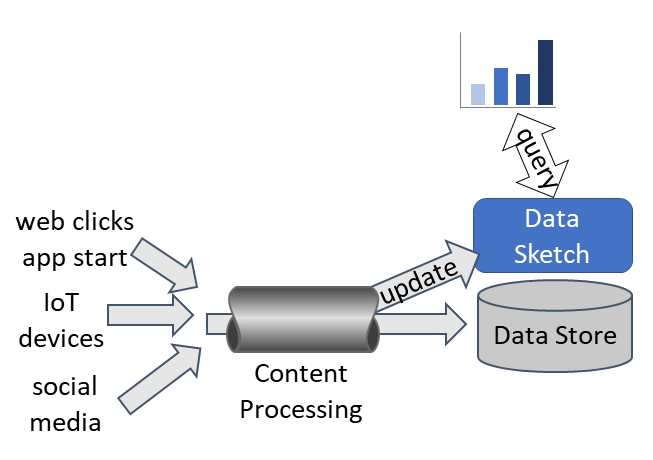
\includegraphics[height=1.6in]{graphics/fast-concurrent/pipeline-crop.png}
  \caption{Stream processing pipeline with data sketch.}
  \label{fc-fig:pipeline}
  \end{subfigure}
  \begin{subfigure}[b]{.55\linewidth}
    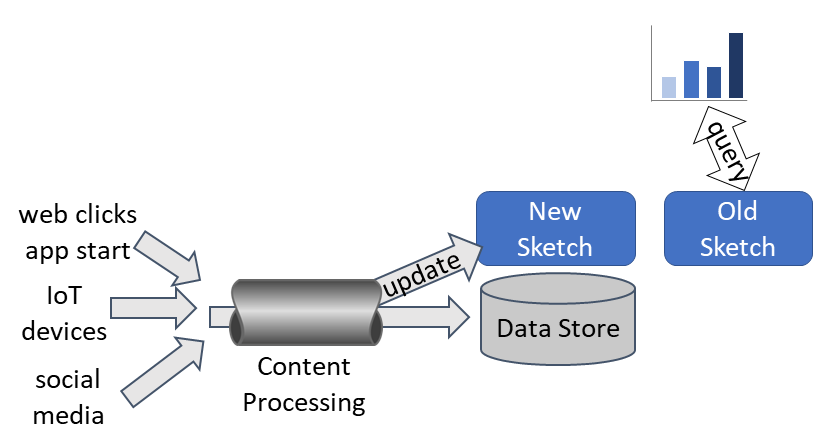
\includegraphics[height=1.6in]{graphics/fast-concurrent/epochs-crop.png}
  \caption{Using sketches in epochs.}
  \label{fc-fig:epochs}
  \end{subfigure}
\end{figure}

A sketch data structure is essentially a succinct (sublinear) summary of a stream that approximates a specific query, for instance, unique element count, quantile values, or frequent items. 
The approximation is typically very accurate -- the error drops fast with the stream size~\cite{Cormode:2017}. 

% Sketches today are sequential
Practical sketch implementations have recently emerged in toolkits~\cite{DataSketches}
and data analytics platforms (e.g., PowerDrill~\cite{heule2013hyperloglog}, Druid~\cite{druid}, 
Hillview~\cite{hillview}, and Presto~\cite{PrestoHLL}). 
However, these implementations are not thread-safe, allowing neither
parallel data ingestion nor concurrent queries and updates; concurrent use is prone to exceptions and 
gross estimation errors. Applications using these libraries are therefore required to explicitly protect all sketch API calls by locks~\cite{lee-groups-post, lee-issue}.
As a consequence of this limitation, typical deployments create sketches in epochs, where queries are referred to the sketch created in the previous epoch while new stream elements are directed to a new sketch, as illustrated in Figure~\ref{fc-fig:epochs}. This practice leads to stale query results and thus
loses the real-time quality of the system.  

\paragraph{Our approach.}
We present a generic approach to parallelizing data sketches efficiently while bounding the error that such a parallel implementation might induce. Our goal is to enable simultaneous queries and updates to the same sketch from multiple threads. Our solution is carefully designed to do so without slowing down operations as a result of synchronization.
This is particularly challenging because sketch libraries are extremely fast, often processing tens of millions of updates per second. 

We capitalize on the well-known sketch \emph{mergeability} property~\cite{Cormode:2017}, which enables computing a sketch 
over a stream by merging sketches over sub-streams. Previous works have exploited this property for distributed 
stream processing (e.g.,~\cite{heule2013hyperloglog, cormode2011algorithms}), devising solutions with a sequential bottleneck at the merge phase and where queries cannot
be served before all updates complete. 
In contrast, our method is based on shared memory and constantly propagates results to a queryable sketch.
Our solution architecture is illustrated in Figure~\ref{fc-fig:arch}. Multiple worker thread buffer updates in local sketches and periodically merge them into a global sketch; queries access the latter. 

\begin{figure}[htb]
  \begin{center}
    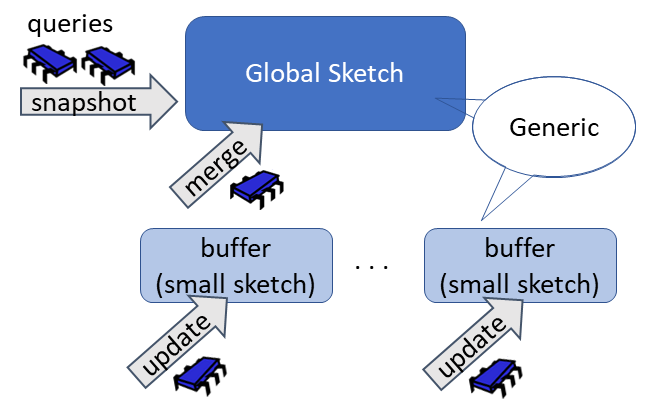
\includegraphics[width=0.5\textwidth]{graphics/fast-concurrent/arch-crop.png}
  \end{center}
  \caption{Concurrent sketches architecture.}
  \label{fc-fig:arch}
\end{figure}


We adaptively parallelize  stream processing:  
for small streams, we forgo parallel ingestion as it might introduce significant errors;  
but as the stream becomes large, we process it in parallel using small
thread-local sketches with continuous background propagation of local results to the common (queryable) sketch.

We instantiate our generic algorithm with a KMV $\Theta$ sketch~\cite{KMV},
which estimates the number of unique elements in a stream; a popular sketch
from the open-source Apache DataSketches library~\cite{DataSketches}.
We have contributed our implementation back to the Apache DataSketches 
library~\cite{ConcurrentThetaImp}. 
Yet we emphasize that our design is generic and applicable to additional sketches. 
We briefly discuss the applicability of our algorithm to additional popular sketches, such as Quantiles, CountMin, and HyperLogLog, 
where we discuss the generic algorithm (cf.~Section~\ref{fc-sec:genericAlg}).

Figure~\ref{fc-fig:performance} compares
the ingestion throughput of our concurrent $\Theta$ sketch to that of a lock-protected sequential sketch,
on multi-core hardware. As expected, the trivial solution does not scale whereas our algorithm scales linearly. 


\begin{figure}[htb]
  \begin{center}
    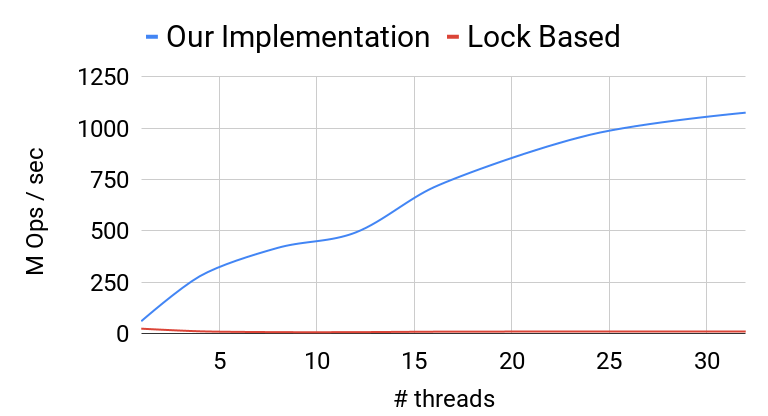
\includegraphics[width=0.6\textwidth]{graphics/fast-concurrent/concurrentThetaGraph.png}
  \end{center}
  \caption{Scalability of DataSketches' $\Theta$ sketch 
   protected by a lock vs.\ our concurrent implementation.}
  \label{fc-fig:performance}
\end{figure}

\paragraph{Error analysis.}
Concurrency might induce an error, and one of the main challenges we address is analyzing this error.
To begin with, our concurrent sketch is a concurrent data structure, and 
we need to specify its  semantics. We do so using a flavor of 
%\emph{relaxed consistency} due to Henzinger et al.~\cite{Henzinger}    
\emph{relaxed consistency} similar to~\cite{Henzinger, alistarh2018distributionally, talmage2014improving}    %specifically, a restricted form of their   \emph{out-of-order} relaxation 
that allows operations to ``overtake'' some other operations.  
Thus, a query may return a result that reflects all but a bounded number of the updates
that precede it. 
While relaxed semantics were previously used for data structures such as stacks~\cite{Henzinger}
and priority queues~\cite{alistarh, rihani2014multiqueues}, we believe that they are a natural fit for data sketches. 
This is because sketches are typically used to summarize streams that  arise from multiple real-world sources  
and are collected over a network with variable delays, and so even if the sketch ensures strict semantics, 
queries might miss some real-world events that occur before them. Additionally, sketches are inherently approximate.
Relaxing their semantics therefore ``makes sense'', as long as it does not excessively increase the expected error.
%Add that the error is addative and not multplicative
If a stream is much longer than the relaxation bound, then indeed the error induced by the relaxation is negligible. For instance, in a stream consisting of ten million events, missing a hundred (or even a thousand) of them will not make a big impact. 

Analytics platforms often use multiple sketches in order to capture different dimensions of the data. For instance, they may count the number of unique users from each region in a different sketch. 
Typically, a handful of popular sketches account for most events, and others are updated less frequently. Whereas the relaxation does not significantly affect the estimation in the popular sketches, since the error allowed by the relaxation is additive, in less popular sub-streams, it may have a large impact. 
This motivates our adaptive solution, which forgoes relaxing small streams altogether. 

% correctness roadmap: derandomise,  strong serialisability, Adversary model,

We show that under parallel ingestion, our algorithm satisfies relaxed consistency with a relaxation of up to $2Nb$, where $N$ is the number of worker threads and $b$ is the buffer size of each worker.  
In our example use case, $N$ is $12$ and $b$ ranges between $1$ and $5$. 

% But this raises a new difficulty: 
The proof involves some technical challenges. First, relaxed consistency is defined with regards to a deterministic specification, whereas sketches are randomized.
We therefore first de-randomize the sketch's behavior
by delegating the random coin flips to an oracle. We can then relax the resulting sequential specification.
Next, because our concurrent sketch is used within randomized algorithms, 
it is not enough to prove its linearizability. Rather, 
we prove that our generic concurrent algorithm instantiated with sequential sketch $S$
satisfies \emph{strong linearizability}~\cite{Wojciech} with regards to a relaxed sequential specification of the de-randomized $S$. We note, however, that supporting strong linearizability
did not incur additional costs nor did it impact the relaxation; we were able to prove that our original design was strongly linearizable. 

We then analyze the error for two types of relaxed sketches under random coin flips, with an adversarial scheduler that may delay operations in a way that maximizes the error. First, we consider the $\Theta$ sketch. For this sketch, its relative standard error has been analyzed, and we
show  that our concurrent implementation's error is coarsely bounded by twice
that of the corresponding sequential sketch. Second, we consider a family of \emph{probably approximately correct (PAC)}
sketches -- these are sketches that estimate some quantity with an error of at most $\epsilon$ with a probability of at least $1-\delta$. 
For an arbitrary PAC sketch estimating quantiles or counting unique elements, we show that the error induced by its relaxation approaches that of the original, non-relaxed sketch as the stream size tends to infinity.

\paragraph{Main contribution.} In summary, this paper tackles the problem of concurrent sketches,
offers a general efficient solution for it, and rigorously analyses this solution. While the
paper makes use of many known techniques, it combines them in a novel way.
The main technical challenges we address are (1) devising a high-performance generic algorithm 
that supports real-time queries concurrently with updates without inducing an excessive error; 
(2) proving the relaxed consistency of the algorithm; 
and (3) bounding the error induced by the relaxation in both short and long streams.

The paper proceeds as follows:
Section~\ref{fc-sec:model} lays out the model for our work and Section~\ref{fc-sec:background} provides background
on sequential sketches. In Section~\ref{fc-sec:concurrentSketches} we formulate a flavor of relaxed semantics
appropriate for data sketches. Section~\ref{fc-sec:genericAlg} presents our generic algorithm, and Section~\ref{fc-sec:proofs}
proves strong linearizability of our generic algorithm. Section~\ref{fc-sec:error-bounds} analyses
error bounds for example sketches. Section~\ref{fc-sec:eval} empirically studies the $\Theta$ sketch's performance
and error with different stream sizes. Finally, Section~\ref{fc-sec:discussion}
concludes.

\section{Model}
\label{fc-sec:model}

We consider a non-sequentially consistent shared memory model that enforces program order on all variables and allows explicit 
definition of \emph{atomic} variables as in Java~\cite{JavaMemoryModel} and C++~\cite{CppConcurrentMemoryModel}.
Practically speaking, reads and writes of atomic variables are guarded by memory fences, which guarantee
that all writes executed before a write {\sc w} to an atomic variable are visible to all
reads that follow (on any thread) a read {\sc r} of the same atomic variable s.t.\ {\sc r} occurs after {\sc w}. 


A thread takes \emph{steps} according to a deterministic \emph{algorithm} defined as a state machine, 
where a step can access a shared memory variable, do local computations, and possibly return some value.
%Every step is a 3-tuple  $\left\langle state, action, state' \right\rangle$ where \emph{action} is defined by the thread's state machine.
An \emph{execution} of an algorithm is an alternating sequence of steps and states, where  each step follows some thread's state machine.
Algorithms implement objects supporting \emph{operations}, such as query and update. 
An operation's execution consists of a series of steps, beginning with a special \emph{invoke} step and ending in a \emph{response}
step that may return a value. 
The \emph{history} of an execution $\sigma$, denoted ${\mathcal{H}}(\sigma)$, 
is its subsequence of operation invoke and response steps.
In a \emph{sequential history}, each invocation is immediately followed by its response.
The \emph{sequential specification (SeqSpec)} of an object is its set of allowed sequential histories.

%Correctness of concurrent algorithms is typically formulated using the notion of
%linearisability~\cite{herlihy1990linearizability}: 
A \emph{linearization} of a concurrent execution $\sigma$ is a history $H \in$\emph{SeqSpec}
such that (1) after adding responses to some pending invocations in $\sigma$ and removing others,
$H$ and $\sigma$ consist of the same invocations and responses (including parameters)
and (2) $H$ preserves the order between non-overlapping operations in $\sigma$.
Golab et al.~\cite{Wojciech} have shown that in order to ensure
correct behavior of randomized algorithms under concurrency,
one has to prove \emph{strong linearizability}:

\begin{definition}[Strong linearizability]
A function $f$ mapping executions to  histories is \emph{prefix preserving} if
for every  two executions $\sigma, \sigma'$ s.t.\ $\sigma$ is a prefix of $\sigma'$,  
$f(\sigma)$ is a prefix of $f(\sigma')$.

An algorithm $A$ is a strongly linearizable implementation of an 
object $o$ if there is a prefix preserving function $f$ that maps 
every execution $\sigma$ of $A$ to a linearization $H$ of $\sigma$.
\end{definition}

For example, executions of atomic variables are strongly linearizable.

\section{Background: sequential sketches}
\label{fc-sec:background}

A sketch $S$ summarizes a collection of elements $\Collection{a_1,a_2,\dots,a_n}$, processed
in some order given as a stream $A=a_1,a_2,\dots,a_n$.
The desired summary is agnostic to the processing order,
but the underlying data structures may differ due to the order. Its API is:

\begin{description}
\item[$S$.init()] initializes $S$ to summarize the empty stream;
\item[$S$.update($a$)] processes stream element $a$;
\item[$S$.query($arg$)] returns the function estimated by the sketch over the stream processed thus far, e.g., the number of unique elements; 
 takes an optional argument, e.g., the requested quantile.
 \item[$S$.merge($S'$)] merges sketches $S$ and $S'$ into $S$; i.e., if $S$ initially summarized stream $A$ and $S'$ 
 summarized $A'$, then after this call, $S$ summarizes the concatenation of the two, $A||A'$.
\end{description}

\paragraph{Example: $\Theta$ sketch.}

\begin{algorithm}[htb]
    \small
    %\begin{multicols}{2}
    \begin{algorithmic}[1]
        %\begin{varwidth}[t]{0.9\linewidth} 
        \Vars
        \State   sampleSet, init $k$ $1$'s \Comment samples
        \State  $\Theta$, init $1$			\Comment threshold
        \State {\tt atomic} est, init $0$ \Comment estimate
        \State $h$, init random uniform hash function 
        \EndFor
        
        \Procedure{query}{arg}
        \State \Return $est$ \label{fc-l:query}
        \EndProcedure
        
        \Procedure{update}{arg}
        \If{$h$(arg) $\geq \Theta$} \Return
        \EndIf
        \State add $h$(arg) to \emph{sampleSet}
        \State keep $k$ smallest samples in \emph{sampleSet}
        \State $\Theta \leftarrow max(sampleSet)$
        \State $\mathit{est}$ $\leftarrow $ $\left( |\text{sampleSet}|-1 \right)$ / $\Theta$
        \EndProcedure
        %\end{varwidth}\quad\quad\quad 
        %\columnbreak
        %\begin{varwidth}[t]{1\linewidth}

        \Procedure{merge}{S}
        \State sampleSet $\leftarrow$ merge sampleSet and $S$.sampleSet
        \State keep $k$ smallest values in sampleSet
        \State $\Theta \leftarrow max($sampleSet$)$
        \State $\mathit{est}$ $\leftarrow $ $\left( |\text{sampleSet}|-1 \right)$ / $\Theta$ \label{fc-l:update-est}
        \EndProcedure
        
    \end{algorithmic}
    %\end{multicols}
    \caption{$\Theta$ sketch.}
    \label{fc-alg:theta}
\end{algorithm}

Our running example is a $\Theta$ sketch based on the 
\emph{K Minimum Values (KMV)} algorithm~\cite{KMV} given in Algorithm~\ref{fc-alg:theta}. It maintains a \emph{sampleSet} and a parameter $\Theta$
that determines which elements are added to the sample set. 
It uses a random hash function $h$ whose outputs are uniformly distributed
in the range $[0,1]$, and $\Theta$ is always in the same range.  
An incoming stream element is first hashed, and then the hash is compared to $\Theta$. 
In case it is smaller, the value is added to \emph{sampleSet}.  Otherwise, it is ignored. 

Because the hash outputs are uniformly distributed, the expected proportion of values
smaller than $\Theta$ is $\Theta$. 
Therefore, we can estimate the number of unique elements in the stream by
dividing the number of (unique) stored samples by $\Theta$ (assuming that the random hash function is
drawn independently of the stream values).

KMV $\Theta$ sketches keep constant-size sample sets:
they take a parameter $k$ and keep the $k$ smallest hashes seen so far. 
$\Theta$ is $1$ during the first $k$ updates, and 
subsequently it is the hash of the largest sample in the set.
Once the sample set is full,
every update that inserts  a new element also removes the largest
one and updates $\Theta$. This is implemented efficiently using a min-heap.
The merge method adds a batch of samples to \emph{sampleSet}.

\paragraph{Accuracy.}

% Sequential specification
Today, sketches are used sequentially,
so that the entire stream is processed 
and then $S$.query(arg) returns an estimate of the desired function 
on the entire stream. Accuracy is defined in one of two ways.
One approach analyses the \emph{Relative Standard Error (RSE)} of the estimate, 
which is the standard error normalized by the quantity being estimated.
For example, a KMV $\Theta$ sketch with $k$ samples has an RSE of less than $1/\sqrt{k-2}$~\cite{KMV}.

 A PAC sketch provides a result that estimates the correct result
within some error bound $\epsilon$ with a failure probability bounded by some parameter $\delta$.  
For example, a Quantiles sketch approximates the $\phi$th quantile of a stream with $n$ elements 
by returning an element whose rank is in $\left[(\phi-\epsilon)n , (\phi+\epsilon)n \right]$ with 
probability at least $1-\delta$~\cite{agarwal2013mergeable}.

\section{Relaxed consistency for concurrent sketches}
\label{fc-sec:concurrentSketches}

Previous work by Alistarh et al.~\cite{alistarh2018distributionally} has presented a formalization for a randomized relaxation of an object.
The main idea is to have the parallel execution approximately simulate the object’s correct sequential behavior, with some provided error distribution.
In their framework, one considers the parallel algorithm and bounds the probability that it induces a large error
 relative to the deterministic sequential specification.
This approach is not suitable for our analysis, since the sequential object we parallelize (namely the sketch) is
itself randomized. Thus, there are two sources of error: (1) the approximation error in the sequential sketch and
(2) the additional error induced by the parallelization. For the former, we wish to leverage the
existing literature on analysis of sequential sketches. To bound the latter, we use a different
methodology: we first derandomize the sequential sketch by delegating its coin flips to an oracle,
and then analyze the relaxation of the (now) deterministic sketch. Finally, we leverage the sequential sketch
analysis to arrive at a distribution for the returned value of a query.


We adopt a variant of Henzinger et al.'s~\cite{Henzinger} {\emph{out-of-order}} relaxation,  
which generalizes quasi-linearizabilty~\cite{afek2010quasi}.
Intuitively, this relaxation allows a query to ``miss'' a bounded number of updates that precede it.
Because a sketch is order agnostic, we further allow re-ordering of the updates ``seen'' by a query.

\begin{definition}[r-relaxed history]
  A sequential history $H$ is an \emph{r-relaxation} of a sequential history $H'$,
  if $H$ is comprised of all but at most $r$ of the invocations in $H'$ and their responses,
  and each invocation in $H$ is preceded by all but at most $r$ of the invocations that precede the 
  same invocation in $H'$. 
\end{definition}

A relaxed property for an object $o$ is an extension of its sequential specification to include also
relaxed histories and thus allow more behaviors. This requires $o$ to have a sequential specification, so
we convert sketches into deterministic objects by capturing their randomness in an external oracle; 
given the oracle's output, the sketches behave deterministically.
For the $\Theta$ sketch, the oracle's output is passed as a hidden variable to $init$, where the sketch
selects the hash function. In the Quantiles sketch, a coin flip is provided with every update.

For a derandomized sketch, we refer to the set of histories arising in its sequential
executions as \emph{SeqSketch}, and use SeqSketch as its sequential specification.
We can now define our relaxed semantics:
\begin{definition}[r-relaxation]
The \emph{r-relaxation} of SeqSketch is the set of histories that have r-relaxations in SeqSketch:
  
\[ SeqSketch^r \triangleq \{H'|\exists H\in \textrm{SeqSketch s.t. H is an r-relaxation of}\ H'\}.\]

\label{fc-def:r-relaxtion}
\end{definition}

Note that our formalism slightly differs from that of~\cite{Henzinger} in that we start with a serialization $H'$ of an object’s
execution that does not meet the sequential specification and then ``fix'' it by relaxing it to a history $H$ in the sequential
specification. In other words, we relax history $H'$ by allowing up to $r$ updates to ``overtake'' every query, so the
resulting relaxation $H$ is in SeqSketch.
\begin{figure}[ht]
%\begin{wrapfigure}{r}{0.4\textwidth}
    \begin{center}
      %\vspace{-0.3in}
      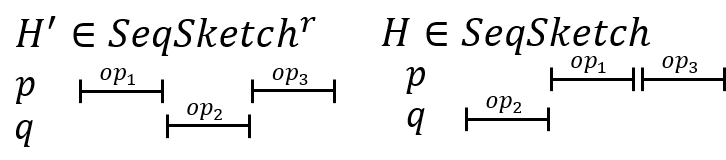
\includegraphics[width=0.5\textwidth]{graphics/fast-concurrent/relaxationExample}
      %\vspace{-0.3in}
    \end{center}
    \caption{$H$ is a 1-relaxation of $H'$.}
    \label{fc-fig:relaxationExample}
%\end{wrapfigure}
\end{figure}

An example is given in Figure~\ref{fc-fig:relaxationExample}, where $H$ is a 1-relaxation of history $H'$.
Both $H$ and $H'$ are sequential, as the operations don't overlap.
%In history $H$, $op_2$ has ``overtaken'' $op_1$ to appear first.

The impact of the $r$-relaxation on the sketch's error depends on the \emph{adversary}, which may select up to 
$r$ updates to hide from every query. There exist two adversary models:   
A \emph{weak adversary} decides which $r$ operations to omit from 
every query without observing the coin flips. 
A \emph{strong adversary} may select which updates to hide after learning 
the coin flips. Neither adversary sees the protocol's internal state, however both know the algorithm
and see the input. As the strong adversary knows the coin flips, it can then extrapolate the state; the
weak adversary, on the other hand, cannot.




\section{Generic concurrent sketch algorithm}
\label{fc-sec:genericAlg}

We now present our generic concurrent  algorithm. 
The algorithm uses, as a building block, an existing (non-parallel) sketch. 
To this end, we extend the standard sketch interface in Section~\ref{fc-sec:composable-sketches}, 
making it usable within our generic framework. That is, any sketch exposing this extended API can be used within our framework.
Our algorithm is adaptive -- it serializes ingestion in small streams and parallelizes it in large ones.
For clarity of presentation, we  present in Section~\ref{fc-sec:basic-generic-alg} the parallel phase of the algorithm,
which provides relaxed semantics appropriate for large streams.  
%in the full paper~\cite{rinberg2019fast}
%in Section~\ref{sec:proofs} we prove that it is strongly linearisable with respect to an $r$-relaxation of the sequential sketch with which it is instantiated.
Section~\ref{fc-ssec:small-streams} then discusses the adaptation for small streams.


\subsection{Composable sketches}
\label{fc-sec:composable-sketches}

In order to be able to build upon an existing sketch \emph{S},
we first extend it to support a limited form of concurrency.
Sketches that support this extension are called \emph{composable}.

A composable sketch has to allow concurrency between merges and queries.
To this end, we add a \emph{snapshot} API that can run concurrently with merge and
obtains a queryable copy of the sketch. The sequential specification of this operation is as follows:
\begin{description}
    \item[$S$.snapshot()] returns a copy $S'$ of $S$ such that immediately after $S'$ is returned,
     $S$.query($arg$) = $S'$.query($arg$) for every possible $arg$.
\end{description}

A composable sketch needs to allow concurrency only between snapshots
and other snapshot and merge operations. In general, we require that such concurrent
executions be strongly linearizable. Our $\Theta$ sketch, shown below,
simply accesses an atomic variable that holds the query result. In other sketches, for instance, 
CountMin~\cite{CountMin}, HyperLogLog~\cite{Flajolet07hyperloglog,heule2013hyperloglog,druid,PrestoHLL}, and Quantiles~\cite{KLL:2016}, atomic
snapshots can be achieved in a straightforward manner via a double collect of the relevant state, e.g., array of counters.
In specific sketches, this may be optimized in different ways. 

In recent work~\cite{rinberg_et_al:LIPIcs:2020:13080}, we have shown that for PAC objects, a linearizable snapshot is often not necessary for preserving the sketch's error bounds. We defined a relaxation of linearizability, called \emph{Intermediate Value Linearizability (IVL)}. We proved that for any sequential PAC object  -- that is, one guaranteeing an error of at most $\epsilon$ with a probability of at least $1-\delta$ for some parameters $\epsilon$ and $\delta$ -- any concurrent implementation of this object that satisfies IVL guarantees the same $\epsilon, \delta$ error bounds as the sequential object. In many cases, this allows replacing the linearizable snapshot with a single collect of the data structure, which is an array of counters in sketches like CountMin and HyperLogLog. In such cases, the implementation of the snapshot function is identical to the sequential sketch's query operation, and no synchronization is required. 

\paragraph{Pre-filtering.} When multiple sketches are used in a multi-threaded algorithm,
we can optimize them by sharing ``hints'' about the processed data.
This is useful when the stream sketching function depends on the processed stream prefix.
For example, we explain below how $\Theta$ sketches sharing a common value of $\Theta$ can sample fewer updates.
Another example is reservoir sampling~\cite{vitter1985random}. To support this optimization,
we add the following two APIs:
\begin{description}
    \item[$S$.calcHint()] returns a value $h \neq 0$ to be used as a hint.
    \item[$S$.shouldAdd($h$, $a$)] given a hint $h$ and a stream element $a$, returns a Boolean indicating whether $a$
		should be added to the sketch, or may be filtered out as it does not affect the sketch's state.
\end{description}    
%    Note that $S$.shouldAdd is a static function that does not depend on the current state of $S$.
    Formally, the semantics of these APIs are defined using the notion of summary.
		(1) Consider a sketch $S$ initialized in some state $s_0$. We say that $s_0$ (or the sketch at time $0$) \emph{summarizes} the empty history,
    and similarly, the empty stream; we refer to the sketch as \emph{empty}.
		(2) Let $s'$ be the sketch's state after we sequentially ingest a stream $a_1, \dots ,a_n$, namely after 		
		a sequential execution with the history 
		\[H= S.update(a_1), S.resp, \dots S.update(a_n), S.resp.\] 
		We say that $s'$ \emph{summarizes} history $H$, and,
    similarly, summarizes the stream $a_1, \dots ,a_n$.
    
		Given a sketch state $s'$ that summarizes a stream $A$, if shouldAdd($S.calcHint()$, $a$) returns false then
    for every streams $B_1,B_2$ and sketch state $s'$ that summarizes $A||B_1||a||B_2$,
    $s'$ also summarizes $A||B_1||B_2$. Note that a state summarizes two different streams if and only if that state is reached
		after ingesting each of them to an empty sketch.

These APIs do not need to support concurrency, and may be trivially implemented by always returning $true$.
Thus, they do not impose additional constraints on the set of sketches usable with our generic algorithm.


\paragraph{Example: composable $\Theta$ sketch.}
 
Algorithm~\ref{fc-alg:composable-theta} presents the three additional APIs for the $\Theta$ sketch.
The composable sketch is used concurrently by a single updater thread and multiple query threads. 
The \emph{est} variable is atomic, and is shared among all threads; the remaining state variables are local to the updating thread.

The snapshot method copies $\mathit{est}$. Note that the
result of a merge is only visible after writing to est, because it is the only variable accessed by
the query. As \emph{est} is an atomic variable, the requirement on snapshot and merge is
met. To minimize the number of updates, calcHint returns $\Theta$
and shouldAdd checks if $h(a) < \Theta$, which is safe because the value of
$\Theta$ in sketch $S$ is monotonically decreasing. Therefore, if $h(a) \geq \Theta$
then $h(a)$ will never enter the \emph{sampleSet}.

\begin{algorithm}[htb]
    \small
    %\begin{multicols}{2}
    \begin{algorithmic}[1]
       
        \Procedure{snapshot}{}
            \State $localCopy \leftarrow empty sketch$
            \State $localCopy.\mathit{est} \leftarrow \mathit{est}$
            \State \Return $localCopy$
        \EndProcedure
    
        \Procedure{calcHint}{}
            \State \Return $\Theta$
        \EndProcedure
    
        \Procedure{shouldAdd}{H, arg}
            \State \Return $h$(arg) $< H$
        \EndProcedure
    %\end{varwidth}

    \end{algorithmic}
    %\end{multicols}
    \caption{Additional methods for composable $\Theta$ sketch.}
    \label{fc-alg:composable-theta}
\end{algorithm}

\subsection{Generic algorithm}
\label{fc-sec:basic-generic-alg}

We now present a generic concurrent sketch algorithm that can be instantiated with any composobale sketch adhering to the API defined in the previous section. To simplify the presentation, we first discuss an unoptimized version of
our generic concurrent algorithm, (left column in of Algorithm~\ref{fc-alg:generic-concurrent}),  called 
\emph{ParSketch}, and later an optimized version of the same algorithm (right column of Algorithm~\ref{fc-alg:generic-concurrent}).

The algorithm is instantiated by a composable sketch and sequential sketches.
It uses multiple threads to process incoming stream elements 
and services queries at any time during the sketch's construction.
Specifically, it uses $N$ worker threads, $t_1,\dots,t_N$, each of which samples
stream elements into a local sketch $localS_i$, and a propagator thread $t_0$ that merges local sketches
into a shared composable sketch $globalS$. Although the local sketch resides in
shared memory, it is updated exclusively by its owner update thread $t_i$ and 
read exclusively by $t_0$. Moreover, updates and reads do not happen in
parallel, and so cache invalidations are minimized. The global sketch is updated only by $t_0$
and read by query threads. We allow an unbounded number of query threads. 

After $b$ updates are added to $localS_i$, $t_i$ signals to the propagator to merge
it with the shared sketch. It synchronizes with $t_0$ using a 
single \emph{atomic} variable $prop_i$, which $t_i$ sets to 0.  
Because $prop_i$ is atomic, the memory model
guarantees that all preceding updates to $t_i$'s local sketch are visible to
the background thread once $prop_i$'s update is.
This signalling is relatively expensive (involving a memory fence),  
but we do it only once per $b$ items retained in the local sketch.

After signalling to $t_0$, $t_i$ waits
until $prop_i \neq 0$  (line~\ref{fc-l:wait}); 
this indicates that the propagation has completed, and $t_i$ can 
reuse its local sketch. Thread $t_0$ piggybacks the hint \emph{H} it
obtains from the global sketch on $prop_i$,
and so there is no need for further synchronization in order to pass the hint.

Before updating the local sketch, $t_i$ invokes shouldAdd to check
whether it needs to process \emph{a} or not. For example, the $\Theta$ sketch discards updates whose hashes are
greater than the current value of $\Theta$. The global thread passes the global sketch's
value of $\Theta$ to the update threads, pruning updates that would end up being discarded
during propagation. This significantly
reduces the frequency of propagations and associated memory fences.

\begin{algorithm}[htb]
    \footnotesize
   \begin{multicols}{2}
    \begin{algorithmic}[1]
    \setcounter{ALG@line}{100}

     \Statex {\bf Basic algorithm } 
    \Vars
    \State composable sketch \emph{globalS}, init empty
    \State constant $b$ \Comment relaxation is $2Nb$
    \ForEach{update thread $t_i$} , $0 \leq i \leq N$
        \State sketch \emph{localS$_i$}, init empty
	\State
        \State int $counter_i$, init $0$
        \State int \emph{hint}$_i$, init $1$
        \State int {\tt atomic} $prop_i$, init $1$
    \EndFor
    \EndFor

    \Procedure{propagator}{}
    \While {true}
    \ForAll{thread $t_i$ s.t. $prop_i=0$}
        \State $globalS.merge(localS_i)$ \label{fc-l:merge}
        \State $localS_i  \leftarrow $empty sketch \label{fc-l:emptyAux}
		\State $prop_i \leftarrow globalS.calcHint()$ \label{fc-l:calcHint}
    \EndFor
    \EndWhile
    \EndProcedure

   

    \Procedure{query}{arg}
    \State $localCopy \leftarrow globalS.snapshot(localCopy)$
    \State \Return $localCopy.query(arg)$
    \EndProcedure
    
    \Procedure{update$_i$}{$a$}
    \If{$\neg$shouldAdd(\emph{hint}$_i$, $a$)} \Return \label{fc-l:shouldAdd}
    \EndIf
    \State $counter_i \leftarrow counter_i + 1$ \label{fc-l:countup}
    \State $localS_i.update(a)$ \label{fc-l:update}
    \If{$counter_i = b$} \label{fc-l:checkfull}
    \State {$prop_i \leftarrow 0$} \label{fc-l:signal}
    \State wait until $prop_i \neq 0$ \label{fc-l:wait}
     \State
    \State \emph{hint}$_i \leftarrow prop_i$ \label{fc-l:updateHint}
    \State $counter_i \leftarrow 0$ \label{fc-l:zeroCounter}
    \State
    \EndIf
    \EndProcedure

\columnbreak
    \setcounter{ALG@line}{200}
    \Statex {\bf Optimised algorithm } 
    \Vars
    \State composable sketch \emph{globalS}, init empty
    \State constant $b$ \Comment relaxation is $2Nb$
    \ForEach{update thread $t_i$} , $0 \leq i \leq N$
        \State sketch \emph{localS$_i$}[$2$], init empty
        \State int \emph{cur}$_i$, init 0
        \State int $counter_i$, init $0$
        \State int \emph{hint}$_i$, init $1$
        \State int {\tt atomic} $prop_i$, init $1$
    \EndFor
    \EndFor

    \Procedure{propagator}{}
    \While {true}
    \ForAll{thread $t_i$ s.t. $prop_i=0$}
        \State $globalS.merge(localS_i$[1-$cur_i$]$)$ 
        \State $localS_i[1-cur_i] \leftarrow $empty sketch 
		\State $prop_i \leftarrow globalS.calcHint()$ 
    \EndFor
    \EndWhile
    \EndProcedure
   
    \Procedure{query}{arg}
    \State $localCopy \leftarrow globalS.snapshot(localCopy)$
    \State \Return $localCopy.query(arg)$
    \EndProcedure
    
    \Procedure{update$_i$}{$a$}
    \If{$\neg$shouldAdd(\emph{hint}$_i$, $a$)} \Return 
    \EndIf
    \State $counter_i \leftarrow counter_i + 1$ 
    \State $localS_i$[$cur_i$]$.update(a)$ \label{fc-opt:l:update}
    \If{$counter_i = b$} \label{fc-opt:l:checkfull}
    \State 
    \State wait until $prop_i \neq 0$  \label{fc-opt:l:wait}
    \State $cur_i \leftarrow 1 - cur_i$ \label{fc-opt:l:swap-local-aux}
    \State \emph{hint}$_i \leftarrow prop_i$ \label{fc-opt:l:updateHint}
    \State $counter_i \leftarrow 0$ \label{fc-opt:l:zeroCounter}


    \State $prop_i \leftarrow 0$ \label{fc-opt:l:signal}
    \EndIf
    \EndProcedure


    \end{algorithmic}
   \end{multicols}
    \caption{Generic concurrent algorithm.}
    \label{fc-alg:generic-concurrent}
\end{algorithm}



Query threads use the snapshot method, which can be safely run concurrently with merge,
hence there is no need to synchronize between the query threads and $t_0$. The freshness
of the query is governed by the $r$-relaxation.
%In the full paper~\cite{rinberg2019fast},
In Section~\ref{fc-subsec:Generic-algorithm-proof}
we prove Lemma~\ref{fc-lemma:genereic-strong} below, asserting that
the relaxation is $Nb$. This may seem straightforward as $Nb$ is the combined size of the
local sketches. Nevertheless, proving this is not trivial because the local sketches pre-filter
many additional updates, which, as noted above, is instrumental for performance. 

\begin{lemma}
    $ParSketch$ instantiated with $SeqSketch$ is strongly linearisable with regards to  \emph{SeqSketch}$^r$, where
		$r=2Nb$.
    \label{fc-lemma:genereic-strong}
\end{lemma}


A limitation of \emph{ParSketch} is that update threads are idle while waiting for the propagator to execute the merge. This
may be inefficient, especially if a single propagator iterates through many local sketches.
In the right column of Algorithm~\ref{fc-alg:generic-concurrent}, we  present
the optimized \emph{OptParSketch} algorithm, which improves thread utilization via
double buffering.

In \emph{OptParSketch}, $localS_i$ is an array of two sketches. When $t_i$ is ready to propogate $localS_i[cur_i]$, it
flips the $cur_i$ bit denoting which sketch it is currently working on (line~\ref{fc-opt:l:swap-local-aux}), 
and immediately sets $prop_i$ to 0 (line~\ref{fc-opt:l:signal}) in order to allow the propagator to
take the information from the other one. It then starts digesting updates in a fresh sketch.

Of course, the optimization is only useful as long as the propagator thread is fast enough to empty the 
inactive buffers before the active ones fill up. The number of threads where this will saturate is highly sketch-dependant. 
In the example of the $\Theta$ sketch, thanks to pre-filtering, the working threads filter out many updates without filling their buffers, so
merges are required infrequently, and we can scale to a large number of threads with a single propagator regardless of the buffer size. In sketches without pre-filtering, the scalability typically depends on the buffer size.

In Section~\ref{fc-subsec:Optimised-algorithm-proof}
we prove the correctness of the optimized
algorithm by simulating $N$ threads of \emph{OptParSketch}
using $2N$ threads running \emph{ParSketch}. We do this by showing
a \emph{simulation relation}~\cite{lynch1996distributed}. We use forward simulation (with
no prophecy variables), ensuring strong linearizability. We conclude the following theorem:
\begin{restatable}{rthm}{optgenereicstrong}
    \emph{OptParSketch} instantiated with $SeqSketch$ is strongly linearizable with regards to \emph{SeqSketch}$^r$, where
		$r=2Nb$.
    \label{fc-lemma:opt-genereic-strong}
\end{restatable}


\subsection{Adapting to small streams}
\label{fc-ssec:small-streams}

By Theorem~\ref{fc-lemma:opt-genereic-strong}, a query can miss up to $r$ updates. For small
streams, the error induced by this can be very large.
For example, the sequential $\Theta$ sketch answers queries with perfect accuracy in streams with
up to $k$ unique elements, but if $k<r$, the relaxation can miss \emph{all} updates.
In other words, while the additive error is guaranteed to be bounded by $r$, the relative 
error can be infinite.  

To rectify this, we implement \emph{eager propagation} for small streams, 
whereby update threads propagate updates immediately to the shared sketch 
instead of buffering them. 
% and the shared sketch is accessed sequentially (protected by a lock or CAS).  
Note that during the eager phase, updates are processed sequentially. 
Support for eager propagation can be added to Algorithm~\ref{fc-alg:generic-concurrent} 
by initializing $b$ to $1$ and having the propagator thread raise it to the
desired buffer size once the stream exceeds some pre-defined length. 
The correctness of the adaptation is straightforward, since the buffer size is only used locally and only impacts the relaxation.
The error analysis of the next section can be used to determine the adaptation point.


\section{Proofs}
\label{fc-sec:proofs}

In Section~\ref{fc-sec:analysis:definitions} we introduce some formalisms.
In Section~\ref{fc-subsec:Generic-algorithm-proof} we prove that
the unoptimized algorithm is strongly linearizable with respect to
the relaxed specification $SeqSketch^r$ with $r=Nb$. Finally,
in Section~\ref{fc-subsec:Optimised-algorithm-proof} we show that
the the optimized algorithm is strongly linearizable with respect to
the relaxed specification $SeqSketch^r$ with $r=2Nb$.

\subsection{Definitions}
\label{fc-sec:analysis:definitions}
Note that the only methods invoked by $ParSketch$ on $globalS$ are snapshot and merge, and since merge is
only invoked by $t_0$, the only concurrency is between a snapshot and another operation (snapshot or merge).
Recall that we required such executions of a composable sketch to be strongly linearizable. By slight abuse
of terminology, we refer to these operations as atomic steps, for example, we refer to the linearization
point of $globalS$.merge simply as ``$globalS$.merge step''.

Likewise, as $localS_i$ is only accessed sequentially by a
single thread, either $t_i$ or $t_0$ (using $prop_i$ to synchronize),
we refer to the method calls shouldAdd and update as atomic steps.

Because we prove only safety properties, we restrict out attention to finite executions.
For analysis purposes we use auxiliary counters:
\begin{itemize}
    \item An array $sig\_ctr[N]$, that counts the number of times each thread $t_i$ signals to the propagator (line~\ref{fc-l:signal}).
    \item An array $merge\_ctr[N]$ counting the number of times $t_0$ executes a merge with thread $t_i$'s local sketch (line~\ref{fc-l:merge}).
\end{itemize}

Recall that in Section~\ref{fc-sec:background}, we said that a sketch's state \emph{summarizes} a
stream or a sequential history if it is the state of a sketch that has processed
the stream or history. We now overload the term ``summarizes'' to apply also to threads.
\begin{definition}[Thread summary]
    Consider a time $t$ in an execution $\sigma$ of Algorithm~\ref{fc-alg:generic-concurrent}. If at time $t$ either $prop_i \neq 0$
    or $sig\_ctr[i]>merge\_ctr[i]$, then we say that update thread $t_i$ \emph{summarizes} the history
    summarized by $localS_i$ at time $t$. Otherwise, thread $t_i$ summarizes the empty history at time $t$.
    The propagator thread $t_0$ summarizes the same history as $globalS$ at any time during an execution $\sigma$.
\label{fc-def:thread-summary}
\end{definition}
Note that if the first condition ($prop_i \neq 0$ or $sig\_ctr[i]>merge\_ctr[i]$) is not satisfied,
this means that the propagator thread might be in the process of clearing $localS_i$ in line~\ref{fc-l:emptyAux}.


As we want to analyze each thread's steps in an execution, we first define the projection from
execution $\sigma$ onto a thread $t_i$.
\begin{definition}[Projection]
    Given a finite execution $\sigma$ and a thread $t_i$, $\sigma\Bigr|_{t_i}$ is the subsequence of
    $\sigma$ consisting of steps taken by $t_i$.
\end{definition}

We want to prove that each thread's summary corresponds to the sequence of updates
processed by that thread since the last propagation, taking
into account only those that alter local state variables. These are updates for which \emph{shouldAdd} returns
true.
\begin{definition}[Unpropogated updates]
    Given a finite execution $\sigma$, we denote by suff$_i(\sigma)$ the suffix of $\sigma \Bigr|_{t_i}$ starting 
    at the last $globalS$.merge($localS_i$) event, or the beginning of $\sigma$ if no such event exists. 
    The unpropogated suffix up\_suff$_i(\sigma)$ of update thread $i$ is 
    the subsequence of $\mathcal{H} ($suff$_i(\sigma))$ consisting of $update(a)$ executions in suff$_i(\sigma)$ for which
    shouldAdd$(hint_i, arg)$ returns true in line \ref{fc-l:shouldAdd}.
    \label{fc-def:unpropogated-suffix}
\end{definition}

We define the relation between a sequential history $H$ and a stream $A$.
\begin{definition}
    Given a finite sequential history $H$, ${\mathcal{S}}(H)$ is the stream $a_1,\dots,a_n$ such that $a_k$
    is the argument of the $k$th update in $H$.
\end{definition}

Finally, we define the notion of \emph{happens before} in a sequential history $H$.
\begin{definition}
    Given a finite sequential history $H$ and two method invocations $M_1,M_2$ in $H$, we denote $M_1 \prec_H M_2$
    if $M_1$ precedes $M_2$ in $H$.
\end{definition}

\subsection{Unoptimized algorithm proof} 
\label{fc-subsec:Generic-algorithm-proof}

Our strong linearizability proof uses two mappings, $f$ and $l$, from 
executions to sequential histories defined as follows.
For an execution $\sigma$ of $ParSketch$, we define a mapping $f$ 
by ordering operations according to \emph{visibility points} defined as follows: 
\begin{itemize}
\item
For a query, the visibility point is the snapshot operation it executes.
\item 
For an update$_i$($a$) where shouldAdd($prop_i$, $a$) returns false at time $t$, its visibility point is $t$.
\item
Otherwise, for an update$_i$($a$), let $t$ be the first time after its invocation in $\sigma$
when thread $i$ changes $prop_i$ to 0 (line~\ref{fc-l:signal}).
Its visibility point is the (linearization point of the) first merge that occurs with $localS_i$ after time t.
If there is no such time, then update$_i$($a$) does not have a visibility point, i.e., is not included in $f(\sigma)$
\end{itemize}
Note that in the latter case,
the visibility point may occur after the update returns, and so $f$ does not 
necessarily preserve real-time order. 
 
We also define a mapping $l$ by ordering operations according to
\emph{linearization points} defined as follows:
\begin{itemize}
    \item
    An updates' linearization point is its invocation
    \item
    A query's linearization point is its visibility point.
\end{itemize}
By definition, $l(\sigma)$ is prefix-preserving.

We show that for every execution $\sigma$ of $ParSketch$,
(1) $f(\sigma) \in SeqSketch$, and 
(2) $f(\sigma)$ is an $r$-relaxation of $l(\sigma)$ for $r=N b$.  
Together, this implies that $l(\sigma) \in SeqSketch^r$, as needed.

We first show that $Prop_i \neq 0$ if $t_i$'s program counter is not on lines \ref{fc-l:signal} or \ref{fc-l:wait}.
\begin{invariant}
    At any time during a finite execution $\sigma$ of $ParSketch$ for every $i=1,\dots,N$, if $t_i$'s program
    counter isn't on lines \ref{fc-l:signal} or \ref{fc-l:wait}, then $prop_i \neq 0$.
    \label{fc-inv:prop-neq-0}
\end{invariant}
\begin{proof}
    The proof is derived immediately from the algorithm: $prop_i$ is initialized to 1 and gets
    the value of 0 on line \ref{fc-l:signal}, and then waits on line \ref{fc-l:wait} until $prop_i \neq 0$.
    After continuing passed line \ref{fc-l:wait}, $prop_i \neq 0$ again.
\end{proof}

We also observe the following:
\begin{observation}
    Given a finite execution $\sigma$ of $ParSketch$, for every $i=1,\dots,N$, every execution
    of $globalS.merge(localS_i)$ in $\sigma$ (line~\ref{fc-l:merge}) is preceded by an execution of $prop_i \leftarrow 0$
    (line~\ref{fc-l:signal}).
\end{observation}

We observe the following relationship between $t_i$'s program counter and $sig\_ctr[i]$ and \linebreak
$merge\_ctr[i]$:
\begin{observation}
    At all times during a finite execution $\sigma$ of $ParSketch$, for every
    $i=1,\dots,N$, $merge\_ctr[i] \leq sig\_ctr[i] \leq merge\_ctr[i] + 1$.
    Moreover, if $t_i$'s program counter isn't on lines \ref{fc-l:signal} or \ref{fc-l:wait}, then $sig\_ctr[i]=merge\_ctr[i]$.
    \label{fc-obs:counter_relationship}
\end{observation}

We show that at every point in an execution, update thread $t_i$ summarizes up\_suff$_i(\sigma)$. 
In essence, this means that we have not ``forgotten" any updates.
\begin{invariant}
    At all times during a finite execution $\sigma$ of $ParSketch$, for every $i=1,\dots,N$, $t_i$ summarizes up\_suff$_i(\sigma)$.
    \label{fc-inv:update-thread-summary}
\end{invariant}
\begin{proof}
    The proof is by induction on the length of $\sigma$. The base is immediate.
    Next we consider a step in $\sigma$ that can alter the invariant. We assume the invariant is correct
    for $\sigma'$, and prove correctness for $\sigma=\sigma',step$. We consider only steps that
    can alter the invariant, meaning the step can 
    either lead to a change in up\_suff$_i(\sigma)$, or a change in the history summarized by $t_i$. This
    means we need to consider only 4 cases:
    \begin{itemize}

        \item A step $localS_i.update(arg)$ (line~\ref{fc-l:update}) by thread $t_i$.

        In this case, up\_suff$_i(\sigma)=$up\_suff$_i(\sigma'),update(arg)$.
        By the inductive hypothesis, before the step $localS_i$ summarizes up\_suff$_i(\sigma')$,
        and so after the update, $localS_i$ summarizes $\text{up\_suff}_i(\sigma'),$ \linebreak $update(arg)=\text{up\_suff}_i(\sigma)$.
        From Invariant~\ref{fc-inv:prop-neq-0} $prop_i \neq 0$, therefore, by Definition \ref{fc-def:thread-summary}, $t_i$ summarizes
        the same history as $localS_i$,
        i.e., up\_suff$_i(\sigma)$, preserving the invariant.

        \item A step $prop_i \leftarrow 0$ (line~\ref{fc-l:signal}) by thread $t_i$.
        
        By the inductive hypothesis, before the step, $t_i$ summarizes the 
        history up\_suff$_i(\sigma')$. Because before the step  $prop_i \ne 0$, $localS_i$ 
				summarizes the same history.
        As no update occurs, up\_suff$_i(\sigma')$=up\_suff$_i(\sigma)$. The step
        doesn't alter $localS_i$, so after the step, $localS_i$ still summarizes
        up\_suff$_i(\sigma)$. On this step the counter $sig\_ctr[i]$ is increased but $merge\_ctr[i]$
        is not, so $sig\_ctr[i]>merge\_ctr[i]$.
        Therefore, by Definition \ref{fc-def:thread-summary}, $t_i$ summarizes the same history as $localS_i$,
        namely up\_suff$_i(\sigma)$, preserving the invariant.

        \item A step $globalS.merge(localS_i)$ (line~\ref{fc-l:merge}) by thread $t_0$.
        
        By Definition~\ref{fc-def:unpropogated-suffix}, after this step up\_suff$_i(\sigma)$ is empty. As
        this step is a $merge$, $merge\_ctr[i]$ is increased by one, so $sig\_ctr[i]=merge\_ctr[i]$ by
        Observation~\ref{fc-obs:counter_relationship}.
        Therefore, by Definition \ref{fc-def:thread-summary}, $t_i$
        summarizes the empty history, preserving the invariant.

        \item A step $prop_i \leftarrow globalS.calcHint()$ (line~\ref{fc-l:calcHint}) by thread $t_0$
        
        Before executing the step, $t_0$ executed line~\ref{fc-l:emptyAux}. Thread $t_i$ is waiting
        for $prop_i \neq 0$ on line~\ref{fc-l:wait}, therefore has not updated $localS_i$.
        Therefore, by Definition~\ref{fc-def:thread-summary}, $localS_i$ summarizes the empty history.
        As a merge with thread $i$ was executed and no updates have been invoked, up\_suff$_i(\sigma)$
        is the empty history.
        The function $calcHint$ cannot return $0$, therefore after that step $prop_i \neq 0$.
        By Definition \ref{fc-def:thread-summary}, $t_i$ summarizes the same history as $localS_i$, i.e., the empty history.
        Therefore, $t_i$ summarizes up\_suff$_i(\sigma)$, preserving the invariant.
    \end{itemize}
\end{proof}

Next, we prove that $t_0$ summarizes $f(\sigma)$.
\begin{invariant}[History of propagator thread]
    Given a finite execution $\sigma$ of $ParSketch$, $t_0$ summarizes $f(\sigma)$.
    \label{fc-inv:G-partial-summary}
\end{invariant}
\begin{proof}
    The proof is by induction on the length of $\sigma$. The base is immediate.
    We assume the invariant is correct for $\sigma'$, and prove correctness for $\sigma=\sigma',step$.
    There are two steps that can alter the invariant.
    \begin{itemize}
        \item A step $globalS.merge(localS_i)$ (line~\ref{fc-l:merge}) by thread $t_0$.
        
        By the inductive hypothesis, before the step, $t_0$ summarizes $f(\sigma')$. And by
        Invariant~\ref{fc-inv:update-thread-summary}, before the update, $t_i$ summarizes
        up\_suff$_i(\sigma')$, and by Invariant~\ref{fc-inv:prop-neq-0} $localS_i$ summarizes the same history.
        Let $A={\mathcal{S}}(f(\sigma))$, and $B={\mathcal{S}}($up\_suff$_i(\sigma')$$)$.
        After the merge $globalS$ summarizes $A||B$. Therefore,
        $t_0$ summarizes $f(\sigma)$ preserving the invariant.

        \item A step shouldAdd($prop_i$, $a$) (line~\ref{fc-l:shouldAdd}) by thread $t_i$, returning false.     
        
        Let $H$ be that last hint returned to $t_i$, and let $\sigma''$ be the prefix of $\sigma$ up to this point.
        By the induction hypothesis, at that point $globalS$ summarized $f(\sigma'')$.
        Let $A=\mathcal{S}$$(f(\sigma''))$, and let $B=\mathcal{S}$$(f(\sigma'))$,
        and let $B_1$ be such that $B=A||B_1$. By the induction hypothesis,
        before the step, $globalS$ summarizes $B=A||B_1$.
        By the assumption of \emph{shouldAdd}, if shouldAdd($H$, $arg$) returns false, then if
        a sketch summarizes $B=A||B_1||B_2$, then it also summarizes $B=A||B_1||a||B_2$. Let
        $B_2=\emptyset$, then $globalS$ summarizes $B=A||B_1||B_2$, therefore also summarizes 
        $A||B_1||a||B_2=A||B_1||a$. Therefore, after the step, $globalS$ summarizes $f(\sigma)$
        preserving the invariant.
    \end{itemize}
\end{proof}

To finish the proof that $f(\sigma) \in SeqSketch$, we prove that a query invoked at the end of $\sigma$
returns a value equal to the value returned by a sequential sketch after processing $A={\mathcal{S}}(f(\sigma))$.
\begin{lemma}[Query Correctness]
    Given a finite execution $\sigma$ of $ParSketch$, let $Q$ be a query that returns
    in $\sigma$, and let $v$ be $Q$'s visibility point. Let $\sigma'$ be the prefix
    of $\sigma$ until point $v$, and let $A={\mathcal{S}}(f(\sigma'))$. $Q$ returns a value
    that is equal to the value returned by a sequential sketch after processing $A$.
    \label{fc-lemma:query-correctness}
\end{lemma}
\begin{proof}
    Let $\sigma$ be an execution of $ParSketch$, and let $Q$ be a query that returns in $\sigma$.
    Let $\sigma'$ and $A$ be as defined in the lemma. By Invariant \ref{fc-inv:G-partial-summary}, 
    $t_0$ summarizes $f(\sigma')$ at point $v$, therefore \emph{globalS} 
    summarizes $f(\sigma')$ at the same point, therefore \emph{globalS} summarizes 
    stream $A$ at point $v$. The visibility point for the query, at point $v$,
    is $globalS.$snapshot$()$. By the requirement from $S$.snapshot(), for all $arg$ 
    $globalS.query(arg)=localCopy.query(arg)$. Because $globalS$ summarizes
    stream $A$, $localCopy.query(arg)$ returns a value equal to the value
    returned by the sequential sketch $globalS$ after processing $A$.
\end{proof}

As we have proven that each query in $f(\sigma)$ returns a value that estimates all
the updates that happen before its invocation, we have proven the following:
\begin{lemma}
    Given a finite execution $\sigma$ of $ParSketch$, $f(\sigma) \in SeqSketch$.
    \label{fc-lemma:f-in-seqsketch}
\end{lemma}

To complete the proof, we prove that $f(\sigma)$ is an $r$-relaxation of $l(\sigma)$, for $r=Nb$.
We begin by proving orders between queries and other method calls.
\begin{lemma}
    Given a finite execution $\sigma$ of $ParSketch$, and given an operation $O$(query or update) in $l(\sigma)$,
    for every $Q$ in $l(\sigma)$ such that $Q \prec_{l(\sigma)} O$,
    then $Q \prec_{f(\sigma)} O$.
    \label{fc-lemma:QueryOrders}
\end{lemma}
\begin{proof}
    If $O$ is a query,
    then proof is immediate from the definitions of $l$ and $f$.
    If $O$ is an update, then, by the definition of $f$, an updates visibility point
    is at the earliest its linearization point.
    As $Q$'s visibility point and linearization point are equal, it follows
    that if  $Q \prec_{l(\sigma)} O$ then $Q \prec_{f(\sigma)} O$.
\end{proof}

We next prove an upper bound on the number of updates in up\_suff$_i(\sigma)$. We denote the
number of updates in history $H$ as $\abs{H}$.
\begin{lemma}
    Given a finite execution $\sigma$ of $ParSketch$, $\abs{\text{up\_suff}_i(\sigma)} \leq b$.
    \label{fc-lemma:update-thread-summary-bound}
\end{lemma}
\begin{proof}
    As $counter_i$ is incremented before an update which is included in $\text{up\_suff}_i(\sigma)$,
    it follows that $\abs{\text{up\_suff}_i(\sigma)} \leq counter_i$. When $counter_i = b$, $t_i$
    signals for a propagation (line~\ref{fc-l:signal}) and then waits until $prop_i \neq 0$ (line~\ref{fc-l:wait}).
    When $t_i$ finishes waiting, then it zeros the counter (line~\ref{fc-l:zeroCounter}) before ingesting
    more updates, therefore, $count_i \leq b$. Therefore, it follows that $\abs{\text{up\_suff}_i(\sigma)} \leq b$.
\end{proof}

As $f(\sigma)$ contains all updates with visibility points, we can now prove the following.
\begin{lemma}
    Given a finite execution $\sigma$ of $ParSketch$, $\abs{f(\sigma)} \geq \abs{l(\sigma)} - N$$b$.
    \label{fc-lemma:f-bound}
\end{lemma}
\begin{proof}
    From Lemma~\ref{fc-lemma:update-thread-summary-bound}, $\abs{\text{up\_suff}_i(\sigma)} \leq b$.
    The only updates without a visibility point are updates that are in up\_suff$_i(\sigma)$ for some $i$.
    Therefore $f(\sigma)$ contains all updates but any update in a history up\_suff$_i(\sigma)$ for some $i$.
    There are $N$ update threads, therefore $\abs{f(\sigma)} = \abs{l(\sigma)} - $$\sum_{i=1}^{N} \abs{\text{up\_suff}_i(\sigma)}$
    so $\abs{f(\sigma)} \geq \abs{l(\sigma)} - N $$b$.
\end{proof}

We will now prove that given an execution $\sigma$ of $ParSketch$, every invocation in $f(\sigma)$
is preceded by all but at most $Nb$ of the invocations in $l(\sigma)$.
\begin{lemma}
    Given a finite execution $\sigma$ of $ParSketch$, $f(\sigma)$ is an Nb-relaxation of $l(\sigma)$.
    \label{fc-lemma:f-relaxing-l}
\end{lemma}
\begin{proof}
    Let $\sigma$ be a finite execution of $ParSketch$, and consider an operation $O$ in $f(\sigma)$
    such that $O$ is also in $l(\sigma)$. Let $Ops = \Set{O'}{(O' \prec_{l(\sigma)} O) \wedge (O' \nprec_{f(\sigma)} O)}$.
    We show that $\abs{Ops} \leq Nb$.
    By Lemma~\ref{fc-lemma:QueryOrders}, for every query $Q$ in $l(\sigma)$ such that $Q \prec_{l(\sigma)} O$,
    then $Q \prec_{f(\sigma)} O$, meaning $Q \notin Ops$.
    Let $\sigma^{pre}$ be a prefix and $\sigma^{post}$ a suffix of $\sigma$ such that
    $l(\sigma)=l(\sigma^{pre}),O,l(\sigma^{post})$. From Lemma~\ref{fc-lemma:f-bound}, $\abs{f(\sigma^{pre})} \geq \abs{l(\sigma^{pre})} - Nb$.
    As $\abs{f(\sigma^{pre})}$ is the number of updates in $f(\sigma^{pre})$, and $\abs{l(\sigma^{pre})}$ is the number of updates
    in $l(\sigma^{pre})$, $f(\sigma^{pre})$ contains all but at most $Nb$ updates in $l(\sigma^{pre})$. As $l(\sigma^{pre})$
    contains all the updates that precede $O$. Meaning $Ops$ is all the updates in $l(\sigma^{pre})$ and not in
    $f(\sigma^{pre})$. Therefore, $\abs{Ops} = \abs{l(\sigma^{pre})} - \abs{f(\sigma^{pre})} \leq Nb$.
    Therefore, by Definition~\ref{fc-def:r-relaxtion}, $f(\sigma)$ is an $Nb$-relaxation of $l(\sigma)$.
\end{proof}

Putting together Lemma~\ref{fc-lemma:f-in-seqsketch} and Lemma~\ref{fc-lemma:f-relaxing-l}, we have shown that
given a finite execution $\sigma$ of $ParSketch$, $f(\sigma) \in SeqSketch$ and $f(\sigma)$ is an $Nb$-relaxation
of $l(\sigma)$. We have proven Lemma~\ref{fc-lemma:genereic-strong}.

\subsection{Optimized algorithm proof}
\label{fc-subsec:Optimised-algorithm-proof}
We denote the optimized version of Algorithm~\ref{fc-alg:generic-concurrent} as \emph{OptParSketch}. 
We prove the correctness of \emph{OptParSketch} by showing that it can simulate  \emph{ParSketch}. 
This proof technique is known as   a \emph{simulation relation}, which, as explained in~\cite{lynch1996distributed}, Chapter 2.5, 
is a correspondence relating the states of \emph{OptParSketch} and \emph{ParSketch} when the algorithms run on the same input stream. 
Establishing a simulation relation proves that $OptParSketch$ is strongly linearizable with regards to 
$SeqSketch^{2Nb}$~\cite{10.1016/j.tcs.2010.09.021,attiya2019putting}.

Consider an arbitrary worker thread $t_i$ for the optimized algorithm,
and simulate this thread using two worker threads $t_i^0,t_i^1$ of the basic algorithm.
%Algorithm~\ref{fc-alg:generic-concurrent}.
To simulate $N$ worker threads, we need $2N$ threads, and they are mapped the same way.

The idea behind the simulation is that there might be a delay between the time when the \emph{hint} is returned to the worker thread and the time when this hint is used for pre-processing, so we can simulate each thread by two threads. For example in Figure~\ref{fc-fig:optimisedSimulation},
each block $A_i$ is a stream such that $b$ updates pass the test of \emph{shouldAdd} (except maybe $A_n$).
The stream processed by $t_i$ is $A=A_1||A_2||\dots||A_n$ and we assume $n$ is even.
Each $A_i$ is evaluated against the \emph{hint} written above it. The thread $t_i^0$ simulates processing
$A_1||A_3||\dots ||A_{n-1}$, and thread $t_i^1$ simulates processing $A_2||A_4||\dots||A_n$.

\begin{figure}[H]
    \centering
    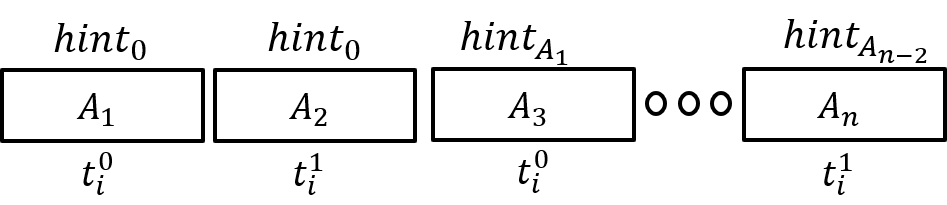
\includegraphics[width=4.2in]{graphics/fast-concurrent/optimisedSimulation.png}
    \caption{Simulation of processing $A=A_1||A_2||\dots||A_n$.}
    \label{fc-fig:optimisedSimulation}
\end{figure}

The simulation uses auxiliary variables oldHint$_i^0$, and oldHint$_i^1$, both initialized to 1.
These variables are updated with the flipping of $cur_i$ (line~\ref{fc-opt:l:swap-local-aux}), such that:
\begin{itemize}
    \item oldHint$_i^0$ is updated to be the current (pre-flip) value of $hint_i$
    \item oldHint$_i^1$ is updated to be the current (pre-flip) value of $oldHint_i^0$
\end{itemize}

%The simulation uses an auxiliary variable $oldHint_i^0$ initialised to 1. This variable is updated
%with the flipping of $cur_i$ (line~\ref{fc-opt:l:swap-local-aux}) with the current value of $hint_i$.

In addition, the simulation uses an auxiliary variable \emph{auxCount$_i$} initialized to 0. This variable is set to
$b$ before the first execution of line~\ref{fc-opt:l:swap-local-aux}, and is never changed after that. 

Finally, the simulation uses two auxiliary variables $PC_i^0$ and $PC_i^1$ to be
program counters for threads $t_i^0$ and $t_i^1$. They are initialized to \emph{Idle}.

We define a mapping $g$ from the state of $OptParSketch$ to the state of $ParSketch$ as follows:
\begin{itemize}
    \item \emph{globalS} in $OptParSketch$ is mapped to \emph{globalS} in $ParSketch$.
    \item localS$_i[j]$ is mapped to $t^j$.localS for $j=0,1$.
    \item counter$_i$ is mapped to $t^{cur_i}$.counter.
    \item auxCount is mapped to $t^{1-cur_i}$.counter.
    \item hint$_i$ is mapped to $t^{cur_i}$.hint and $t^{cur_i}$.prop if $t_i$ is not right before executing line 227,
    otherwise oldHint$_i^0$ is mapped to $t^{cur_i}$.hint and prop$_i$ is mapped to $t^{cur_i}$.prop.
    \item prop$_i$ is mapped to $t^{1-cur_i}$.prop if $t_i$ is not right before executing lines 227-229,
    otherwise oldHint$_i^1$ is mapped to $t^{1-cur_i}$.prop.
    \item oldHint$_i^1$ is mapped to $t^{1-cur_i}$.hint.
\end{itemize}

For example, Figure~\ref{fc-fig:optConcurrentMap} shows a mapping when $cur_i$ equals 0, before executing
line 227. Table~\ref{fc-table:opt-simulation} shows the steps taken by $t_i^0$ and $t_i^1$ when
$cur_i=0$ before line~223.

\begin{figure}[ht]
    \centering
    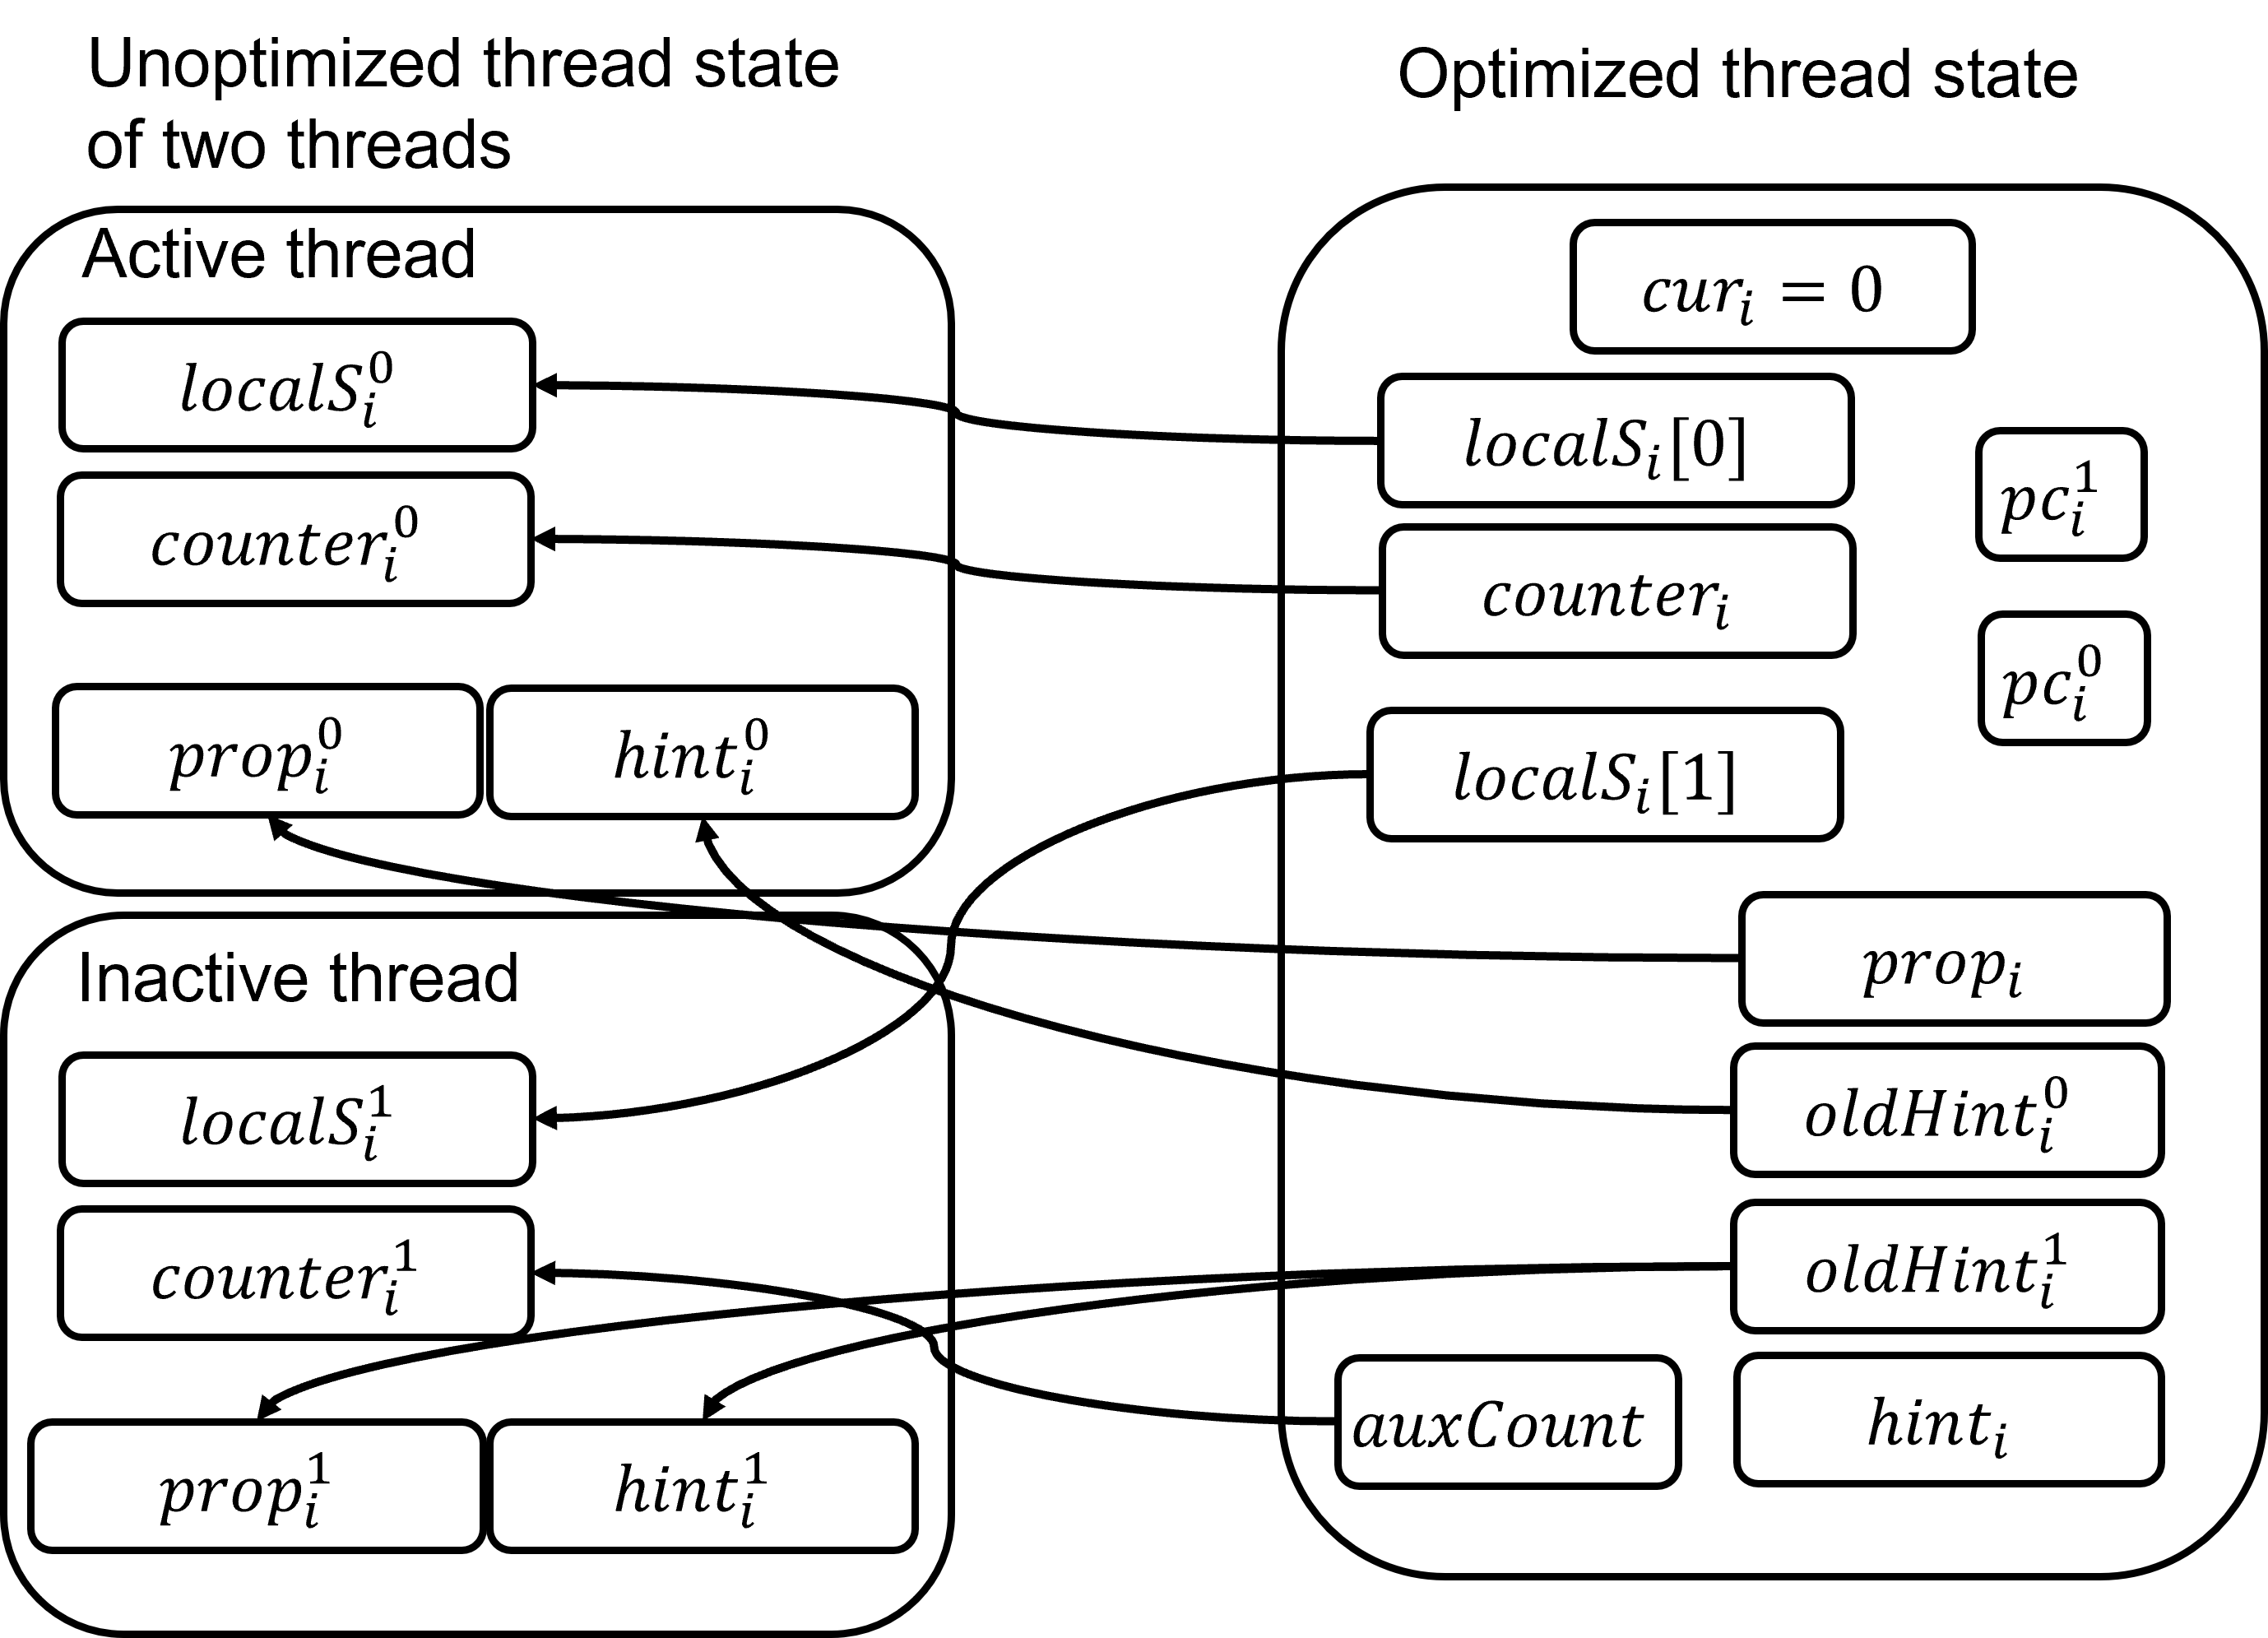
\includegraphics[width=5in]{graphics/fast-concurrent/optConcurrentMap.png}
    \caption{Reference mapping of $g$ when $cur_i$ equals 0 before executing line 227.}
    \label{fc-fig:optConcurrentMap}
\end{figure}

\begin{table}[H]
    \begin{tabular}{c|c|c}
        \emph{OptParSketch} line & \emph{ParSketch} line & Executing thread\\[5pt]
        \hline
        \ref{fc-opt:l:checkfull} & \ref{fc-l:checkfull} & $t_i^0$\\[5pt]
        \ref{fc-opt:l:wait} & \ref{fc-l:wait}& $t_i^1$\\[5pt]
        \ref{fc-opt:l:swap-local-aux} & - & - \\[5pt]
        \ref{fc-opt:l:updateHint} & \ref{fc-l:updateHint} & $t_i^1$\\[5pt]
        \ref{fc-opt:l:zeroCounter} & \ref{fc-l:zeroCounter} & $t_i^1$\\[5pt]
        \ref{fc-opt:l:signal} & \ref{fc-l:signal} & $t_i^0$ 
    \end{tabular}
    \caption{Example for steps taken by $t_i^0$ and $t_i^1$ for each step taken by $t_i$ when $cur_i=0$ before line~\ref{fc-opt:l:checkfull},
    meaning the ``round'' of $b$ updates was ingested by $t_i^0$. On line~\ref{fc-opt:l:swap-local-aux} neither thread takes a step.}
    \label{fc-table:opt-simulation}
\end{table}

We also define the steps taken in $ParSketch$ when $OptParSketch$ takes a step. If a \emph{query} is invoked,
then both algorithms take the same step. If an \emph{update} in invoked, the  \emph{update} is invoked in
$t_i^{cur_i}$ in $ParSketch$. If the counter gets up to $b$ (meaning we get to line~\ref{fc-opt:l:wait}), then
$t_i^{1-cur_i}$ executes line~\ref{fc-l:wait}. When $OptParSketch$ flips $cur_i$ (line~\ref{fc-opt:l:swap-local-aux}),
then neither of the threads $t_i^0$ or $t_i^1$ take a step. Afterwards, lines \ref{fc-opt:l:updateHint} and \ref{fc-opt:l:zeroCounter} execute the corresponding lines (\ref{fc-l:updateHint} and \ref{fc-l:zeroCounter}) 
on thread $t_i^{cur_i}$, and line \ref{fc-opt:l:signal} executes \ref{fc-l:signal} on thread $t_i^{1-cur_i}$.

\begin{lemma}
    $g$ is a simulation relation from $OptParSketch$ to $ParSketch$.
\end{lemma}
\begin{proof}
The proof is by induction on the steps in an execution, for some thread $i$. In the initial state, the mapping trivially holds.
In a given step, we refer to $t_i^{cur_i}$ as the \emph{active} thread and $t_i^{1-cur_i}$ as the \emph{inactive thread}. 
Query threads trivially map to themselves and do not alter the state. We next consider update and propagator threads. 
First, consider the steps of OptParSketch that execute the corresponding step on the active thread.
These are lines 219--223 and 227--228, which directly correspond to lines 119-123 and 127-128 of ParSketch in the
active thread ($t_i^{cur_i}$), and, except in lines 127 and 129, the effected state variables are mapped to the
same state variables in the active thread. So these steps trivially preserve $g$.
Line 124 in \emph{ParSketch} is executed on the inactive thread when \emph{OptParSketch} executes line 229. As after
this step the inactive thread's prop and prop$_i$ are both $0$, so $g$ is preserved. 
Line 125 is executed on the inactive thread, waiting on the same variable, and modifies no variables, so $g$ is preserved.

Line 226 flips $cur_i$ and neither thread takes a step in \emph{ParSketch}. Here, the mappings of $prop$, $hint$, and $counter$ change. 
On this step oldHint$_i^0$ and oldHint$_i^1$ are updated as defined, and as $t_i$ is right before
executing line 227, oldHint$_i^1$ is equal to the inactive thread's ($t_i^{1-cur_i}$) hint, and, as before the step the (now)
inactive thread's prop was equal to hint$_i$, then after this step it is equal to oldHint$_i^0$.
As before the step the (now) active thread's hint was equal to oldHint$_i^0$, after this step it is equal to oldHint$_i^1$. Finally,
as before the step the (now) active thread's prop was equal to prop$_i$, after this step it remains equal to prop$_i$, so this
step preserve $g$.

In line 227, hint$_i$ gets the value of prop$_i$, and the same happens on the active thread. As before this line the
active thread's prop was equal to prop$_i$, after this step the inactive thread's prop and hint are equal to hint$_i$,
preserving $g$.
As the active thread's counter is equal to $counter_i$, line 228 preserves $g$.
The now inactive thread has filled its local sketch, therefore its counter is $b$, which equals
auxCount.  
Finally, the propagator thread’s steps (lines 210-215) execute on the inactive
thread and it is easy to see that all variables accessed in these steps are mapped to the same variables in the inactive thread. 
\end{proof}

Note that the simulation relation uses no prophecy variables, i.e., does not ``look into the future''.
This establishes strong linearizability~\cite{attiya2019putting}, intuitively, because 
the mapping of all ParSketch’s steps -- including linearization points --  to steps in OptParSketch is prefix-preserving.
Since we use two update threads of ParSketch to simulate one thread in OptParSketch, we have proven the following theorem:

\optgenereicstrong*

\section{Deriving error bounds}
\label{fc-sec:error-bounds}

We now show how to translate the $r$-relaxation to a bound on the error of typical sketches.
We consider two types of error anlayzes of existing sketches. In Section~\ref{fc-ssec:theta-analysis}, we consider the 
relative standard error of the $\Theta$ sketch, which was used in the original analysis of the sketch.  
In Section~\ref{fc-ssec:quantiles-error-analysis} we consider PAC sketches, and show generic error bounds for all $r$-relaxed 
implementations of PAC sketches estimating the number of unique elements and quantiles.  

%We bound the error induced by the relaxation on two representative sketches.
%Section~\ref{fc-ssec:RSE-RMSE} formally defines the RSE and RSME metrics.
%Section~\ref{fc-ssec:theta-analysis} discusses the error introduced to the
%expected estimation and RSE of the KMV $\Theta$ sketch.
%Section~\ref{fc-ssec:quantiles-error-analysis} analyses the PAC Quantiles sketch.



\subsection{\texorpdfstring{$\Theta$}{Theta} error bounds}
\label{fc-ssec:theta-analysis}

We bound the error introduced by an $r$-relaxation of the $\Theta$ sketch over a stream with $n$ unique elements and a parameter (sketch size) of $k$. Given
Theorem~\ref{fc-lemma:opt-genereic-strong}, the optimized concurrent sketch's error is bounded
by the relaxation's error bound for $r=2Nb$. We consider strong and weak adversaries,
${\mathcal{A}}_s$ and ${\mathcal{A}}_w$, resp. For the strong adversary we are able to show only numerical
results, whereas for the weak one we show closed-form bounds. The results are summarized in Table~\ref{fc-table:Theta-Error-Summary}.
Our analysis relies on known results from order statistics~\cite{david2004order}.
It focuses on long streams, and assumes $n>k+r$.

%\begin{table}[H]
%    \begin{tabular}{c|cc|cc|cc}
%                      & \multicolumn{2}{c|}{Sequential sketch} & \multicolumn{2}{c|}{Strong adversary ${\mathcal{A}}_s$} & \multicolumn{2}{c}{Weak adversary ${\mathcal{A}}_w$}   \\[5pt]
%                      & Closed-form& Numerical& \multicolumn{2}{c|}{Numerical} & \multicolumn{2}{c}{Closed-form}   \\[5pt]
%                      \hline
%    Expectation & $n$        & $2^{15}$        & \multicolumn{2}{c|}{$2^{15} \cdot 0.995$}          & \multicolumn{2}{c}{$n\frac{k-1}{k+r-1}$} \\[5pt]
%    RSE & $\leq \frac{1}{\sqrt{k-2}}$        & $\leq 3.1\%$        & \multicolumn{2}{c|}{$\leq 3.8\%$}           & \multicolumn{2}{c}{$\leq 2\frac{1}{\sqrt{k-2}}$}         
%    \end{tabular}
%    \caption{Analysis of $\Theta$ sketch with numerical values for $r=8, k=2^{10}, n=2^{15}$.}
%    \label{fc-table:Theta-Error-Summary}
%\end{table}

\begin{table*}[!ht]
    % Table content (and caption)
    \begin{tabular}{c|cc|cc|cc}
        & \multicolumn{2}{c|}{Sequential sketch} & \multicolumn{2}{c|}{Strong adversary ${\mathcal{A}}_s$} & \multicolumn{2}{c}{Weak adversary ${\mathcal{A}}_w$}   \\%[5pt]
        & Closed-form& Numerical& \multicolumn{2}{c|}{Numerical} & \multicolumn{2}{c}{Closed-form}   \\%[5pt]
        \hline
        Expectation & $n$        & $2^{15}$        & \multicolumn{2}{c|}{$2^{15} \cdot 0.995$}          & \multicolumn{2}{c}{$n\frac{k-1}{k+r-1}$} \\%[5pt]
        RSE & $\leq \frac{1}{\sqrt{k-2}}$        & $\leq 3.1\%$        & \multicolumn{2}{c|}{$\leq 3.8\%$}           & \multicolumn{2}{c}{$\leq 2\frac{1}{\sqrt{k-2}}$}         
    \end{tabular}
    \caption{Expectation and RSE of $\Theta$ sketch with numerical values for $r=8, k=2^{10}, n=2^{15}$.}
    \label{fc-table:Theta-Error-Summary}
\end{table*}

We would like to analyze the distribution of the $k^{th}$ largest element in the 
stream that the relaxed sketch processes, as this determines the result returned by the algorithm. 
We cannot use order statistics to analyze this 
because the adversary alters the stream and so the stream seen by the algorithm is not random.
%the $k^{th}$ largest element in the stream is not a random variable. 
However, the stream of hashed unique elements seen by the adversary \emph{is} random. 
Furthermore, if the adversary hides from the algorithm $j$ elements 
smaller than $\Theta$, then the $k^{th}$ largest element in the stream seen
by the  sketch is the $(k+j)^{th}$ largest element in the original stream seen by the adversary. 
This element is a random variable and therefore we can apply order statistics to it.  

We thus model the hashed unique elements in the stream $A$ processed before a given
query as a set of $n$ labelled iid random variables $A_1,\dots,A_n$, taken uniformly 
from the interval $[0,1]$. Note that
$A$ is the stream observed by the reference sequential sketch, and 
also by adversary that hides up to $r$ elements from the relaxed sketch. 
Let $M_{(i)}$ be the $i^{th}$ minimum value among the $n$ random variables $A_1,\dots,A_n$.

Let $est(x) \triangleq \frac{k-1}{x}$ be the estimate computation
with a given $x=\Theta$ (line~\ref{fc-l:update-est} of Algorithm~\ref{fc-alg:composable-theta}).
The sequential (non-relaxed) sketch returns $e=est(M_{(k)})$.
It has been shown that the sketch is unbiased~\cite{KMV}, i.e., $E[e]=n$ the number of unique elements.
Moreover, previous work~\cite{lee-theta} has analyzed the \emph{relative standard error (RSE)} of the sketch, which is 
the standard error divided by the mean, and has shown it to be  
$\textit{RSE}[e]\leq \frac{1}{\sqrt{k-2}}$.
%the supplementary material Section~\ref{fc-ssec:RSE-RMSE}.
%Because this sketch is unbiased, $\textit{RSE}[e]=$\emph{RSME}$[e]$.

In a relaxed history, the adversary chooses up to $r$ variables to hide from the given query so as to maximize its
error. It can also re-order elements, but the state of a $\Theta$ sketch after a set of updates
is independent of their processing order. Let $M^r_{(i)}$ be the $i^{th}$ minimum value among
the hashes seen by the query, i.e., arising in updates that precede the query in the relaxed history.
The value of $\Theta$ is $M^r_{(k)}$, which is equal to $M_{(k+j)}$ for some $0 \leq j \leq r$.
We do not know if the adversary can actually control $j$,
but we know that it can impact it, %and so to bound the error, we can take the worst possible $j$.
%While an arbitrary set of $r$ updates is hidden, in the $\Theta$ sketch,
%only hidden elements that impact $j$ (have hashes smaller than $M^r_{(k)}$)
%affect the query.
and so for our error analysis, we consider strictly stronger adversaries --
we allow both the weak and the strong adversaries to choose the number of hidden
elements $j$. Our error analysis gives an upper bound on the error induced by our adversaries.
Note that the strong adversary can choose $j$ based on the coin flips,
while the weak adversary cannot, and so it cannot distinguish the algorithm state (set of retained elements) from a random one. Since the state is random in all runs, it chooses the same $j$ in all runs.
%The strong adversary knows the hash function and can select $j$ adaptively; the
%weak adversary does not and therefore chooses the same $j$ in all runs.  
%Note that $j$ counts only hidden elements smaller
%than $\Theta$; others are inconsequential.
We show that the largest error is always obtained either for $j=0$ or for $j=r$.
\begin{claim}
    Consider $j$ values $X_i$, $1 \leq i \leq j$, in the interval $[0,1]$,
    let $M_{(i)}$ be the $i^{th}$ minimum value
    among the $j$. The $X_i$ that maximizes $\abs{\frac{k-1}{x}-n}$ for a given $n$
    is either $M_{(0)}$ or $M_{(j)}$.
    \label{fc-claim:max-val}    
\end{claim}
\begin{proof}
    Assume for the sake of contradiction that the variable that
    maximizes $\abs{\frac{k-1}{x}-n}$ is $M_{(i)}$ for $0<i<j$.  We consider two cases:
    \begin{itemize}
    \item If $\frac{k-1}{M_{(i)}} \leq n$, as $M_{(j)} > M_{(i)}$ then $\frac{k-1}{M_{(j)}} < \frac{k-1}{M_{(i)}} \leq n$,
    therefore $\abs{\frac{k-1}{M_{(j)}}-n} > \abs{\frac{k-1}{M_{(i)}}-n}$, which is a contradiction.
    \item If $\frac{k-1}{M_{(i)}} > n$, as $M_{(0)} < M_{(i)}$ then $\frac{k-1}{M_{(0)}} > \frac{k-1}{M_{(i)}} > n$,
    therefore $\abs{\frac{k-1}{M_{(0)}}-n} > \abs{\frac{k-1}{M_{(i)}}-n}$, which is a contradiction.
    \end{itemize}
\end{proof}


\begin{figure}[b]
%\begin{wrapfigure}{r}{0.4\textwidth}
    \begin{center}
        %\vspace{-0.4in}
        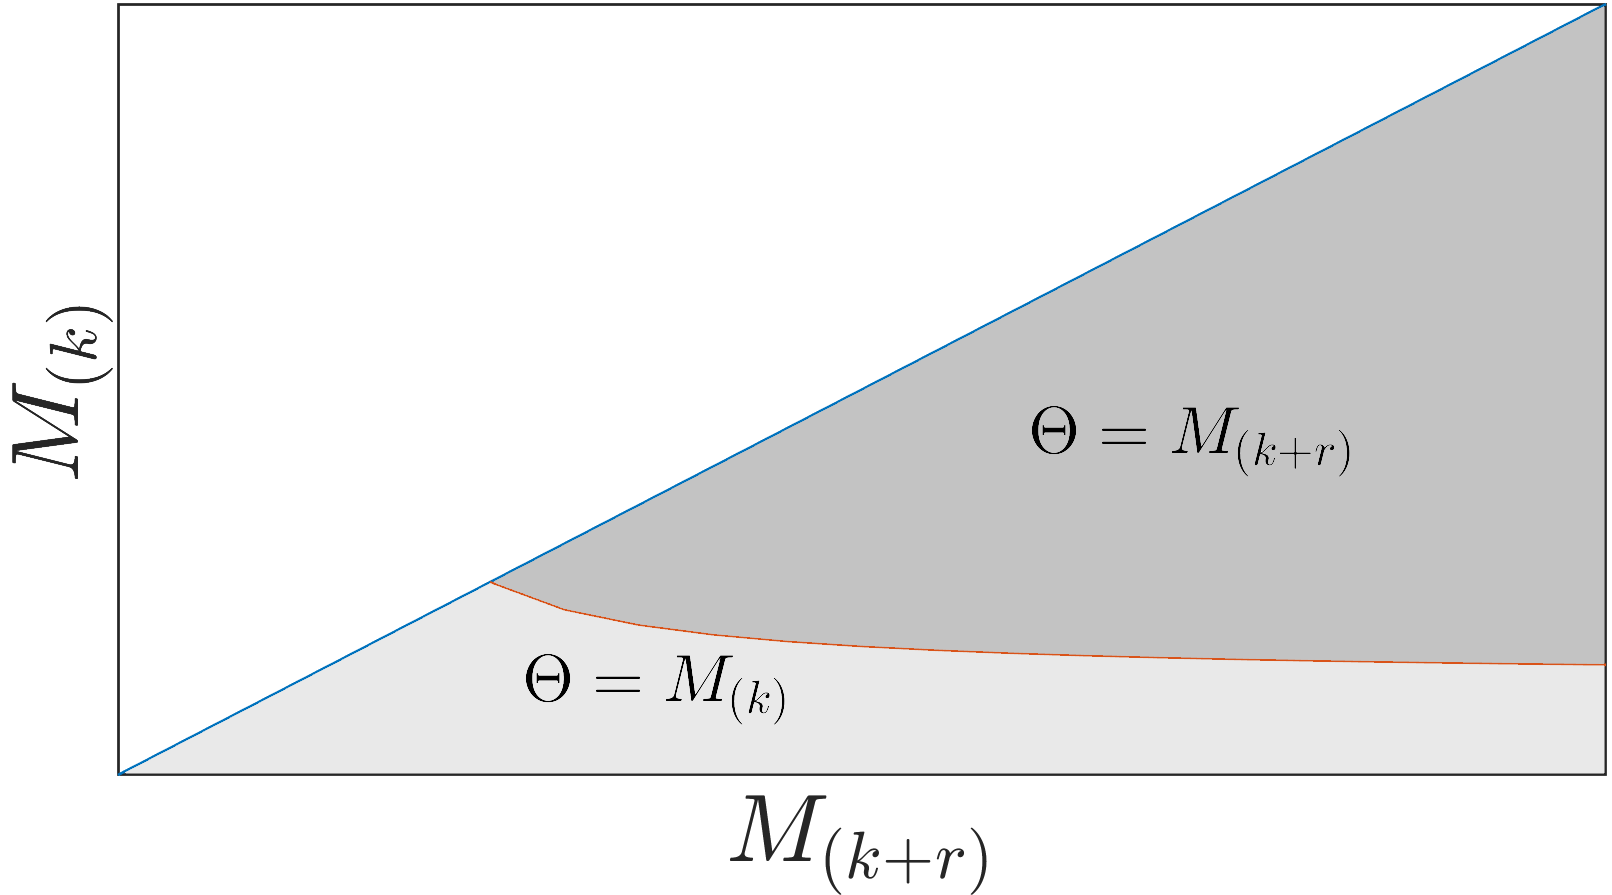
\includegraphics[width=0.38\textwidth]{graphics/fast-concurrent/areaGraph.png}
        %\vspace{-0.2in}
    \end{center}
    \caption{Areas of $M_{(k)}$ and $M_{(k+r)}$. In the dark gray 
    ${\mathcal{A}}_s$ induces $\Theta=M_{(k+r)}$, and in the light gray, $\Theta=M_{(k)}$. The white
    area is not feasible.} %\vspace{-0.1in}
    \label{fc-fig:areaGraph}
%\end{wrapfigure}
\end{figure}

Consider an adversary $\mathcal{A}$ whose estimate is a random variable $e_{\mathcal{A}}$,
characterized by the probability density function $f_{e_{\mathcal{A}}}$.
The expectation of $e_{\mathcal{A}}$ is not necessarily $n$, and so the relative standard error needs to be computed as the error from the desired estimate, $n$, rather than from the expectation. This can be done using the following formula:
\[
    (\textit{RSE}[e_{\mathcal{A}}])^2 = \frac{1}{n^2} \Int_{-\infty}^{\infty} (e - n)^2 \cdot f_{e_{\mathcal{A}}}(e) \,de 
\]
We prove
the following bound:
%Lemma~\ref{fc-lemma:theta-adversary-bound} in the supplementary material Section~\ref{fc-ssec:theta-error-bounds} proves the following bound:
\begin{align*}
    \textit{RSE}[e_{\mathcal{A}}] \leq \sqrt{\frac{\sigma^2(e_{\mathcal{A}})}{n^2}} + \sqrt{\frac{(E[e_{\mathcal{A}}] - n)^2}{n^2}}.
\end{align*}

\begin{lemma}
    The RSE of $e_{\mathcal{A}}$ satisfies the inequality 
    $\textit{RSE}[e_{\mathcal{A}}] \leq \sqrt{\frac{\sigma^2(e_{\mathcal{A}})}{n^2}} + \sqrt{\frac{(E[e_{\mathcal{A}}] - n)^2}{n^2}}$.
    \label{fc-lemma:theta-adversary-bound}
\end{lemma}
\begin{proof}
    \begin{align*}
    \begin{split}
    (\textit{RSE}[e_{\mathcal{A}}])^2 &= \frac{1}{n^2} \Int_{-\infty}^{\infty} (e - n)^2 \cdot f_{e_{\mathcal{A}}}(e) \,de \\
    &= \frac{1}{n^2} \Int_{-\infty}^{\infty} (e - E[e_{\mathcal{A}}] + E[e_{\mathcal{A}}] - n)^2 \cdot f_{e_{\mathcal{A}}}(e) \,de \\
    &\leq \frac{1}{n^2} \Int_{-\infty}^{\infty} \left((e - E[e_{\mathcal{A}}])^2 + (E[e_{\mathcal{A}}] - n)^2 \right)\cdot f_{e_{\mathcal{A}}}(e) \,de \\
    &= \frac{\sigma^2(e_{\mathcal{A}}) + (E[e_{\mathcal{A}}] - n)^2}{n^2} \\
    \text{RSE}[e_{\mathcal{A}}] &\leq \sqrt{\frac{\sigma^2(e_{\mathcal{A}})}{n^2}} + \sqrt{\frac{(E[e_{\mathcal{A}}] - n)^2}{n^2}}
    \end{split}
    \end{align*}
\end{proof}

\paragraph{Strong adversary ${\mathcal{A}}_s$} The strong adversary knows the coin flips in advance, and thus chooses
$j$ to be $g(0, r)$, where $g$ is the
choice that maximizes the error:
\begin{align*}
    g(j_1, j_2) \triangleq \argmax_{j \in \left\{j_1, j_2\right\}} \abs{\frac{k-1}{M_{(k+j)}} - n}.
\end{align*} 

\begin{figure}[b]
%\begin{wrapfigure}{l}{0.4\textwidth}
    \begin{center}
        %\vspace{-0.2in}
        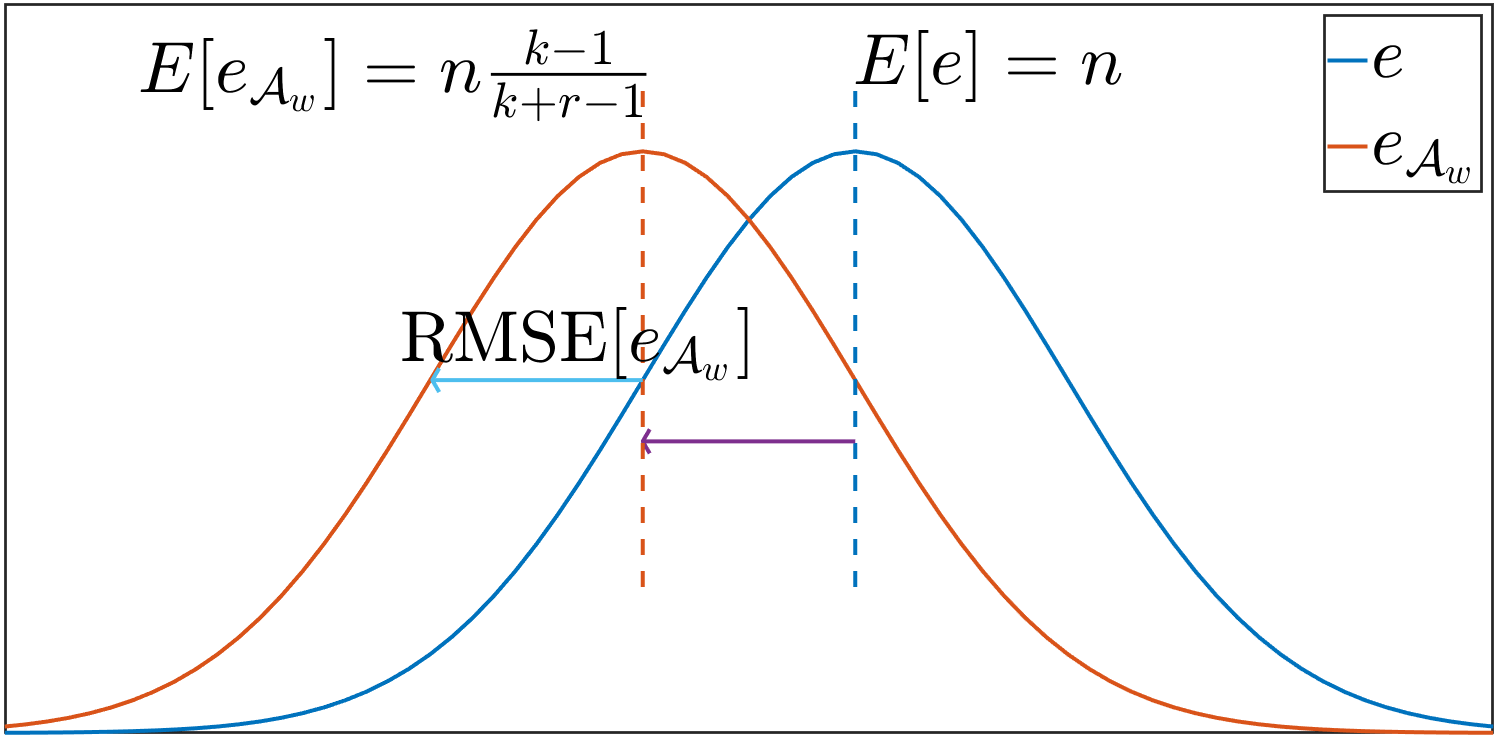
\includegraphics[width=0.39\textwidth]{graphics/fast-concurrent/thetaGraph.png}
        %\vspace{-0.2in}
    \end{center}
    \caption{Distribution of estimators $e$ and $e_{{\mathcal{A}}_w}$. The RSE of $e_{{\mathcal{A}}_w}$ with regards to $n$ is bounded
    by the relative bias plus the RMSE of $e_{{\mathcal{A}}_w}$.}%\vspace{-0.2in}}
    \label{fc-fig:thetaGraph}
%\end{wrapfigure}
\end{figure}

Recall the the ${\mathcal{A}}_s$ knows the oracles coin
flips, therefore knows $M_{(k)}$ and $M_{(k+r)}$, and chooses $M^r_{(k)}$ accordingly. Therefore, our analysis
is on the order statistics of the full stream, as it is this that the adversary sees. From order statistics, the joint probability density
function of $M_{(k)}, M_{(k+r)}$ is:
\begin{align*}
f_{M_{(k)},M_{(k+r)}}(m_k,m_{k+r}) = n!\frac{m_k^{k-1}}{(k-1)!} \frac{(m_{k+r}-m_k)^{r-1}}{(r-1)!}\frac{(1-m_{k+r})^{n-(k+r)}}{(n-(k+r))!}.
\end{align*}

The expectation of $e_{{\mathcal{A}}_s}$ and $e_{{\mathcal{A}}_s}^2$ can be computed as follows:
\begin{equation}
    \begin{split}
    E[e_{{\mathcal{A}}_s}] = \Int_{0}^{1} \Int_{0}^{m_{k+r}} e_{{\mathcal{A}}_s} \cdot f_{M_{(k)},M_{(k+r)}}(m_k,m_{k+r}) \,dm_{k}\,dm_{k+r} \\
    E[e_{{\mathcal{A}}_s}^2] = \Int_{0}^{1} \Int_{0}^{m_{k+r}} \left[e_{{\mathcal{A}}_s} \right] ^2 \cdot f_{M_{(k)},M_{(k+r)}}(m_k,m_{k+r}) \,dm_{k}\,dm_{k+r}
    \end{split}
    \label{fc-eq:strong-expectation}
\end{equation}
Finally, the RSE of $e_{{\mathcal{A}}_s}$ is derived from the standard error of $e_{{\mathcal{A}}_s}$:
\begin{equation}
    \begin{split}
    \text{RSE}[e_{{\mathcal{A}}_s}]^2 &= \frac{1}{n^2}\Int_{0}^{1} \Int_{0}^{m_{k+r}} \left( e_{{\mathcal{A}}_s} - n \right)^2 \cdot f_{M_{(k)},M_{(k+r)}}(m_k,m_{k+r}) \,dm_{k}\,dm_{k+r} \\
    &= \frac{1}{n^2} \Int_{0}^{1} \Int_{0}^{m_{k+r}} \left( e_{{\mathcal{A}}_s} -E[e_{{\mathcal{A}}_s}] + E[e_{{\mathcal{A}}_s}] - n \right)^2 \cdot f_{M_{(k)},M_{(k+r)}}(m_k,m_{k+r}) \,dm_{k}\,dm_{k+r} \\
    &\leq \frac{1}{n^2} \left(\sigma^2(e_{{\mathcal{A}}_s}) + (e_{{\mathcal{A}}_s} - n)^2 \right)\\
    \text{RSE}[e_{{\mathcal{A}}_s}] &\leq \sqrt{\frac{\sigma^2(e_{{\mathcal{A}}_s}) + (e_{{\mathcal{A}}_s} - n)^2}{n^2}} \\
    &\leq \sqrt{\frac{\sigma^2(e_{{\mathcal{A}}_s})}{n^2}} + \sqrt{\frac{(e_{{\mathcal{A}}_s} - n)^2}{n^2}}
    \end{split}
    \label{fc-eq:strong-se-bound}
\end{equation}

In Figure~\ref{fc-fig:areaGraph} we plot the regions where $g$ equals $0$
and $g$ equals $r$, based on their possible combinations of values. The estimate
induced by ${\mathcal{A}}_s$ is $e_{{\mathcal{A}}_s} \triangleq \frac{k-1}{M_{(k+g(0,r))}}$. The expectation
and standard error of $e_{{\mathcal{A}}_s}$ are calculated by integrating over the gray areas
in Figure~\ref{fc-fig:areaGraph} using their joint probability function from order statistics. %In the full paper~\cite{rinberg2019fast} we give
Equations \ref{fc-eq:strong-expectation} and \ref{fc-eq:strong-se-bound} give
the formulas for the expected estimate and its RSE bound, respectively. We do not have
closed-form bounds for these equations. Example numerical results, computed based on Equation~\ref{fc-eq:strong-se-bound}, are
shown in Table~\ref{fc-table:Theta-Error-Summary}.

\paragraph{Weak adversary ${\mathcal{A}}_w$} Not knowing the coin flips, ${\mathcal{A}}_w$ chooses $j$
that maximizes the expected error for a random hash function:
$E[n-est(M^r_{(k)})]=E[n-est(M_{(k+j)})]=n-n\frac{k-1}{k+j-1}$. Obviously this
is maximized for $j=r$. The orange curve in Figure~\ref{fc-fig:thetaGraph} depicts
the distribution of $e_{{\mathcal{A}}_w}$, and the distribution of $e$ is shown in blue.

Recall that ${\mathcal{A}}_w$ always hides $r$ elements smaller than $\Theta$, thus
forcing $M^r_{(k)}=M_{(k+r)}$. Here too our analysis is on the order statistics for the full stream, as this is what the adversary sees.
The expectation of $e_{{\mathcal{A}}_w}$ and $e_{{\mathcal{A}}_w}^2$ is computed using well known equations from order statistics:
\begin{align*}
    E[e_{{\mathcal{A}}_w}]&=E\left[ \frac{k-1}{M_{(k+r)}} \right]=n\frac{k-1}{k+r-1} \\
    E[e_{{\mathcal{A}}_w}^2]&=(k-1)^2\frac{n(n-1)}{(k+r-2)(k+r-1)} \\
    \sigma^2[e_{{\mathcal{A}}_w}] &= E[e_{{\mathcal{A}}_w}^2] - E[e_{{\mathcal{A}}_w}]^2 \\
    &=(k-1)^2\frac{n(n-1)}{(k+r-2)(k+r-1)} - \left(n\frac{k-1}{k+r-1} \right)^2 \\
    &< \frac{n(k-1)^2}{k+r-1}\left[\frac{n}{(k+r-2)(k+r-1)}\right] \\
    \sigma^2[e_{{\mathcal{A}}_w}] &< \frac{n^2}{k+r-2}
\end{align*}

We derive the following equation:
\begin{equation}
    \sqrt{\frac{\sigma^2[e_{{\mathcal{A}}_w}]}{E[e_{{\mathcal{A}}_w}]}}<\frac{1}{k-2}
    \label{fc-eq:ss-rse}
\end{equation}

Finally, the RSE of $e_{{\mathcal{A}}_w}$ is derived from the standard error of $e_{{\mathcal{A}}_w}$, and as $E[e_{{\mathcal{A}}_w}] < n$,
and using the same ``trick'' as in Equation~\ref{fc-eq:strong-se-bound}:
\begin{align*}
    \text{RSE}[e_{{\mathcal{A}}_w}]^2 &= \frac{1}{n^2}\Int_{0}^{1} \left( e_{{\mathcal{A}}_w} - n \right)^2 \cdot f_{M_{(k+r)}}(m_{k+r}) \,dm_{k+r} \\
    &< \frac{1}{n^2} \left(\sigma^2(e_{{\mathcal{A}}_w}) + (E[e_{{\mathcal{A}}_w}] - n)^2 \right)\\
    \text{RSE}[e_{{\mathcal{A}}_w}] &< \sqrt{\frac{\sigma^2(e_{{\mathcal{A}}_w})}{E[e_{{\mathcal{A}}_w}]^2}} + \sqrt{\frac{(E[e_{{\mathcal{A}}_w}] - n)^2}{n^2}}
\end{align*}

Using Equation~\ref{fc-eq:ss-rse}:
\begin{equation}
    \text{RSE}[e_{{\mathcal{A}}_w}] < \sqrt{\frac{1}{k-2}} + \frac{r}{k-2}
    \label{fc-eq:theta-rse-weak-bound}
\end{equation}

%In the full paper~\cite{rinberg2019fast},
%In Equation~\ref{fc-eq:theta-rse-weak-bound}% in the supplementary material Section~\ref{fc-ssec:theta-error-bounds} 
We have shown that the RSE
is bounded by $\sqrt{\frac{1}{k-2}} + \frac{r}{k-2}$ for ${{\mathcal{A}}}_w$.
Thus, whenever $r$ is at most $\sqrt{k-2}$, the RSE of the relaxed
$\Theta$ sketch is coarsely bounded by
twice that of the sequential one. And in case $k \gg r$, the addition to the $RSE$ is negligible.

\subsection{Error bounds for PAC sketches}

We now provide a generic analysis, considering a PAC sketch as a black box. 
Section~\ref{fc-ssec:quantiles-error-analysis} studies quantiles sketches, and 	
in Section~\ref{fc-ssec:pac-unique}, we study PAC sketches estimating the number of unique elements in a stream, e.g., HyperLogLog. 
In both cases, we show that if the sequential sketch's error bound is $\epsilon$, then 
the error of an $r$-relaxed sketch over a stream of size $n$ is bounded by $\epsilon+\frac{r \epsilon}{n}+\frac{r}{n}$. 
This expression tends to  $\epsilon$ as the stream sizes grows to infinity, but may be substantially larger for small streams. 
A system designer can use this formula to determine the adaptation point so that the error is never above a desired threshold. 


\subsubsection{Quantiles error bounds}
\label{fc-ssec:quantiles-error-analysis}

%\begin{wraptable}{c}{0pt}
%    \begin{tabular}{c|ccc}
%    Quantile        & Sequential                                   & Weak adversary ${\mathcal{A}}_w$ \\[5pt]
%    \hline
%    $\phi \leq 0.5$ & $\phi n \pm \epsilon n$ & $\phi n + (1-\phi)r \pm \epsilon(n - r)$ \\[5pt]
%    $\phi > 0.5$    & $\phi n \pm \epsilon n$ & $\phi n -\phi r \pm \epsilon(n - r)$
%    \end{tabular}
%    \caption{Quantiles sketch: Result range with probability $1-\delta$, for sequential sketch and $r$-relaxation with weak adversary,
%    and $\epsilon_r=\epsilon - \frac{r \epsilon}{n} + \frac{r}{n}$.}
%    \label{fc-table:Quantiles-Error-Summary}
%\end{wraptable}

\iffalse
\begin{wraptable}{c}{0pt}
    \begin{tabular}{c|ccc}
    Quantile        & Sequential                                   & Weak adversary ${\mathcal{A}}_w$ \\[5pt]
    \hline
    $\phi $ & $\phi n \pm \epsilon n$ & $\phi n \pm \left(\epsilon - \frac{r \epsilon}{n} + \frac{r}{n}\right) n$ 
    \end{tabular}
    \caption{Quantiles sketch: Result range with probability $1-\delta$, for sequential sketch and $r$-relaxation with weak adversary,
    and $\epsilon_r=\epsilon - \frac{r \epsilon}{n} + \frac{r}{n}$.}
    \label{fc-table:Quantiles-Error-Summary}
\end{wraptable}
\fi

We now analyze the error for any implementation of the sequential Quantiles sketch, provided that the sketch is
\emph{PAC}, meaning that a query for quantile $\phi$
returns an element whose rank is between $(\phi-\epsilon)n$ and $(\phi+\epsilon)n$ with 
probability at least $1-\delta$ for some parameters $\epsilon$ and $\delta$. We show that the $r$-relaxation of
such a sketch returns an element whose rank is in the range $(\phi \pm\epsilon_r)n$ with probability at
least $1-\delta$ for $\epsilon_r=\epsilon - \frac{r \epsilon}{n} + \frac{r}{n}$.

Although the desired summary is order agnostic here too, Quantiles sketch implementations (e.g., \cite{agarwal2013mergeable})
are sensitive to the processing order. In this case, advance knowledge of the coin flips can increase the error
already in the sequential sketch. Therefore, we do not consider a strong adversary, but rather discuss only the weak one.
Note that the weak adversary attempts to maximize $\epsilon_r$.

Consider an adversary that knows $\phi$ and chooses to hide
$i$ elements below the $\phi$ quantile and $j$ elements above it, such that $0\leq i+j\leq r$. The rank of the element
returned by the query among the $n-(i+j)$ remaining elements is in the range 
$\phi(n-(i+j)) \pm \epsilon(n-(i+j))$.
There are $i$ elements below this quantile that are missed, and therefore its rank in the original stream is in the range:
\begin{equation}
    \left[ (\phi-\epsilon)(n-(i+j)) + i , (\phi+\epsilon)(n-(i+j)) + i \right].
    \label{fc-eq:rank-range}
\end{equation}

This can be rewritten as:
\begin{equation}
\begin{split}
    [\phi n - (\phi j - (1-\phi)i+\epsilon(n-(i+j))), \\
    \phi n + ((1-\phi)i - \phi j +\epsilon(n-(i+j))) ] 
\end{split}
    \label{fc-eq:rank-range-2}
\end{equation}

Note that this interval is symmetric around $\phi(n-(i+j)) + i$.
The adversary attempts to maximize the distance of the edges of this interval from the true rank,
(i.e., maximize $\epsilon_r$). The distance between the central points is:
\begin{align*}
    \abs{\phi n + (1-\phi)i - \phi j - \phi n}=\abs{(1-\phi)i - (\phi)j}.
\end{align*}
Given that $0\leq i+j\leq r$, we show that this expression is maximized
for $i+j=r$.
\begin{claim}
    Given $0\leq i,j$ such that $0\leq i+j\leq r$, the expression $\abs{(1-\phi)i - (\phi)j}$
    is maximized for $(i,j)=(x,y)$ such that $x+y=r$.
    \label{fc-claim:sum-r}
\end{claim}
\begin{proof}
    Assume by contradiction that the expression given in the claim is maximized for $(x,y)$ such that $x+y=r'<r$. Denote
    $r'=r-k$. We consider two cases for the expression $(1-\phi)i - (\phi)j$.

    If $(1-\phi)x - (\phi)y \geq 0$, then $(1-\phi)(x+k) - (\phi)y \geq (1-\phi)x - (\phi)y >0$. In this
    case denote $x'=x+k$ and $y'=y$.

    If $(1-\phi)x - (\phi)y < 0$, then $(1-\phi)x - (\phi)(y+k) \leq (1-\phi)x - (\phi)y < 0$. In this
    case denote $x'=x$ and $y'=y+k$.

    In both cases we found $(x',y')$ such that $x'+y'=r$ and the expression $\abs{(1-\phi)i - (\phi)j}$
    is maximized for $(i,j)=(x',y')$.
\end{proof}

%This is proven in Claim~\ref{fc-claim:sum-r} in the supplementary material Section~\ref{fc-ssec:quantiles-sketch-error-bounds}.
By substituting $j=r-i$ into the error formula, we get:
\begin{align*}
    \abs{(1-\phi)i - (\phi)(r-i)}=\abs{i - \phi r}.
\end{align*}
As $0\leq \phi \leq 1$, the following claim follows immediately:
\begin{claim}
    For $\phi \leq 0.5$ the adversary maximizes the distance by choosing $i=r$ (and therefore $j=0$)
    and for $\phi > 0.5$ the adversary maximizes the error by choosing $i=0$ (and therefore $j=r$).
    \label{fc-clm:quantiles-relaxation-choice}
\end{claim}

We begin by analyzing the range given in Equation~\ref{fc-eq:rank-range-2} for $0 \leq \phi \leq 0.5$.

\begin{claim}
    For $0 \leq \phi \leq 0.5$ and $i,j>0$ such that $0 \leq i+j \leq r$ and $\epsilon < 0.5$, then: (1) $(1-\phi)i-\phi j + \epsilon(n-(i+j)) \leq (1-\phi) r + \epsilon(n-r)$,
    and (2) $\phi j - (1-\phi)i + \epsilon(n-(i+j)) \leq (1-\phi) r + \epsilon(n-r)$.
    \label{fc-clm:quantiles-bottom-half}
\end{claim}
\begin{proof}
    As $\phi \leq 0.5$, and $\epsilon \ll 0.5$ then $1-\phi-\epsilon > 0$. As $0 \leq i+j \leq r$, then $i \leq r$.
    \begin{align}
        f(i,j)&=(1-\phi)i-\phi j + \epsilon(n-(i+j)) \leq (1-\phi)i + \epsilon(n-i) \leq (1-\phi-\epsilon)i +\epsilon n \\
        &\leq (1-\phi-\epsilon)r +\epsilon n = (1-\phi)r+\epsilon(n-r) = f(r,0)
    \end{align}

    As $\phi \leq 0.5$, then $\phi \leq 1-\phi$, and as As $0 \leq i+j \leq r$, then $i \leq r$
    \begin{align}
        \phi j - (1-\phi)i + \epsilon(n-(i+j)) \leq (1-\phi )j +\epsilon (n-j)  \leq (1-\phi) r + \epsilon (n-r)
    \end{align}
\end{proof}


We next analyze the same range for $0.5 < \phi \leq 1$.

\begin{claim}
    For $0.5 < \phi \leq 1$ and $i,j>0$ such that $0 \leq i+j \leq r$ and $\epsilon < 0.5$, then: (1) $\phi i - (1-\phi)j + \epsilon(n-(i+j)) \leq \phi r + \epsilon(n-r)$, 
    and (2) $(1-\phi)i - \phi j + \epsilon(n-(i+j)) \leq \phi r + \epsilon(n-r)$.
    \label{fc-clm:quantiles-top-half}
\end{claim}
\begin{proof}
    As $\phi > 0.5$, and $\epsilon \ll 0.5$ then $\phi-\epsilon > 0$. As $0 \leq i+j \leq r$, then $i \leq r$.
    \begin{align}
        f(i,j)=\phi i - (1-\phi)j + \epsilon(n-(i+j)) \leq \phi i +\epsilon (n-i) \leq (\phi - \epsilon)i + \epsilon n \leq \phi r + \epsilon(n-r) = f(r,0)
    \end{align}

    As $\phi > 0.5$, then $(1-\phi) \leq \phi$, and as As $0 \leq i+j \leq r$, then $i \leq r$
    \begin{align}
        (1-\phi)i - \phi j + \epsilon(n-(i+j)) \leq \phi i + \epsilon (n-i) \leq \phi r + \epsilon(n-r)
    \end{align}
\end{proof}

Putting the two claims together we get:

\begin{claim}
    For $0 \leq \phi \leq 1$ and $i,j>0$ such that $0 \leq i+j \leq r$ and $\epsilon \ll 0.5$, then: (1) $\phi i - (1-\phi)j + \epsilon(n-(i+j)) \leq r + \epsilon(n-r)$,
    and (2) $(1-\phi)i - \phi j + \epsilon(n-(i+j)) \leq r + \epsilon(n-r)$.
    \label{fc-clm:helper}
\end{claim}
\begin{proof}
    From Claim~\ref{fc-clm:quantiles-bottom-half}, for $0 \leq \phi \leq 0.5$ then both inequalities are bounded by $(1-\phi) r + \epsilon(n-r)$, and as $\phi \geq 0$ then
    $(1-\phi) r + \epsilon(n-r) \leq r + \epsilon(n-r)$.

    From Claim~\ref{fc-clm:quantiles-top-half}, for $0.5 < \phi \leq 1$ then both inequalities are bounded by $\phi r + \epsilon(n-r)$, and as $\phi \leq 1$ then
    $\phi r + \epsilon(n-r) \leq r + \epsilon(n-r)$.
\end{proof}

Finally, we prove a bound on the rank of the element returned. 
\begin{lemma}
    Given parameters $(\epsilon,\delta)$ if $\epsilon<0.5$, then the $r$-relaxed
    quantiles sketch returns an element whose rank is
    between $(\phi-\epsilon_r)n$ and $(\phi+\epsilon_r)n$ with probability at
    least $1-\delta$, where $\epsilon_r=\epsilon - \frac{r \epsilon}{n} + \frac{r}{n}$.
    \label{fc-lemma:quantiles-weak-adversary}
\end{lemma}
\begin{proof}
    Given parameters $(\epsilon,\delta)$, and given that the adversary hides $i$ elements below the
    $\phi$ quantile and $j$ elements above it, such that $0\leq i+j\leq r$, the rank of the element returned
    by the query is in the range given in Equation~\ref{fc-eq:rank-range-2} w.p. at least $1-\delta$:
    \begin{align*}
        \left[\phi n - (\phi j - (1-\phi)i+\epsilon(n-(i+j))), \phi n + ((1-\phi)i - \phi j +\epsilon(n-(i+j))) \right].
    \end{align*}

    From Claim~\ref{fc-clm:helper}, this range is contained within the range:
    \begin{align*}
        \left[\phi n - (r + \epsilon(n-r)), \phi n + (r + \epsilon(n-r)) \right].
    \end{align*}
    Which can be rewritten as the range $\left(\phi \pm \left(\epsilon - \frac{r \epsilon}{n} + \frac{r}{n}\right)\right)n$.
    Meaning the rank of the element returned is between $(\phi-\epsilon_r)n$ and $(\phi+\epsilon_r)n$ with probability at
    least $1-\delta$, where $\epsilon_r=\epsilon - \frac{r \epsilon}{n} + \frac{r}{n}$.
\end{proof}

%In the full paper~\cite{rinberg2019fast}, we
%In Lemma~\ref{fc-lemma:quantiles-weak-adversary} in the supplementary material Section~\ref{fc-sec:appendix-error-bounds} we
We have shown that the $r$-relaxed sketch returns an element whose rank is
%show that the $r$-relaxed sketch returns an element whose rank is
between $(\phi-\epsilon_r)n$ and $(\phi+\epsilon_r)n$ with probability at
least $1-\delta$, where $\epsilon_r=\epsilon - \frac{r \epsilon}{n} + \frac{r}{n}$. Thus
the impact of the relaxation diminishes as $n$ grows.
%The ranges are illustrated in Figure~\ref{fc-fig:quantiles-range}.

\subsubsection{Count unique elements error bounds}
\label{fc-ssec:pac-unique}

Finally, we consider the error of any implementation of a count unique elements sketch, provided
that the sketch is PAC. In this case, for a stream with $n$ unique elements, the query returns an estimate $e$ which is in between
$(1-\epsilon)n$ and $(1+\epsilon)n$ with probability at least $1-\delta$ for some parameters
$\epsilon$ and $\delta$. We show that the $r$-relaxation of such a sketch returns an estimate
is in the range $(1 \pm \epsilon_r)n$ with probability at least $1-\delta$
for $\epsilon_r=\epsilon+\frac{r \epsilon}{n}+\frac{r}{n}$.

As in a Quantiles sketch, advance knowledge of the coin flip can increase the
error already in the sequential sketch. Therefore, here too, we focus on a weak adversary.  
As above, the adversary hides either no
elements or $r$ elements. If the adversary hides $r$ elements, the estimate returned is in the range
$(1 \pm \epsilon)(n-r)$.

The adversary thus chooses whether to hide $r$ elements or not based on which estimate maximizes the
error $|n-e|$. In either case, with probability at least $1-\delta$ the estimate is between
$(1-\epsilon)(n-r)$ and $(1+\epsilon)n$. This range is contained in the range
$n\left(1 \pm \left(\epsilon+\frac{r \epsilon}{n}+\frac{r}{n}\right)\right)$. We can define
$\epsilon_r \triangleq \epsilon+\frac{r \epsilon}{n}+\frac{r}{n}$. Note that, as in the case of the
Quantiles sketch, here too, the impact of the relaxation diminishes as $n$ grows.

\section{\texorpdfstring{$\Theta$}{Theta} sketch evaluation}
\label{fc-sec:eval}

This section presents an evaluation of an implementation of our algorithm for the $\Theta$ sketch.
Section~\ref{fc-ssec:setup-and-methodology} presents the methodology for the analysis.
Section~\ref{fc-ssec:results} shows the results under different
workloads and scenarios. Finally, Section~\ref{fc-ssec:tradeoffs} discusses the tradeoff between
accuracy and throughput.

\subsection{Setup and methodology}
\label{fc-ssec:setup-and-methodology}

Our implementation~\cite{ConcurrentThetaImp} extends the code in Apache DataSketches~\cite{DataSketches}, a Java
open-source library of stochastic streaming algorithms. The $\Theta$ sketch there differs slightly
from the KMV $\Theta$ sketch we used as a running example, and is based on a HeapQuickSelectSketch family.
In this version, the sketch stores between $k$ and $2k$ items, whilst keeping $\Theta$ as the $k^{\text{th}}$
largest value. When the sketch is full, it is sorted and the largest $k$ values are discarded.

Concurrent $\Theta$ sketch is generally available in the Apache DataSketches
library since V0.13.0. The sequential implementation and the sketch at the core of the global sketch
in the concurrent implementation are the both \\ HeapQuickSelectSketch, which is the default sketch family.


We implement a limit for eager propagation as a function
of the configurable error parameter $\epsilon$; the function we use is $2 / \epsilon^2$. The local sketches define $b$
as a function of $k$, $\epsilon$, and $N$ (the number of writer threads) such that the error induced by
the relaxation when in the lazy propagation mode does not exceed $e$ using Equation~\ref{fc-eq:theta-rse-weak-bound}.
Thus the total error is bounded by $\max\{\epsilon + \frac{1}{\sqrt{k}}, \frac{2}{\sqrt{k}}\}$.

Eager propagation, as described in the pseudo-code, requires context switches incurring a high overhead. In the
implementation, either the local thread itself executes every update to the global sketch (equivalent to a
buffer size of 1) or lazily delegates updates to a background thread. While the sketch is in eager propagation
mode, the global sketch is protected by a shared boolean flag. When the sketch switches to estimate mode it
is guaranteed that no eager propagation gets through; instead local threads pass the buffer via lazy propagation.
This implementation ensures that: (a) local threads avoid costly context switches when the sketch is small, and (b)
lazy propagation by a background thread is done without synchronization.

Unless stated otherwise, we use k=4096, which is commonly used~\cite{DataSketches} for the $\Theta$ sketch.
The sequential sketch’s RSE with this buffer size is $0.031$ with a probability of at
least $0.95$. In the concurrent sketch, we chose to limit the error to $\epsilon = 0.04$ with the
same probability. Given a particular number of threads $N$, $b$ is derived according to
Equation~\ref{fc-eq:theta-rse-weak-bound} with $r = 2Nb$. Recall that the analysis in Section~\ref{fc-ssec:theta-analysis}
(including this equation) is
conditioned on the assumption that $n > k + r$. Therefore, if we would set the eager
adaptation threshold to $k+2Nb$, we would get the same error bound for any sketch size.
However, this is a conservative choice. We experiment with a threshold of $1250$,
and show that empirically, the error is reasonable with this choice. In general, this is
a configurable parameter, which can be used by system designers to navigate the tradeoff between
accuracy and performance.

%Unless otherwise stated, sketches are configured with $k=4096$, and $\epsilon=0.04$; thus the sketch swithces
%from eager propagation to lazy after $2/\epsilon^2=1250$ unique elements, and
%$b$ is set (by the implementation) to a value between $1$ and $5$ to accommodate the
%error bound.
Our first set of tests run on a 12-core Intel Xeon E5-2620 machine -- this machine is similar
to that which is used by production servers. For the scalability evaluation (shown in the introduction) we use a 32-core Intel Xeon
E5-4650 to get a large number of threads. Both machines have hyper-threading disabled, as it introduces
non-monotonic effects among threads sharing a core.

We focus on two workloads: (1) write-only -- updating a sketch with a stream of unique values; (2) mixed
read-write workload -- updating a sketch with background reads querying the number of unique values in
the stream. Background reads refer to dedicated threads that occasionally (with $1$ms pauses) execute a query.
These workloads simulate scenarios where updates are constantly streaming from
a feed or multiple feeds, while queries arrive at a lower rate.

To run the experiments we employ a multi-thread extension of the characterization
framework. This is the Apache DataSketch evaluation benchmark suite, which measures
both the speed and accuracy of the sketch. 

For measuring write throughput, the sketch is fed with a continuous data stream. The size of
the stream varies from 1 to 8M unique values. For each size $x$ we measure the time $t$ it takes to feed the
sketch $x$ unique values, and present it in term of throughput ($x/t$).
To minimize measurement noise, each point on the graph represents an average of
many trials. Small stream sizes tend to suffer more from measurement noise, so
the number of trials is very high (in the millions). As the stream size gets larger,
the number of trials gradually decreases down to 16 in the largest stream.
%The number of trials is very high
%($2^{18}$) for points at the low end of the graph. It gradually decreases as the size of the
%sketch increases. At the high end (at 8M values per trial) the number of trials is 16. This is because
%smaller stream sizes tend to suffer more from measurement noise.

Note that accuracy is measured relative to the number of unique elements ingested to the
sketch before a query in some linearization; because we cannot empirically deduce the
linearization point of a query that is run in parallel with updates, the metric is only
well-defined when the query is not concurrent to any update. Therefore, we measure
accuracy only in a single-thread environment, where we periodically interleave queries
with updates of the same thread. The accuracy with more threads can be extrapolated
from these measurements based on the theoretical analysis.

As in the performance evaluations, the $x$-axis represents the number of unique values fed into the sketch
by a single writing thread. For each size $x$, one trial logs the estimation result after feeding $x$
unique values to the sketch. In addition, it logs the Relative Error (RE) of the estimate, where
$\mathit{RE} = \mathit{MeasuredValue}/\mathit{TrueValue} - 1$. This trial is repeated 4K times,
logging all estimation and $\mathit{RE}$ results. The curves depict the mean and some
quantiles of the distributions of error measured at each $x$-axis point on the graph, including the median. 
This type of graph is called a ``pitchfork''.


\subsection{Results}
\label{fc-ssec:results}

\paragraph{Accuracy results}
Our first set of tests runs on a 12-core Intel Xeon E5-2620 machine. The accuracy results for the concurrent $\Theta$ sketch
without eager propagation are presented in Figure~\ref{fc-fig:accuracy}. There are two interesting phenomena worth noting.
First, it is interesting to see empirical evaluation reflecting the theoretical analysis presented in Section~\ref{fc-ssec:theta-analysis},
where the pitchfork is distorted towards underestimating the number of unique values. Specifically, the mean relative error is smaller
than $0$ (showing a tendency towards underestimating), and the relative error in all measured quantiles tends to be smaller
than the relative error of the sequential implementation.

Second, when the stream size is less than $2k$, $\Theta=1$ and the estimation is the number of values propagated to the
global sketch. If we forgo eager propagation, the number of values in the global sketch depends on the delay in propagation. The
smaller the sketch, the more significant the impact of the delay, and the mean error reaches as high as $94\%$ (the error in
the figure is capped at $10\%$). As the number of propagated values approaches $2k$, the delay in propagation is less significant, and
the mean error decreases. This excessive error is remedied by the eager propagation mechanism. The maximum error allowed by
the system is passed as a parameter to the concurrent sketch, and the global sketch uses eager propagation to stay within
the allowed error limit. Figure~\ref{fc-fig:accuracy-adaptive} depicts the accuracy results when applying eager
propagation. The figures are similar when the sketch begins lazy propagation, and the error stays within the $0.04$
limit as long as eager propagation is used.

\begin{figure*}[tb]
    \setlength{\abovecaptionskip}{0pt}
    \setlength{\belowcaptionskip}{0pt}
    \setlength\textfloatsep{0pt}
    \centering
    \begin{subfigure}{\columnwidth}\centering
    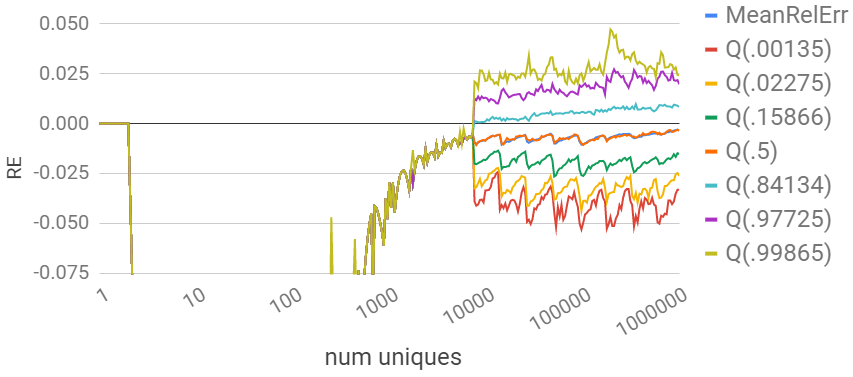
\includegraphics[width=\textwidth]{graphics/fast-concurrent/theta-accuracy.PNG}
    \caption{No eager propagation ($\epsilon=1.0$)}
    \label{fc-fig:accuracy}
    \end{subfigure}
    \begin{subfigure}{\columnwidth}\centering
    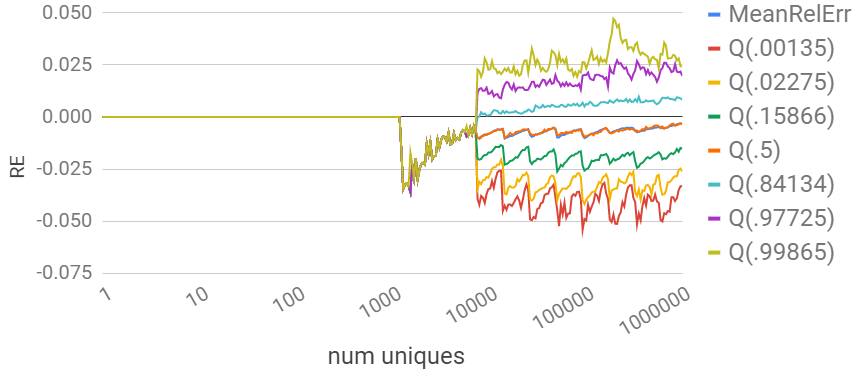
\includegraphics[width=\textwidth]{graphics/fast-concurrent/theta-accuracy-adaptive.PNG}
    \caption{With eager propagation, error bound defined by $\epsilon=0.04$}
    \label{fc-fig:accuracy-adaptive}
    \end{subfigure}
      \caption{Concurrent $\Theta$ measured quantiles vs RE, $k = 4096$.}
      \label{fc-fig:accuracy-res}
\end{figure*}

\paragraph{Write-only workload}
Figure~\ref{fc-fig:throughput:native} presents throughput measurements for a write-only workload. The results are shown in $\log \log$ scale.
Figure~\ref{fc-fig:throughput:large} zooms-in on the throughput of large streams. As explained in Section~\ref{fc-ssec:setup-and-methodology},
we compare the concurrent implementation to a lock-based approach. The number of threads in both implementations refers to the
number of worker threads; there can be arbitrarily many reader threads.

When considering large stream sizes, the concurrent implementation scales with the number of threads, peaking at
almost $300$M operations per second with $12$ threads. The performance of the lock-based implementation, on the other hand,
degrades as the contention on the lock increases.
%Its peak performance is $25$M operations per second with a single thread.
At the peak measured performance the single threaded concurrent $\Theta$ sketch outperforms the single
threaded lock based implementation by $12$x, and with $12$ threads by more than $45$x.
%Namely, with a single thread, the concurrent $\Theta$ sketch outperforms the lock-based implementation
%by $12$x, and with $12$ threads by more than $45$x. 

For small streams, wrapping a single thread with a lock is the most efficient method. Once the stream
contains more than $200$K unique values, using a concurrent sketch with $4$ or more local threads is more efficient.
The crossing point where a single local buffer is faster than the lock-based implementation is around $700$K unique values.
 
\begin{figure*}[tb]
\setlength{\abovecaptionskip}{0pt}
\setlength{\belowcaptionskip}{0pt}
\setlength\textfloatsep{0pt}
\centering
\begin{subfigure}{\columnwidth}\centering
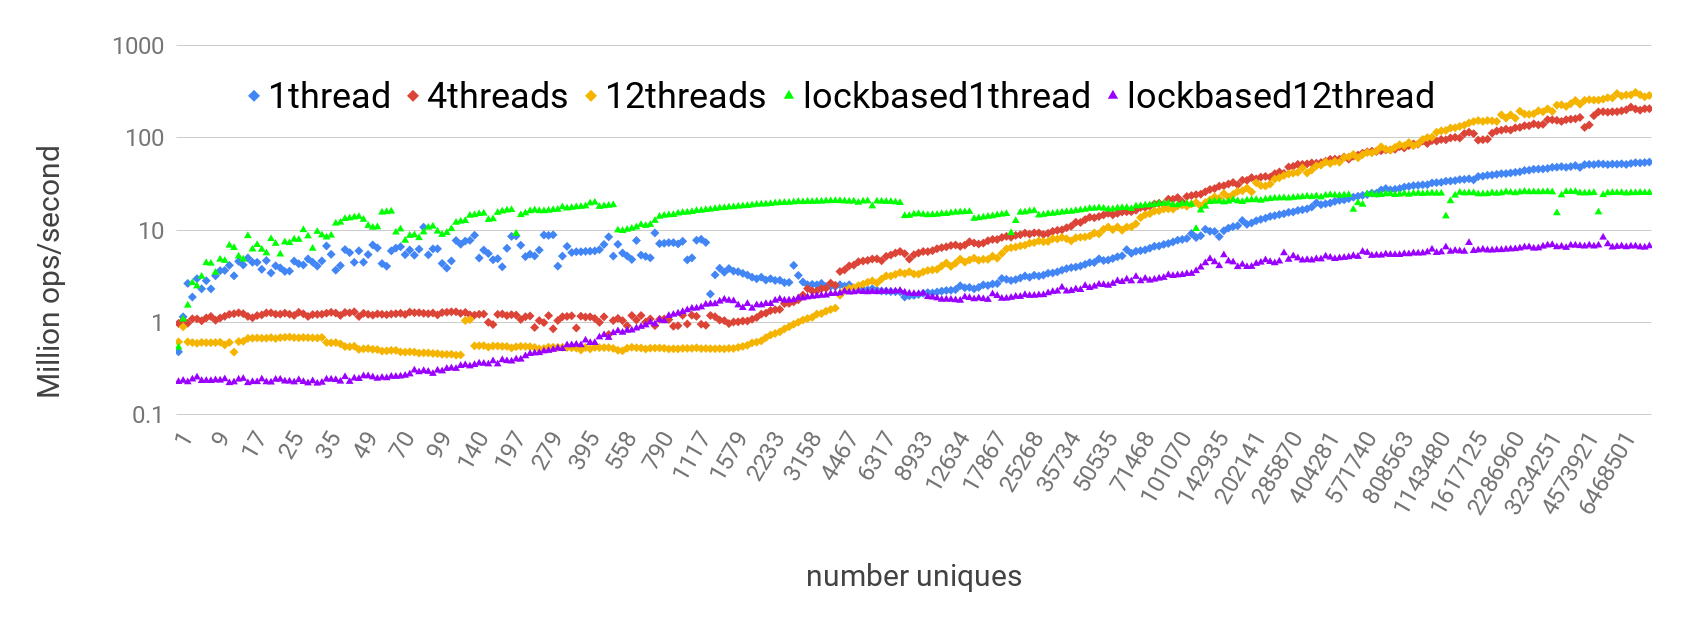
\includegraphics[width=\textwidth]{graphics/fast-concurrent/theta-write-only.png}
\caption{Throughput, loglog scale}
\label{fc-fig:throughput:native}
\end{subfigure}
\begin{subfigure}{\columnwidth}\centering
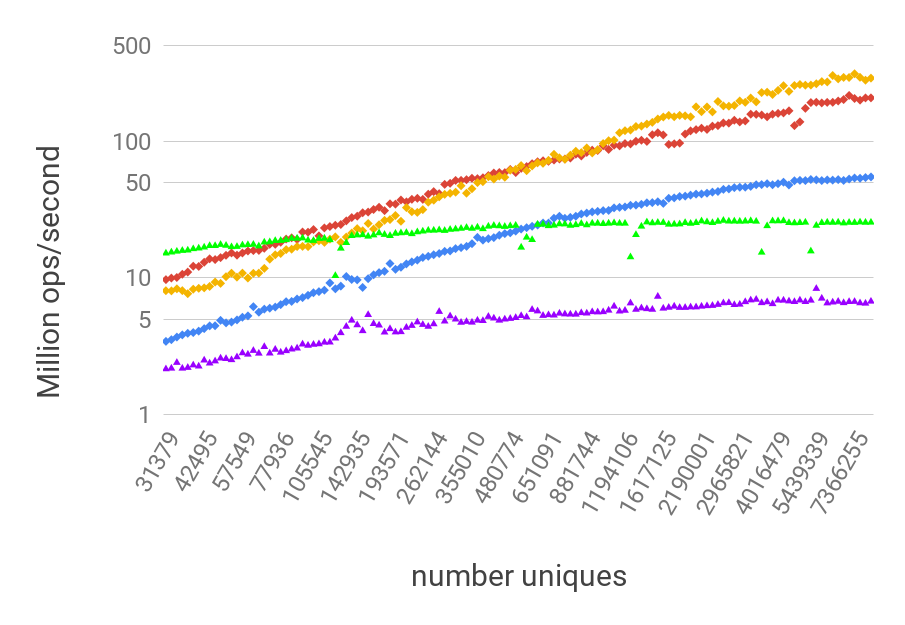
\includegraphics[width=\textwidth]{graphics/fast-concurrent/theta-write-only-zoomin.png}
\caption{Zooming-in on large sketches}
\label{fc-fig:throughput:large}
\end{subfigure}
  \caption{Write-only workload, $k = 4096$, $\epsilon=0.04$.}
  \label{fc-fig:throughput}
\end{figure*}


\paragraph{Mixed workload}
Figure~\ref{fc-fig:mixed-throughput} presents the throughput measurements
of a mixed read-write workload. We compare runs with a single updating thread and $2$
updating threads (and $10$ background reader threads).
Although we see similar trends as in the write-only workload, the effect of
background readers is more pronounced in the lock-based implementation than in the concurrent one;
this is expected as the reader threads compete for the same lock as the writers.
The peak throughput of a single writer thread in the concurrent implementation is $55$M ops/sec both with and
without background readers. The peak throughput of a single writer thread in the lock-based
implementation degrades from $25$M ops/sec without background reads to $23$M ops/sec with them; this is an almost $10$\% slowdown in performance.
Recall that in this scenario reads are infrequent, and so the degradation is not dramatic.

\begin{figure}[tb]
\setlength{\abovecaptionskip}{0pt}
\setlength{\belowcaptionskip}{0pt}
\setlength\textfloatsep{0pt}
	\centering
	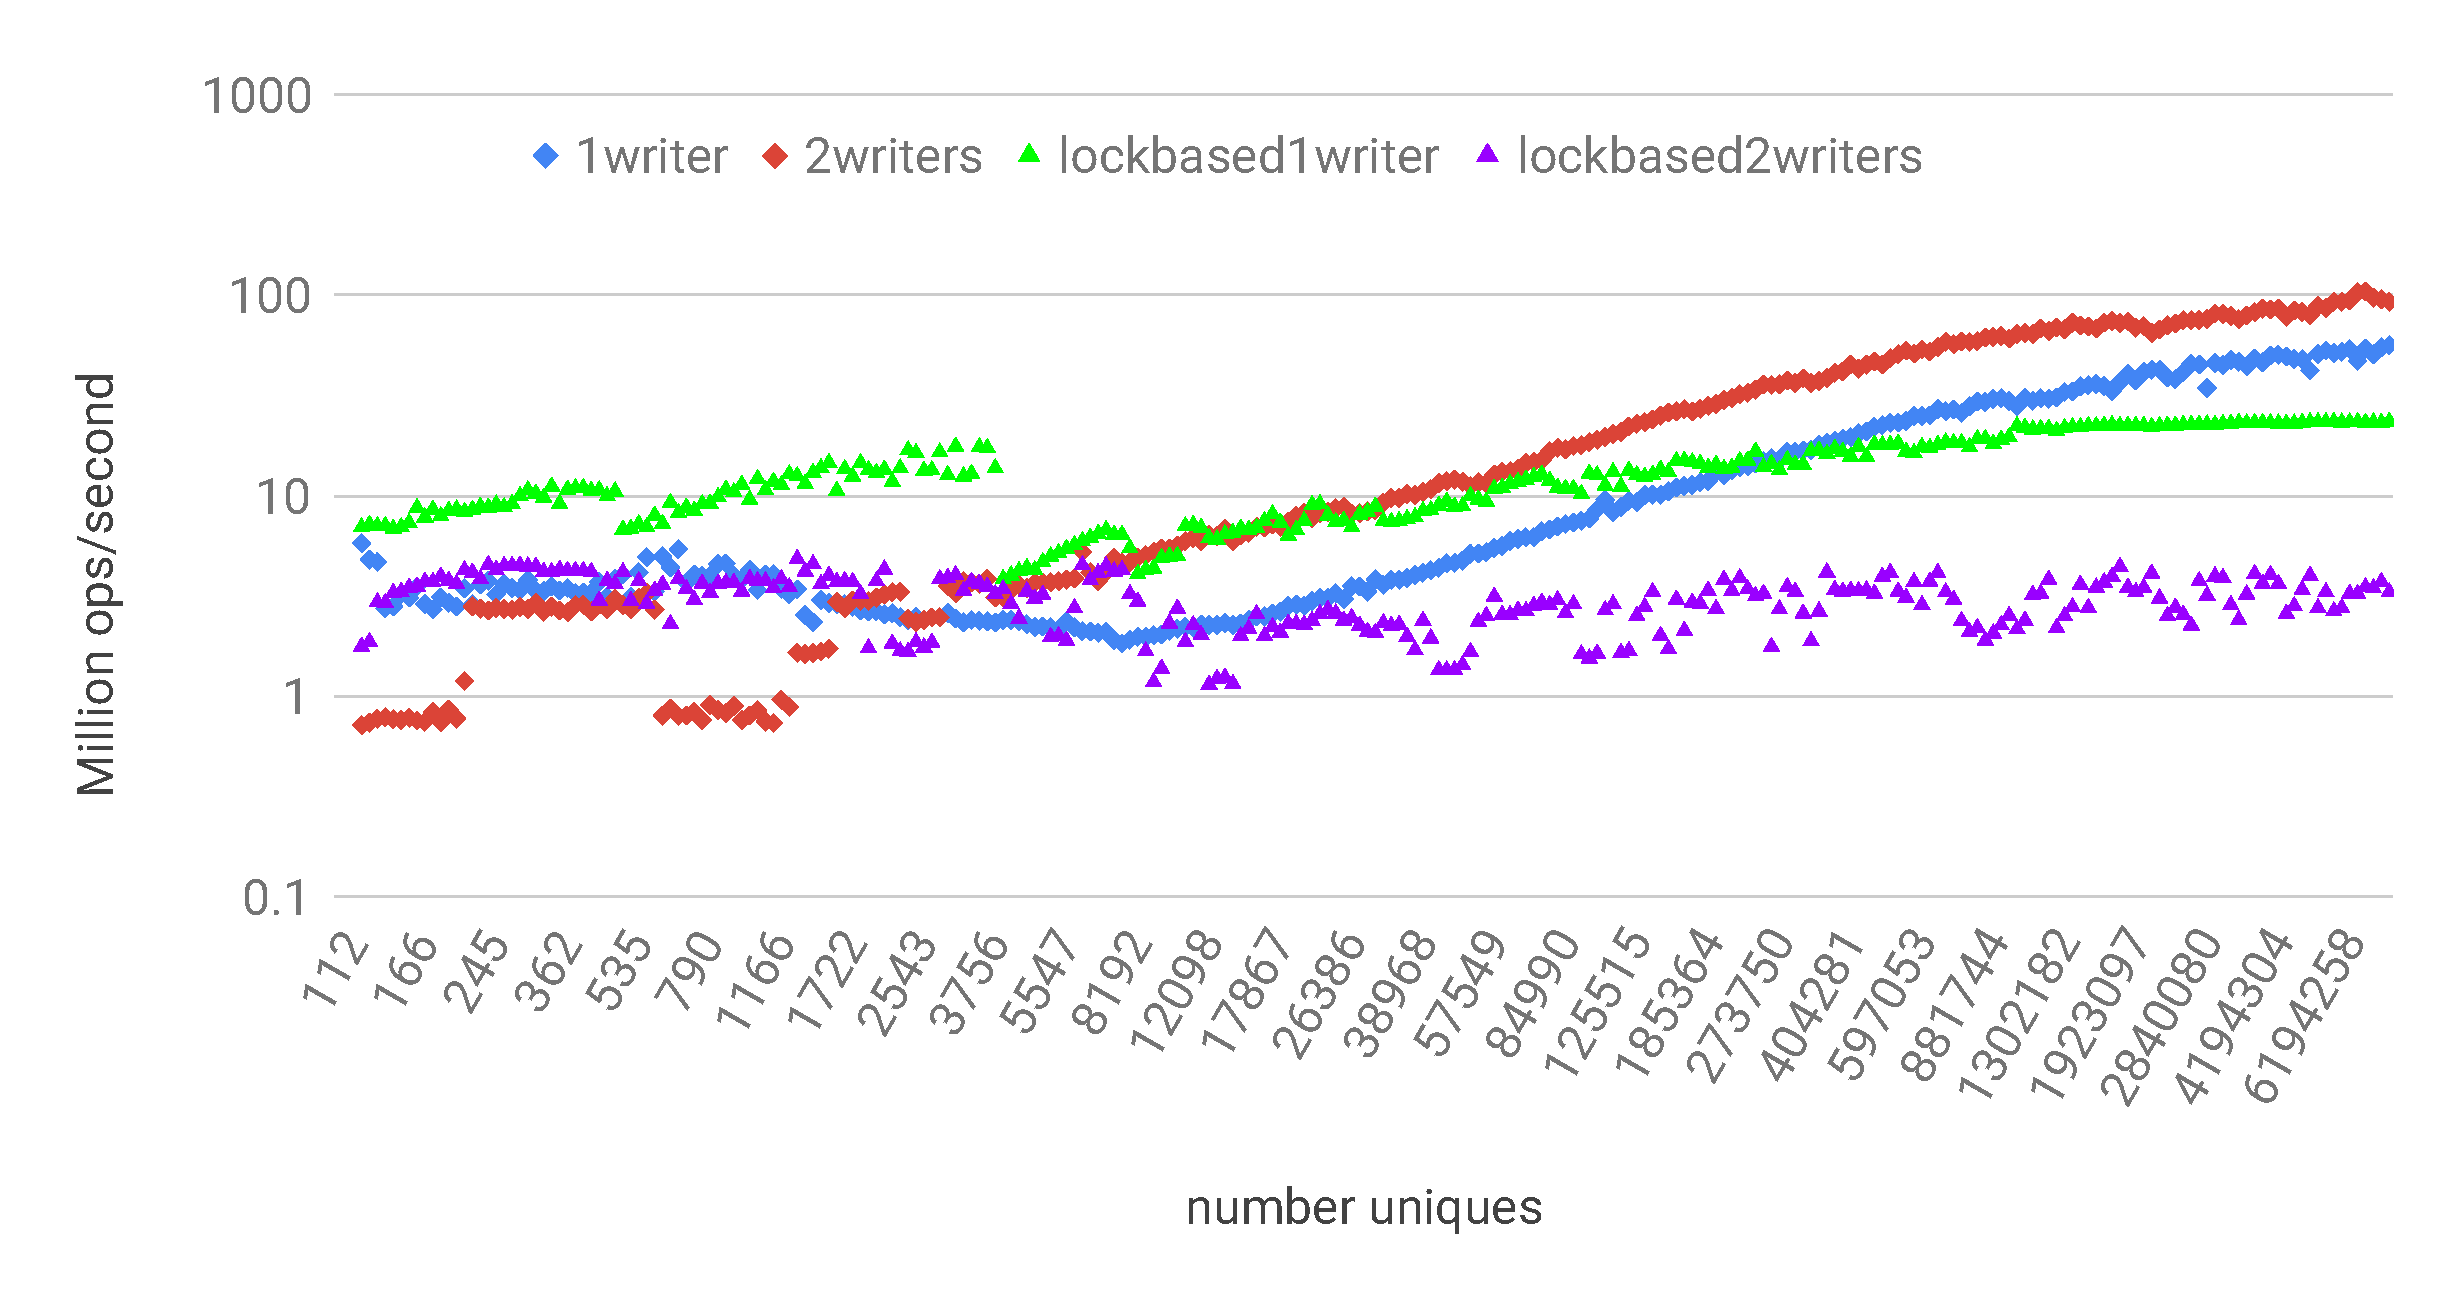
\includegraphics[width=\columnwidth]{graphics/fast-concurrent/theta-mixed.pdf}
	\caption{{Mixed workloads: writers with background reads, $k = 4096$, $\epsilon=0.04$.}}
	\label{fc-fig:mixed-throughput}
\end{figure}


\paragraph{Scalability results}
To provide a better scalability analysis, we aim to maximize the number of threads working on the
sketch. Therefore, we run this test on a larger machine -- we use a 32-core Xeon E5-4650 processors.
We ran an \emph{update-only} workload in which a sketch is built from a very large stream, repeating
each test 16 times.

In Figure~\ref{fc-fig:performance} (in the introduction) we compare the scalability
of our concurrent $\Theta$ sketch and the original sketch wrapped
with a read/write lock in an update-only workload, for $b=1$ and $k=4096$.
As expected, the lock-based sequential sketch does not scale, and
in fact it performs worse when accessed concurrently by many threads.
In contrast, our sketch achieves almost perfect scalability.
$\Theta$ quickly becomes small enough to allow filtering out most of the updates and so the
local buffers fill up slowly.


\subsection{Accuracy-throughput tradeoff}
\label{fc-ssec:tradeoffs}

The speedup achieved by eager propagation in small streams is presented in Figure~\ref{fc-fig:speedup}.
This is an additional advantage of eager propagation in small streams, beyond the accuracy benefit reported in Figure~\ref{fc-fig:accuracy-res}. 
The improvement is as high as $84$x for tiny sketches, and tapers off as the sketch grows.
The slowdown in performance when the sketch size exceeds $2k$ can be explained by the reduction
in the local buffer size (from $b=16$ to $b=5$), needed in order to accommodate for the required error bound.

\begin{figure}[tb]
\setlength{\abovecaptionskip}{0pt}
\setlength{\belowcaptionskip}{0pt}
\setlength\textfloatsep{0pt}
	\centering
	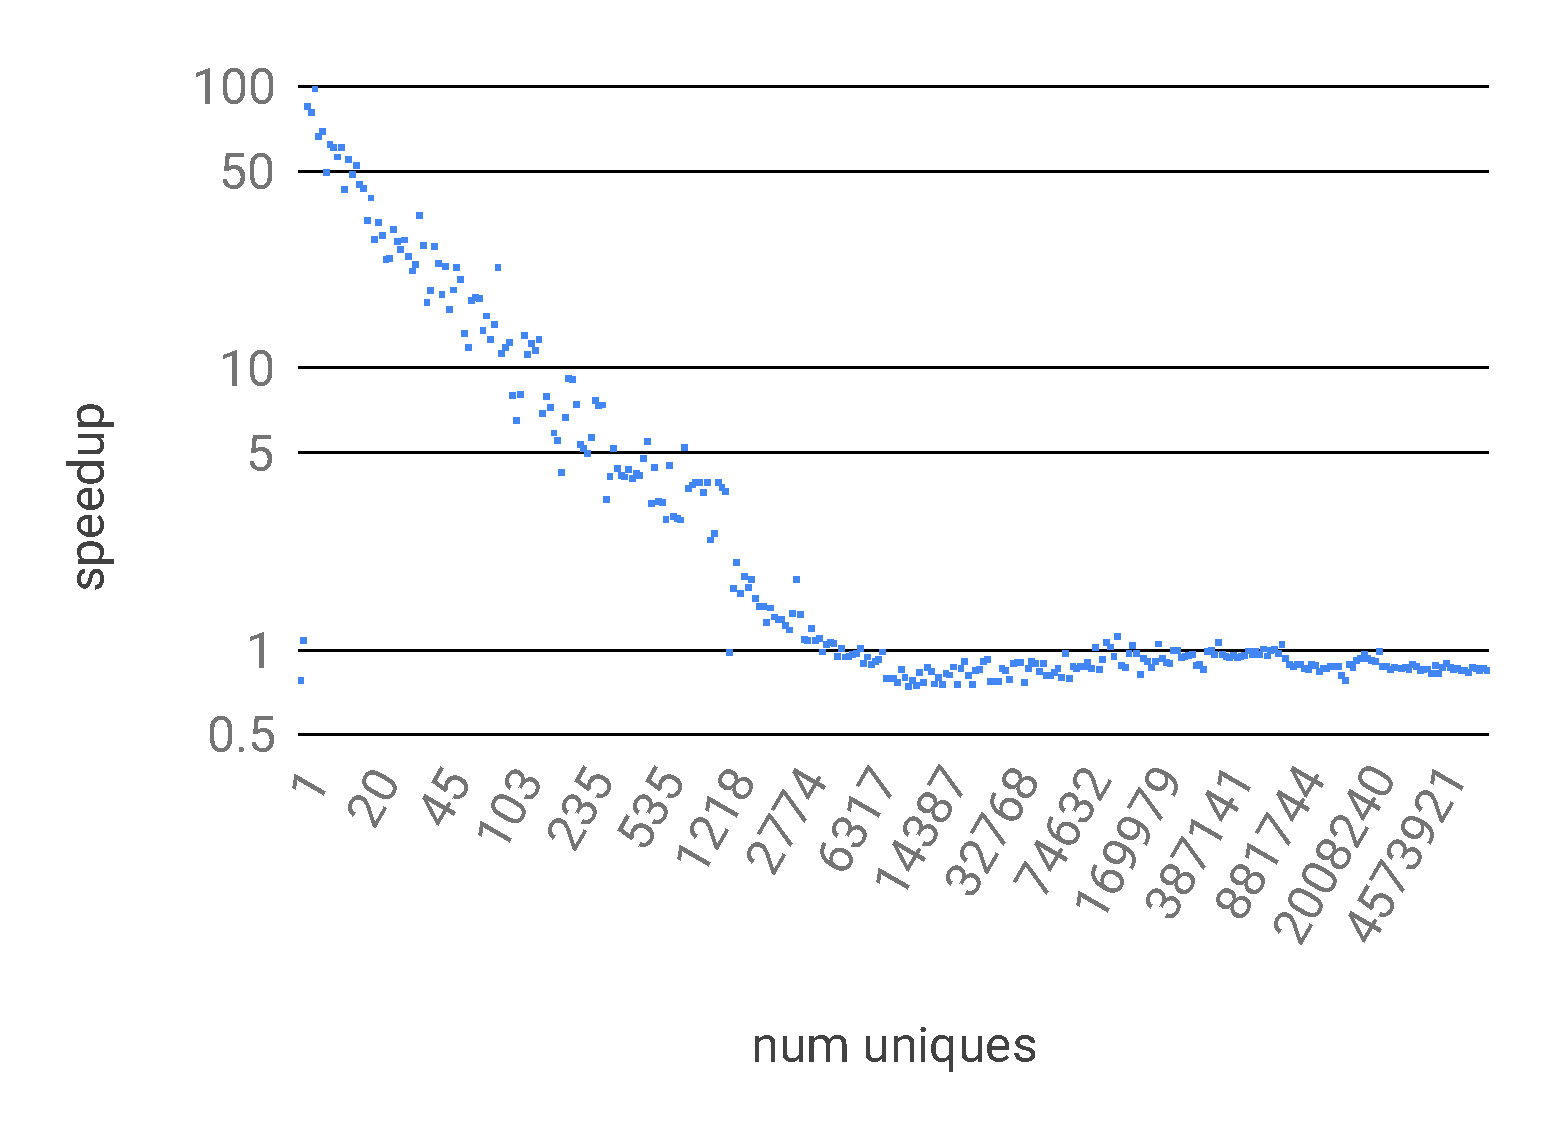
\includegraphics[width=\columnwidth]{graphics/fast-concurrent/eager-speedup.pdf}
	\caption{{Throughput speedup of eager ($\epsilon=0.04$) vs no-eager ($\epsilon=1.0$) propagation, $k = 4096$.}}
	\label{fc-fig:speedup}
\end{figure}


Next we discuss the impact of $k$.
One way to increase the throughput of the concurrent $\Theta$ sketch is by
increasing the size of the global sketch, namely increasing $k$. On the other hand,
this change also increases the error of the estimate.
Table~\ref{fc-tab:tradeoff} presents the tradeoffs between performance and accuracy.
Specifically, it presents the crossing-point, namely the smallest stream size for which the concurrent
implementation outperforms the lock-based implementation (both running a single thread). It further presents
the maximum values (across all stream sizes) of the median error and 99th percentile error for a variety of $k$ values.
The table shows that as the sketch promises a smaller error (by using a larger $k$), a larger stream size is needed to justify using
the concurrent sketch with all its overhead.

\begin{table}[htb]
\center{\small{
\begin{tabular}{lrrr}
\hline 
& thpt crossing point & mean error & error $Q=0.99$ \\
\hline 
$k=256$ &  15,000 &	0.16 & 0.27 \\
\hline 
$k=1024$ &  100,000 &	0.05 & 0.13 \\
\hline 
$k=4096$ & 700,000	& 0.03	& 0.05	\\ 
\hline 
\end{tabular}
}}
\caption{{Performance vs accuracy as a function of $k$.}}
\label{fc-tab:tradeoff}
\end{table}  




%\input{sections/appendixEvaluation.tex}
%\input{sections/Evaluation.tex}


\section{Conclusions}
\label{fc-sec:discussion}

Sketches are widely used by a range of applications
to process massive data streams and answer queries about them.
Library functions producing sketches
are optimized to be extremely fast, often digesting tens of millions of stream elements per second. 
We presented a generic algorithm for parallelizing such sketches and serving
queries in real-time; the algorithm is strongly linearizable with regards to relaxed semantics.
%\inred{We discussed the necessity of adapation for small streams, and how to implement such an adapation.}
We showed that the error bounds of two representative sketches,
$\Theta$ and Quantiles, do not increase drastically with such a relaxation. We also
implemented and evaluated the solution, showed it to be scalable {and accurate}, and integrated it into
the open-source Apache DataSketches library. While we analyzed only two sketches, future work
may leverage our framework for other sketches. Furthermore, it would be interesting to investigate
additional uses of the hint, for example, in order to dynamically adapt the size of the local buffers
and respective relaxation error.

\chapter{Intermediate Value Linearizability: A Quantitative Correctness Criterion}
\label{chap:ivl}

\section{Introduction}
\label{ivl-sec:intro}

\subsection{Motivation}
\label{ivl-ssec:motivation}

Nowadays, big data analytics systems must process data streams at a high rate due to the speed of incoming data.
Data sketching algorithms, or \emph{sketches} for short~\cite{cormode2012synopses}, are
an indispensable tool for such high-speed computations. Sketches typically estimate some function
of a large stream, for example, the frequency of certain items~\cite{CountMin}, how many unique items
have appeared~\cite{datar2002comparing, flajolet1983probabilistic, gibbons2001estimating},
or the top-$k$ most common items~\cite{metwally2005efficient}.
They are supported by many data analytics platforms such as PowerDrill~\cite{heule2013hyperloglog},
Druid~\cite{druid}, Hillview~\cite{hillview}, and Presto~\cite{presto} as well as standalone toolkits~\cite{apache-datasketches}.

Sketches are quantitative objects that support {\sc update}
and {\sc query} operations, where the return value of a {\sc query}
is from an ordered set. They are essentially succinct (sublinear)
summaries of a data stream. For example, a sketch might estimate the number of packets originating
from any IP address, without storing a record for every possible address.
Typical sketches are \emph{probably approximately correct (PAC)}, estimating some aggregate
quantity with an error of at most $\epsilon$ with probability at least $1-\delta$ for some
parameters $\epsilon$ and $\delta$. We say that such sketches are \emph{$(\epsilon,\delta)$-bounded}.


% Sketches estimate some quantity (or quantities) with probabilistic guarantees,
% and are \emph{probably approximately correct (PAC)}.
% Specifically, an \emph{$(\epsilon, \delta)$-bounded} sketch's response to a query is
% within $\epsilon$ of the correct value with probability at
% least $1-\delta$.

The ever increasing rates of incoming data create a strong demand for parallel
stream processing~\cite{cormode2011algorithms,heule2013hyperloglog}.
In order to allow queries to return fresh results in real-time without
hampering data ingestion, it is paramount to support queries concurrently with updates~\cite{rinberg2019fast,stylianopoulos2020delegation}.
But parallelizing sketches raises some important questions, for instance: \textit{What are the semantics of overlapping operations in a concurrent sketch?},
\textit{How can we prove error guarantees for such a sketch?}, and, in particular,
\textit{Can we reuse the myriad of clever analyses of existing sketches' error bounds in parallel settings without opening the black box?}
In this paper we address these questions.
% As sketching algorithms are PAC, a concurrent sketch requires specifying 

% Sketches are very important (like Rinberg et al.) and are very popular. 
% Sketches are quantitative PAC objects, which means (e,d) bounded - with an example\
% Big data means parallelization, with concurrent updates queries. (Search for citations in Rinberg et al.)
% What is the semantics of this object? Can we parallelize an analyzed sketch and parallelize it leveraging the error analysis? We are these two questions.

\subsection{Our contributions}
\label{ivl-ssec:contribution}

The most common correctness condition for concurrent objects is linearizability. Roughly speaking,
it requires each parallel execution to have a \emph{linearization}, which is a sequential
execution of the object that ``looks like'' the parallel one. (See Section~\ref{ivl-sec:preliminaries} for a formal definition.)
But sometimes linearizability is too restrictive leading to a high implementation cost, \inred{as is shown in this 
paper and motivates other works on relaxing linearizability CITE?.}

In Section~\ref{ivl-sec:ivl}, we propose \emph{Intermediate Value Linearizability (IVL)},
a new correctness criterion for quantitative objects.
Intuitively, the return value of an operation
of an IVL object is bounded between two legal values that can be returned in linearizations.
The motivation for allowing this is that if the system designer is happy with
either of the legal values, then the intermediate value should also be fine.
For example, consider a system where processes
count events, and a monitoring process detects when the number of events passes a threshold.
The monitor constantly reads a shared counter, which other processes increment in batches.
If an operation increments the counter from $4$ to $7$
batching three events, IVL allows a concurrent read by the monitoring
process to return $6$, although there is no linearization
in which the counter holds $6$. We formally define IVL and prove that this property is
\emph{local}, meaning that a history composed of IVL objects is itself IVL.
This allows reasoning about single objects rather than about the system as a whole. We formulate
IVL first for deterministic non-randomized objects, and then extend it to capture randomized ones.

Next, we consider $(\epsilon,\delta)$-bounded algorithms like data sketches.
Existing (sequential) algorithms have sequential error analyses which we wish to leverage
for the concurrent case. In Section~\ref{ivl-sec:bounded-objects} we formally define $(\epsilon, \delta)$-bounded
objects, including concurrent ones. We then prove a key theorem about IVL, stating that an IVL
implementation of a sequential $(\epsilon, \delta)$-bounded object
is itself $(\epsilon, \delta)$-bounded. The importance of this theorem is that it \emph{provides a generic way to leverage
the vast literature on sequential $(\epsilon, \delta)$-bounded
sketches~\cite{morris1978counting, flajolet1985approximate, cichon2011approximate, liu2016one, CountMin, agarwal2013mergeable}
in concurrent implementations}.

In Section~\ref{ivl-sec:examples}, we present four examples of IVL objects, each showing
a different way in which IVL can be used. We first present a wait-free IVL implementation of a batched counter from
single-writer-multi-reader (SWMR) registers with $O(1)$ step complexity for 
{\sc update} operations (we will later show that linearizable implementations are inherently more costly).
We then showcase an $(\epsilon, \delta)$-bounded object, via the example of a concurrent \emph{CountMin (CM)} sketch~\cite{CountMin},
which estimates the frequencies of items in a data stream. We prove that a straightforward
parallelization of this sketch is IVL. By the aforementioned theorem, we deduce that the concurrent sketch adheres
to the error guarantees of the original sequential one, without having to ``open'' the analysis. We note
that this parallelization is \emph{not} linearizable. We further show that an $r$-relaxation of the IVL CM sketch --
analogous to $r$-relaxations of linearizability~\cite{Henzinger} -- allows for efficient
concurrent implementations which preserve the sketch's error up to an additive constant.

We then show that data structure iterators returning non-atomic snapshots~\cite{arbel2018harnessing, meir2020oak}
can be captured via IVL. To this end, we augment their specification and implementation with
an \emph{auxiliary history variable}, holding ``tombstones'' for deleted items.
Note that we add the auxiliary variable both at the concrete level
(the data structure is augmented to track its removals in an auxiliary variable holding tombstones)
and at the abstract level (the iterator in the augmented sequential specification returns
a set including tombstones). The algorithm augmented with the auxiliary
variable is an IVL implementation of the augmented sequential specification.
We show that this specification captures the standard notion of
non-atomic iterators~\cite{arbel2018harnessing, meir2020oak}. Our last example illustrates
that in some cases, IVL needs to be paired with additional correctness criteria, and
discuss the example of an IVL and sequentially consistent~\cite{scheurich1987correct} priority queue.

% As an example, in Section~\ref{ivl-ssec:countMin}, we present a concurrent CountMin sketch~\cite{CountMin},
% which estimates the frequencies of items in a data stream. We prove that a straightforward
% parallelization of this sketch is IVL. By the aforementioned theorem, we deduce that the concurrent sketch adheres
% to the error guarantees of the original sequential one, without having to ``open'' the analysis. We note
% that this parallelization is \emph{not} linearizable.

Finally, we show that IVL is sometimes inherently cheaper than linearizability. We illustrate
this in Section~\ref{ivl-ssec:lower-bound} via the example of a \emph{batched counter}.
We prove a lower bound of $\Omega(n)$ step
complexity for the {\sc update} operation of any wait-free
linearizable implementation, using only SWMR registers. As our IVL implementation
has a step complexity of $O(1)$ for {\sc update} operations,
this exemplifies that there is an inherent and unavoidable
cost when implementing linearizable algorithms, which can be circumvented
by implementing IVL algorithms instead.

\section{Preliminaries}
\label{ivl-sec:preliminaries}

Section~\ref{ivl-ssec:det-objects} discusses deterministic shared memory objects and defines linearizability.
% the de facto standard correctness criterion,
%In Section~\ref{ivl-ssec:uni-step-complex} we define uniform step complexity, and in
In Section~\ref{ivl-ssec:rand-objects} we discuss randomized algorithms and their correctness criteria.

\subsection{Deterministic objects}
\label{ivl-ssec:det-objects}

We consider a standard shared memory model~\cite{herlihy1990linearizability}, where a set of \emph{asynchronous}
\emph{processes} access atomic shared memory variables. Accessing these
shared variables is instantaneous.
Processes take \emph{steps} according to an \emph{algorithm}, which is a deterministic
state machine, where a step can access a shared memory variable, do local computations, and possibly return
some value. \inred{A step may also alter the \emph{state}, which is it the collection of local and shared variables.}
 An \emph{execution} of an algorithm is an alternating
sequence of steps and states. We focus on algorithms that
implement \emph{objects}, which support
\emph{operations}, such as {\sc read} and {\sc write}. Operations begin
with an \emph{invocation} step and end with a \emph{response} step.
A \emph{schedule}, denoted $\sigma$, is the order in
which processes take steps, and the operations they invoke
in invoke steps with their parameters.
Because we consider deterministic algorithms,
$\sigma$ uniquely defines an execution of a given algorithm.

A \emph{history} is the sequence of invoke and response steps in an execution. Given an algorithm $A$ and
a schedule $\sigma$, $H(A, \sigma)$ is the history of the execution of $A$ with
schedule $\sigma$. A \emph{sequential} history is an alternating sequence of
invocations and their responses, beginning with an invoke step.
We denote the return value of operation $op$ with parameter $arg$ in history $H$ by $\text{ret}(x.op,H)$,
\inred{where $x$ is the object exposing operation $op$}.
We refer to the invocation step of operation $op$ with parameter $arg$
by process $p$ as $inv_p(x.op(arg))$ and to its response
step by $rsp_p(x.op(arg)\rightarrow ret)$, where $ret = \text{ret}(x.op,H)$, \inred{and where
$x$ in the object exposing operation $op$}. \inred{We omit $x$ and $arg$ when obvious from context.} A history
defines a partial order on operations: Operation $op_1$ \emph{precedes} $op_2$
in history $H$, denoted $op_1 \prec_H op_2$, if $rsp(op_1)$ precedes $inv(op_2(arg))$
in $H$. Two operations are \emph{concurrent} if neither precedes the other.

A \emph{well-formed} history is one that does not contain concurrent operations by the same process, and
where every response event for operation $op$ is preceded by an invocation of the same operation.
A schedule is well-formed if it gives rise to a well-formed history, and an execution
is well-formed if it is based on a well-formed schedule.
% The projection of a history $H$ onto an object $x$, denoted $H|_x$, is the
We denote by $H|_x$ the sub-history of $H$ consisting only of invocations and responses
on object $x$. Operation $op$ is \emph{pending} in a history $H$ if $op$ is invoked
in $H$ but does not return.

% A \emph{schedule}, generally denoted $\sigma$, is the order in
% which processes invoke operations or take steps. Given a deterministic algorithm, the schedule defines
% a history. A \emph{well-formed} schedule does not invoke concurrent operations by the same
% process, i.e., defines a well formed history.
% For some $op_i$, we define $\text{ret}(H, op_i)$ to be the return value of $op_i$
% in history $H$. The schedule is generated by the \emph{adversary}. For simplicity,
% we assume an \emph{oblivious} adversary, this adversary generates the schedule
% regardless of the observed coin flip vector.
% An object supports \emph{operations}, which are
% delimited by two events \emph{invoke} and \emph{response}.


% A \emph{register} supports the {\sc read} and {\sc write}($v$) operations.
% The response may return a value. A \emph{single writer multi reader (SWMR)} register has a predefined
% process which is the only one that is allowed to invoke a {\sc write} operation, but all processes may
% invoke a {\sc read} operation.


% %An invoke of operation $op$ by process $p$ is denoted $i_p^{op}$, similarly a response is denoted $r_p^{op}$.
% A \emph{history} $H$ is a sequence of invoke and response events. An example of a history with processes
% $p,q$ and a SWMR register which only process $p$ may write to can be $H=\mathit{inv}_p\text{\sc write}(3),
% \mathit{inv}_q\text{\sc read}, \mathit{rsp}_q\text{\sc read} \rightarrow 3, \mathit{rsp}_p\text{\sc write}$.
% For two operations $op_1,op_2$ in $H$, we say that $op_1$ \emph{precedes} $op_2$ in $H$, denoted
% $op_1 \prec_H op_2$, if the return even of $op_1$ precedes the invoke event of $op_2$ in $H$.
% Two operations are \emph{concurrent} if neither precedes the other.
% A \emph{well formed} history does not contain concurrent operations by the same process, and
% every response event for operation $op$ is preceded by an invocation of the same operation.
% The projection of a history $H$ onto and object $x$, denoted $H|_x$, is the sub-history consisting only of invocations and responses
% of operations on $x$.
% A \emph{sequential history} is a history in which each invocation is immediately followed
% by its response. The
% \emph{sequential specification} of an object is the set of its allowed sequential histories,
% denoted $\mathcal H$.

% Processes invoking operations take \emph{steps} according to an \emph{algorithm}, which is a deterministic
% state machine, where a step can access a shared variable, do local computations, and possibly return.
% A \emph{schedule}, generally denoted $\sigma$, is the order in
% which processes invoke operations or take steps. Given a deterministic algorithm, the schedule defines
% a history. A \emph{well formed} schedule does not invoke concurrent operations by the same
% process, i.e., defines a well formed history.
% For some $op_i$, we define $\text{ret}(H, op_i)$ to be the return value of $op_i$
% in history $H$. The schedule is generated by the \emph{adversary}. For simplicity,
% we assume an \emph{oblivious} adversary, this adversary generates the schedule
% regardless of the observed coin flip vector.

% Given a history $H$, an operation $op$ is said to be \emph{complete} if $H$ contains both
% $\mathit{inv}(op)$ and the corresponding $\mathit{rsp}(op)$. A history $H$ is said to
% be complete if all operations in it are complete, otherwise it is said to be incomplete.
% A well formed incomplete history $H$ can be completed to a history $H'$ by either removing
% incomplete operations or adding an appropriate response event, such that $\prec_H'$ 
% extends $\prec_H$. Given a history $H$, we denote the set of completed histories
% as $\mathit{complete}(H)$.


Correctness of an object's implementation is defined with respect to a
sequential specification $\mathcal{H}$, which is the object's set of allowed sequential histories.
If the history spans multiple objects, $\mathcal{H}$ consists of sequential histories $H$ such that for all
objects $x$, $H|_x$ pertains to $x$'s sequential specification (denoted $\mathcal{H}_x$).
A \emph{linearization}~\cite{herlihy1990linearizability} of a concurrent history $H$ is a
sequential history $H'$ such that (1) after removing some pending
operations from $H$ and completing others, it contains the same invocations and
responses as $H'$ with the same parameters and return values, and (2) $H'$
preserves the partial order $\prec_H$.
Note that our definition of linearization diverges from the one in~\cite{herlihy1990linearizability} in that
it is not associated with any sequential specification; instead we require that
the linearization pertain to the sequential specification when defining linearizability as follows:
Algorithm $A$ is a \emph{linearizable implementation}
of a sequential specification $\mathcal{H}$ if every history of a
well-formed execution of $A$ has a linearization in $\mathcal{H}$.

% If every concurrent well formed history has a linearization $H' \in {\mathcal H}$,
% then the object is said to be \emph{linearizable}. Furthermore, if any concurrent
% history $H$ arising from algorithm $A$ can be mapped to a sequential history $H'$ such
% that $H'$ is a sequential history arising from some atomic object $o$, then we say
% that algorithm $A$ \emph{implements} a linearizable object $o$.


% \subsection{Uniform step complexity}
% \label{ivl-ssec:uni-step-complex}

% We consider the strongest progress guarantee, \emph{bounded wait-freedom}.
% An operation is bounded wait-free if whenever a process
% invokes an operation, it completes (i.e., returns a response) in a bounded number of
% that process's steps, regardless of steps taken by other processes.
% An operation's \emph{step-complexity} is the maximum number of steps
% a process takes during a single execution of this operation. We
% can convert every bounded wait-free algorithm to a \emph{uniform step complexity}
% one, in which each operation takes the exact same
% number of steps in every execution. This can be achieved by padding shorter
% execution paths with empty steps before returning. For the remainder of this paper, we consider
% algorithms with uniform step complexity.

\subsection{Randomized algorithms}
\label{ivl-ssec:rand-objects}

% We next consider quantitative \emph{randomized} algorithms, where the return value of an
% operation is drawn from some distribution. Instead of a sequential
% specification, sequential randomized objects have error analyses, for example, the distance
% between the algorithms estimate of the number of distinct elements
% to the true value~\cite{KMV},
% or the distance between the lowest priority element and the true
% lowest priority~\cite{alistarh2015spraylist}.

In randomized algorithms, processes have access to coin flips from some domain $\Omega$.
Every execution is associated with a coin flip vector $\vv{c}=(c_1, c_2, \dots)$,
where $c_i \in \Omega$ is the $i^\text{th}$ coin flip in the execution.
A \emph{randomized algorithm} $A$ is a probability distribution over deterministic
algorithms $\{A({\vv{c})}\}_{{\vv{c}} \in \Omega^{\infty}}$\footnote{We do not consider non-deterministic objects in this paper.},
arising when $A$ is instantiated with different coin flip vectors.
% Similarly, a randomized sequential specification is a distribution over deterministic sequential specifications
% $\mathcal{H}(\vv{c})$ with coin flip vectors $\vv{c} \in \Omega^\infty$.
We denote by $H(A, {\vv{c}}, \sigma)$ the history of the execution of randomized algorithm
$A$ observing coin flip vector $\vv{c}$ in schedule $\sigma$.

% In randomized algorithms, one defines a notion of an \emph{adversary}, which
% selects the schedule (recall that the schedule includes invocations with their
% parameters, hence represents the algorithm's input).
% In this paper we focus on data sketches. These are randomized algorithms that almost
% invariably assume a \emph{weak adversary}, which selects the input
% independently of the random coin flips. We focus on weak adversaries in this paper.

% Under such an adversary,
% a randomized sequential algorithm A satisfies $\mathcal{H}$ if for
% every schedule $\sigma$, under a randomly sampled coin flip
% vector $\vv{c} \in \Omega^\infty$, $H(A,\vv{c},\sigma) \in \mathcal{H}(\vv{c})$. This
% means that for a given schedule $\sigma$, the distribution of return values
% in $A(\vv{c})$ is the same as in $\mathcal{H}(\vv{c})$. 


Golab et al. show that randomized algorithms that use concurrent objects require a stronger
correctness criterion than linearizability, and propose \emph{strong linearizability}~\cite{Wojciech}.
Roughly speaking, strong linearizability stipulates that the
mapping of histories to linearizations must be prefix-preserving,
so that future coin flips cannot impact the
linearization order of earlier events. In Definition~\ref{ivl-def:sivl}, we capture this notion
by requiring that the adversary decide on linearization points before observing the coin-flips.
% In this paper we focus on data sketches. These are randomized algorithms that almost
% invariably select the input independently of the random coin flips.
% Because weak adversaries cannot adapt to past coin flips,
% we can think of all coin flips as occurring ``in the future''.
% In this model, we can formulate strong linearizability
% to require that the linearization be independent of \emph{all} coin flips.
% We formalize this condition in Section~\ref{ivl-ssec:sivl}.


% \begin{definition}[Strong linearizability]
%     Let $H^?$ be a skeleton history of some randomized algorithm $A$ with schedule $\sigma$
%     (recall that the skeleton history is the same under all coin flip vectors).
%     $H^?$ is \emph{strongly linearizable} if there exists a linearization $H'$ such that for every coin flip
%     vector $\vv{c}$: $H'(\vv{c}) \in \mathcal{H}(\vv{c})$, and for every read $R$ that returns
%     in $H^?$: $\text{ret}(R, {H^?}(\vv{c})) = \text{ret}(R, {H'}(\vv{c}))$.

%     Algorithm $A$ is an \emph{strongly linearizable implementation} of a sequential specification distribution $\{\mathcal{H}\}_{\vv{c} \in \Omega^\infty}$ if every
%     history of a well-formed execution of $A$ is strongly linearizable with respect to $\{\mathcal{H}\}_{\vv{c} \in \Omega^\infty}$.
% \end{definition}

% An algorithm $A$ is a strongly linearizable implementation of object $o$ if
% for every history $H$ there exists a linearization $H' \in \mathcal{H}(\vv{c})_o$, and for every prefix
% $G$ of $H$ there exists a linearization $G' \in \mathcal{H}(\vv{c})_o$ of $G$ 
% such that $G'$ is a prefix of $H'$.

% In quantitative objects, randomization generally induces an \emph{error} on
% returned values. Further difficulty arises
% in analyzing the effect of parallelization on the error. Golab et al.
% show that linearization does not suffice for randomized objects~\cite{Wojciech}.
% They show that given the sequential error of a randomized object, the error guarantees
% do not hold for a linearizable one. Instead, they define
% define \emph{strong linearizability}~\cite{Wojciech}, a correctness
% criterion designed for randomized algorithms.
%Strong linearizability implies that
%the error analysis of the sequential object carries over to the concurrent one,
%as a strong adversary has the same strength for both a strongly linearizable implementation
%of an object and the same atomic one.


\section{Intermediate value linearizability}
\label{ivl-sec:ivl}

Section~\ref{ivl-ssec:definitions} introduces definitions that we utilize to define IVL.
Section~\ref{ivl-ssec:ivl} defines IVL for deterministic algorithms and proves that it is a local property.
Section~\ref{ivl-ssec:sivl} extends IVL for randomized algorithms, and Section~\ref{ivl-ssec:comparisons}
compares IVL to other correctness criteria.

\subsection{Definitions}
\label{ivl-ssec:definitions}

Our definitions use the notion of skeleton histories:
A \emph{skeleton history} is a sequence of invocation and response events, where the return values
of the responses are undefined, denoted $?$. For a history $H$, we define the operator $H^?$
as altering all response values in $H$ to $?$, resulting in a skeleton
history.
% Consider a randomized algorithm $A$, a schedule $\sigma$, and
% two coin flip vectors $\vv{c}, \vv{c}' \in \Omega^{\infty}$. From the uniform
% step complexity assumption, $\left[H(A, \vv{c}, \sigma)\right]^?=\left[H(A, \vv{c}', \sigma)\right]^?$,
% i.e., the skeleton history of a randomized algorithm's execution is uniquely determined by
% the schedule $\sigma$.

In this paper we discuss correctness criteria for a class of objects we call
\emph{quantitative}. These are objects that support two operations: (1) {\sc update},
which captures all mutating operations \inred{that do} not return a value; and (2) {\sc query},
which returns a value from some \emph{partially ordered set (poset)}. A poset
defines a partial relation between elements from the set, denoted $\leq$.
In Section~\ref{ivl-sec:examples} we exemplify our definitions for three types of return
values: (1) numerical values (a totally ordered domain), (2) sets of elements ordered
by containment (a partially ordered domain), and (3) ranked items stored in a priority
queue (a totally ordered domain).

In a \emph{deterministic quantitative object}
the return values of {\sc query} operations are uniquely defined. Namely, the object's sequential specification $\mathcal{H}$
contains exactly one history for every sequential history skeleton $H$; we denote this
history by $\tau_\mathcal{H}(H)$. Thus, $\tau_\mathcal{H}(H^?) = H$ for every history $H\in \mathcal{H}$.
Furthermore, for every sequential skeleton history $H$, by definition, $\tau_\mathcal{H}(H) \in \mathcal{H}$.
\inred{Note that if the object is not deterministic, $\tau_\mathcal{H}(H^?)$ isn't uniquely defined. We
use the following example to show how skeleton histories can be linearized and then converted back to histories:}

\begin{example}

Consider an execution in which a batched counter (formally defined in Section~\ref{ivl-ssec:lower-bound}) initialized to $0$
is incremented by $3$ by process $p$ concurrently with a query by
process $q$, which returns $0$. Its history is:
\[ H = inv_p(inc(3)), inv_q(query), rsp_p(inc), rsp_q(query \rightarrow 0). \]
The skeleton history $H^?$ is:
\[ H^? = inv_p(inc(3)), inv_q(query), rsp_p(inc), rsp_q(query \rightarrow ?). \]
A possible linearization of $H^?$ is:
\[ H'=inv_p(inc(3)), rsp_p(inc), inv_q(query), rsp_q(query \rightarrow ?). \]
Given the sequential specification $\mathcal{H}$ of a batched counter,
we get:
\[ \tau_\mathcal{H}(H')=inv_p(inc(3)), rsp_p(inc), inv_q(query), rsp_q(query \rightarrow 3). \]
In a different linearization, the query may return $0$ instead.

\end{example}

\subsection{Intermediate value linearizability}
\label{ivl-ssec:ivl}

% We consider objects supporting two operations, {\sc update} and {\sc query},
% where the former captures all mutating operations. Furthermore, all return
% values are from a totally ordered domain. We call such objects \emph{quantitative}
% objects. The return values in each sequential
% execution, i.e., the sequential specification $\mathcal{H}$, can be defined as a sequential
% deterministic algorithm $A$. By slight abuse of notation, we use $A$ as the
% sequential specification in this case. Given a deterministic algorithm
% $A$, this allows us to embody a sequential skeleton history $H^?$ by adding the
% correct return values, denoted $H^?(A)$, i.e., executing the operations on $A$ in the order
% that they happen in $H^?$. By definition, $H^?(A) \in \mathcal{H}$.

% We formalize correctness criteria for objects whose return values are from
% some \emph{partially ordered set (poset)}. A poset defines a partial relation between
% elements from the set, denoted $\leq$. An example of a poset is a power set over $S$,
% i.e., the set of all sets. In this case, the relation is $\subseteq$. A quantitative object is
% an example of such an object, as the \textsc{query}
% operation returns a value from a totally ordered domain.
We now define intermediate value linearizability.

% \begin{definition}[Intermediate value linearizability]
%   A history $H$ of an object is IVL with respect to sequential specification $\mathcal{H}$ if there
%   exist two linearizations $H_1, H_2$ of $H^?$ such that for every operation $o$ that returns a
%   value from some partially ordered set $(S, \leq)$ in $H$,
%   \[\text{ret}(o, \tau_\mathcal{H}(H_1)) \leq \text{ret}(o, H) \leq \text{ret}(o, \tau_\mathcal{H}(H_2)). \]

%   Algorithm $A$ is an \emph{IVL implementation} of a sequential specification $\mathcal{H}$ if every
%   history of a well-formed execution of $A$ is IVL with respect to $\mathcal{H}$.
%   \label{ivl-def:ivl}
% \end{definition}
    

\begin{definition}[Intermediate value linearizability]
  A history $H$ of an object is IVL with respect to sequential specification $\mathcal{H}$ if there
  exist two linearizations $H_1, H_2$ of $H^?$ such that for every {\sc query} $Q$
  that returns in $H$,
  \[\text{ret}(Q, \tau_\mathcal{H}(H_1)) \leq \text{ret}(Q, H) \leq \text{ret}(Q, \tau_\mathcal{H}(H_2)). \]

  Algorithm $A$ is an \emph{IVL implementation} of a sequential specification $\mathcal{H}$ if every
  history of a well-formed execution of $A$ is IVL with respect to $\mathcal{H}$.
  \label{ivl-def:ivl}
\end{definition}

Note that a linearizable object is trivially IVL, as the skeleton history of the linearization of $H$ plays the roles
of both $H_1$ and $H_2$. We emphasize that in a sequential execution, an IVL object is not relaxed
in any way -- it must follow the sequential specification. Similarly, in a well-formed history,
operations of the same process never overlap, and so IVL executions satisfy program order.

\inred{We now show that IVL is both local and non-blocking(as defined in~\cite{herlihy1990linearizability}):}
%The following theorem shows that this property is local (as defined in~\cite{herlihy1990linearizability}):
\begin{restatable}{thm}{local}
  \label{ivl-thm:ivl-local}
  A history $H$ of a well-formed execution of algorithm $A$ over a set of objects $\mathcal{X}$
  is IVL if and only if for each object $x \in \mathcal{X}$, $H|_x$ is IVL.
\end{restatable}
\begin{proof}
  Let $A$ be a deterministic algorithm, and let $\mathcal{H}_x$ be the sequential specification of object $x$, for every $x \in \mathcal{X}$.
  The ``only if'' part is immediate.

  Denote by ${H_1^x}, {H_2^x}$ the linearizations of ${H|_x}^?$ given by the
  definition of IVL.
  We first construct a linearization $H_1$ of $H^?$, \inred{i.e., the order $\prec_{H_1}$},
  as follows: For every pending operation on object $x$, we either
  add the corresponding response or remove it based on ${H_1^x}$. We then construct a partial order
  of operations as the union of $\{{\prec}_{H_1^x}\}_{x \in \mathcal{X}}$ and the realtime order
  of operations in $H$. As each ${\prec}_{H_1^x}$ must adhere to the realtime order of $H|_x$,
  and therefore $H$, and the set of operations $\{{\prec}_{H_1^x}\}_{x \in \mathcal{X}}$ are disjoint, this partial order
  is well defined. Consider two concurrent operations $op_1, op_2$ in $H$. If they
  do not belong to the same history $H|_x$ for some object $x$, we order them arbitrarily in $\prec_{H_1}$.
  We construct linearization $H_2$ of $H^2$ by defining the order of operations $\prec_{H_2}$ in a similar fashion,
  \inred{ where the added responses or removed pending operations are based on ${H_2^x}$ instead of ${H_1^x}$}.

  By construction all invocations and responses appearing in $H^?$ appear both in $H_1$ and in $H_2$,
  and $H_1$ and $H_2$ preserve the partial order $\prec_{H^?}$. Therefore, $H_1$ and $H_2$ are linearizations
  of $H^?$.
  
  Consider some read $R$ on some object $x \in \mathcal{X}$ that returns in $H$. As $H|_x$ is IVL
  $\text{ret}(R,  \tau_{\mathcal{H}_x}(H_1^x)) \leq \text{ret}(R, H|_x) \leq \text{ret}(R, \tau_{\mathcal{H}_x}(H_2^x))$.
  Note that $\text{ret}(R, H|_x) = \text{ret}(R, H)$.
  Furthermore, $\text{ret}(R, \tau_{\mathcal{H}_x}(H_1^x))= \text{ret}(R, \tau_{\mathcal{H}}(H_1))$
  and $\text{ret}(R, \tau_{\mathcal{H}_x}(H_2^x))= \text{ret}(R, \tau_{\mathcal{H}}(H_2))$,
  as objects other than $x$ do not affect the return value of this operation. Therefore $H$ is IVL.
\end{proof}
% \begin{theorem}
%   A history $H$ of a well-formed execution of algorithm $A$ over a set of objects $\mathcal{X}$
%   is IVL if and only if for each object $x \in \mathcal{X}$, $H|_x$ is IVL.
% \end{theorem}
% \begin{proof}
%   Let $A$ be a deterministic algorithm, and let $\mathcal{H}_x$ be the sequential specification of object $x$, for every $x \in \mathcal{X}$.
%   The ``only if'' part is immediate.

%   Denote by ${H_1^x}, {H_2^x}$ the linearizations of ${H|_x}^?$ guaranteed by the
%   definition of IVL.
%   We first construct a linearization $H_1$ of $H^?$, defined
%   by the order $\prec_{H_1}$ as follows: For every pending operation on object $x$, we either
%   add the corresponding response or remove it based on ${H_1^x}$. We then construct a partial order
%   of operations as the union of $\{{\prec}_{H_1^x}\}_{x \in \mathcal{X}}$ and the realtime order
%   of operations in $H$. As ${\prec}_{H_1^x}$ must adhere to the realtime order of $H|_x$,
%   and therefore $H$, and the order of operations in $\{{\prec}_{H_1^x}\}_{x \in \mathcal{X}}$ are disjoint, this partial order
%   is well defined. Consider two concurrent operations $op_1, op_2$ in $H$. If they
%   do not belong to the same history $H|_x$ for some object $x$, we order them arbitrarily in $\prec_{H_1}$.
%   We construct linearization $H_2$ of $H^2$ by defining the order of operations $\prec_2$ in a similar fashion.

%   By construction all invocations and responses appearing in $H^?$ appear both in $H_1$ and in $H_2$,
%   and $H_1$ and $H_2$ preserve the partial order $\prec_{H^?}$. Therefore, $H_1$ and $H_2$ are linearizations
%   of $H^?$.
  
%   Consider some read $R$ on some object $x \in \mathcal{X}$ that returns in $H$. As $H|_x$ is IVL
%   $\text{ret}(R,  \tau_{\mathcal{H}_x}(H_1^x) \leq \text{ret}(R, H|_x) \leq \text{ret}(R, \tau_{\mathcal{H}_x}(H_2^x))$.
%   Note that $\text{ret}(R, H|_x) = \text{ret}(R, H)$. Furthermore, $\text{ret}(R, \tau_{\mathcal{H}_x}(H_i^x))= \text{ret}(R, \tau_{\mathcal{H}}(H_i))$ for $i \in \{1,2\}$,
%   as objects other than $x$ do not affect the return value of this operation. Therefore $H$ is IVL.
% \end{proof}

Locality allows system designers to reason about their system in a modular fashion. Each object can be built separately,
and the system as a whole still satisfies the property.
\inred{
\begin{theorem}
  \label{ivl-thm:ivl-non-blocking}
  Let $H$ be an IVL history of a well-formed execution of a algorithm $A$. If $inv_p(op(arg))$ is an invocation
  of a pending operation in $H$, then there exists $rsp_p(op)\rightarrow ret$ such that $H \cdot rsp_p(op)\rightarrow ret$
  is IVL.
\end{theorem}
\begin{proof}
  Let $H$ be an IVL history of a well-formed execution of a algorithm $A$. Let $inv_p(op(arg))$ be an invocation
  of a pending operation in $H$. If the invocation is not that of a {\sc query} operation, then
  $H \cdot rsp_p(op)\rightarrow \bot$ is IVL. Otherwise,  denote the query as $Q$.
  
  Let $H^?$ be the skeleton history of $H$. Denote $H' = H^? \cdot rsp_p(op)\rightarrow ?$.
  Note that $H'$ is also a skeleton history. Let $H''$ be some linearization of $H'$. Finally, let
  $v=\text{ret}(Q, \tau_\mathcal{H}(H''))$. Then, $H \cdot rsp_p(op)\rightarrow v$ is IVL,
  where $H_1=H_2=H''$.
\end{proof}
}

\subsection{Extending IVL for randomized algorithms}
\label{ivl-ssec:sivl}

% the specification of the deterministic algorithm $A(\vv{c})$ is given
% by the deterministic sequential specification $\mathcal{H}(\vv{c})$.
% Thus, a randomized sequential specification is a distribution over deterministic sequential specifications
% $\mathcal{H}(\vv{c})$ with coin flip vectors $\vv{c} \in \Omega^\infty$, i.e., a distribution over

% A randomized sequential specification is a distribution over deterministic sequential specifications
% $\mathcal{H}(\vv{c})$ with coin flip vectors $\vv{c} \in \Omega^\infty$. Recall that we consider
% a weak adversary in this paper. Under such an adversary,
% a randomized sequential algorithm A satisfies $\mathcal{H}$ if for
% every schedule $\sigma$, under a randomly sampled coin flip
% vector $\vv{c} \in \Omega^\infty$, $H(A,\vv{c},\sigma) \in \mathcal{H}(\vv{c})$. This
% means that for a given schedule $\sigma$, the distribution of return values
% in $A(\vv{c})$ is the same as in $\mathcal{H}(\vv{c})$.

\inred{For the remainder of this paper we consider the strongest progress guarantee, bounded wait-freedom.
\inred{An operation $op$ is \emph{wait-free} if whenever a process $p$ invokes $op$, $op$ returns
a response regardless of steps taken by other processes.}
An operation $op$ is \emph{bounded wait-free} if whenever any process $p$
invokes $op$, $op$ returns a response in a bounded number of
$p$'s steps, regardless of steps taken by other processes.
An operation's \emph{step-complexity} is the maximum number of steps
a process takes during a single execution of this operation. We
can convert every bounded wait-free algorithm to a \emph{uniform step complexity}
one, in which each operation takes the exact same
number of steps in every execution.
This can be achieved by padding shorter
execution paths with empty steps before returning.
Note that in a randomized algorithm with uniform step complexity, coin flips have
no impact on $op$'s execution times.}

In a randomized algorithm $A$ with uniform step complexity, every invocation
of a given operation returns after the same number of steps,
regardless of the coin flip vector $\vv{c}$. This, in turn, implies that
for a given $\sigma$, for any $\vv{c}, \vv{c}' \in \Omega^{\infty}$, the
arising histories $H(A, \vv{c}, \sigma)$ and $H(A, \vv{c}', \sigma)$ differ only in the operations'
return values but not in the order of invocations and responses, as the latter is
determined by $\sigma$, so their skeletons are equal. For randomized algorithm $A$ and schedule $\sigma$,
we denote this arising skeleton history by $H^?(A, \sigma)$.
% Furthermore, for any two coin flip vectors $\vv{c}, \vv{c}' \in \Omega^{\infty}$,
% $H^?(A, \sigma) \triangleq \left[H(A, \vv{c}, \sigma)\right]^?=\left[H(A, \vv{c}', \sigma)\right]^?$.

We are faced with a dilemma when defining the specification
of a randomized algorithm $A$, as the algorithm itself is a distribution over a
set of algorithms $\{A(\vv{c})\}_{\vv{c}\in \Omega^\infty}$. Without knowing
the observed coin flip vector $\vv{c}$, the execution behaves unpredictably. We therefore
define a deterministic sequential specification $\mathcal{H}(\vv{c})$ for each coin flip vector
$\vv{c} \in \Omega^\infty$, so the sequential specification is a
probability distribution on a set of sequential histories $\{\mathcal{H}(\vv{c})\}_{\vv{c}\in \Omega^\infty}$.

% For randomized algorithm $A$, a schedule $\sigma$, we denote this skeleton history
% by $H^?(A, \sigma)$, i.e., $[H(A, \sigma, \vv{c})]^?=H^?(A , \sigma)$
% for any $\vv{c} \in \Omega^\infty$.

% and a coin flip vector $\vv{c} \in \Omega^\infty$

% Therefore, for a randomized algorithm $A$, a schedule $\sigma$, and
% two coin flip vectors $\vv{c}, \vv{c}' \in \Omega^{\infty}$, 
% $H^?(A, \sigma) \triangleq \left[H(A, \vv{c}, \sigma)\right]^?=\left[H(A, \vv{c}', \sigma)\right]^?$.
% We denote this skeleton history by $H^?(A, \sigma)$.

% In contrast to deterministic objects, where we defined a linearization for each history,
% randomized algorithms require a common linearization for each skeleton history
% that will hold true under all possible coin flip vectors.
% We define
% strong linearizability using the linearization of the skeleton history:
% \begin{definition}[Strong linearizability]
%   Consider a skeleton history $H=H^?(A, \sigma)$ of some
%   randomized algorithm $A$ with schedule $\sigma$.
%   $H$ is \emph{strongly linearizable} with respect to $\{\mathcal{H}(\vv{c})\}_{\vv{c} \in \Omega^\infty}$ if there exists a
%   linearization $H'$ of $H$ such that for every coin flip vector $\vv{c}$ and read $R$
%   that returns in $H$: $\text{ret}(R, \tau_{\mathcal{H}(\vv{c})}(H')) = \text{ret}(R, H(A, \vv{c}, \sigma))$.

%   Algorithm $A$ is a \emph{strongly linearizable implementation} of a sequential specification distribution $\{\mathcal{H}(\vv{c})\}_{\vv{c} \in \Omega^\infty}$ if every
%   skeleton history of a well-formed execution of $A$ is strongly linearizable with respect to $\{\mathcal{H}(\vv{c})\}_{\vv{c} \in \Omega^\infty}$.
% \end{definition}
% As linearizable objects are, in particular, IVL, we must strengthen IVL in a similar manner. We call this
% stronger variant \emph{strong intermediate value linearizability (SIVL)}:

A correctness criterion for randomized objects needs to capture the property that the distribution of
a randomized algorithm's outcomes matches the distribution of behaviors allowed by the specification.
Consider, e.g., some sequential skeleton history $H$ of an object defined by $\{\mathcal{H}(\vv{c})\}_{\vv{c}\in \Omega^\infty}$. Let Q be a query
that returns in $H$, and assume that $Q$ has some probability $p$ to return a value $v$ in $\tau_{\mathcal{H}(\vv{c})}(H)$ for
a randomly sampled $\vv{c}$. Intuitively, we would expect that if a randomized algorithm $A$ ``implements'' the specification
$\{\mathcal{H}(\vv{c})\}_{\vv{c}\in \Omega^\infty}$, then $Q$ has a similar probability to return $v$ in sequential executions of $A$ with the same history,
and to some extent also in concurrent executions of $A$ of which $H$ is a linearization. In other words, we
would like the distribution of outcomes of $A$ to match the distribution of outcomes in $\{\mathcal{H}(\vv{c})\}_{\vv{c}\in \Omega^\infty}$.
\inred{For example, consider a sequential specification that allows returns $0$ with probability $0.5$, and $1$ with probability $0.5$. For an
algorithm to implement such an object, it is not enough for it to return only $0$ or $1$, but we expect $0$ to be returned with
probability $0.5$, and $1$ to be returned with probability $0.5$.}


We observe that in order to achieve this, it does not suffice to require that each history has an
arbitrary linearization as we did for deterministic objects, because this might not preserve the
desired distribution \inred{as is shown in~\cite{Wojciech}}. Instead, for randomized objects we require a common linearization for each
skeleton history that will hold true under all possible coin flip vectors.
\inred{In other words, the linearization is independent of the coin flip vector.}
We therefore formally
define IVL for randomized objects as follows:

% \begin{definition}[IVL for randomized algorithms]

%   Consider a skeleton history $H=H^?(A, \sigma)$ of some
%   randomized algorithm $A$ with schedule $\sigma$.
%   $H$ is \emph{IVL} with respect to $\{\mathcal{H}(\vv{c})\}_{\vv{c} \in \Omega^\infty}$ if there exist
%   linearizations $H_1, H_2$ of $H$ such that for every coin flip vector $\vv{c}$ and some operation $o$
%   that returns a value from some partially ordered set $(S, \leq)$ in $H$,
%   \[\text{ret}(o, \tau_{\mathcal{H}(\vv{c})}(H_1)) \leq \text{ret}(o, H(A, \vv{c}, \sigma)) \leq \text{ret}(o, \tau_{\mathcal{H}(\vv{c})}(H_2)). \]

%   Algorithm $A$ is an \emph{IVL implementation} of a sequential specification
%   distribution $\{\mathcal{H}(\vv{c})\}_{\vv{c} \in \Omega^\infty}$ if every skeleton
%   history of a well-formed execution of $A$ is IVL with
%   respect to $\{\mathcal{H}(\vv{c})\}_{\vv{c} \in \Omega^\infty}$.
%   \label{ivl-def:sivl}
% \end{definition}

\begin{definition}[IVL for randomized algorithms]
  Consider a skeleton history $H=H^?(A, \sigma)$ of some
  randomized algorithm $A$ with schedule $\sigma$.
  $H$ is \emph{IVL} with respect to $\{\mathcal{H}(\vv{c})\}_{\vv{c} \in \Omega^\infty}$ if there exist
  linearizations $H_1, H_2$ of $H$ such that for every coin flip vector $\vv{c}$ and query $Q$
  that returns in $H$,
  \[\text{ret}(Q, \tau_{\mathcal{H}(\vv{c})}(H_1)) \leq \text{ret}(Q, H(A, \vv{c}, \sigma)) \leq \text{ret}(Q, \tau_{\mathcal{H}(\vv{c})}(H_2)). \]

  Algorithm $A$ is an \emph{IVL implementation} of a sequential specification
  distribution $\{\mathcal{H}(\vv{c})\}_{\vv{c} \in \Omega^\infty}$ if every skeleton
  history of a well-formed execution of $A$ is IVL with
  respect to $\{\mathcal{H}(\vv{c})\}_{\vv{c} \in \Omega^\infty}$.
  \label{ivl-def:sivl}
\end{definition}

% Note that the query $Q$ in Definition~\ref{ivl-def:sivl} is not necessarily ``correct''; rather,
% it is bounded between two (possibly erroneous) results returned in linearizations.
\inred{Since we require a common linearization of the skeleton histories under all coin flips vectors,
the linearizations are a foriori independent of future coin flips. Hence, an adversary cannot affect
the linearization based on observing the coin flip vector.}

% Since we require a common linearization under all coin flip vectors, we do not need to
% strengthen IVL for randomized settings in the manner that strong linearizability
% strengthens linearizability. This is because the linearizations we consider are a fortiori independent of future coin flips.
% \inred{In other words, the range of admissible behaviors is determined by variation in the interleaving steps, and not
% by the variation  in coin flips. Definition~\ref{ivl-def:sivl} is both local and non-blocking, with a similar proof to Definition~\ref{ivl-def:ivl}.}

% Note that a strongly linearizable object is trivially SIVL, as the linearization of $H$ plays the role of both $H_1$ and $H_2$.

% We show that for a certain family of objects, the error of a sequential
% object remains bounded in a concurrent SIVL implementation.
% We first define the family, which we denote \emph{$\delta$-bounded} randomized
% objects, as follows. Let $o$ be a sequential randomized object, and let $H^?$ be
% some arising skeleton history from schedule $\sigma$.
% Consider any read $R$ that completes in $H^?$. We say that $R$ is bounded if
% there exist $v_1, v_2$ such that with probability
% $\geq 1-\delta$, $R$ returns $v$ in $H^?_{\vv{c}}$ such that $v_1 \leq v \leq v_2$,
% for some sampled $\vv{c} \in \Omega^{\infty}$. If this is true for every completed read $R$ in $H^?$,
% then we say that $H^?$ is $\delta$-bounded. If every history arising for an
% execution of $o$ is $\delta$-bounded, then we say that
% $o$ is a \emph{$\delta$-bounded} randomized object.

% We now show the following theorem:
% \begin{theorem}
%   Let $o$ be a sequential object, and let algorithm $A$ be an SIVL implementation
%   of $o$. If $o$ is a $\delta$-bounded randomized object, then $A$ is a $2\delta$-bounded
%   randomized object.
%   \label{ivl-thm:SIVL-bound}
% \end{theorem}
% \begin{proof}
%   Let $o$ be a $\delta$-bounded randomized sequential object, and let $A$ be an SIVL implementation
%   of $o$. Let $\vv{c}$ be a coin flip vector, and let $\sigma$ be a schedule. Consider $H(\vv{c}, \sigma)$,
%   the concurrent history arising from an execution of $A$. Consider some operation $R$ that returns some value in $H(\vv{c}, \sigma)$.

%   Consider the skeleton history $H^?$ of $H(\vv{c}, \sigma)$. As $A$ is SIVL there exist linearizations
%   $H_1^?, H_2^?$ of $H^?$, such that
%   $\text{ret}(R, {H_1^?}(\vv{c})) \leq \text{ret}(R, {H^?}(\vv{c})) \leq \text{ret}(R, {H_2^?}(\vv{c}))$.
%   Note that $H_i^?(\vv{c})$ is a sequential history of $A$. As such, we can execute the operations on object
%   $o$ in the same order and observing the some coin flip vector $\vv{c}$ and arrive at history $H'$
%   such that $H'=H_i^?(\vv{c})$ for $i \in \{1,2\}$. As $o$ is a $\delta$-bounded randomized object, there exit values
%   $v_i^1, v_i^2$ such that $v_i^1 \leq \text{ret}(H_i^?(\vv{c})) \leq v_i^2$ with probability $\geq 1-\delta$, for $i \in \{1,2\}$.
%   Therefore, $v^1 \leq v_1^1$ and with probability $\leq \delta$: $v^2 \geq v_2^2$.
%   As $A$ is an SIVL implementation of $o$, there exist linearizations $H_1,H_2$,
%   and values $v^1,v^2$ such that $v^1 \leq v \leq v^2$. As $H_1$ and $H_2$ are sequential
%   histories, then there exists $v_1^1,v_2^1,v_1^2,v_2^2$ such that with probability
%   $\geq 1 - \delta$: $v_1^1 \leq v^1 \leq v_2^1$ and with probability
%   $\geq 1 - \delta$: $v_1^2 \leq v^2 \leq v_2^2$. Therefore, with probability $\leq \delta$:
%   $\text{ret}(H_1^?(\vv{c})) \leq v_1^1$ and with probability $\leq \delta$: $\text{ret}(H_2^?(\vv{c})) \geq v_2^2$.

%   Therefore,
%   with probability $\geq 1 - 2 \delta$ then both $\text{ret}(H_1^?(\vv{c})) \geq v_1^1$ and $\text{ret}(H_2^?(\vv{c})) \leq v_2^2$,
%   and therefore with probability $\geq 1 - 2 \delta$ then
%   $v_1^1 \leq \text{ret}(H_1^?(\vv{c})) \leq \text{ret}(H^?(\vv{c})) \leq \text{ret}(H_2^?(\vv{c})) \leq v_2^2$.
%   Meaning, choosing $v_1 = v_1^1$ and $v_2 = v_2^2$ proves the theorem.
% \end{proof}



% The importance we see in defining correctness criteria for randomized objects
% is twofold: the first is the ease of concurrent error relaxation and the
% second is the implementation flexibility it provides.
% \inred{ARIK: I'm trying to work out how to say that the error analysis of
% a strongly linearizable object is the same as an atomic one. I'm not sure how to
% say this.}

% Here too the sequential
% analysis carries over to the concurrent
% setting, with an additional relaxation error, i.e., the error that is added
% due to overtaking a bounded number of operations. Like strong linearizability, the analysis
% is relative to a sequential specification which is only applicable to a deterministic
% execution. While the flexibility is larger than that of strong linearizability,
% it is still bounded by a factor of $r$.

%  This framework does not
% leverage existing literature of the error in the sequential setting, which we
% wish to leverage.

\subsection{\texorpdfstring{$r$}{r}-relaxed IVL}
\label{ivl-ssec:relaxed-cm}

Henzinger et al. define $r$-relaxed semantics~\cite{Henzinger}.
Intuitively, each operation on the relaxed object is assigned a \emph{cost}. An
$r$-relaxation allows operations whose costs do not exceed $r$. Rinberg et al.~\cite{rinberg2019fast}
define the cost of some operation $o$ to be the number of operations that precede it in the
concurrent history, but do not precede it in the sequential one.
\inred{Paraphrasing} the definition of the $r$-relaxed
specification for some sequential specification $\mathcal{H}$ from Rinberg et al.~\cite{rinberg2019fast}:
\begin{definition}[r-relaxation]
    A sequential history $H$ is an \emph{$r$-relaxation} of a sequential history $H'$
    if $H$ is comprised of all the invocations in $H'$ and their responses,
    and each invocation in $H$ is preceded by all but at most $r$ of the invocations that precede the 
    same invocation in $H'$. The \emph{$r$-relaxation} of $\mathcal{H}$ is the set of histories
    that have r-relaxations in $\mathcal{H}$:
    
    $\mathcal{H}^r \triangleq $ $\{H'|\exists H\in$$\mathcal{H}$ s.t. $H$ is an $r$-relaxation of $H'\}$.
    \label{ivl-def:r-relaxtion}
\end{definition}
We can plug Definition~\ref{ivl-def:r-relaxtion} into Definition~\ref{ivl-def:sivl} instead
of the sequential specification there to get a specification for $r$-relaxed IVL objects.
For completeness, we define $r$-relaxed IVL:
\begin{definition}[$r$-Relaxed IVL]
  Consider a skeleton history $H=H^?(A, \sigma)$ of some
  randomized algorithm $A$ with schedule $\sigma$.
  $H$ is $r$-relaxed \emph{IVL} with respect to $\{\mathcal{H}^r(\vv{c})\}_{\vv{c} \in \Omega^\infty}$ if there exist
  linearizations $H_1, H_2$ of $H$ such that for every coin flip vector $\vv{c}$ and query $Q$
  that returns in $H$,
  \[\text{ret}(Q, \tau_{\mathcal{H}^r(\vv{c})}(H_1)) \leq \text{ret}(Q, H(A, \vv{c}, \sigma)) \leq \text{ret}(Q, \tau_{\mathcal{H}^r(\vv{c})}(H_2)). \]

  Algorithm $A$ is an $r$-relaxed \emph{IVL implementation} of a sequential specification
  distribution $\{\mathcal{H}(\vv{c})\}_{\vv{c} \in \Omega^\infty}$ if every skeleton
  history of a well-formed execution of $A$ is IVL with
  respect to $\{\mathcal{H}^r(\vv{c})\}_{\vv{c} \in \Omega^\infty}$.
  \label{ivl-def:relaxed-sivl}
\end{definition}
\inred{As Definition~\ref{ivl-def:relaxed-sivl} is IVL with respect to an r-relaxed specification, it is
both local and non-blocking.} In Section~\ref{ivl-ssec:countMin}, we show that this allows us to create more NUMA-friendly objects.



\subsection{Relationship to other relaxations}
\label{ivl-ssec:comparisons}

In spirit, IVL resembles the \emph{regularity} correctness condition for
single-writer registers~\cite{lamport1986interprocess}, where a query must return
either a value written by a concurrent write or the last value written
by a write that completed before the query began. Stylianopoulos  
et al.~\cite{stylianopoulos2020delegation} adopt a similar condition for data sketches, which they
informally describe as follows: ``a query takes into account all completed
insert operations and possibly a subset of the overlapping ones.''
If the object's estimated quantity (return value) is monotonically increasing
throughout every execution, then IVL essentially captures this condition,
while also allowing intermediate steps of a single update to be observed.
But this is not the case in general. Consider, for example, an
object supporting increment and decrement, and a query that occurs concurrently
with an increment and an ensuing decrement. If the query takes only the decrement
into account (and not the increment), it returns a value that is smaller than all legal return values
that may be returned in linearizations, which violates IVL. Our interval-based
formalization is instrumental to ensuring that a concurrent IVL implementation
preserves the probabilistic error bounds of the respective sequential sketch, which we prove in the next section.

Another example of an object specified in the spirit of IVL is Lamport's monotonic
clock~\cite{lamport1990concurrent}, where a read is required to return a value bounded between the clock's
values at the beginning and end of the read’s interval.

Previous work on set-linearizability~\cite{neiger1994set} and
interval-linearizability~\cite{castaneda2018unifying} has also relaxed linearizability,
allowing a larger set of return values in the presence of overlapping operations. The set of possible return
values, however, must be specified in advance by a given state machine; operations' effects
on one another must be predefined.
In fact, interval-linearizability could be used to define IVL on a per-object basis, by defining
a nondeterministic interval-sequential object in which a read operation can return any value in
the interval defined by the update operations that are concurrent with it. In
contrast, \inred{when considering quantitative objects,} IVL is generic and does not require
additional object-specific definitions; it provides an intuitive quantitative bound
on possible return values.

Henzinger et al.~\cite{Henzinger} define
the quantitative relaxation framework, which
allows executions to differ from the sequential specification up to a bounded cost function.
We use this framework when defining relaxed IVL.
Alistarh et al.
expand upon this and define \emph{distributional linearizability}~\cite{alistarh2018distributionally},
which requires a distribution over the internal
states of the object for its error analysis.
Rinberg et al. consider strongly linearizable $r$-relaxed semantics for randomized objects~\cite{rinberg2019fast}.
IVL differs from these definitions in two points: First, a sequential history of an IVL object
must adhere to the sequential specification, whereas in these
relaxations even a sequential history may diverge from the specification. The second is that these relaxations
are measured with respect to a single linearization. We, instead, bound
the return value between two legal linearizations. The latter is the key to preserving the
error bounds of sequential objects, as we next show.

\section{\texorpdfstring{$(\epsilon,\delta)$}{(epsilon,delta)}-bounded objects}
\label{ivl-sec:bounded-objects}

In this section we show that for a large class of randomized objects,
IVL concurrent implementations preserve the error bounds of the respective
sequential ones. More specifically, we focus on randomized
objects like data sketches, which estimate some quantity (or quantities)
with probabilistic guarantees.
Sketches generally support two operations:
{\sc update}($a$), which processes element $a$, and {\sc query}($arg$),
which returns the quantity estimated by the sketch as a function of the previously
processed elements. Sequential sketch algorithms typically have probabilistic error bounds. For example,
the Quantiles sketch estimates the rank of a given element in
a stream within $\pm \epsilon n$ of the true rank, with probability
at least $1-\delta$~\cite{agarwal2013mergeable}, \inred{where $n$ is the number of completed {\sc update} operations
that precede the query.}

We consider in this section a general class of
\emph{$(\epsilon, \delta)$-bounded objects} capturing PAC algorithms. A bounded object's
behavior is defined relative to a deterministic
sequential specification $\mathcal{I}$, which uniquely defines
the \emph{ideal} return value for every query in a sequential
execution. In an $(\epsilon, \delta)$-bounded $\mathcal{I}$ object,
each query returns the ideal return value within
an error of at most $\epsilon$ with probability at least $1-\delta$.
More specifically, it over-estimates (and similarly under-estimates) the
ideal quantity by at most $\epsilon$ with probability at least $1-\frac{\delta}{2}$. 
% Meaning if
% the correct value of a query is $v$, then the $(\epsilon, \delta)$-bounded
% implementation returns a value $\hat{v}$ such that $\hat{v} \geq v-\epsilon$ with probability
% at least $1-\delta$ and $\hat{v} \leq v+\epsilon$ with probability
% at least $1-\delta$. The probability is over the distribution
% of coin flip vectors observed by specific executions. Note that every
% sequential skeleton history can be embodied by a sequential history
% by adding the correct return values with respect to $\mathcal{H}$,
% regardless of the observed coin flip vector.
Formally:
\begin{definition}
    A sequential randomized algorithm $A$ implements an $(\epsilon,\delta)$-bounded $\mathcal{I}$
    object if for every query $Q$ returning in
    an execution of $A$ with any schedule $\sigma$ and a randomly sampled
    coin flip vector $\vv{c} \in \Omega^\infty$,
    \[ ret(Q,H(A,\sigma,\vv{c})) \geq ret(Q, \tau_{\mathcal{I}}(H^?(A,\sigma)) - \epsilon \text{ with probability at least } 1-\frac{\delta}{2},\]
    and 
    \[ ret(Q,H(A,\sigma,\vv{c})) \leq ret(Q, \tau_{\mathcal{I}}(H^?(A,\sigma)) + \epsilon \text{ with probability at least } 1-\frac{\delta}{2}.\]
    \label{ivl-def:seq-e,d-obj}

    $A$ induces a sequential specification $\{A(\vv{c})\}_{\vv{c} \in \Omega^\infty}$ of an $(\epsilon,\delta)$-bounded $\mathcal{I}$ object,
    \inred{by defining the return values of all operations in a given history under a give coin flip vector.}
\end{definition}


We next discuss concurrent implementations of this specification.


To this end, we must specify a correctness criterion on the object's
concurrent executions. As previously stated, the standard notion
is (strong) linearizability, stipulating that we can ``collapse'' each operation in the concurrent
schedule to a single point in time. Intuitively, this means that every query returns a value
that could have been returned by the randomized algorithm at some point during its execution 
interval. So the query returns an $(\epsilon, \delta)$ approximation of the ideal value at that particular point.
But this point is arbitrarily chosen, meaning that the query may return an $\epsilon$ approximation
of any value that the ideal object takes during the query's execution. We therefore look at the minimum and
maximum values that the ideal object may take during a query's interval, and bound the error relative to these values. 


We first define these minimum and maximum values as follows: For a history $H$,
denote by $\mathcal{L}(H^?)$ the set of linearizations of $H^?$.
For a query $Q$ that returns in $H$ and an ideal specification $\mathcal{I}$, we define: 
$$ v^{\mathcal{I}}_{min}(H,Q) \triangleq \min \{ \text{ret}(Q,\tau_\mathcal{I}(L) \mid L \in \mathcal{L}(H^?)\}) ; \\
v^{\mathcal{I}}_{max}(H,Q) \triangleq \max \{ \text{ret}(Q,\tau_\mathcal{I}(L) \mid L \in \mathcal{L}(H^?))\}.
$$
Note that even if $H$ is infinite and has infinitely many linearizations,
because $Q$ returns in $H$, it appears in each linearization by
the end of its execution interval, and therefore $Q$ can return a finite number of different
values in these linearizations, and so the minimum and maximum are well-defined.
Correctness of concurrent $(\epsilon, \delta)$-bounded objects is then formally defined as follows:

\begin{definition}
    A concurrent randomized algorithm $A$ implements an $(\epsilon,\delta)$-bounded
    $\mathcal{I}$ object if for every query $Q$ returning in
    an execution of $A$ with any schedule $\sigma$ and a randomly sampled
    coin flip vector $\vv{c} \in \Omega^\infty$,
    $$ ret(Q,H(A,\sigma,\vv{c})) \geq  v^{\mathcal{I}}_{min}(H(A,\sigma,\vv{c}),Q) - \epsilon \text{ with probability at least } 1-\frac{\delta}{2}, $$
    and 
    $$ ret(Q,H(A,\sigma,\vv{c})) \leq v^{\mathcal{I}}_{max}(H(A,\sigma,\vv{c}),Q) + \epsilon \text{ with probability at least } 1-\frac{\delta}{2}.$$
    \label{ivl-def:con-e,d-obj}
\end{definition} 
    
For simplicity, the definition above uses a common $\epsilon$ for all queries.
While in some algorithms, $\epsilon$ depends on the stream size, i.e.,
the number of updates preceding a query, to avoid cumbersome notations we use
a single variable $\epsilon$, which should be set to the maximum
value that the sketch's $\epsilon$ bound takes during the query's execution interval.
Since the query returns, its execution interval is necessarily bounded, and so
$\epsilon$ is bounded.

The following theorem shows
that IVL implementations allow us to leverage the
``legacy'' analysis of a sequential object's error bounds.
\begin{theorem}
    If $A$ implements an an $(\epsilon,\delta)$-bounded $\mathcal{I}$ object (Definition~\ref{ivl-def:seq-e,d-obj}),
    and $A'$ is an IVL implementation of $A$ (Definition~\ref{ivl-def:sivl}), then $A'$ implements
    a concurrent $(\epsilon,\delta)$-bounded $\mathcal{I}$ object (Definition~\ref{ivl-def:con-e,d-obj}).
    Consider a sequential specification $\{A(\vv{c})\}_{\vv{c} \in \Omega^\infty}$ of an $(\epsilon,\delta)$-bounded
    $\mathcal{I}$ object (Definition~\ref{ivl-def:seq-e,d-obj}). Let $A'$ be an IVL implementation of $A$ (Definition~\ref{ivl-def:sivl}). Then $A'$ implements a concurrent
    $(\epsilon,\delta)$-bounded $\mathcal{I}$ object (Definition~\ref{ivl-def:con-e,d-obj}).
    \label{ivl-thm:SIVL-bound}
\end{theorem}
\begin{proof}
    % Let $A$ and $A'$ be as defined in the theorem.
    Consider a skeleton history $H=H^?(A', \sigma)$ of $A'$ with some schedule $\sigma$, and a
    query $Q$ that returns in $H$. As $A'$ is an IVL implementation of $A$, there exist linearizations
    $H_1$ and $H_2$ of $H$, such that for every $\vv{c}\in\Omega^\infty$,
    $\text{ret}(Q, \tau_{A(\vv{c})}(H_1)) \leq \text{ret}(Q, H(A, \sigma, \vv{c})) \leq \text{ret}(Q, \tau_{A(\vv{c})}(H_2))$.
    %As $\{A(\vv{c})\}_{\vv{c} \in \Omega^\infty}$ captures a sequential $(\epsilon,\delta)$-bounded $\mathcal{I}$ object,
    As $A$ implements a sequential $(\epsilon,\delta)$-bounded $\mathcal{I}$ object,
    % $\text{ret}(Q, \tau_{A(\vv{c})}(H_i)$ is bounded as follows:
    % \[ \text{ret}(Q, \tau_{A(\vv{c})}(H_1)) \geq v_{min}(H(A', \sigma, \vv{c}),Q) - \epsilon \text{ with probability at least } 1-\delta, \]
    % and
    % \[ \text{ret}(Q, \tau_{A(\vv{c})}(H_2)) \leq v_{max}(H(A', \sigma, \vv{c}),Q) + \epsilon \text{ with probability at least } 1-\delta. \]
    $\text{ret}(Q, \tau_{A(\vv{c})}(H_i)$ is bounded as follows:
    \[ \text{ret}(Q, \tau_{A(\vv{c})}(H_1)) \geq \text{ret}(Q, \tau_{\mathcal{I}}(H_1)) - \epsilon \text{ with probability at least } 1-\frac{\delta}{2}, \]
    and
    \[ \text{ret}(Q, \tau_{A(\vv{c})}(H_2)) \leq \text{ret}(Q, \tau_{\mathcal{I}}(H_2)) + \epsilon \text{ with probability at least } 1-\frac{\delta}{2}. \]
    Furthermore, by definition of $v_{min}$ and $v_{max}$:
    \[ \text{ret}(Q, \tau_{\mathcal{I}}(H_1)) \geq  v^{\mathcal{I}}_{min}(H(A', \sigma, \vv{c}),Q) ; \\ 
    \text{ret}(Q, \tau_{A(\vv{c})}(H_2)) \leq v^{\mathcal{I}}_{max}(H(A', \sigma, \vv{c}),Q).\]

    Therefore, with probability at least $1-\frac{\delta}{2}$, $\text{ret}(Q, H(A', \sigma, \vv{c})) \geq v^{\mathcal{I}}_{min}(H(A', \sigma, \vv{c}),Q) - \epsilon$ and
    with probability at least $1-\frac{\delta}{2}$, $\text{ret}(Q, H(A', \sigma, \vv{c})) \leq v^{\mathcal{I}}_{max}(H(A', \sigma, \vv{c}),Q) + \epsilon$, as needed.
    % Therefore $A'$
    % implements a concurrent $(\epsilon,\delta)$-bounded $\mathcal{I}$ object.

    % Let $\{\mathcal{H}(\vv{c})\}_{\vv{c} \in \Omega^\infty}$ be a sequential $(\epsilon,\delta)$-bounded objects specification,
    % and let $\mathcal{H}$ be the ideal specification. Let $A$ be a strongly linearizable implementation
    % of $\{\mathcal{H}(\vv{c})\}_{\vv{c} \in \Omega^\infty}$.
    % Let $\sigma$ be some schedule, consider the concurrent skeleton history $H^?$ arising from
    % the execution of $A$ under $\sigma$. Consider some query $Q$ that returns in $H^?$.

    % As $A$ is SIVL, there exist linearizations $H_1$ and $H_2$ of $H^?$, such that for every
    % $\vv{c}\in\Omega^\infty$ $\text{ret}(Q, \tau_{\mathcal{H}(\vv{c})}(H_1)) \leq \text{ret}(Q, H(A, \sigma, \vv{c})) \leq \text{ret}(Q, \tau_{\mathcal{H}(\vv{c})}(H_1))$.
    % As $\{\mathcal{H}(\vv{c})\}_{\vv{c} \in \Omega^\infty}$ is a sequential $(\epsilon,\delta)$-bounded objects specification,
    % $\text{ret}(Q, \tau_{\mathcal{H}(\vv{c})}(H_i)$ is bounded as per the definition. By definition
    % $\text{ret}(Q, \tau_{\mathcal{H}(\vv{c})}(H_1)) \geq v_{min}(H(A, \sigma, \vv{c}),Q)$ and $\text{ret}(Q, \tau_{\mathcal{H}(\vv{c})}(H_2)) \leq v_{min}(H(A, \sigma, \vv{c}),Q)$.

    % Therefore with probability at least $1-\delta$, $\text{ret}(Q, H(A, \sigma, \vv{c})) \geq v_{min}(H(A, \sigma, \vv{c}),Q) - \epsilon$ and
    % with probability at least $1-\delta$, $\text{ret}(Q, H(A, \sigma, \vv{c})) \geq v_{max}(H(A, \sigma, \vv{c}),Q) + \epsilon$. Therefore $A$
    % implements a concurrent $(\epsilon,\delta)$-bounded object. 
\end{proof}

While easy to prove, Theorem~\ref{ivl-thm:SIVL-bound} shows that IVL is in some sense the ``natural''
correctness property for $(\epsilon,\delta)$-bounded objects; it shows that IVL is a sufficient
criterion for keeping the error bounded. It is less restrictive -- and as we
show below, sometimes cheaper to implement -- than linearizability, and yet strong enough
to preserve the salient properties of sequential executions of $(\epsilon,\delta)$-bounded objects. As
noted in Section~\ref{ivl-ssec:comparisons}, previously suggested relaxations do not inherently guarantee that
error bounds are preserved. For example, regular-like semantics, where a query ``sees''
some subset of the concurrent updates~\cite{stylianopoulos2020delegation},  satisfy IVL (and hence bound
the error) for monotonic objects albeit not for general ones. Indeed, if object values
can both increase and decrease, the results returned under such regular-like semantics can arbitrarily diverge from possible sequential ones.

The importance of Theorem~\ref{ivl-thm:SIVL-bound} is that it allows us to leverage
the vast literature on sequential $(\epsilon, \delta)$-bounded
objects~\cite{morris1978counting, flajolet1985approximate, cichon2011approximate, liu2016one, CountMin, agarwal2013mergeable}
in concurrent implementations. We illustrate this in Section~\ref{ivl-ssec:relaxed-cm} below via the
example of an IVL parallelization of a popular data sketch. By Theorem~\ref{ivl-thm:SIVL-bound},
it preserves the original sketch's error bounds.

% There exists much literature analyzing sequential $(\epsilon, \delta)$-bounded
% objects~\cite{morris1978counting, flajolet1985approximate, cichon2011approximate, liu2016one, CountMin, agarwal2013mergeable}.
% We would like to leverage this literature to analyze the error of the concurrent objects.
% The concurrent implementation correctness criteria defines how ``easy'' it will be to use
% existing sequential analysis. Implementing a strongly linearizable objects means the
% error analysis carries over to the concurrent setting. However, such implementations
% may be non-trivial~\cite{rinberg2019fast,stylianopoulos2020delegation}; using
% a strongly linearizable snapshot may be costly  and, as shown in~\cite{ovens2019strongly},
% these can be costly, both in space and time bounds. Theorem~\ref{ivl-thm:SIVL-bound} proves
% that we are able to leverage existing analyses on $(\epsilon,\delta)$-bounded object,
% such as sketches, while still providing flexibility in implementation, as shown
% in Section~\ref{ivl-sec:countMin}.

\section{IVL Examples}
\label{ivl-sec:examples}

In this section we present four examples of IVL objects: a simple -- and
cheap -- batched counter in Section~\ref{ivl-ssec:adder}, an $r$-relaxed
$(\epsilon, \delta)$-bounded CountMin sketch in Section~\ref{ivl-ssec:countMin},
a non-atomic iterator in Section~\ref{ivl-ssec:sets-and-iterators}, and
a priority queue in Section~\ref{ivl-ssec:priority-q}.

\subsection{Shared batched counter}
\label{ivl-ssec:adder}

We now show an example where IVL is inherently less costly than linearizability.
We implement an IVL batched counter, and show that its {\sc update} operation
has step complexity $O(1)$. The algorithm uses single-writer-multi-reader (SWMR) registers, \inred{which are
registers which only a single process can write to but all the processes can read from}.
In Section~\ref{ivl-ssec:lower-bound}, we prove that all \emph{linearizable} implementations
of a batched counter using SWMR registers incur step complexity $\Omega(n)$ for the {\sc update} operation.
This is in contrast with standard (non-batched) counters, which can be implemented with
a constant update time. Intuitively, the difference is that in a standard counter,
all intermediate values ``occur'' in an execution (provided that return values are
all integers and increments all add one),  and so all values allowed by IVL are also
allowed by linearizability.

% \subsubsection{IVL batched counter}
% \label{ivl-ssec:ivl-adder}

A \emph{batched counter} object supports the operations {\sc update}($v$) where $v \geq 0$, and {\sc read}().
Note that the counter's value is monotonic, as it supports only positive increments.
% We discuss the interplay between IVL and monotonicity in Section XXXX below.
The sequential specification for this object is simple: a {\sc read} operation returns the sum of all values passed to {\sc update}
operations that precede it, and $0$ if no {\sc update} operations were invoked. The {\sc update} operation returns nothing. When the
object is shared, we denote an invocation of {\sc update} by process $i$ as {\sc update}$_i$. We denote the sequential specification
of the batched counter by ${\mathcal H}$.

\begin{algorithm}
    \begin{algorithmic}[1]
        % \begin{multicols}{2}

        \State shared array $v[1 \dots n]$ initialized to $\left[0,0,\dots,0\right]$
        \Procedure{update$_i$}{$v$}
        \State $v[i] \gets v[i] + v$ \label{ivl-alg:ivl-adder:l:inc}
        \EndProcedure

        % \columnbreak

        \Procedure{read}{}
        \State $\mathit{sum} \gets 0$
        \For{$i : 1 \leq i \leq n$}
        \State $\mathit{sum} \gets \mathit{sum} + v[i]$
        \EndFor
        \State \textbf{return} $\mathit{sum}$
        \EndProcedure
    % \end{multicols}
    \end{algorithmic}
    \caption{Algorithm for process $p_i$, implementing an IVL batched counter.}
    \label{ivl-alg:ivl-adder}
\end{algorithm}

\begin{figure}[b]
    \centering
    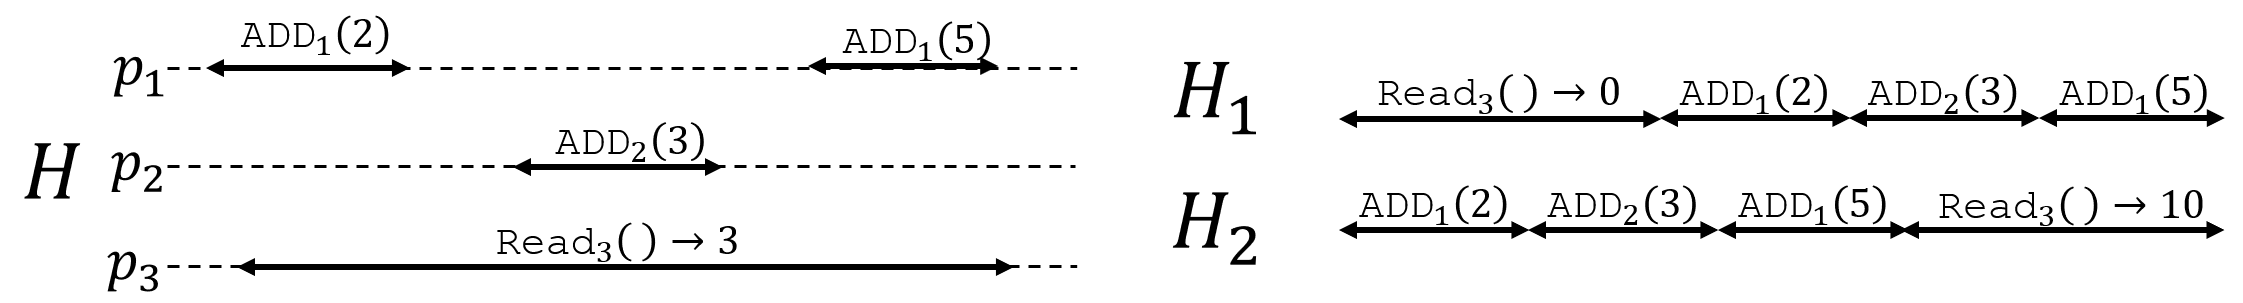
\includegraphics[width=0.7\textwidth]{graphics/ivl/adderIVL.png}
    \caption{A possible concurrent history of the IVL batched counter: $p_1$ and
    $p_2$ update their local registers, while $p_3$ reads. $p_3$ returns an intermediate
    value between the counter's state when it starts, which is $0$, and the counter's state when it completes, which is $10$.
    In $H_1$, the {\sc read} operation before all concurrent {\sc update} operations,
    and in $H_2$ it is ordered after all concurrent ones. Its return value is bounded between
    those in $H_1$, where it returns $0$, and $H_2$, where it returns $10$.}
    \label{ivl-img:adderIVL}
\end{figure}

Algorithm~\ref{ivl-alg:ivl-adder} presents an IVL implementation of a batched counter
with $n$ processes using an array $v$ of $n$ SWMR registers.
The implementation is a trivial parallelization: an {\sc update} operation increments
the process's local
register while a {\sc read} scans all registers and returns their sum. This
implementation is not linearizable because the reader does not take an atomic snapshot
of $v[1 \dots n]$. Thus, it may see a later {\sc update}
and miss an earlier one, as illustrated in Figure~\ref{ivl-img:adderIVL}.
\inred{First, note that the following observation follows from
the pseudo-code of Algorithm~\ref{ivl-alg:ivl-adder}:}
We now prove the following lemma:
\begin{lemma}
    Algorithm~\ref{ivl-alg:ivl-adder} is an IVL implementation of a batched counter.
    \label{ivl-lmma:ivl-adder}
\end{lemma}
\begin{proof}
    Let $H$ be a well-formed history of a schedule $\sigma$ of Algorithm~\ref{ivl-alg:ivl-adder},
    \inred{and let $\alpha$ be its execution}.
    We first complete $H$ be adding appropriate responses to all {\sc update} operations
    that updated $v$ (executed Line~\ref{ivl-alg:ivl-adder:l:inc}), and removing all other pending {\sc update} and {\sc read} operations.
    We denote this completed history as $H'$.

    Let $H_1$ be a linearization of $H'^?$ given by ordering {\sc update} operations by their
    return steps, and ordering {\sc read} operations after all preceding operations in $H'^?$ and before concurrent {\sc update} operations.
    {\sc read} operations assigned to the same point are ordered by their invoke steps.
    Let $H_2$ be a linearization of $H'^?$ given by ordering {\sc update} operations by their
    invocations, and ordering {\sc read} operations operations after all operations that precede them in $H'^?$ and after concurrent {\sc update} operations. 
    {\sc read} operations assigned to the same point are ordered by their invoke steps.
    Let $\alpha_i$ for $i=1,2$ be a sequential execution of a batched counter with history $\tau_\mathcal{H}(H_i)$.

    By construction, $H_1$ and $H_2$ are linearizations of $H'^?$ (as they adhere to real-time order).
    Let $R$ be some {\sc read} operation that completes
    in $H$. Let $v_{\alpha}[1 \dots n]$ be the array as read by $R$ in $\alpha$, $v_{\alpha_1}[1 \dots n]$ as read by $R$ in $\alpha_1$
    and $v_{\alpha_2}[1 \dots n]$ as read by $R$ in $\alpha_2$. To show that
    $\text{ret}(R, \tau_\mathcal{H}(H_1)) \leq \text{ret}(R, H) \leq \text{ret}(R, \tau_\mathcal{H}(H_2))$,
    we show that $v_1[j] \leq v[j] \leq v_2[j]$ for every index $1 \leq j \leq n$.

    %For any index $j$, only $p_j$ can increment $v[j]$.
    For any index $j$, $v[j]$ is incremented with non-negative values. By the construction of $H_1$, all {\sc update}
    operations that update $v[j]$ that precede $R$ in $H$ also precede it in $H_1$. Therefore, $v_{\alpha_1}[j] \leq v_{\alpha}[j]$.
    By the construction of $H_2$, all {\sc update} operations that update $v[j]$ that precede $R$ in $H$ also precede it in $H_2$.
    Furthermore, in $H_2$ all concurrent operations that have updated $v[j]$ also precede $R$. As \inred{these are} all concurrent
    {\sc update} operations that update $v[j]$, $v_{\alpha}[j] \leq v_{\alpha_2}[j]$.
    % By the construction of $H_1$, all {\sc update} operations
    % that precede $R$ in $H$ also precede it in $H_1$. Therefore $v_1[j] \leq v[j]$. Assume by contradiction that $v[j] > v_2[j]$.
    % Consider all concurrent {\sc update} operations to $R$. After all concurrent {\sc update} operations end, the value
    % of index $j$ is $v' \geq v[j] > v_2[j]$. However, by construction, $R$ is ordered after all concurrent {\sc update}
    % operations in $H_2$, therefore $v' \leq v_2[j]$. This is a contradiction, and therefore $v[j] \leq v_2[j]$.

    As all entries in the array are non-negative, it follows that $\sum_{j=1}^n v_{\alpha_1}[j] \leq \sum_{j=1}^n v_{\alpha}[j] \leq \sum_{j=1}^n v_{\alpha_2}[j]$, and
    therefore $\text{ret}(R, \tau_\mathcal{H}(H_1)) \leq \text{ret}(R, H) \leq \text{ret}(R, \tau_\mathcal{H}(H_2))$.
\end{proof}

This algorithm can efficiently implement a distributed or NUMA-friendly counter, as processes
only access their local registers \inred{for updaing values} thereby lowering the cost of incrementing the counter.\inred{Such
an implementation is highly efficient when update operations are much more frequent than read operations.}
This is of great importance, as memory latencies are often the main bottleneck in shared object emulations~\cite{mahapatra1999processor}.
As there are no waits in
either {\sc update} or {\sc read}, it follows that the algorithm is wait-free. Furthermore, the {\sc read} step complexity
is $O(n)$, and the {\sc update} step complexity is $O(1)$. Thus, we have shown the following theorem:
\begin{theorem}
    There exists a bounded wait-free IVL implementation of a batched counter using only SWMR registers, such that the step complexity of {\sc update} is $O(1)$
    and the step complexity of {\sc read} is $O(n)$.
\end{theorem}

% \subsubsection{Lower bound for linearizable batched counter object}
% \label{ivl-ssec:lower-bound}

% The incentive for using an IVL batched counter instead of a linearizable one stems
% from a lower bound on the step-complexity of a wait-free linearizable batched counter implementation from SWMR registers.
% To show the lower bound we first define the binary snapshot object.
% A \emph{snapshot object} has $n$ components written by separate processes, and allows a reader to
% capture the shared variable states of all $n$ processes instantaneously. We
% consider the \emph{binary snapshot object}, in which each state component may be either $0$ or $1$~\cite{hoepman1993binary}. The object
% supports the {\sc update}$_i$($v$) and {\sc scan} operations, where the former sets the state of component $i$
% to value a $v \in \{0,1\}$ and the latter returns all processes states instantaneously.
% It is trivial that the {\sc scan} operation must read all states, therefore its lower bound step complexity
% is $\Omega(n)$. Israeli and Shriazi~\cite{israeli1998time} show that the {\sc update} step complexity
% of any implementation of a snapshot object from SWMR registers is also $\Omega(n)$. This lower bound
% was shown to hold also for multi writer registers~\cite{attiya2006complexity}. While
% their proof was originally given for a multi value snapshot object, it holds in the binary case as well~\cite{hoepman1993binary}.

% \begin{algorithm}
%     \begin{algorithmic}[1]
%         % \begin{multicols}{2}

%         \State local variable $v_i$ \Comment{Initialized to $0$}
%         \State shared batched counter object $\mathit{BC}$
%         \Statex
%         \Procedure{update$_i$}{$v$}
%         \State \algorithmicif\ $v_i = v$\ \algorithmicthen\ \textbf{return} \label{ivl-l:skip}
%         \State $v_i \gets v$
%         \State \algorithmicif\ $v = 1$\ \algorithmicthen\ $\mathit{BC}$.{\sc update}$_i$($2^i$) \label{ivl-l:set-1}
%         \State \algorithmicif\ $v = 0$\ \algorithmicthen\ $\mathit{BC}$.{\sc update}$_i$($2^n - 2^i$) \label{ivl-l:set-0}
%         \EndProcedure
%         % \columnbreak
%         \Procedure{scan}{}
%         \State $\mathit{sum} \gets \mathit{BC}$.{\sc read}() \label{ivl-l:read} % $\mod 2^n$
%         \State $v[0 \dots n-1] \gets [0 \dots 0]$ \Comment{Initialize an array of $0$'s}
%         \For{$i : 0 \leq i \leq n-1$}
%         \State \algorithmicif\ bit $i$ is set in $\mathit{sum}$\ \algorithmicthen\ $v[i] \gets 1$ \label{ivl-l:check-set}
%         \EndFor
%         \State \textbf{return} $v[0 \dots n-1]$
%         \EndProcedure
%     % \end{multicols}
%     \end{algorithmic}
%     \caption{Algorithm for process $p_i$, solving binary snapshot with a batched counter object.}
%     \label{ivl-alg:bs-with-adder}
% \end{algorithm}

% To show a lower bound on the {\sc update} operation of wait-free linearizable batched counters,
% we show a reduction from a binary snapshot to a batched counter in
% Algorithm~\ref{ivl-alg:bs-with-adder}. It uses a local variable $v_i$ and a shared batched counter object.
% In a nutshell, the idea is to encode the value of the $i^\text{th}$ component
% of the binary snapshot using the $i^\text{th}$ least significant bit of the counter.
% When the component changes from $0$ to $1$, {\sc update}$_i$ adds $2^i$, and when it changes from $1$ to $0$,
% {\sc update}$_i$ adds $2^n - 2^i$. We now prove the following invariant:
% \begin{invariant}
%     At any point $t$ in history $H$ of a sequential execution of Algorithm~\ref{ivl-alg:bs-with-adder},
%     the sum held by the counter is $c \cdot 2^n + \sum_{i=0}^{n-1}v_i2^i$,
%     such that $v_i$ is the parameter passed to the last invocation of {\sc update}$_i$ in $H'$ before $t$ if such invocation
%     exists, and $0$ otherwise, for some integer $c \in \mathbb{N}$.
%     \label{ivl-inv:sum}
% \end{invariant}
% \begin{proof}
%     We prove the invariant by induction on the length of $H$, i.e., the number of invocations in $H$,
%     denoted $t$. As $H$ is a sequential history, each invocation is followed by a response.
%     %\par{\textbf{Base:}}
%     The base if for $t=0$, i.e., $H$ is the empty execution. In this case no updates
%     have been invoked, therefore $v_i=0$ for all $0 \leq i \leq n-1$. The sum returned by the counter
%     is $0$. Choosing $c=0$ satisfies the invariant.
%     %\par{\textbf{Induction step:}}
%     Our induction hypothesis is that the invariant holds for a history of length $t$.
%     We prove that it holds for a history of length $t+1$. The last invocation can be either a {\sc scan}, or an {\sc update}($v$)
%     by some process $p_i$. If it is a {\sc scan}, then the counter value doesn't change and the invariant
%     holds. Otherwise, it is an {\sc update}($v$). Here, we note two cases. Let $v_i$ be $p_i$'s value
%     prior to the {\sc update}($v$) invocation. If $v = v_i$, then the {\sc update} returns without altering the sum
%     and the invariant holds. Otherwise, $v \neq v_i$. We analyze two cases, $v=1$ and $v=0$. If $v=1$, then $v_i=0$.
%     The sum after the update is $c \cdot 2^n + \sum_{i=0}^{n-1}v_i2^i + 2^i=c \cdot 2^n + \sum_{i=0}^{n-1}v_i'2^i$, where
%     $v_j'=v_j$ if $j \neq i$, and $v'_i = 1$, and the invariant holds. If $v=0$, then $v_i=1$.
%     The sum after the update is $c \cdot 2^n + \sum_{i=0}^{n-1}v_i2^i + 2^n - 2^i = (c+1) \cdot 2^n + \sum_{i=0}^{n-1}v_i'2^i$,
%     where $v_j'=v_j$ if $j \neq i$, and $v'_i = 1$, and the invariant holds.
% \end{proof}

% Using the invariant, we prove the following lemma:
% \begin{lemma}
%     For any sequential history $H$, if a {\sc scan} returns $v_i$, and {\sc update}$_i$($v$) is the last update invocation in $H$
%     prior to the {\sc scan}, then $v_i = v$. If no such update exists, then $v_i=0$.
%     \label{ivl-lmma:scan-correctness}
% \end{lemma}
% \begin{proof}
%     Let $S$ be a {\sc scan} in $H'$. Consider the sum $\textit{sum}$ as read by scan $S$.
%     From Invariant~\ref{ivl-inv:sum}, the value held by the counter is $c \cdot 2^n + \sum_{i=0}^{n-1}v_i2^i$.
%     There are two cases, either there is an update invocation prior to $S$, or there isn't. If there isn't, then by
%     Invariant~\ref{ivl-inv:sum} the corresponding $v_i=0$. The process sees bit $i=0$,
%     and will return $0$. Therefore, the lemma holds.

%     Otherwise, there is a an update prior to $S$ in $H$. As the sum is equal to $c \cdot 2^n + \sum_{i=0}^{n-1}v_i2^i$,
%     by Invariant~\ref{ivl-inv:sum}, bit $i$ is equal to $1$ iff the parameter passed to the last invocation of update was $1$.
%     Therefore, the scan returns the parameter of the last update and the lemma holds.
% \end{proof}

% \begin{lemma}
%     Algorithm~\ref{ivl-alg:bs-with-adder} implements a linearizable binary snapshot using a linearizable batched counter.
%     \label{ivl-lmma:reduction}
% \end{lemma}
% \begin{proof}
%     Let $H$ be a history of Algorithm~\ref{ivl-alg:bs-with-adder}, and let $H'$
%     be $H$ where each operation is linearized at its access to the linearizable batched counter, or
%     its response if $v_i = v$ on line~\ref{ivl-l:skip}.
%     Applying Lemma~\ref{ivl-lmma:scan-correctness} to $H'$, we get $H' \in \mathcal{H}$ and therefore $H$ is linearizable.
% \end{proof}

% It follows from the algorithm that if the counter
% object is bounded wait-free then the {\sc scan} and {\sc update} operations are bounded wait-free. Therefore, the lower
% bound proved by Israeli and Shriazi~\cite{israeli1998time} holds, and the {\sc update} must take $\Omega(n)$
% steps. Other than the access to the counter in the {\sc update} operation, it takes
% $O(1)$ steps. Therefore, the access to the counter object must take $\Omega(n)$ steps. We have proven the following theorem.
% \begin{theorem}
%     For any linearizable wait-free implementation of a batched counter object with $n$ processes from SWMR registers, the step-complexity
%     of the {\sc update} operation is $\Omega(n)$.
%     \label{ivl-thm:lower-bound}
% \end{theorem}


\subsection{Relaxed shared CountMin sketch}
\label{ivl-ssec:countMin}

In this Section we present a relaxed CountMin sketch. Section~\ref{ivl-sssec:cm} presents a concurrent
IVL implementation, and shows that this implementation isn't linearizable.
Section~\ref{ivl-sssec:relaxed-cm} presents the $r$-relaxed IVL CM sketch.

\subsubsection{IVL CountMin sketch}
\label{ivl-sssec:cm}

Cormode et al. propose the \emph{CountMin (CM)} sketch~\cite{CountMin}, which
estimates the frequency of an item $a$, denoted $f_a$, in a data stream, where the data stream
is over some alphabet $\Sigma$. The CM sketch supports two operations: {\sc update}($a$),
which updates the object based on $a \in \Sigma$, and {\sc query}($a$), which returns
an estimate on the number of {\sc update}($a$) calls that preceded the query. \inred{The number
of {\sc update} operations that precede a query is called the \emph{stream length},
generally denoted by $N$.}

The sequential algorithm's underlying data structure is a matrix $c$ of $w \times d$ counters,
for some parameters $w,d$ determined according to the desired error and probability bounds.
The sketch uses $d$ hash functions $h_i: \Sigma \mapsto [1,w]$, for $1 \leq i \leq d$.
The hash functions are generated using the random coin flip vector $\vv{c}$,
and have certain mathematical properties whose details are not essential for understanding this paper.
The algorithm's input (i.e., the schedule) is generated by a so-called \emph{weak adversary}, namely,
the input is independent of the randomly drawn hash functions.
% These hash functions are drawn randomly by a
% \emph{weak adversary}, i.e., the schedule is independent from the hash functions.

The CountMin sketch, denoted $CM(\vv{c})$, is illustrated in Figure~\ref{ivl-img:cmSketch}, and its
pseudo-code is given in Algorithm~\ref{ivl-alg:count-min}.
On {\sc update}($a$), the sketch increments counters $c[i][h_i(a)]$ for every
$1 \leq i \leq d$. {\sc query}($a$) returns $\hat{f}_a=\min_{1 \leq i \leq d}\{c[i][h_i(a)]\}$.

\begin{algorithm}
    \begin{algorithmic}[1]
        % \begin{multicols}{2}

        \State array $c[1 \dots d][1 \dots w]$ \Comment{Initialized to $0$}
        \State hash functions $h_1, \dots h_d$ \Comment{$h_i: \Sigma \mapsto [1,w]$, initialized using $\vv{c}$}
        \Statex
        \Procedure{update}{$a$}
        \For{$i : 1 \leq i \leq d$}
        \State atomically increment $c[i][h_i(a)]$ \label{ivl-l:counter-inc}
        \EndFor
        \EndProcedure

        % \columnbreak

        \Procedure{query}{$a$}
        \State $min \gets \infty$
        \For{$i : 1 \leq i \leq d$}
        \State $c \gets c[i][h_i(a)]$ \label{ivl-l:read-min}
        \State \algorithmicif\ $min > c$ \ \algorithmicthen\ $min \gets c$ \label{ivl-l:min-update}
        \EndFor
        \State \textbf{return} $min$
        \EndProcedure
    % \end{multicols}
    \end{algorithmic}
    \caption{CountMin($\vec{c}$) sketch.}
    %\caption{CountMin($\vv{c}$) sketch.}
    \label{ivl-alg:count-min}
\end{algorithm}

Cormode et al. show that, for desired bounds $\delta$ and $\alpha$, given appropriate values of $w$ and $d$, with probability
at least $1-\delta$, the estimate of a query returning $\hat{f}_a$ is bounded by $f_a \leq \hat{f}_a \leq f_a + \alpha N$,
where \inred{$N$ is the number of elements in the stream} and $f_a$ is the ideal value.
Thus, for $\epsilon= \alpha N$, CM is a sequential $(\epsilon, \delta)$-bounded
object. Its sequential specification distribution is $\{CM(\vv{c})\}_{\vv{c} \in \Omega^\infty}$.

% \afterpage{
  \begin{figure}
    \begin{center}
     \includegraphics[width=0.4\textwidth,trim=10 0 30 10,clip]{graphics/ivl/cmSketch.png}
      \caption[The LOF caption]{An example CountMin sketch, of size $w \times d$, where $h_1(a)=6$, $h_2(a)=4$ and $h_d(a)=w$.\footnotemark}
     \label{ivl-img:cmSketch}
    \end{center}
  \end{figure}
  \footnotetext{Source: \url{https://stackoverflow.com/questions/6811351/explaining-the-count-sketch-algorithm}, with alterations.}
% }
% \begin{figure}[b]
%     \centering
%     \includegraphics[width=0.3\textwidth,trim=10 0 30 10,clip]{images/cmSketch.png}
%     %\caption{An example CountMin sketch, of size $w \times d$, where $h_1(a)=6$, $h_2(a)=4$ and $h_d(a)=w$.\footnote{Image from https://stackoverflow.com/questions/6811351/explaining-the-count-sketch-algorithm}}
%     \caption[Caption for LOF]{An example CountMin sketch, of size $w \times d$, where $h_1(a)=6$, $h_2(a)=4$ and $h_d(a)=w$.\protect\footnote{Image from https://stackoverflow.com/questions/6811351/explaining-the-count-sketch-algorithm}}
%     \label{ivl-img:cmSketch}
% \end{figure}

Proving an error bound for an efficient parallel implementation of the CM sketch is not trivial.
Any linearizable implementation, and even an $r$-relaxed linearizable, such as that of
Rinberg et al.~\cite{rinberg2019fast}, requires the query to take an
atomic snapshot of the matrix~\cite{ovens2019strongly}, which we forgo in Algorithm~\ref{ivl-alg:count-min}.
Distributional linearizability~\cite{alistarh2018distributionally} necessitates an analysis of the error bounds
directly in the concurrent setting, without leveraging the sketch's existing analysis for the sequential setting.

Instead, we utilize IVL to leverage the sequential analysis for a parallelization that
is not strongly linearizable (or indeed linearizable), without using a
snapshot. Consider the straightforward parallelization of the CM sketch,
whereby the operations of Algorithm~\ref{ivl-alg:count-min} may be invoked concurrently
and each counter is atomically incremented \inred{(e.g., using a FAA atomic operation~\cite{atomic-inc})} on
line~\ref{ivl-l:counter-inc} and read on line~\ref{ivl-l:read-min}. We call
this parallelization $PCM$. We next prove that it is IVL.% Its error analysis then follows from Theorem~\ref{ivl-thm:SIVL-bound}.


\begin{lemma}
    %The straightforward parallelization of the CM sketch Algorithm~\ref{ivl-alg:count-min} is IVL.
    $PCM$ is an IVL implementation of $CM$.
    \label{ivl-lmma:count-min-ivl}
\end{lemma}
\begin{proof}
    Let $H$ be a history of an execution $\sigma$ of $PCM$.
    Let $H_1$ be a linearization of $H^?$ such that every query is linearized prior to every
    concurrent update, and let $H_2$ be a linearization of $H^?$ such that every query is linearized after every
    concurrent update. Let $\sigma_i$ for $i=1,2$ be a sequential execution of $CM$ with history $H_i$.
    Consider some $Q=${\sc query}($a$) that returns in $H$, and let $U_1,\dots,U_k$ be the concurrent updates to $Q$.
    
    Denote by $c_\sigma(Q)[i]$ the value read by $Q$ from $c[i][h_i(a)]$ in line~\ref{ivl-l:read-min} of Algorithm~\ref{ivl-alg:count-min}
    in an execution $\sigma$.
    % Let $c_a = \left\{c[1][h_1(a)], \dots, c[d][h_d(a)]\right\}$ be the vector of counters associated with $a$ as seen by $Q$ in $H$.
    % In a similar fashion Let $c_a^i= \left\{c^i[1][h_1(a)], \dots, c^i[d][h_d(a)]\right\}$ be the vector
    % as seen by $Q$ in $H_i$.
    As processes only increment counters, for every $1 \leq i \leq d$, $c_{\sigma}(Q)[i]$ is at least
    $c_{\sigma_1}(Q)[i]$ (the value when the query starts) and at most $c_{\sigma_2}(Q)[i]$ (the value when
    all updates concurrent to the query complete). Therefore,
    $c_{\sigma_1}(Q)[i] \leq c_{\sigma}(Q)[i] \leq c_{\sigma_2}(Q)[i]$.

    Consider a randomly sampled coin flip vector $\vv{c} \in \Omega^\infty$.
    Let $j$ be the loop index the last time query $Q$ alters the value of its local variable $min$ (line~\ref{ivl-l:min-update}),
    i.e., the index of the minimum read value.
    As a query in a history of $CM(\vv{c})$ returns the minimum value in the array, $\text{ret}(Q, \tau_{CM(\vv{c})}(H_1)) \leq c_{\sigma_1}(Q)[j]$. Furthermore, $\text{ret}(Q, \tau_{CM(\vv{c})}(H_2))$
    is at least $c_{\sigma}(Q)[j]$, otherwise $Q$ would have read this value and returned it instead. Therefore:
    \[
        \text{ret}(Q, \tau_{CM(\vv{c}))}(H_1)) \leq \text{ret}(Q, H(PCM, \sigma, \vv{c})) \leq \text{ret}(Q, \tau_{CM(\vv{c})}(H_2))
    \]
    As needed.
\end{proof}

Combining Lemma~\ref{ivl-lmma:count-min-ivl} and Theorem~\ref{ivl-thm:SIVL-bound}, and by utilizing the sequential
error analysis from~\cite{CountMin}, we have shown the following corollary:
\begin{corollary}
    Consider a concurrent history $H$ of PCM with parameters $(\epsilon, \delta)$, with a stream of length $N$.
    Let $\hat{f}_a$ be a return value from query $Q$ with parameter $a$ in $H$. Let $f_a^\text{start}$ be the ideal frequency of element $a$
    \inred{at the invocation of $Q$}, and let $f_a^\text{end}$ be the ideal frequency of element $a$ \inred{at the response of $Q$}. Then:
    \[ f_a^\text{start} \leq \hat{f}_a \leq f_a^\text{end} + \epsilon \text{ with probability at least } 1-\delta.\]
\end{corollary}
\inred{
\begin{proof}
    Let $CM$ be a sequential $(\epsilon, \delta)$-bounded object. Lemma~\ref{ivl-lmma:count-min-ivl} proves that $PCM$
    is an IVL implementation of $CM$, therefore, by Theorem~\ref{ivl-thm:SIVL-bound}, PCM implements a concurrent
    $(\epsilon, \delta)$-bounded object.

    Consider some concurrent history $H$ containing $N$ update operations, and consider some query $Q$ of element $a$
    that returns in $H$. Let $H^{\text{start}}$ be the prefix of $H$ up to the invocation of $Q$, where all pending operations
    are removed. Let $f_a^\text{start}$ be the number of update operations in $H^{\text{start}}$ with parameter $a$. As each
    update operation increments the counters $Q$ reads, and they all precede $Q$, then $f_a^\text{start} \leq v^{\mathcal{I}}_{min}(H,Q)$.
    
    Let $H^{\text{end}}$ be the prefix of $H$ up to the response of $Q$, where all pending operations
    are completed.Let $f_a^\text{end}$ be the number of update operations in $H^{\text{end}}$ with parameter $a$. As each
    update operation increments the counters $Q$ reads, then $f_a^\text{end} \geq v^{\mathcal{I}}_{min}(H,Q)$.
    Therefore:
    \[ f_a^\text{start} - \epsilon \leq \hat{f}_a \leq f_a^\text{end} + \epsilon \text{ with probability at least } 1-\delta.\]

    This can be further improved by noting that the $Q$ returns at least $f_a^\text{start}$, as it cannot read the counters
    with values less than $f_a^\text{start}$. Therefore:
    \[ f_a^\text{start} \leq \hat{f}_a \leq f_a^\text{end} + \epsilon \text{ with probability at least } 1-\delta.\]
\end{proof}
}

The following example demonstrates that $PCM$ is not a linearizable implementation of $CM$.

\begin{example}
    Consider the following execution $\sigma$ of $PCM$: Assume that $\vv{c}$ is such that $h_1(a)=h_2(a)=1$, $h_1(b)=2$ and $h_2(b)=1$.
    Assume that initially
    \[ c=\CM{1}{4}{2}{3}. \]
    First, process $p$ invokes $U=${\sc update}$(a)$ which increments $c[1][1]$ to $2$ and stalls.
    Then, process $q$ invokes $Q_1=${\sc query}$(a)$ which reads $c[1][1]$ and $c[2][1]$ and returns $2$,
    followed by $Q_2=${\sc query}$(b)$ which reads $c[1][2]$ and $c[2][1]$ and returns $2$. Finally, process $p$ increments $c[2][1]$ to be $3$.

    Assume by contradiction that $H$ is a linearization of $\sigma$, and $H \in CM(\vv{c})$.
    The return values imply that $U \prec_H Q_1$ and $Q_2 \prec_H U$. As $H$ is a linearization, it maintains
    the partial order of operations in $\sigma$, therefore $Q_1 \prec_H Q_2$. A contradiction.
    % Consider a CM sketch of size $2 \times 2$, such that $h_1(a)=h_2(a)=1$ and $h_1(b)=2, h_2(b)=1$ for
    % two elements $a,b \in \Sigma$. Consider a \CM{1}{4}{2}{3}, and consider process $p$
    % which executes $Q_1=${\sc query}$(a)$ followed by $Q_1=${\sc query}$(b)$, and process
    % $q$ which executes {\sc update}$(a)$ concurrently to the queries. Let $H$ be the arising
    % history, and let $f$ be the mapping under linearizability. Query $Q_1$ may read
    % \CM{2}{4}{2}{3} thereby returning $2$, implying $U \prec_{f(H)} Q_1$.
    % $Q_2$ may read the same state thereby returning $2$, implying $Q_2 \prec_{f(H)} U$.
    % However, $Q_1 \prec_{f(H)} Q_2$ due to process order.
\end{example}


% \begin{example}
%     Consider a CM sketch of size $2 \times 2$, such that $h_1(a)=h_2(a)=1$ and $h_1(b)=2, h_2(b)=1$ for
%     two elements $a,b \in \Sigma$. Consider a \CM{1}{4}{2}{3}, and consider process $p$
%     which executes $Q_1=${\sc query}$(a)$ followed by $Q_1=${\sc query}$(b)$, and process
%     $q$ which executes {\sc update}$(a)$ concurrently to the queries. Let $H$ be the arising
%     history, and let $f$ be the mapping under linearizability. Query $Q_1$ may read
%     \CM{2}{4}{2}{3} thereby returning $2$, implying $U \prec_{f(H)} Q_1$.
%     $Q_2$ may read the same state thereby returning $2$, implying $Q_2 \prec_{f(H)} U$.
%     However, $Q_1 \prec_{f(H)} Q_2$ due to process order.
% \end{example}

% From Theorem~\ref{ivl-thm:SIVL-bound} we have parallelized the CM sketch while
% preserving bounds. The next step is to calculate these bounds. Note that
% the CountMin sketch is an $(\epsilon n, \delta)$-bounded object. Therefore,
% from Theorem~\ref{ivl-thm:SIVL-bound}, the concurrent implementation is also
% $(\epsilon n, \delta)$-bounded. More accurately, Cormode et al. show that if $f_a$ is the true count of $a$, and
% the stream length is $n$, then the approximation $\hat{f}_a$
% is in the range $f_a \leq \hat{f}_a \leq f_a + \epsilon n$, with
% probability at least $1-\delta$. In fact, the left inequality is true with
% probability $1$, it is only the right hand inequality which is bound with probability.
% Consider $k$ concurrent
% writes to some query $Q$ of count $a$, of which $l \leq k$ are {\sc update} operations
% which parameter $a$ (i.e., if the true value before is $f_a$,
% then true value after is $f_a + l$), then the returned value is in the
% range $f_a \leq \hat{f}_a \leq f_a + l + \epsilon(n + k)$
% with probability at least $1-\delta$.

\subsubsection{Relaxed IVL CM sketch}
\label{ivl-sssec:relaxed-cm}

Using the $r$-relaxed IVL form, we can create a buffered CM sketch
by using a similar framework to Rinberg et al.~\cite{rinberg2019fast}. The
\textsc{update} operations are buffered locally by updating threads until a certain threshold
is reached. The resulting matrix is then merged into the shared CM sketch,
which is updated element by element. 

This buffered approach allows for far better memory locality. Rather than every
\textsc{update} operating on shared memory, most operations are local. This
leads to better cache utilization, and forgoes expensive NUMA memory accesses.

In Rinberg et al., a \textsc{query} takes a strongly linearizable snapshot of the
current global state, and applies the query
to it.  In a CM sketch, a linearizable snapshot is an expensive operation -- it requires
an atomic snapshot. Using an IVL query
forgoes the need for a strongly linearizable snapshot, while retaining error bounds.

The buffered IVL CM sketch is $r$-relaxed IVL with respect to $\mathcal{H}_{CM}$, where
$r=2Wb$, where $W$ is the number of worker threads and $b$ is the local buffer size (i.e.,
the number of updates processed between propagations).

The error analysis follows from the relaxation and the definition of IVL. Consider some query $Q$ on $a$
that returns $v$, and let $S^{start}$ and $S^{end}$ be the state of the system at the start and end of
$Q$'s execution, respectively.
%Let $N$ be the length of the stream and $v^{start}$ be the number of times $a$ appears in the stream before $S^{start}$.
\inred{Let $v^{start}$ be the number of times $a$ appears in the stream before $S^{start}$, let
$v^{end}$ be the number of times $a$ appears in the stream before $S^{end}$, and let $N^{end}$
be the length of the stream at $S^{end}$.}
\[ v^{start} - r \leq v \leq  v^{end} + \epsilon N^{end}. \]

\subsection{Non-atomic iterators}
\label{ivl-ssec:sets-and-iterators}

While until now we focused on numerical objects, the idea behind IVL can be
expanded to include other types of objects as well. For example, iterators
in map and set data structures (like skiplists and search trees) typically return a
non-atomic scan of the set of keys -- or items -- in the data structure~\cite{arbel2018harnessing, meir2020oak}.
We show that the semantics of such scan operations are naturally captured using IVL.
Consider a data structure supporting three operations, (1) \textsc{insert}, (2) \textsc{delete},
and (3) \textsc{scan}.
The sequential specification $\mathcal{H}_{MAP}$ is straightforward, a \textsc{scan}
returns all elements that were inserted before it and were not deleted before it.

The concurrent semantics are typically defined as follows~\cite{arbel2018harnessing, meir2020oak}:
\begin{definition}[Non-atomic \textsc{Scan} operation semantics]
Consider a scan operation, returning some set $S$. Let $K$ be the elements that have
been inserted prior to the scan's invocation and have not been deleted before the scan. Let
$I$ be the elements being inserted concurrently to the scan, and let $D$ be the set of elements
that are removed concurrently to the scan. Then $K \setminus D \subseteq S \subseteq K \cup I$.
\label{ivl-def:scan}
\end{definition}

This definition resembles IVL with the partial order of set containment. However, IVL also
adheres to program order. So if a thread adds element $a$, then removes it, then 
adds element $b$, an IVL scan result cannot contain both $a$ and $b$, which is allowed
by Definition~\ref{ivl-def:scan}.

We can, nevertheless, use IVL to capture the correctness semantics of such non-atomic
iterators as specified by Definition~\ref{ivl-def:scan}.
To this end, we add an auxiliary history variable both at the concrete level
(the data structure is augmented to track its removals in an auxiliary history variable holding
tombstones) and at the abstract level (the \textsc{scan} in the augmented sequential
specification returns a set including tombstones).
The algorithm augmented
with the auxiliary variable is an IVL implementation of the augmented sequential specification.  
The \textsc{insert}($a$) operation inserts $a$ into the auxiliary variable.
The \textsc{delete}($a$) operation inserts a tombstone for $a$, denoted $-a$, into the auxiliary variable. The
concrete return value is defined via a function $f$ that returns the
set of elements that are included and do not have tombstones in the
auxiliary variable, e.g., $f(\{a,-a,b\}) = \{b\}$.

Formally, let $\mathcal{V}$ be the set of all possible elements, and denote the possible
tombstones as $\mathcal{V}^-=\{-v| v \in \mathcal{V}\}$. The auxiliary variable
is some $S \in 2^{\mathcal{V} \cup \mathcal{V}^-}$. We define $f : 2^{\mathcal{V} \cup \mathcal{V}^-} \mapsto 2^{\mathcal{V}}$  as:
$f(S) = \{v| v \in S \wedge -v \notin S\}$.

Given the sequential specification $\mathcal{H}_{MAP}$ defined above, denote $\mathcal{H}_{T-MAP}$ as
the augmented object. The sequential specification of a \textsc{scan} operation is
also straightforward: a \textsc{scan} returns a set in $2^{\mathcal{V} \cup \mathcal{V}^-}$
consisting of all elements that were
inserted before it, and tombstones for all elements deleted before it.

We prove that IVL semantics with the auxiliary variable is equivalent to Definition~\ref{ivl-def:scan}:
\begin{lemma}   
Consider a history $H$ of a concurrent object implementing $\mathcal{H}_{MAP}$ and \inred{some} scan of it returning a set
of items $S \in 2^{\mathcal{V}}$. Denote by $\mathcal{H}_{T-MAP}$ the object augmented with
the auxiliary history variable tracking tombstones.
\inred{Then $\exists S' \in 2^{\mathcal{V} \cup \mathcal{V}^-}$ such that
returning $H$ is IVL with respect to $\mathcal{H}_{T-MAP}$ and $f(S') = S$.}
\end{lemma}
\begin{proof}
\inred{Let $H$ be a history of some concurrent object implementing $\mathcal{H}_{MAP}$},
and let $S$ be the result
of some non-atomic scan operation in $H$. Let $K$,$I$, and $D$ be as defined by
Definition~\ref{ivl-def:scan}.

$S$ satisfies Definition~\ref{ivl-def:scan}\inred{, as the object implements $\mathcal{H}_{MAP}$}. We show that $\exists S'$ such that $S'$
is IVL with respect to $\mathcal{H}_{T-MAP}$ and $f(S')=S$.

Let $H_1$ be a linearization of $H^?$ where the scan is linearized before all concurrent operations,
and let $H_2$ be a linearization of $H^?$ where the scan is linearized after all concurrent operations.
Let ${S'}_i \in 2^{\mathcal{V} \cup \mathcal{V}^-} $ be the return value of the scan in $\tau_\mathcal{H}(H_i)$,
for $i=1,2$. Let $K'$ be the set of all insertions and deletions before the scan in $H_1$,
then, by construction, $S_1' = K'$ and $S_2' = K' \cup {I \cup D^-}$. Note that $f(K')=K$.

We construct $S'$ as $S_1' \cup I' \cup D'^-$ as follows: $I' = S \cap I$, and $D' = D \setminus S$.
I.e., $I'$ is all inserted elements that are observed by $S$, and $D'$ are all deleted
elements not observed by $S$ -- meaning elements that are deleted concurrently to the scan
and not observed by it. By construction
\[ S_1' \subseteq S' = S_1' \cup I' \cup {D'}^- \subseteq S_1' \cup I \cup D^- = S_2', \]
so returning $S'$ is IVL with respect to $\mathcal{H}_{T-MAP}$.

Furthermore, by construction, $S'=K' \cup (S \cap I) \cup (D \setminus S)^-$, so
$f(S')=K \cup (S \cap I) \setminus (D \setminus S)$. By Definition~\ref{ivl-def:scan}
$K \setminus D \subseteq S \subseteq K \cup I$, we get that
$K \setminus (D \setminus S) \subseteq S \subseteq K \cup (I \cap S)$, and $f(S')=S$, as needed.
\end{proof}

\inred{We believe that instead of giving a long definition of the SCAN operation as is currently
done~\cite{arbel2018harnessing, meir2020oak}, IVL captures the semantics of such operations accurately
and succinctly.}

\subsection{Sequentially consistent IVL priority queue}
\label{ivl-ssec:priority-q}

We next show that for more complex (non-numeric) objects, IVL can be used in conjuction
with additional properties.
Consider the example of a \emph{Priority Queue (PQ)}, which supports two operations, \textsc{insert}
and \textsc{deleteMin}~\cite{van1976design, ronngren1997comparative}.
The sequential PQ holds a set of priority-element pairs.
An \textsc{insert}$(e,p)$ adds element $e$ with priority $p$ to the set,
and a \textsc{deleteMin} returns and removes the element with the lowest priority
from the set.

The set of pairs is partially ordered by priority, with ties broken
by the elements themselves.
Thus, we can use IVL to define the PQ's concurrent semantics.
However, IVL alone allows the PQ to return
elements that were never inserted, as shown in Figure~\ref{ivl-fig:PQ-IVL-not-SC}. In the example, thread $p_1$
inserts $(e_1,8)$ to the PQ and thread $p_2$ inserts $(e_2,3)$. Concurrently to the insertions, thread
$q$ removes an item from the PQ. IVL allows $q$ to return $(e_x,6)$, as $(e_2,3) \leq (e_x,6) \leq (e_2,8)$,
even though $(e_x,6)$ may be an element that was never inserted to the PQ.
Thus, an IVL PQ is meaningless. Fortunately, we can address this by requiring an additional
property along with IVL.

To disallow such spurious elements, we require that the PQ also be \emph{sequentially
consistent (SC)}~\cite{scheurich1987correct}. We note that SC and IVL are incomparable: IVL requires that sequential
executions adhere to the sequential specification, whereas SC only requires program order. For example,
Figure~\ref{ivl-fig:SC-IVL-not-IVL} shows an SC PQ that isn't IVL, and, as noted above, Figure~\ref{ivl-fig:PQ-IVL-not-SC}
shows an IVL PQ that isn't SC.

\begin{figure}[htb]
  \begin{subfigure}[b]{.45\linewidth}
      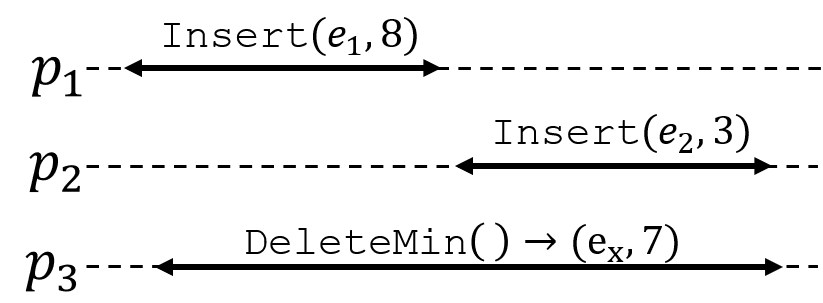
\includegraphics[width=0.32\textwidth]{graphics/ivl/PQIVLnotSC.png}
  \caption{IVL PQ that isn't SC -- $(e_x,7)$ is returned even though it was never inserted.}
  \label{ivl-fig:PQ-IVL-not-SC}
  \end{subfigure}
  \begin{subfigure}[b]{.55\linewidth}
    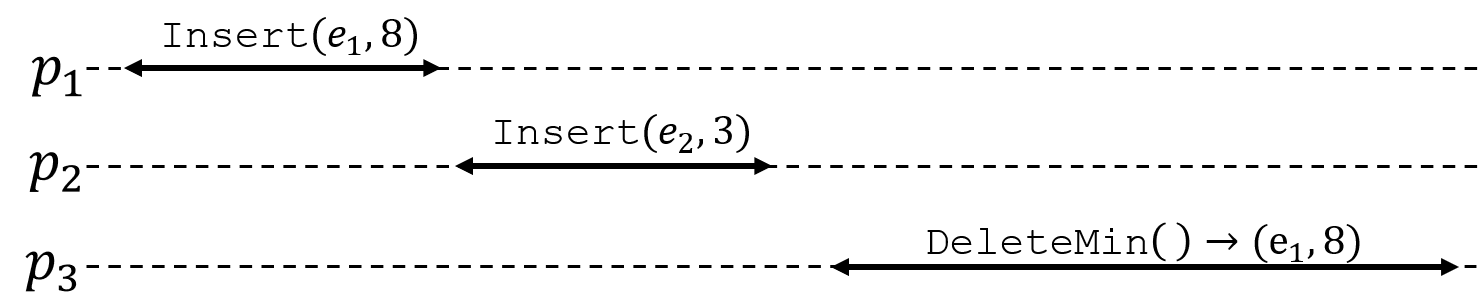
\includegraphics[width={0.58\textwidth}]{graphics/ivl/PQSCnotIVL.png}
  \caption{SC PQ that isn't IVL -- IVL adheres to real-time order, therefore $(e_2,3)$ must be returned.}
  \label{ivl-fig:SC-IVL-not-IVL}
  \end{subfigure}
  \caption{Possible histories of a priority queue under IVL only (\ref{ivl-fig:PQ-IVL-not-SC}) and SC only (\ref{ivl-fig:SC-IVL-not-IVL}).}
\end{figure}

Combining the IVL and SC properties yields a PQ that must return elements previously inserted
to the PQ and not yet deleted (by SC), yet the \textsc{deleteMin} operation may return elements
disallowed under linearizability. For example, Figure~\ref{ivl-fig:SC-IVL-and-SC} presents
a history of an IVL and SC PQ. In the
example, thread $p_1$ inserts $(e_1,8)$ to the PQ, $p_2$ then inserts $(e_2,3)$, and
then $p_1$ inserts $(e_3, 5)$. Concurrently to the insertions, $p_3$ removes an element
from the PQ. The SC property requires that the element be $(e_1,8)$, $(e_2,3)$ or $(e_3,5)$,
and the IVL property requires that the element have priority at most $8$, and at least $3$.
For example, the element $(e_3, 5)$ can be returned, which is disallowed under linearizability.

An IVL priority queue is useful when the necessary guarantee is that the popped element is one of the
top elements, but not necessarily the top one, e.g., parallel graph processing~\cite{gonzalez2012powergraph},
or belief propagation~\cite{aksenov2020scalable}.

\begin{figure}[b]
  \centering
  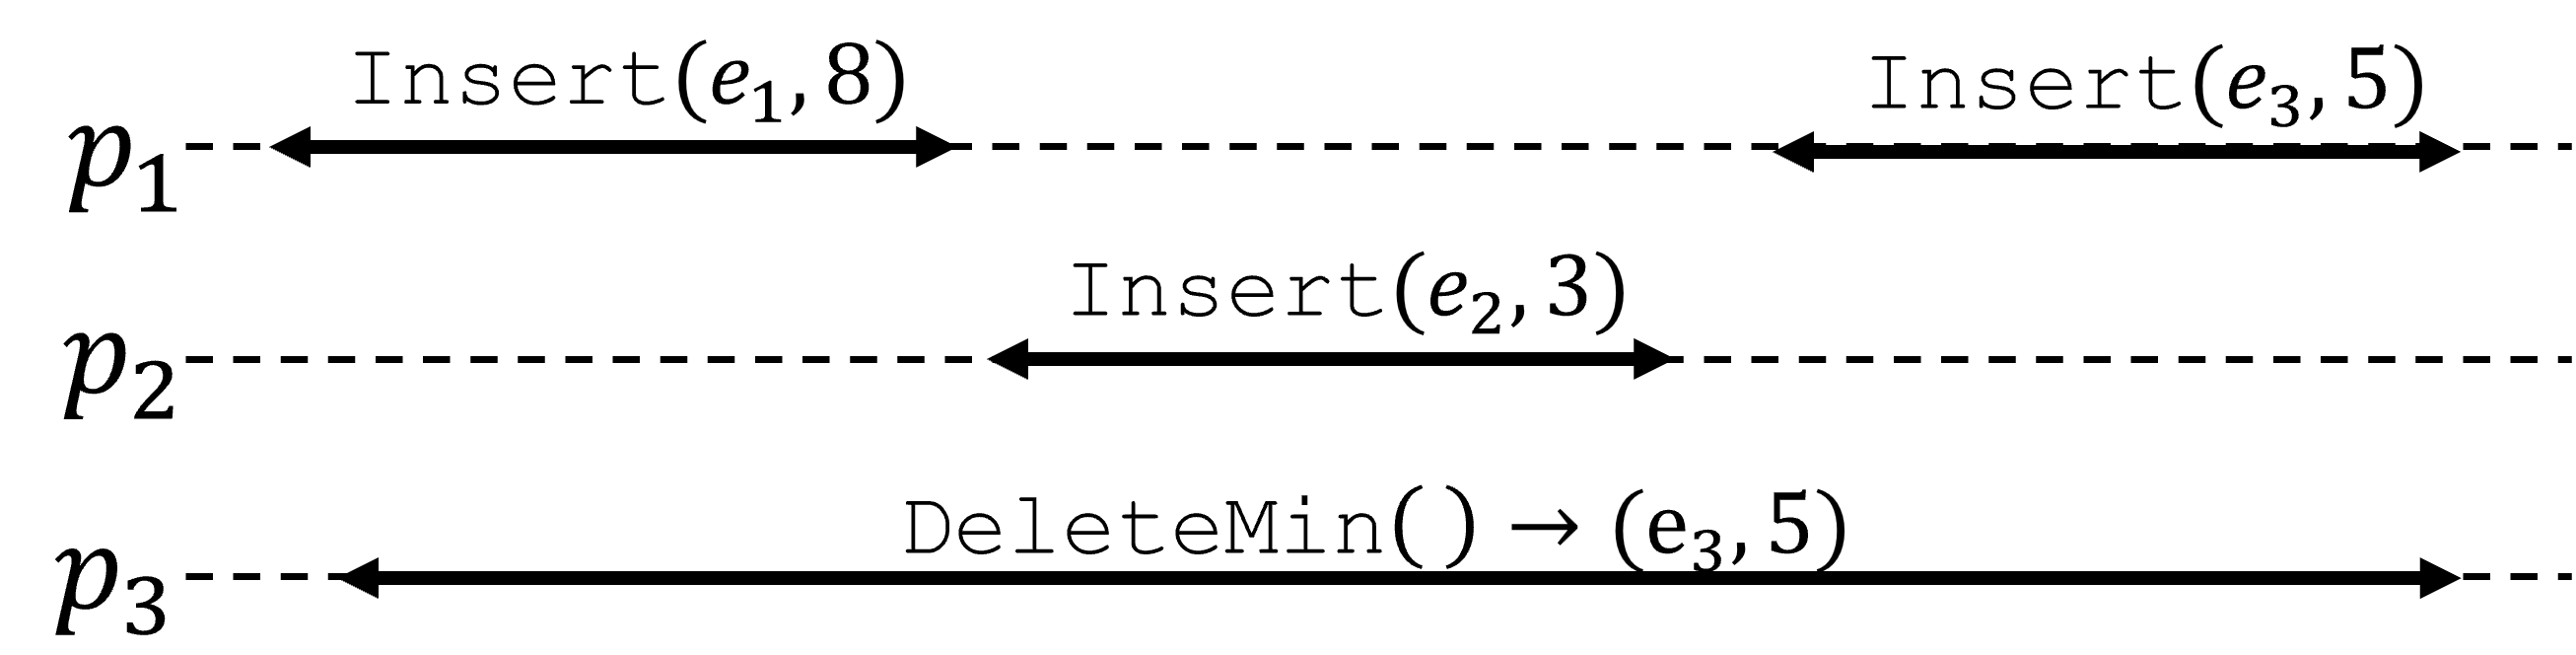
\includegraphics[width=0.4\textwidth]{graphics/ivl/PQIVLandSC.png}
  \caption{A possible concurrent history of a PQ that is both IVL and SC but not linearizable. The SC property requires that the remove be of some previously inserted element, and the IVL property requires that the element have a priority bound between $8$ and $3$.}
  \label{ivl-fig:SC-IVL-and-SC}
\end{figure}


\section{Lower bound for linearizable batched counter}
\label{ivl-ssec:lower-bound}

The incentive for using an IVL batched counter instead of a linearizable one stems
from a lower bound on the step-complexity of a wait-free linearizable batched counter implementation from SWMR registers.
To show the lower bound we first define the binary snapshot object.
A \emph{snapshot object} has $n$ components written by separate processes, and allows a reader to
capture the shared variable states of all $n$ processes instantaneously. We
consider the \emph{binary snapshot object}, in which each state component may be either $0$ or $1$~\cite{hoepman1993binary}. The object
supports the {\sc update}$_i$($v$) and {\sc scan} operations, where the former sets the state of component $i$
to value $v \in \{0,1\}$ and the latter returns all processes states instantaneously.
It is trivial that the {\sc scan} operation must read all states, therefore its lower bound step complexity
is $\Omega(n)$. Israeli and Shriazi~\cite{israeli1998time} show that the {\sc update} step complexity
of any implementation of a snapshot object from SWMR registers is also $\Omega(n)$. This lower bound
was shown to hold also for multi writer registers~\cite{attiya2006complexity}. While
their proof was originally given for a multi value snapshot object, it holds in the binary case as well~\cite{hoepman1993binary}.

\begin{algorithm}
    \begin{algorithmic}[1]
        % \begin{multicols}{2}

        \State local variable $v_i$ \Comment{Initialized to $0$}
        \State shared batched counter object $\mathit{BC}$ \Comment{Initialized to $0$}
        \Statex
        \Procedure{update$_i$}{$v$}
        \State \algorithmicif\ $v_i = v$\ \algorithmicthen\ \textbf{return} \label{ivl-l:skip}
        \State $v_i \gets v$
        \State \algorithmicif\ $v = 1$\ \algorithmicthen\ $\mathit{BC}$.{\sc update}$_i$($2^i$) \label{ivl-l:set-1}
        \State \algorithmicif\ $v = 0$\ \algorithmicthen\ $\mathit{BC}$.{\sc update}$_i$($2^n - 2^i$) \label{ivl-l:set-0}
        \EndProcedure
        % \columnbreak
        \Procedure{scan}{}
        \State $\mathit{sum} \gets \mathit{BC}$.{\sc read}() \label{ivl-l:read} % $\mod 2^n$
        \State $v[0 \dots n-1] \gets [0 \dots 0]$ \Comment{Initialize an array of $0$'s}
        \For{$i : 0 \leq i \leq n-1$}
        \State \algorithmicif\ bit $i$ is set in $\mathit{sum}$\ \algorithmicthen\ $v[i] \gets 1$ \label{ivl-l:check-set}
        \EndFor
        \State \textbf{return} $v[0 \dots n-1]$
        \EndProcedure
    % \end{multicols}
    \end{algorithmic}
    \caption{Algorithm for process $p_i$, solving binary snapshot with a batched counter object.}
    \label{ivl-alg:bs-with-adder}
\end{algorithm}

To show a lower bound on the {\sc update} operation of wait-free linearizable batched counters,
we show a reduction from a binary snapshot to a batched counter in
Algorithm~\ref{ivl-alg:bs-with-adder}. It uses a local variable $v_i$ and a shared batched counter object.
In a nutshell, the idea is to encode the value of the $i^\text{th}$ component
of the binary snapshot using the $i^\text{th}$ least significant bit of the counter.
When the component changes from $0$ to $1$, {\sc update}$_i$ adds $2^i$, and when it changes from $1$ to $0$,
{\sc update}$_i$ adds $2^n - 2^i$. We now prove the following invariant:
\begin{invariant}
    \inred{For any prefix $H'$ of $H$ of length $t$} of a sequential execution of Algorithm~\ref{ivl-alg:bs-with-adder},
    the sum held by the counter is $c \cdot 2^n + \sum_{i=0}^{n-1}v_i2^i$,
    such that $v_i$ is the parameter passed to the last invocation of {\sc update}$_i$ in $H'$ if such invocation
    exists, and $0$ otherwise, for some integer $c \in \mathbb{N}$.
    \label{ivl-inv:sum}
\end{invariant}
\begin{proof}
    We prove the invariant by induction on the length of $H$, i.e., the number of invocations in $H$,
    denoted $t$. As $H$ is a sequential history, each invocation is followed by a response.
    %\par{\textbf{Base:}}
    The base if for $t=0$, i.e., $H$ is the empty execution. In this case no updates
    have been invoked, therefore $v_i=0$ for all $0 \leq i \leq n-1$. The sum returned by the counter
    is $0$. Choosing $c=0$ satisfies the invariant.
    %\par{\textbf{Induction step:}}
    Our induction hypothesis is that the invariant holds for a history of length $t$.
    We prove that it holds for a history of length $t+1$. The last invocation can be either a {\sc scan}, or an {\sc update}($v$)
    by some process $p_i$. If it is a {\sc scan}, then the counter value doesn't change and the invariant
    holds. Otherwise, it is an {\sc update}($v$). Here, we note two cases. Let $v_i$ be $p_i$'s value
    prior to the {\sc update}($v$) invocation. If $v = v_i$, then the {\sc update} returns without altering the sum
    and the invariant holds. Otherwise, $v \neq v_i$. We analyze two cases, $v=1$ and $v=0$. If $v=1$, then $v_i=0$.
    The sum after the update is $c \cdot 2^n + \sum_{i=0}^{n-1}v_i2^i + 2^i=c \cdot 2^n + \sum_{i=0}^{n-1}v_i'2^i$, where
    $v_j'=v_j$ if $j \neq i$, and $v'_i = 1$, and the invariant holds. If $v=0$, then $v_i=1$.
    The sum after the update is $c \cdot 2^n + \sum_{i=0}^{n-1}v_i2^i + 2^n - 2^i = (c+1) \cdot 2^n + \sum_{i=0}^{n-1}v_i'2^i$,
    where $v_j'=v_j$ if $j \neq i$, and $v'_i = 1$, and the invariant holds.
\end{proof}

Using the invariant, we prove the following lemma:
\begin{lemma}
    For any sequential history $H$, if a {\sc scan} returns $v_i$, and {\sc update}$_i$($v$) is the last update invocation in $H$
    prior to the {\sc scan}, then $v_i = v$. If no such update exists, then $v_i=0$.
    \label{ivl-lmma:scan-correctness}
\end{lemma}
\begin{proof}
    Let $S$ be a {\sc scan} in $H'$. Consider the sum $\textit{sum}$ as read by scan $S$.
    From Invariant~\ref{ivl-inv:sum}, the value held by the counter is $c \cdot 2^n + \sum_{i=0}^{n-1}v_i2^i$.
    There are two cases, either there is an update invocation prior to $S$, or there isn't. If there isn't, then by
    Invariant~\ref{ivl-inv:sum} the corresponding $v_i=0$. The process sees bit $i=0$,
    and will return $0$. Therefore, the lemma holds.

    Otherwise, there is a an update prior to $S$ in $H$. As the sum is equal to $c \cdot 2^n + \sum_{i=0}^{n-1}v_i2^i$,
    by Invariant~\ref{ivl-inv:sum}, bit $i$ is equal to $1$ iff the parameter passed to the last invocation of update was $1$.
    Therefore, the scan returns the parameter of the last update and the lemma holds.
\end{proof}

\begin{lemma}
    Algorithm~\ref{ivl-alg:bs-with-adder} implements a linearizable binary snapshot using a linearizable batched counter.
    \label{ivl-lmma:reduction}
\end{lemma}
\begin{proof}
    Let $H$ be a history of Algorithm~\ref{ivl-alg:bs-with-adder}, and let $H'$ \inred{be the subset of operations in $H$ that
    access the linearizable batched counter (and removed otherwise),}
    where each operation is linearized at its access to the linearizable batched counter \inred{with responses added to
    pending operations}, or
    its response if $v_i = v$ on line~\ref{ivl-l:skip}.
    Applying Lemma~\ref{ivl-lmma:scan-correctness} to $H'$, we get $H' \in \mathcal{H}$ and therefore $H$ is linearizable.
\end{proof}

It follows from the algorithm that if the counter
object is bounded wait-free then the {\sc scan} and {\sc update} operations are bounded wait-free. Therefore, the lower
bound proved by Israeli and Shriazi~\cite{israeli1998time} holds, and the {\sc update} must take $\Omega(n)$
steps. Other than the access to the counter in the {\sc update} operation, it takes
$O(1)$ steps. Therefore, the access to the counter object must take $\Omega(n)$ steps. We have proven the following theorem.
\begin{theorem}
    For any linearizable wait-free implementation of a batched counter object with $n$ processes from SWMR registers, the step-complexity
    of the {\sc update} operation is $\Omega(n)$.
    \label{ivl-thm:lower-bound}
\end{theorem}


\section{Conclusion}
\label{ivl-sec:conclusion}

We have presented IVL, a new correctness criterion that provides flexibility
in the return values of quantitative objects while bounding the error that this may
introduce. IVL has a number of desirable properties: First,
like linearizability, it is a local property, allowing designers to reason about each part
of the system separately. Second, also like linearizability but unlike other relaxations of
it, IVL preserves the error bounds of PAC objects. Third, IVL is generically defined for
all quantitative objects, and does not necessitate object-specific definitions. Finally,
IVL is inherently amenable to cheaper implementations than linearizability in some cases.

Via the example of a CountMin sketch, we have illustrated that IVL provides
a generic way to efficiently parallelize data sketches while leveraging their
sequential error analysis to bound the error in the concurrent implementation.

We have shown that IVL can also capture the semantics of non-atomic snapshots,
by augmenting the data structure with an auxiliary history
variable. Finally, we have shown that sometimes IVL is useful
in tandem with other correctness criteria via the
example of a priority queue, where we pair IVL with sequential consistency.

The notion of IVL raises a main question for future research:
In this work we have shown that IVL is a sufficient condition for parallel
$(\epsilon,\delta)$-bounded objects, in that it preserves their sequential
error. It would be interesting to investigate whether IVL is also necessary,
or whether some weaker condition is sufficient.

\chapter{Compressing Distributed Network Sketches with  Traffic-Aware Summaries}
\label{chap:sktc}

\section{Introduction}\label{sktc-sec:intro}
Network designers need to gather analytics about the performance of the network to better understand what is happening behind the curtain. 
\ingreen{These are useful for traffic engineering, 
for reaching a higher utilization of the infrastructure,
for reducing link congestion, and for detecting anomalies when they happen.} Switches generally do not have sufficient memory to hold entire measurement models for large data streams, therefore the network designer generally sacrifices accuracy for a lower memory footprint.
Data sketching algorithms, or \textit{sketches} for short \cite{cormode2012synopses}, are
an indispensable tool for such high-speed low-memory-footprint computations. Sketches  estimate some function
of a large stream \ingreen{such as} \inblue{flow sizes}~\cite{CountMin} (i.e., the number of packets in a flow), \inblue{stream cardinality}~\cite{datar2002comparing, flajolet1983probabilistic} (i.e., the number of flows in a stream), the top-$k$ most common items~\cite{metwally2005efficient} or  frequency changes~\cite{IMCBal03}.
They are supported by many data analytics platforms such as PowerDrill~\cite{heule2013hyperloglog},
Druid~\cite{druid}, Hillview~\cite{hillview}, and Presto~\cite{presto} as well as \ingreen{by} standalone toolkits~\cite{apache-datasketches}.


Measurements are conducted in switches  all over the network; however, to successfully analyze network behavior, measurement data needs to be gathered in a centralized server that can see \ingreen{a wider view}.
\forRevThree{A stream of multiple flows passes through the network, with disjoint parts of the stream sampled by multiple \emph{ingestion nodes}, where parts of the same flow may be ingested by different nodes. The ingestion nodes periodically propagate their local sketch to a \emph{central node}, as illustrated in Figure~\ref{sktc-fig:ingestion-nodes}.  The network has to handle the trade-off of sending data packets vs. sending crucial control packets with sketch information~\cite{zhang2010optimizing, %zhang2009spatio,
benson2010understanding}. A way to reduce these control packets is by compressing the sketches before transferring them to a central analytics node.}



%\inred{To capture this behavior, we treat all of the incoming packets to the network as originating from a single \emph{stream}, which consists of multiple \emph{flows}.}
%\inblue{The stream is split into disjoint parts observed by multiple \emph{ingestion nodes}. Parts of the same flow may be ingested by different nodes.}  Once the nodes have a sketch ready to be sent (e.g., they periodically receive a packet signaling the end of their current stream and start a new one) they propagate their local sketch to a \emph{central node}~\cite{huang2017sketchvisor, li2016flowradar, liu2016one}. This is illustrated in Figure~\ref{sktc-fig:ingestion-nodes}. The network has to handle the trade-off of sending data packets vs. sending crucial control packets~\cite{zhang2010optimizing, %zhang2009spatio,
%benson2010understanding} with sketch information. A way to reduce these control packets is by compressing the sketches before transferring them to a central analytics node. 

\inblue{Compressing is crucial as network managers may have many sketches estimating different measurements concurrently. While each sketch alone may be insignificant, their aggregate is noticeable at the network level. Additionally, the sketch may be collecting measurements in low bandwidth networks~\cite{muthitacharoen2001low, margaritis2003peer}}, \ingreen{making the sketch size critical.}


\begin{figure}
    \centering
    %\includegraphics[width=0.9\linewidth]{figures/IngestionNodesPic.png}
    \tikzset{every picture/.style={line width=0.75pt}} %set default line width to 0.75pt    
    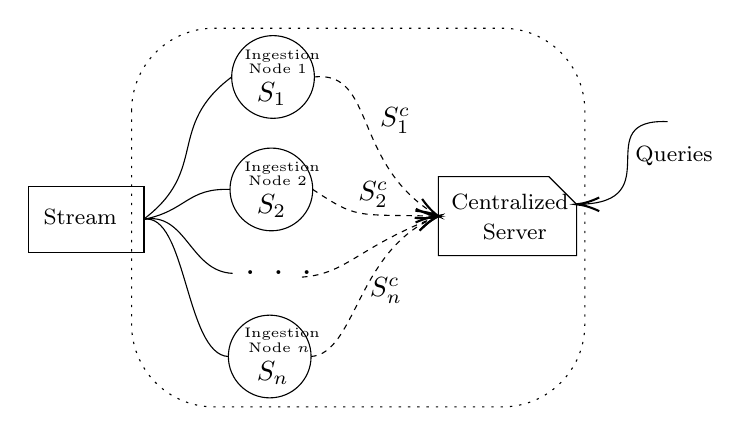
\begin{tikzpicture}[x=0.75pt,y=0.75pt,yscale=-1,xscale=1]
    %uncomment if require: \path (0,300); %set diagram left start at 0, and has height of 300
    
    %Shape: Rectangle [id:dp7800934124171983] 
    \draw   (117,155.65) -- (172.78,155.65) -- (172.78,187.53) -- (117,187.53) -- cycle ;
    %Shape: Ellipse [id:dp20814509523202052] 
    \draw   (215.02,103.05) .. controls (215.02,92.05) and (223.94,83.13) .. (234.94,83.13) .. controls (245.95,83.13) and (254.87,92.05) .. (254.87,103.05) .. controls (254.87,114.06) and (245.95,122.98) .. (234.94,122.98) .. controls (223.94,122.98) and (215.02,114.06) .. (215.02,103.05) -- cycle ;
    %Shape: Ellipse [id:dp5192677502317808] 
    \draw   (214.22,157.24) .. controls (214.22,146.24) and (223.14,137.32) .. (234.15,137.32) .. controls (245.15,137.32) and (254.07,146.24) .. (254.07,157.24) .. controls (254.07,168.25) and (245.15,177.17) .. (234.15,177.17) .. controls (223.14,177.17) and (214.22,168.25) .. (214.22,157.24) -- cycle ;
    %Shape: Circle [id:dp7676828342293531] 
    \draw   (213.43,237.73) .. controls (213.43,226.73) and (222.35,217.81) .. (233.35,217.81) .. controls (244.35,217.81) and (253.27,226.73) .. (253.27,237.73) .. controls (253.27,248.74) and (244.35,257.66) .. (233.35,257.66) .. controls (222.35,257.66) and (213.43,248.74) .. (213.43,237.73) -- cycle ;
    %Snip Single Corner Rect [id:dp7350487709437881] 
    \draw   (314.63,151.1) -- (367.87,151.1) -- (381.18,164.41) -- (381.18,189.12) -- (314.63,189.12) -- cycle ;
    %Curve Lines [id:da7243599111171348] 
    \draw   [dash pattern={on 2pt off 2pt}]   (254.87,103.05) .. controls (284.45,99.9) and (273.03,145.17) .. (313.4,169.38) ;
    \draw [shift={(314.63,170.11)}, rotate = 209.86] [color={rgb, 255:red, 0; green, 0; blue, 0 }  ][line width=0.75]    (10.93,-3.29) .. controls (6.95,-1.4) and (3.31,-0.3) .. (0,0) .. controls (3.31,0.3) and (6.95,1.4) .. (10.93,3.29)   ;
    %Curve Lines [id:da4335557046839309] 
    \draw   [dash pattern={on 2pt off 2pt}]   (254.07,157.24) .. controls (275.66,171.37) and (273.66,169.27) .. (312.82,170.07) ;
    \draw [shift={(314.63,170.11)}, rotate = 181.27] [color={rgb, 255:red, 0; green, 0; blue, 0 }  ][line width=0.75]    (10.93,-3.29) .. controls (6.95,-1.4) and (3.31,-0.3) .. (0,0) .. controls (3.31,0.3) and (6.95,1.4) .. (10.93,3.29)   ;
    %Curve Lines [id:da47273415849462186] 
    \draw   [dash pattern={on 2pt off 2pt}]   (253.27,237.73) .. controls (274.86,236.16) and (275.18,186.66) .. (312.89,170.81) ;
    \draw [shift={(314.63,170.11)}, rotate = 519.15] [color={rgb, 255:red, 0; green, 0; blue, 0 }  ][line width=0.75]    (10.93,-3.29) .. controls (6.95,-1.4) and (3.31,-0.3) .. (0,0) .. controls (3.31,0.3) and (6.95,1.4) .. (10.93,3.29)   ;
    %Curve Lines [id:da7986835200568454] 
    \draw   [dash pattern={on 2pt off 2pt}]   (248.89,199.48) .. controls (270.48,197.91) and (275.05,185.52) .. (312.88,170.78) ;
    \draw [shift={(314.63,170.11)}, rotate = 519.15] [color={rgb, 255:red, 0; green, 0; blue, 0 }  ][line width=0.75]    (10.93,-3.29) .. controls (6.95,-1.4) and (3.31,-0.3) .. (0,0) .. controls (3.31,0.3) and (6.95,1.4) .. (10.93,3.29)   ;
    %Rounded Rect [id:dp16891083296577403] 
    \draw  [dash pattern={on 0.84pt off 2.51pt}] 
    (166.81,119.26) .. controls (166.81,97.34) and (184.58,79.57) .. (206.49,79.57) -- (345.47,79.57) .. controls (367.39,79.57) and (385.16,97.34) .. (385.16,119.26) -- 
    %(166.81,113.26) .. controls (166.81,91.34) and (184.58,73.57) .. (206.49,73.57) -- (345.47,73.57) .. controls (367.39,73.57) and (385.16,91.34) .. (385.16,113.26) -- 
    %(385.16,232.31) .. controls (385.16,254.23) and (367.39,272) .. (345.47,272) -- (206.49,272) .. controls (184.58,272) and (166.81,254.23) .. (166.81,232.31) -- cycle ;
    (385.16,222.31) .. controls (385.16,244.23) and (367.39,262) .. (345.47,262) -- (206.49,262) .. controls (184.58,262) and (166.81,244.23) .. (166.81,222.31) -- cycle ;
    
    %Curve Lines [id:da7483451131891823] 
    \draw    (172.5,171.67) .. controls (204.38,147.76) and (183.14,126.96) .. (215.02,103.05) ;
    %Curve Lines [id:da3567735385248336] 
    \draw    (172.5,171.67) .. controls (193.22,167.68) and (193.5,156.45) .. (214.22,157.24) ;
    %Curve Lines [id:da8413889792937872] 
    \draw    (172.5,171.67) .. controls (193.22,167.68) and (194.78,196.87) .. (215.5,197.67) ;
    %Curve Lines [id:da820436037263437] 
    \draw    (172.5,171.67) .. controls (193.22,167.68) and (192.71,236.94) .. (213.43,237.73) ;
    %Curve Lines [id:da6059682612620094] 
    \draw    (425.01,124.57) .. controls (386.35,122.99) and (426.58,163.59) .. (382.54,164.39) ;
    \draw [shift={(381.18,164.41)}, rotate = 360.01] [color={rgb, 255:red, 0; green, 0; blue, 0 }  ][line width=0.75]    (10.93,-3.29) .. controls (6.95,-1.4) and (3.31,-0.3) .. (0,0) .. controls (3.31,0.3) and (6.95,1.4) .. (10.93,3.29)   ;
    
    % Text Node
    \draw (123.1,165.49) node [anchor=north west][inner sep=0.75pt]  [font=\footnotesize] [align=left] {Stream};
    % Text Node
    \draw (219.94,88.66) node [anchor=north west][inner sep=0.75pt]   [align=left] {{\tiny Ingestion}};
    \draw (221.94,95.66) node [anchor=north west][inner sep=0.75pt]   [align=left] {{\tiny Node 1}};
    \draw (225.94,104.66) node [anchor=north west][inner sep=0.75pt]   [align=left] {\textit{$S_1$}};
    % Text Node
    \draw (219.84,142.65) node [anchor=north west][inner sep=0.75pt]   [align=left] {{\tiny Ingestion }};
    \draw (221.84,149.65) node [anchor=north west][inner sep=0.75pt]   [align=left] {{\tiny Node 2}};
    \draw (225.84,158.55) node [anchor=north west][inner sep=0.75pt]   [align=left] {\textit{$S_2$}};
    % Text Node
    \draw (219.84,222.73) node [anchor=north west][inner sep=0.75pt]   [align=left] {{\tiny Ingestion }};
    \draw (221.84,229.73) node [anchor=north west][inner sep=0.75pt]   [align=left] {{\tiny Node $n$}};
    \draw (225.84,238.73) node [anchor=north west][inner sep=0.75pt]   [align=left] {\textit{$S_n$}};
    % Text Node
    \draw (319.63,158.1) node [anchor=north west][inner sep=0.75pt]  [font=\small] [align=left] {{\footnotesize Centralized }\\{\footnotesize  \ \ \ \ Server}};
    % Text Node
    \draw (285.31,116.67) node [anchor=north west][inner sep=0.75pt]   [align=left] {\textit{$S^c_1$}};%{\textit{S{\tiny 1}}};
    % Text Node
    \draw (274.76,152.33) node [anchor=north west][inner sep=0.75pt]   [align=left] {\textit{$S^c_2$}};
    % Text Node
    \draw (280.34,198.55) node [anchor=north west][inner sep=0.75pt]   [align=left] {\textit{$S^c_n$}};
    % Text Node
    \draw (220.15,195.31) node [anchor=north west][inner sep=0.75pt]   [align=left] {{\Large . . .}};
    % Text Node
    \draw (408.29,135.38) node [anchor=north west][inner sep=0.75pt]  [font=\footnotesize] [align=left] {Queries};
    
    \end{tikzpicture}
    \caption{Network-wide measurement over $n$ ingestion nodes: Queries are answered by  a centralized server collecting summaries $S^c_1, \ldots, S^c_n$ of the local sketches $S_1, \ldots, S_n$ (e.g., the Count-Min sketch (CM) or the K-minimum-values (KMV) sketch) in the ingestion nodes.}
    \label{sktc-fig:ingestion-nodes}
\end{figure}

A framework for sketch compression was suggested by Yang et al.~\cite{yang2018elastic}. A major component of this framework, named \emph{Maximum Merging Algorithm (\textbf{MM})}, compresses a Count-Min sketch (CM) by utilizing a $\max$ function and merging multiple cells in one CM to generate a new, smaller sketch. 
The first limitation of that approach is that it compresses a sketch only into smaller sketches of particular sizes, those that have a common divisor with the size of the original sketch. Moreover, the approach does not provide insights for the selection of the various compression ratios that should be implied for a distributed measurement in multiple nodes. In particular, how the traffic distribution among the nodes should be considered. 
%However, this compression method has two issues we attempt to resolve.  We allow higher flexibility and propose a new method called CM-SKTC that supports compressing a CM to any size needed sketch. Our second contribution is that we suggest a traffic-aware compression method that considers the distribution among the ingestion nodes and allocates to each node the summary size it should report, such that a node that received a larger portion of the traffic sends a larger summary and vice versa.
 
A clear drawback of compression methods is the accuracy reduction they might imply. 
%However network managers want to have data that has some guarantees of its accuracy. 
It is often critical for network managers to have access to measurements with guarantees of their accuracy.
In the common case that the network has multiple ingestion nodes that generate the measurements and send the data to a centralized server, it is intuitive to allow each node to report them through an amount of data that is correlative to the amount of traffic it observes. In this paper,  \emph{we study distributed sketch-based network measurement with limited communication. For optimizing accuracy  we call for traffic-aware compression ratios of the multiple sketch instances.} We present a formal model that refers to any given number of ingestion nodes and any distribution of the traffic through these nodes. Moreover, the resize factors also guarantee that the amount of data  sent over the network is less than compressing all the data from all the nodes to the same size with previously presented methods.




We present the following major contributions: 

%\emph{(i)} We motivate a compression method for distributed measurement which is traffic aware. We focus on the CM and describe the traffic-aware Count-Min sketch, denoted TA-CM, that computes the ideal compression ratios for the various nodes for reducing the total amount of reported data. We provide guarantees on the error bounds of the approach.
\emph{(i)} As a building block, we develop a compression method named CM-SKTC for a single CM that allows general compression ratios, and then present the Traffic-Aware CM sketch, denoted TA-CM.



\emph{(ii)} We present Traffic-Aware K-minimum-values (KMV), denoted TA-KMV -- a traffic-aware compression ratio for nodes implementing distributed distinct flow count with the KMV sketch.

\inblue{
\emph{(iii)} Finally, we present Traffic-Aware HyperLogLog (HLL), denoted TA-HLL -- a traffic-aware compression ratio for nodes implementing distributed distinct flow count with the HLL sketch.
}


%\inblue{
%A preliminary version of this article %\inred{appeared} at IFIP Networking, Virtual %Conference, June 2021~\cite{IFIP21}. This submission %includes the following new technical contributions:}

%\inblue{
%(i) The proofs for Lemma 1 and Theorems 1 and 2 are %first presented here. Lemma 2 and its proof is also %first presented here.}

%\inblue{
%(ii) An extension of the traffic-aware approach to %the HyperLogLog sketch (Section II.C and Section %VI). Experimental results for this sketch appear in %the Section VII.E. 
%}

The rest of the paper is organized as follows. Section \ref{sktc-sec:background} discusses \forRevThree{preliminaries, our model,} and related work. In Section \ref{sktc-sec:com-sketch} we present the CM-SKTC compression method for a single CM, bound its error, and describe how to decrease the data sent from ingestion nodes to the centralized server. 
The TA-CM for traffic-aware CM compression for multiple nodes is described in Section~\ref{sktc-sec:resize}.  
Section~\ref{sktc-sec:kmv-sktc} presents the TA-KMV for cardinality estimation (count distinct). Experimental evaluation of the methods is provided in Section \ref{sktc-sec:evaluation}. Finally, in Section \ref{sktc-sec:conclusion} we conclude and suggest directions for future work.

\section{Preliminaries} \label{sktc-sec:background}
\forRevThree{In this section we present the model, as well as background on sketches. 
%and the Maximum Merging (MM) method~\cite{yang2018elastic} for compressing the CM sketch. 
Finally, we detail related work.
}

\forRevThree{
\subsection{Model}
}

\forRevThree{
We consider the incoming packets in the network as originating from a single \emph{stream}. A \emph{flow} is defined to be a sub-stream with common packet headers, e.g., grouping together all packets containing the same 5-tuple. A \emph{measurement} is some function $f$ computed over the stream, e.g., returning the distinct number of flows in the stream. As streams are generally too large to maintain in memory~\cite{cormode2011sketch}, accuracy is traded off for a lower memory footprint~\cite{CountMin, agarwal2013mergeable, KMV} by algorithms called \emph{sketches}. Several sketches have the \emph{mergeability} property that refers to the ability for computing a sketch over a stream by merging sketches over substreams.}

\forRevThree{
As mentioned previously, measurements are conducted in switches all over the network. We model this by splitting the stream into disjoint sub-streams observed by \emph{ingestion nodes}, where parts of the same flow may be observed by different ingestion nodes. Once the nodes have a sketch ready to be sent (e.g.,  periodically or upon receive a specific signal) they propagate their local sketch or a summary for it to a \emph{central node}~\cite{huang2017sketchvisor, li2016flowradar, liu2016one}, which merges all sketches to provide the desired measurement.}

\subsection{Background}

In this section, we present the Count-Min sketch, the KMV sketch, and the HLL sketch. We present the Maximum Merging (MM) method.

\subsubsection{The Count-Min Sketch (CM)} \label{sktc-ssec:backgroound-CM}

Estimating flow size is a required capability 
in many networking applications,
in fields as diverse as accounting, monitoring, load balancing and filtering, and even beyond networking. Counting the exact size of every flow is often challenging due to a typically large number of active flows at a specific time, making it difficult to maintain a counter-per-flow within a memory accessible at the line rate.
There can be two types of errors in the estimation of a flow size: Overestimations and underestimations. The state-of-the-art data structure for flow size estimation is the Count-Min (CM) sketch  suggested by Cormode and Muthukrishnan in 2005~\cite{CountMin}.

\forRevThree{The CM sketch is instantiated with parameters $\epsilon$ and $\delta$, where the flow size estimation is within error $\epsilon$ with probability at least $1-\delta$. It is comprised of a two dimensional} array of counters of size $d \times w$, where $d = \lceil \ln{1 / \delta}\rceil$ and $w=\lceil e / \epsilon \rceil$, and all counters are initialized to 0. Note that the number of columns is determined by the error (and, conversely, the error is determined by the number of columns), and the probability is determined by the number of rows.
A set of $d$ hash functions are used to map a flow to $d$ counters, one in each of its rows. 
Upon a flow arrival, each of these counters is incremented.

To estimate the size of a flow, its $d$ selected counters are considered and the size is estimated as the minimum among these counters. Since multiple flows can contribute to the same counter, the computed value is \ingreen{potentially} larger than the exact one. \ingreen{In case other flows contributed to all $d$ counters then an overestimation is derived}. 
CM completely avoids underestimations. A tradeoff exists between the level of accuracy and the allocated memory such that more memory reduces collisions among flows. Similarly, reducing the number of flows improves accuracy.

\inblue{An important property of the CM sketch is the \emph{mergeability} property: Two CM sketches with parameters $(\epsilon,\delta)$ can be merged by element-wise addition to a sketch with the same parameters.} \forRevThree{We capitalize on this property which enables computing a sketch over the whole stream by merging sketches over substreams, which has also been exploited in previous work~\cite{stylianopoulos2020delegation, rinberg2019fast, cormode2011algorithms}.}

 %However, to the best of our knowledge there are no known results on how to completely avoid flow size overestimations even when the number of flows is small.


\begin{figure}[!t]%[!ht]
	\centering
		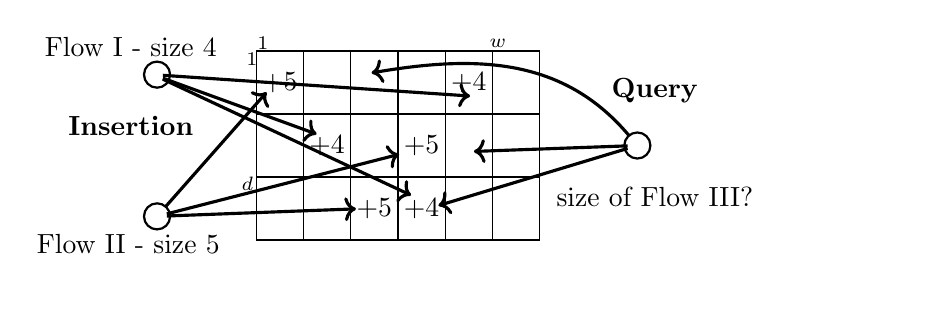
\begin{tikzpicture}
 \foreach \c/\i [count=\n] in  
        {white/4,white/0, white/0,white/0,white/9,white/0} 
           \node[draw,fill=\c,minimum height=0.8cm,minimum width = 0.6cm,xshift=(\n+2.1)*0.6cm](B\n){};
            \foreach \c/\i [count=\n] in  
        {white/4,white/0, white/0,white/0,white/9,white/0} 
           \node[draw,fill=\c,minimum height=0.8cm,minimum width = 0.6cm,xshift=(\n+2.1)*0.6cm, yshift =0.8cm](B\n){} ;
            \foreach \c/\i [count=\n] in 
        {white/4,white/0, white/0,white/0,white/9,white/0} 
           \node[draw,fill=\c,minimum height=0.8cm,minimum width = 0.6cm,xshift=(\n+2.1)*0.6cm, yshift =1.6cm](B\n){} ;
         \foreach \j [count=\m] in  
        {0,1,2,3,4,5,6,7,8,9,10,11,12,13,14} 
           \node[] (q\m) at (\m*0.5cm,0.36) {}; 
\node[text width=0.75cm, anchor=west, right] at (0.73,-1.0) {};
\node[text width=0.75cm, anchor=west, right] at (2.31,-1.0) {};
 \foreach \j [count=\m] in  
        {1,1,2,3,4,5,6,7,8,9,10,11,12} 
           \node[] (z\m) at (\m*0.5cm,-0.46) {}; 
\node[text width=3.5cm, anchor=west, right] at (-1.25,2.05) {Flow I - size 4};
\node[draw,circle,scale=1.0, thick] at (0.30,1.7) {}; 
\node [] (n0) at (0.25,1.7) {};
\node [] (z1) at (4.40,1.42) {};
\node [] (z2) at (2.45,0.9) {};
\node [] (z3) at (3.65,0.11) {};
\draw[line width=0.04cm, ->] (n0) -- (z1);
\draw[line width=0.04cm, ->] (n0) -- (z2);
\draw[line width=0.04cm, ->] (n0) -- (z3);

\node[text width=0.5cm, anchor=west, right] at (2.11,0.8) {$+4$};
\node[text width=0.5cm, anchor=west, right] at (3.91,1.6) {$+4$};
\node[text width=0.5cm, anchor=west, right] at (3.31,0.0) {$+4$};
\node[text width=0.5cm, anchor=west, right] at (2.71,0.0) {$+5$};
\node[text width=0.5cm, anchor=west, right] at (3.31,0.8) {$+5$};
\node[text width=0.5cm, anchor=west, right] at (1.51,1.6) {$+5$};
%\draw[->] (n0) -- (-0.4,+0.46);
%\draw[->] (n0) -- (q3);

\node[text width=0.5cm, anchor=west, right] at (1.45,2.10) {\scriptsize $1$};
\node[text width=0.5cm, anchor=west, right] at (4.40,2.10) {\scriptsize $w$};

\node[text width=0.5cm, anchor=west, right] at (1.31,1.90) {\scriptsize $1$};
\node[text width=0.5cm, anchor=west, right] at (1.25,0.32) {\scriptsize $d$};


\node[draw,circle,scale=1.0, thick] at (0.30,-0.1) {};
\node[text width=3.5cm, anchor=west, right] at (-1.35,-0.45) {Flow II - size 5};
\node [] (nl) at (0.30,-0.1) {};
\node [] (nl1) at (1.80,1.6) {};
\node [] (nl2) at (3.5,0.72) {};
\node [] (nl3) at (2.95,0.0) {};
\draw[line width=0.04cm, ->] (nl) -- (nl1);
\draw[ line width=0.04cm, ->] (nl) -- (nl2);
\draw[line width=0.04cm, ->] (nl) -- (nl3);


\node[draw,circle,scale=1.0, thick] at (6.40,0.8) {};
\node[text width=3.5cm, anchor=west, right] at (5.25,0.15) {size of Flow III?};
\node [] (n2) at (6.4,0.8) {};

\node [] (n21) at (2.90,1.7) {};
\node [] (n22) at (4.2,0.72) {}; 
\node [] (n23) at (3.75,0.0) {};
%\draw[blue, line width=0.04cm, ->] (n2) --  (n21);
\draw [->, line width=0.04cm] (n2) to [out=130,in=10] (n21);
\draw[line width=0.04cm, ->] (n2) -- (n22);
%\draw [->, line width=0.04cm] (n2) to [out=200,in=290] (n23);
\draw[line width=0.04cm, ->] (n2) -- (n23);
\node[text width=3.5cm, anchor=west, right] at (-0.95,1.05) {\textbf{Insertion}};
\node[text width=3.5cm, anchor=west, right] at (5.95,1.5) {\textbf{Query}};
%\draw[->] (nl) -- (q3);
%\draw[->] (nl) -- (q8);
%\node[text width=3.5cm, anchor=west, right] at (4.60,1.75) {Flow III - size 1};
%\node[draw,circle,scale=1.0, thick] at (5.29,1.4) {};
%\node [] (n2) at (5.3,1.3) {};
%\draw[->] (n2) -- (q8); 
%\draw[->] (n2) -- (q11); 
%\node[draw,circle,scale=1.0, thick] at (2.59,-1.4) {};
%\node[text width=4.0cm, anchor=west, right] at (1.51,-1.7) {size of Flow II?};
%\node [] (n3) at (2.6,-1.3) {};
%\draw[->] (n3) -- (z3);
%\draw[->] (n3) -- (z8);
\end{tikzpicture}
\caption{\label{sktc-fig:CM} The Count-Min sketch (CM)~\cite{CountMin}, allowing flow size estimation. \inred{Each flow is mapped to a single counter in each row. Flow I is mapped to counter 5 in row 1, counter 2 in row 2, and counter 4 in row 3. The mappings are presented in the figure.} A flow size is estimated as the minimum among the counters it is mapped to by a set of hash functions.}	
\end{figure}

The CM  is illustrated in Figure~\ref{sktc-fig:CM}. Flows I, II  of size 4, and 5, respectively, are recorded in the sketch (shown on the left side). Each flow increases the value of $d=3$ counters by its size.  The size of Flow III (right side) is estimated by querying the CM  as the minimal among the $d$ counters it is mapped to.

%As for every sketch, the estimation generated from the Count-Min sketch is imperfect and can be overestimated.
\inred{While, as mentioned, the CM can observe overestimations~\cite{CountMin}}, the accuracy guarantees can be described as follows:
When using CM with width $w$ and depth $d$ the estimation $\hat{f}$ of flow $f$ satisfies with probability $1-\delta$
\[\hat{f} \leq f + \epsilon N.\]
Here, $N$ is the number of packets in the measured stream, $\epsilon$ holds $w = \left\lceil \frac{e}{\epsilon} \right\rceil$ (for Euler's number $e$) and $\delta$ holds $d= \left\lceil \ln\frac{1}{\delta} \right\rceil$.

\subsubsection{KMV (\emph{K-minimum-values}) Sketch}  \label{sktc-ssec:kmv}

Another essential capability in network monitoring is the ability to estimate the number of distinct flows, called stream cardinality. Counting the exact stream cardinality is generally challenging in high traffic rate, making it hard to save some unique data for each flow and quickly identify whether a flow has previously appeared or not. 

The $K$-minimum-values sketch (KMV)~\cite{giroire2009order, KMV} uses a hash function $h$ that maps every flow uniformly to $[0,1]$. For a parameter $k$, the sketch maintains the minimal $k$ observed values for flows so far. Let $h_1,...,h_k$ be those $k$ minimal calculated values such that $h_1<h_2<...<h_k$. The \emph{KMV} sketch provides its cardinality estimation as $\frac{k}{h_k}$. This estimation is based on the fact that the $k$ order statistics of group uniformly randomized in the range $[0,1]$ is equal to $\frac{k}{n+1}$. The error of the algorithm is $\frac{1}{\sqrt{k}}$, i.e.  for $m$ flows, the KMV sketch estimation $m'$ satisfies $\left|\frac{m-m'}{m}\right| = O(\frac{1}{\sqrt{k}})$.

\begin{figure}[!t]%[!ht]
	\centering
	

\tikzset{every picture/.style={line width=0.75pt}} %set default line width to 0.75pt        

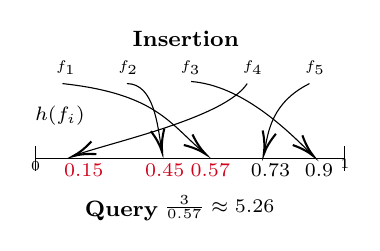
\begin{tikzpicture}[x=0.75pt,y=0.75pt,yscale=-1,xscale=1]
%uncomment if require: \path (0,300); %set diagram left start at 0, and has height of 300

%Straight Lines [id:da2080794547555267] 
\draw    (101.5,100.67) -- (250.5,100.67) ;
%Straight Lines [id:da6803929792177787] 
\draw    (101.5,94.67) -- (101.5,106.67) ;
%Straight Lines [id:da0782789730692306] 
\draw    (250.5,94.67) -- (250.5,106.67) ;
%Curve Lines [id:da9195899812176473] 
\draw    (114.5,64.67) .. controls (159.12,69.52) and (166.1,83.78) .. (182,97.4) ;
\draw [shift={(183.5,98.67)}, rotate = 219.47] [color={rgb, 255:red, 0; green, 0; blue, 0 }  ][line width=0.75]    (10.93,-3.29) .. controls (6.95,-1.4) and (3.31,-0.3) .. (0,0) .. controls (3.31,0.3) and (6.95,1.4) .. (10.93,3.29)   ;
%Curve Lines [id:da2342594252069674] 
\draw    (145.5,64.67) .. controls (158.66,64.67) and (160.33,84.99) .. (162.15,95.73) ;
\draw [shift={(162.5,97.67)}, rotate = 258.69] [color={rgb, 255:red, 0; green, 0; blue, 0 }  ][line width=0.75]    (10.93,-3.29) .. controls (6.95,-1.4) and (3.31,-0.3) .. (0,0) .. controls (3.31,0.3) and (6.95,1.4) .. (10.93,3.29)   ;
%Curve Lines [id:da7520327389763415] 
\draw    (176.5,63.67) .. controls (200.63,65.6) and (221.96,86.15) .. (234.2,98.37) ;
\draw [shift={(235.5,99.67)}, rotate = 225] [color={rgb, 255:red, 0; green, 0; blue, 0 }  ][line width=0.75]    (10.93,-3.29) .. controls (6.95,-1.4) and (3.31,-0.3) .. (0,0) .. controls (3.31,0.3) and (6.95,1.4) .. (10.93,3.29)   ;
%Curve Lines [id:da8707723296036518] 
\draw    (203.5,64.67) .. controls (192.89,81.07) and (138.5,92.82) .. (121.23,99.01) ;
\draw [shift={(119.5,99.67)}, rotate = 338.2] [color={rgb, 255:red, 0; green, 0; blue, 0 }  ][line width=0.75]    (10.93,-3.29) .. controls (6.95,-1.4) and (3.31,-0.3) .. (0,0) .. controls (3.31,0.3) and (6.95,1.4) .. (10.93,3.29)   ;
%Curve Lines [id:da46923256267070834] 
\draw    (233.5,64.67) .. controls (215,73.92) and (213.61,88.3) .. (211.93,96.74) ;
\draw [shift={(211.5,98.67)}, rotate = 284.04] [color={rgb, 255:red, 0; green, 0; blue, 0 }  ][line width=0.75]    (10.93,-3.29) .. controls (6.95,-1.4) and (3.31,-0.3) .. (0,0) .. controls (3.31,0.3) and (6.95,1.4) .. (10.93,3.29)   ;

% Text Node
\draw (98,101) node [anchor=north west][inner sep=0.75pt]   [align=left] {{\tiny 0}};
% Text Node
\draw (247,100) node [anchor=north west][inner sep=0.75pt]   [align=left] {{\tiny 1}};
% Text Node
\draw (110,52.4) node [anchor=north west][inner sep=0.75pt]  [font=\tiny]  {${\displaystyle f_{1}}$};
% Text Node
\draw (140,52.4) node [anchor=north west][inner sep=0.75pt]  [font=\tiny]  {${\displaystyle f_{2}}$};
% Text Node
\draw (170,52.4) node [anchor=north west][inner sep=0.75pt]  [font=\tiny]  {${\displaystyle f_{3}}$};
% Text Node
\draw (200,52.4) node [anchor=north west][inner sep=0.75pt]  [font=\tiny]  {${\displaystyle f_{4}}$};
% Text Node
\draw (230,52.4) node [anchor=north west][inner sep=0.75pt]  [font=\tiny]  {${\displaystyle f_{5}}$};
% Text Node
\draw (147,38) node [anchor=north west][inner sep=0.75pt]   [align=left] {\textbf{{\footnotesize Insertion}}};
% Text Node
\draw (230,102) node [anchor=north west][inner sep=0.75pt]   [align=left] {{\scriptsize 0.9}};
% Text Node
\draw (204,102) node [anchor=north west][inner sep=0.75pt]   [align=left] {{\scriptsize 0.73}};
% Text Node
\draw (175,102) node [anchor=north west][inner sep=0.75pt]  [color={rgb, 255:red, 208; green, 2; blue, 27 }  ,opacity=1 ] [align=left] {{\scriptsize 0.57}};
% Text Node
\draw (114,102) node [anchor=north west][inner sep=0.75pt]  [color={rgb, 255:red, 208; green, 2; blue, 27 }  ,opacity=1 ] [align=left] {{\scriptsize 0.15}};
% Text Node
\draw (153,102) node [anchor=north west][inner sep=0.75pt]  [color={rgb, 255:red, 208; green, 2; blue, 27 }  ,opacity=1 ] [align=left] {{\scriptsize 0.45}};
% Text Node
\draw (100,74.4) node [anchor=north west][inner sep=0.75pt]  [font=\scriptsize]  {$h( f_{i})$};
% Text Node
\draw (124,120) node [anchor=north west][inner sep=0.75pt]   [align=left] {\textbf{{\footnotesize Query}}};
% Text Node
\draw (162,117.4) node [anchor=north west][inner sep=0.75pt]  [font=\scriptsize]  {$\frac{3}{0.57} \approx 5.26$};


\end{tikzpicture}

    \caption{The $K$-minimum-values sketch (KMV) \cite{giroire2009order, KMV}, allowing cardinality estimation. The cardinality is estimated by dividing $k$ with the $k$'th minimal hashed value, (here $k=3$ with recorded values shown in red).}
    \label{sktc-fig:kmv-example}
\end{figure}

The KMV is illustrated in Figure \ref{sktc-fig:kmv-example}. There are five flows recorded in the sketch, each maps to a different value in the range of $[0,1]$. Here $k=3$ so that only the three minimal values are stored. When flows' cardinality is queried, the sketch finds the largest value that is currently stored, which is $0.57$ and returns $\frac{k}{0.57} = \frac{3}{0.57} \approx 5.26$ distinct flows.

\subsubsection{HyperLogLog for Cardinality Estimation}
\label{sktc-ssec:HyperLogLog}

% \begin{algorithm}[!h]
% \DontPrintSemicolon
% \KwIn{
% Stream of elements $A = (a_1, \ldots, a_k)$.
% }
% \KwOut{
% Estimated number of distinct elements in $A$
% }
% $M[0] = \ldots = M[m-1] = 0$, $d= \log_2(m)$, $\alpha_m  = 0.7213 / (1+1.079/m)$ for $m \ge 128$;

% \For{$a_i \in A$} {
% $(b_1, \ldots, b_d, b_{d+1}, \ldots, b_{d+t}) = h(a_i)$ \\
% $j =  (b_1, \ldots, b_d)$\\
% $M[j] = \max(M[j], \rho((b_{d+1}, \ldots, b_{d+t})))$
% }
% $Z = \Big(\sum_{j = 0}^{m-1} {2^{-M[j]}}\Big)^{-1}$\\
% \Return $\alpha_m  \cdot m^2 \cdot Z$\\
% \caption{The \emph{HyperLogLog} algorithm for cardinality estimation~\cite{Flajolet07hyperloglog}}
% %for estimating number of distinct elements
% \label{sktc-Alg_HyperLogLog}
% \end{algorithm}



HyperLogLog (HLL)~\cite{Flajolet07hyperloglog,heule2013hyperloglog} is another popular algorithm for cardinality estimation.
As a building block, it relies on the Flajolet–Martin method of estimating the number of distinct elements~\cite{flajolet1983probabilistic, LogLog}. They propose computing a hash value $h(a_i)$ for each element $a_i$ and a value $\rho(h(a_i))$ that indicates the index of the first non-zero bit upon considering the binary representation of $h(a_i)$, starting from the least significant bit. 
The HLL holds an array $M$ of $m=2^d$ counters. For an element $a_i$, a counter is selected based on the $d$ left-most bits in $h(a_i)$ and this counter is potentially updated based on the next $t$ bits in  $h(a_i)$. 
The use of hashing ensures that repeated elements in the stream imply the same values and thus cannot increase the counter values. Finally, \inblue{the cardinality estimation} computed based on the $m$ counters is:
\[\alpha_m  \cdot m^2 \cdot \big(\sum_{j = 0}^{m-1} {2^{-M[j]}}\big)^{-1}.\]
$\alpha_m$ is approximated as:
\[\alpha_m=\begin{cases}
0.673 & m=16 \\
0.697 & m=32 \\
0.706 & m=64 \\
\frac{0.723}{1+\frac{1.079}{m}} & m \geq 128
\end{cases}\]
as shown in~\cite{Flajolet07hyperloglog}.
% The pseudocode for the HLL algorithm is shown in Algorithm ~\ref{sktc-Alg_HyperLogLog}. 

\subsubsection{Maximum Merging (MM)} \label{sktc-ssec:mm}

\inblue{
Previous work by Yang et al. has presented the Maximum Merging (\textbf{MM})~\cite{yang2018elastic} method, a method for compressing CM before transmission over the network. In this method, the CM sketch is compressed from size $w$ to $w'$, where $w'$ is a divisor of $w$. Column $i$ is added to column $(i \mod w')$. If $w = r \cdot w'$, the CM sketch is compressed by} \ingreen{a factor}  \inblue{$r$ earlier to its transmission over the network.
}

\forRevThree{
While this method maintains the lookup speed of the original CM sketch, a limitation of this method is the requirement that $w'$ be a divisor of $w$.
%}
%\forRevThree{ 
Even more important, in the common  scenario of multiple measurements,  
the MM scheme compresses all sketches equally regardless of the amount of traffic each of them observes. 
We indicate that this scheme can lead to under utilized bandwidth. For example, if the two node processed different portions of the stream, an identical compression implies over-compression of the sketch that observes more traffic, leading to a higher overall error.} %We explain that typically the sketch that observed a smaller portion of the traffic can be further compressed without affecting much the overall error. }

%Furthermore, if the traffic distribution was not equal, i.e., one node processed a much larger portion of the stream, the MM scheme applies equal compression to both nodes. For example, consider the case where node 1 processes $90\%$ of the stream and node 2 processes $10\%$ of it. Under MM compression, both nodes send a similar summary size.

%We propose having node 2 highly compress its summary, and node 1 compressing it less than in MM. While in this case node 1 sends a larger summary than in MM, the sum of the compressed sizes in MM is greater than the sum of our proposed compressed sizes, while the error remains similar. I.e., we use less bandwidth while achieving a similar error.

\subsection{Related Work} \label{sktc-ssec:related-work}

Common sketch solutions focus on the trade-off of speed, accuracy, and memory (e.g.,~\cite{CountMin, cormode2011sketch, metwally2005efficient, sivaraman2017heavy, estan2003new,  9667240, 9068483, Rottenstreich21} and more). However, they generally consider only a single node ingesting the entire stream.
The introduction of software-defined networks (SDN) allows for deploying
centralized algorithms for maintaining and collecting information about network
operations~\cite{yu2013software}. These solutions typically have a centralized controlled merging
of incoming data from ingestion nodes. Network-wide measurements have
been widely studied~\cite{afek2018detecting,anderson2017high,li2016flowradar,harrison2020carpe}. These solutions, however, do not consider the size of control packets sent to the controller -- they do not take into account that these control packets may worsen existing congestion~\cite{zhang2010optimizing, benson2010understanding}.

 Shrivastava et al.\cite{shrivastava2016time} presented time adaptive sketches and discussed the need for having recent data more accessible. In \cite{harrison2018network}, Harrison et al. presented a network-wide scheme of detecting heavy-hitters while considering the reporting communication overhead. \cite{harrison2020carpe} presented a method of heavy-hitters detection that used probabilistic summary reporting to decrease control packets during DDoS attacks. These two works emphasize that minimizing summaries size is critical and can have a major influence on network performance. By using methods of our paper, network operators can create larger sketches and excess the need for time-reliant sketches. 


Recently,~\cite{FPFZCM} suggested methods for accurate flow size estimation in the Count-Min sketch (CM)  without overestimation, that apply when the number of flows of non-zero size is bounded. 
Yang et al. presented the Maximum Merging (\textbf{MM})~\cite{yang2018elastic}, a method for compressing CM before transmission over the network. MM allows providing estimations under a range of traffic characteristics implying various bandwidth constraints. The main limitation of this method is that it can only compress the CM to a constant $w'$ which divides the width $w$.
\forRevThree{
MM does not deal with two aspects that we find important for making it practical. It refers to a single sketch and does not discuss the compression of multiple sketch instances and in particular how to compute various compression ratios for such sketches based on the traffic. Likewise, it is focused solely on the CM. In this work, we study the common scenario of multiple distributed sketches and refer in addition to CM also to other common sketches. 
}


\forRevThree{
Our methods utilize similar patterns to the original sketches, therefore our proposed sketches and techniques may have the potential to be implemented on programmable switches. 
For example, the following sketches have been implemented using the Tofino architecture~\cite{tofino}:
the CM sketch~\cite{namkung2021telemetry}, the Quantiles sketch~\cite{ivkin2019qpipe}, and more~\cite{zhang2021cocosketch, hang2019interleaved, zeno2020swishmem}.}

%\forRevThree{As mentioned, the Elastic Sketch~\cite{yang2018elastic} presented a compression method for sketches, to adapt to available network bandwidth using the MM technique, detailed in Section~\ref{sktc-ssec:mm}. MM allows providing estimations under a range of traffic characteristics implying various bandwidth constraints. It refers to a single instance of the CM Elastic Sketch However, unlike our SKTC compression approach,  and does not discuss how to use multiple instances of the Elastic Sketch for a single distributed sketch. We refer to the MM technique as a baseline scheme in the evaluations.}


%UnivMon~\cite{liu2016one} and NitroSketch~\cite{NitroSketch} summarize streams in a sketch that can later answer multiple measurement tasks. The SKTC compression approach can be generalized to such sketches, while the analysis of the ideal resize factors can be generalized to refer jointly to the accuracy of multiple tasks. \inblue{To the best of our knowledge, only the Elastic Sketch adapts to \inred{available network bandwidth}~\cite{yang2018elastic} using the MM technique. It is proposed to continuously provide estimations under all traffic characteristics, \inred{i.e., provide estimations under all network scenarios, e.g., in low-bandwidth conditions when the network is undergoing a DDoS attack. They do not discuss how to use multiple instances of the Elastic Sketch for a single distributed sketch. Our main point of comparison with the Elastic Sketch is the MM compression technique.}}

\section{The CM-SKTC Compression Method}\label{sktc-sec:com-sketch}
We present a method that allows compressing any sized CM ($d,w$) to any new size possible ($d,w'$) for $w' \in [1,w]$. 
Let $h_1, \dots ,h_d$ be \inblue{pair-wise independent} hash functions used in original CM, such that every function holds $h_i : \{f_1,f_2, \dots\} \mapsto \{1,2, \dots, w\}$, \inblue{where $f_j$ is flow $j$}. Let $g_1,...,g_d$ be \inblue{pair-wise independent} hash functions such that $g_i : \{1,2, \dots, w\} \mapsto \{1,2, \dots, w'\}$ for every $i$. 

The CM-SKTC compression method works as follows. For each array $\textsl{S}^c[j]$ in the sketch, the value of the $l$'s cell $\textsl{S}^c[j][l]$ is the maximum value over all cells in the corresponding array of the original sketch $\textsl{S}[j]$ that by the hash function $g_j$ are hashed to the $l$'th cell (i.e. $\textsl{S}^c[j][l] \gets \max\limits_{i: g_j(i) = l} \{ \textsl{S}[j][i]\}$). Algorithm~\ref{sktc-alg:w-compression} presents the CM-SKTC compression method pseudo code.

An example of the compression process of CM-SKTC is illustrated in Figure \ref{sktc-fig:cm-sktc-example} where a CM-SKTC of size  $d=2, w'=4$ is computed for a CM of size $d=2, w=6$. Notice that the method reduces the number of columns (rather than that of the rows) since typically the number of rows is low beforehand, as there is a need for a distinct hash function per row.

The query method (Algorithm \ref{sktc-alg:w-compression-query}) from CM-SKTC is similar to the original CM query. When flow $f$ estimation value is required, for each array $\textsl{S}^c[j]$ (where $j \in [1,d]$) find the appropriate cell  $\textsl{S}^c[j][g_j\left(h_j(f)\right)]$ (one in each array) and return their respective minimal value. 

%One can see that as Zip sketch cannot create an under-estimated result,  
Similar to the original CM and the \textbf{MM}~\cite{yang2018elastic},  the CM-SKTC method also generates only overestimation values. 

\begin{algorithm}[h]
    \small
    \begin{algorithmic}[1]
    \Statex vars:
    \Statex $h_1,\dots h_d$ - hash functions from flows to $[1,w]$
    \Statex $g_1, \dots g_d$ - hash functions from $[1,w]$ to $[1,w']$
        \Procedure{compress}{$S$}
        \State $S^c \gets $ array of $0$'s of size $d \times w'$
        \For{$j \in [1 \dots d]$}
        \For{$i \in [1 \dots w]$}
        \State $l \gets g_j(i)$
        \State  $S^c[j][l] = \max(S^c[j][l], S[j][i])$
      \EndFor
      \EndFor
      \State \Return $S^c$
        \EndProcedure

    \end{algorithmic}
    \caption{CM-SKTC compression algorithm}
    \label{sktc-alg:w-compression}
\end{algorithm}

% Change the algorithm to be O(wd) instead of O(w'dw)
% \setlength{\textfloatsep}{2pt}
% \begin{algorithm}[t!]
% \begin{algorithmic}[1]
% 		\REQUIRE{A CM \textsl{S}  (size $d \times w$), new width $w'$}
% 		\ENSURE{Compressed CM-SKTC \textsl{S}$^c$ with size $d \times w'$}
		
% 		\STATE $\textsl{S}^c \gets $ array of $0$'s of size $d \times w'$
% 		\FOR{$j=1; \ j\leq d;\ j++$}
%             \FOR{$i=1; \ i\leq w;\ i++$}
%                 \STATE $l=g_j(i)$
%                 \STATE  $S^c[j][l] = \max(S^c[j][l], S[j][i])$ 
%   %             \IF{$S[j][i] > S^c[j][l]$}
% %                    \STATE $S^c[j][l] = S[j][i]$
% %                \ENDIF
%             \ENDFOR
%         \ENDFOR
% 		\RETURN $\textsl{S}^c$
% 	\end{algorithmic}
% 	\caption{CM-SKTC compression algorithm}
% 	\label{sktc-alg:w-compression}
% \end{algorithm}

\begin{figure}[t!]
    \centering
    

\tikzset{every picture/.style={line width=0.75pt}} %set default line width to 0.75pt        

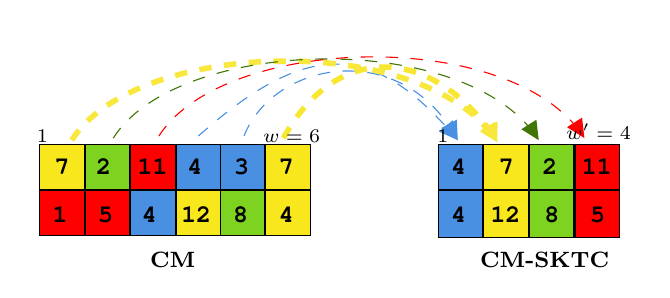
\begin{tikzpicture}[x=0.75pt,y=0.75pt,yscale=-1,xscale=1]
%uncomment if require: \path (0,300); %set diagram left start at 0, and has height of 300

%Shape: Rectangle [id:dp9120519996767289] 
\draw  [fill={rgb, 255:red, 248; green, 231; blue, 28 }  ,fill opacity=1 ] (39,134) -- (60.5,134) -- (60.5,156) -- (39,156) -- cycle ;
%Shape: Rectangle [id:dp5578762422129069] 
\draw  [fill={rgb, 255:red, 126; green, 211; blue, 33 }  ,fill opacity=1 ] (61,134) -- (82.5,134) -- (82.5,156) -- (61,156) -- cycle ;
%Shape: Rectangle [id:dp5149322189764962] 
\draw  [fill={rgb, 255:red, 255; green, 0; blue, 0 }  ,fill opacity=1 ] (83,134) -- (104.5,134) -- (104.5,156) -- (83,156) -- cycle ;
%Shape: Rectangle [id:dp8371364169912505] 
\draw  [fill={rgb, 255:red, 74; green, 144; blue, 226 }  ,fill opacity=1 ] (105,134) -- (126.5,134) -- (126.5,156) -- (105,156) -- cycle ;
%Shape: Rectangle [id:dp8774137890100953] 
\draw  [fill={rgb, 255:red, 74; green, 144; blue, 226 }  ,fill opacity=1 ] (126,134) -- (147.5,134) -- (147.5,156) -- (126,156) -- cycle ;
%Shape: Rectangle [id:dp8260064759507215] 
\draw  [fill={rgb, 255:red, 248; green, 231; blue, 28 }  ,fill opacity=1 ] (148,134) -- (169.5,134) -- (169.5,156) -- (148,156) -- cycle ;
%Shape: Rectangle [id:dp13750697143490287] 
\draw  [fill={rgb, 255:red, 255; green, 0; blue, 0 }  ,fill opacity=1 ] (39,156) -- (60.5,156) -- (60.5,178) -- (39,178) -- cycle ;
%Shape: Rectangle [id:dp12750267479029076] 
\draw  [fill={rgb, 255:red, 255; green, 0; blue, 0 }  ,fill opacity=1 ] (61,156) -- (82.5,156) -- (82.5,178) -- (61,178) -- cycle ;
%Shape: Rectangle [id:dp9453531436538745] 
\draw  [fill={rgb, 255:red, 74; green, 144; blue, 226 }  ,fill opacity=1 ] (83,156) -- (104.5,156) -- (104.5,178) -- (83,178) -- cycle ;
%Shape: Rectangle [id:dp019183616299335293] 
\draw  [fill={rgb, 255:red, 248; green, 231; blue, 28 }  ,fill opacity=1 ] (105,156) -- (126.5,156) -- (126.5,178) -- (105,178) -- cycle ;
%Shape: Rectangle [id:dp9174572360745898] 
\draw  [fill={rgb, 255:red, 126; green, 211; blue, 33 }  ,fill opacity=1 ] (126,156) -- (147.5,156) -- (147.5,178) -- (126,178) -- cycle ;
%Shape: Rectangle [id:dp2814590512908379] 
\draw  [fill={rgb, 255:red, 248; green, 231; blue, 28 }  ,fill opacity=1 ] (148,156) -- (169.5,156) -- (169.5,178) -- (148,178) -- cycle ;
%Shape: Rectangle [id:dp3867673825425666] 
\draw  [fill={rgb, 255:red, 74; green, 144; blue, 226 }  ,fill opacity=1 ] (231,134) -- (252.5,134) -- (252.5,157) -- (231,157) -- cycle ;
%Shape: Rectangle [id:dp45900611803416114] 
\draw  [fill={rgb, 255:red, 248; green, 231; blue, 28 }  ,fill opacity=1 ] (253,134) -- (274.5,134) -- (274.5,157) -- (253,157) -- cycle ;
%Shape: Rectangle [id:dp14536752724329527] 
\draw  [fill={rgb, 255:red, 126; green, 211; blue, 33 }  ,fill opacity=1 ] (275,134) -- (296.5,134) -- (296.5,157) -- (275,157) -- cycle ;
%Shape: Rectangle [id:dp7559601744598143] 
\draw  [fill={rgb, 255:red, 255; green, 0; blue, 0 }  ,fill opacity=1 ] (297,134) -- (318.5,134) -- (318.5,157) -- (297,157) -- cycle ;
%Shape: Rectangle [id:dp5499444494363386] 
\draw  [fill={rgb, 255:red, 74; green, 144; blue, 226 }  ,fill opacity=1 ] (231,156) -- (252.5,156) -- (252.5,179) -- (231,179) -- cycle ;
%Shape: Rectangle [id:dp6548836133040838] 
\draw  [fill={rgb, 255:red, 248; green, 231; blue, 28 }  ,fill opacity=1 ] (253,156) -- (274.5,156) -- (274.5,179) -- (253,179) -- cycle ;
%Shape: Rectangle [id:dp5995721454141998] 
\draw  [fill={rgb, 255:red, 126; green, 211; blue, 33 }  ,fill opacity=1 ] (275,156) -- (296.5,156) -- (296.5,179) -- (275,179) -- cycle ;
%Shape: Rectangle [id:dp8157813465457489] 
\draw  [fill={rgb, 255:red, 255; green, 0; blue, 0 }  ,fill opacity=1 ] (297,156) -- (318.5,156) -- (318.5,179) -- (297,179) -- cycle ;
%Curve Lines [id:da7793812944008702] 
\draw [color={rgb, 255:red, 74; green, 144; blue, 226 }  ,draw opacity=1 ] [dash pattern={on 4.5pt off 4.5pt}]  (115.5,130) .. controls (166.72,84.69) and (198.54,83.04) .. (238.66,129.83) ;
\draw [shift={(240.5,132)}, rotate = 230.07999999999998] [fill={rgb, 255:red, 74; green, 144; blue, 226 }  ,fill opacity=1 ][line width=0.08]  [draw opacity=0] (8.93,-4.29) -- (0,0) -- (8.93,4.29) -- cycle    ;
%Curve Lines [id:da17576300112648635] 
\draw [color={rgb, 255:red, 74; green, 144; blue, 226 }  ,draw opacity=1 ] [dash pattern={on 4.5pt off 4.5pt}]  (137.5,130) .. controls (151.29,94.54) and (211.65,82.37) .. (239.26,129.79) ;
\draw [shift={(240.5,132)}, rotate = 241.63] [fill={rgb, 255:red, 74; green, 144; blue, 226 }  ,fill opacity=1 ][line width=0.08]  [draw opacity=0] (8.93,-4.29) -- (0,0) -- (8.93,4.29) -- cycle    ;
%Curve Lines [id:da12939079412155663] 
\draw [color={rgb, 255:red, 248; green, 231; blue, 50 }  ,draw opacity=2 ] [dash pattern={on 4.5pt off 4.5pt}][line width=2]  (156.5,131) .. controls (181.25,85.65) and (226.58,85.07) .. (258.54,130.92) ;
\draw [shift={(259.5,133)}, rotate = 245.43] [fill={rgb, 255:red, 248; green, 231; blue, 60 }  ,fill opacity=1 ][line width=0.5]  [draw opacity=0] (8.93,-4.29) -- (0,0) -- (8.93,4.29) -- cycle    ;
%Curve Lines [id:da23437502293589474] 
\draw [color={rgb, 255:red, 248; green, 231; blue, 60 }  ,draw opacity=1, line width=0.5 ] [dash pattern={on 4.5pt off 4.5pt}][line width=2]  (54.5,132) .. controls (85.04,83.73) and (221.32,79.13) .. (257.9,130.61) ;
\draw [shift={(259.5,133)}, rotate = 237.8] [fill={rgb, 255:red, 248; green, 231; blue, 60 }  ,fill opacity=1 ][line width=0.5]  [draw opacity=0] (8.93,-4.29) -- (0,0) -- (8.93,4.29) -- cycle    ;
%Curve Lines [id:da16470429934928688] 
\draw [color={rgb, 255:red, 65; green, 117; blue, 5 }  ,draw opacity=1 ] [dash pattern={on 4.5pt off 4.5pt}]  (74.5,131) .. controls (105.04,82.73) and (241.32,78.13) .. (277.9,129.61) ;
\draw [shift={(279.5,132)}, rotate = 237.8] [fill={rgb, 255:red, 65; green, 117; blue, 5 }  ,fill opacity=1 ][line width=0.08]  [draw opacity=0] (8.93,-4.29) -- (0,0) -- (8.93,4.29) -- cycle    ;
%Curve Lines [id:da3875594417212562] 
\draw [color={rgb, 255:red, 255; green, 0; blue, 0 }  ,draw opacity=1 ] [dash pattern={on 4.5pt off 4.5pt}]  (96.5,130) .. controls (124.04,86.47) and (237.6,78.45) .. (286.45,115.07) .. controls (291.73,119.02) and (296.25,123.5) .. (299.83,128.51) ;
\draw [shift={(301.5,131)}, rotate = 237.8] [fill={rgb, 255:red, 255; green, 0; blue, 0 }  ,fill opacity=1 ][line width=0.08]  [draw opacity=0] (8.93,-4.29) -- (0,0) -- (8.93,4.29) -- cycle    ;

% Text Node
\draw (44,163) node [anchor=north west][inner sep=0.75pt]  [font=\large,color={rgb, 255:red, 0; green, 0; blue, 0 }  ,opacity=1 ] [align=left] {{\fontfamily{pcr}\selectfont \textbf{{\small 1}}}};
% Text Node
\draw (66,163) node [anchor=north west][inner sep=0.75pt]  [font=\large,color={rgb, 255:red, 0; green, 0; blue, 0 }  ,opacity=1 ] [align=left] {{\fontfamily{pcr}\selectfont {\small \textbf{5}}}};
% Text Node
\draw (87,163) node [anchor=north west][inner sep=0.75pt]  [font=\large,color={rgb, 255:red, 0; green, 0; blue, 0 }  ,opacity=1 ] [align=left] {{\fontfamily{pcr}\selectfont {\small \textbf{4}}}};
% Text Node
\draw (106,163) node [anchor=north west][inner sep=0.75pt]  [font=\large,color={rgb, 255:red, 0; green, 0; blue, 0 }  ,opacity=1 ] [align=left] {{\fontfamily{pcr}\selectfont {\small \textbf{12}}}};
% Text Node
\draw (131,163) node [anchor=north west][inner sep=0.75pt]  [font=\large,color={rgb, 255:red, 0; green, 0; blue, 0 }  ,opacity=1 ] [align=left] {{\fontfamily{pcr}\selectfont {\small \textbf{8}}}};
% Text Node
\draw (153,163) node [anchor=north west][inner sep=0.75pt]  [font=\large,color={rgb, 255:red, 0; green, 0; blue, 0 }  ,opacity=1 ] [align=left] {{\fontfamily{pcr}\selectfont {\small \textbf{4}}}};
% Text Node
\draw (236,163) node [anchor=north west][inner sep=0.75pt]  [font=\large,color={rgb, 255:red, 0; green, 0; blue, 0 }  ,opacity=1 ] [align=left] {{\fontfamily{pcr}\selectfont {\small \textbf{4}}}};
% Text Node
\draw (255,163) node [anchor=north west][inner sep=0.75pt]  [font=\large,color={rgb, 255:red, 0; green, 0; blue, 0 }  ,opacity=1 ] [align=left] {{\fontfamily{pcr}\selectfont {\small \textbf{12}}}};
% Text Node
\draw (281,163) node [anchor=north west][inner sep=0.75pt]  [font=\large,color={rgb, 255:red, 0; green, 0; blue, 0 }  ,opacity=1 ] [align=left] {{\fontfamily{pcr}\selectfont {\small \textbf{8}}}};
% Text Node
\draw (303,163) node [anchor=north west][inner sep=0.75pt]  [font=\large,color={rgb, 255:red, 0; green, 0; blue, 0 }  ,opacity=1 ] [align=left] {{\fontfamily{pcr}\selectfont {\small \textbf{5}}}};
% Text Node
\draw (45,140) node [anchor=north west][inner sep=0.75pt]  [font=\large,color={rgb, 255:red, 0; green, 0; blue, 0 }  ,opacity=1 ] [align=left] {{\fontfamily{pcr}\selectfont \textbf{{\small 7}}}};
% Text Node
\draw (153,140) node [anchor=north west][inner sep=0.75pt]  [font=\large,color={rgb, 255:red, 0; green, 0; blue, 0 }  ,opacity=1 ] [align=left] {{\fontfamily{pcr}\selectfont \textbf{{\small 7}}}};
% Text Node
\draw (65,140) node [anchor=north west][inner sep=0.75pt]  [font=\large,color={rgb, 255:red, 0; green, 0; blue, 0 }  ,opacity=1 ] [align=left] {{\fontfamily{pcr}\selectfont \textbf{{\small 2}}}};
% Text Node
\draw (85,140) node [anchor=north west][inner sep=0.75pt]  [font=\large,color={rgb, 255:red, 0; green, 0; blue, 0 }  ,opacity=1 ] [align=left] {{\fontfamily{pcr}\selectfont \textbf{{\small 11}}}};
% Text Node
\draw (131.5,140) node [anchor=north west][inner sep=0.75pt]  [font=\large,color={rgb, 255:red, 0; green, 0; blue, 0 }  ,opacity=1 ] [align=left] {{\fontfamily{pcr}\selectfont \textbf{{\small 3}}}};
% Text Node
\draw (109,140) node [anchor=north west][inner sep=0.75pt]  [font=\large,color={rgb, 255:red, 0; green, 0; blue, 0 }  ,opacity=1 ] [align=left] {{\fontfamily{pcr}\selectfont \textbf{{\small 4}}}};
% Text Node
\draw (280,140) node [anchor=north west][inner sep=0.75pt]  [font=\large,color={rgb, 255:red, 0; green, 0; blue, 0 }  ,opacity=1 ] [align=left] {{\fontfamily{pcr}\selectfont \textbf{{\small 2}}}};
% Text Node
\draw (236,140) node [anchor=north west][inner sep=0.75pt]  [font=\large,color={rgb, 255:red, 0; green, 0; blue, 0 }  ,opacity=1 ] [align=left] {{\fontfamily{pcr}\selectfont \textbf{{\small 4}}}};
% Text Node
\draw (299,140) node [anchor=north west][inner sep=0.75pt]  [font=\large,color={rgb, 255:red, 0; green, 0; blue, 0 }  ,opacity=1 ] [align=left] {{\fontfamily{pcr}\selectfont \textbf{{\small 11}}}};
% Text Node
\draw (259,140) node [anchor=north west][inner sep=0.75pt]  [font=\large,color={rgb, 255:red, 0; green, 0; blue, 0 }  ,opacity=1 ] [align=left] {{\fontfamily{pcr}\selectfont \textbf{{\small 7}}}};

\draw (91,185) node [anchor=north west][inner sep=0.75pt]   [align=left] {\textbf{{\footnotesize CM}}};
\draw (250,185) node [anchor=north west][inner sep=0.75pt]   [align=left] {\textbf{{\footnotesize CM-SKTC}}};

\node[text width=0.5cm, anchor=west, right] at (33,130) {\scriptsize $1$};
\node[text width=0.85cm, anchor=west, right] at (142,130) {\scriptsize $w=6$};
\node[text width=0.5cm, anchor=west, right] at (226,130) {\scriptsize $1$};
\node[text width=0.85cm, anchor=west, right] at (288,128) {\scriptsize $w'=4$};

%\node[text width=0.5cm, anchor=west, right] at (1.31,1.90) {\scriptsize $1$};
%\node[text width=0.5cm, anchor=west, right] at (1.25,0.32) {\scriptsize $d$};
\end{tikzpicture}

    \caption{An example for Count-Min sketch (CM) (left side) compression with CM-SKTC (right side). In this example, a CM of size $d=2, w=6$ is compressed into a CM-SKTC of size  $d=2, w'=4$. Values of the hash functions $g_1, g_2$ are represented by various colors. In row $i$, multiple counters with the same hash value of $g_i$ are represented by their maximum.}
    \label{sktc-fig:cm-sktc-example}
\end{figure}

\begin{algorithm}[htb]
    \small
    \begin{algorithmic}[1]
    \Statex vars:
    \Statex $h_1,\dots h_d$ - hash functions from flows to $[1,w]$
    \Statex $g_1, \dots g_d$ - hash functions from $[1,w]$ to $[1,w']$
        \Procedure{query}{$S^c, f$}
            \State $est \gets 0$
            \For{$j \in [1 \dots d]$}
        \If{$est > S^c[j][g_j\left(h_j(f)\right)]$}
        \State $est \gets S^c[j][g_j\left(h_j(f)\right)]$
        \EndIf
      \EndFor
      \State \Return $est$
        \EndProcedure

    \end{algorithmic}
    \caption{CM-SKTC estimation query}
    \label{sktc-alg:w-compression-query}
\end{algorithm}

% \begin{algorithm}[t!]
% \begin{algorithmic}[1]
% 		\REQUIRE{A compressed CM-SKTC $\textsl{S}^c$ (size $d \times w'$), a flow $f$}
% 		\ENSURE{An estimation of $f$}
% 		\RETURN $\min\limits_{j \in [1\dots d]} \left\{\textsl{S}^c[j][g_j\left(h_j(f)\right)]\right\}$
% \end{algorithmic}
% \caption{CM-SKTC estimation query}\label{sktc-alg:w-compression-query}
% \end{algorithm}


Yang et al.~\cite{yang2018elastic} present error bounds for compressing the CM when reducing $w$ to some divider $w'$ (i.e., $w=z\cdot w'$ for an integer $z$). The number of counters compressed to the same counter is fixed as $w / w'$. Our CM-SKTC, however, maps a variable number of counters to each counter using hashing. This number can vary among the counters in an array or among the arrays, thereby adding a taste of randomness. \inblue{Recall that in the CM sketch $\delta$ (the error probability) is a function of the number of columns and $\epsilon$ (the error) is a function of the number of rows. Our compression scheme reduces the number of columns, therefore, intuitively, the probability of estimating the flow size with error at most $\epsilon$ is reduced by some factor. In practice, given a probability $\delta$, the CM-SKTC is initialized with enough columns so that after compression the probability of estimating the flow size with at most error $\epsilon$ is greater than $1-\delta$. } \inred{Given a CM sketch with $d$ rows, and $w$ columns, and a compression ratio $w'/w$, Lemma~\ref{sktc-lmma:single-array-compression} presents the guarantees of the compressed sketch.}

\begin{lemma}
Given a CM $\textsl{S}$ with $d$ rows and $w$ columns, for appropriate parameters $(\epsilon, \delta')$, and a CM-SKTC  compression ratio $\frac{w'}{w} < 1$.
Let $N$ be the size of the stream and denote by  $\hat{f_i}$ the estimation of flow with size $f_i$.  
Denote by $\beta$ the term $$ \left(1-\left(1-\frac{1}{\epsilon w}\right)\left(1-\frac{N}{w(f_i+\epsilon N)}\right)^{\frac{w}{w'}-1+\sqrt{-2\ln(1-\delta)\frac{w}{w'}}}\right)^d.$$
The estimation $\hat{f}$ of flow $f$ satisfies 
$\hat{f} \leq f + \epsilon N$ with probability $1 - \beta -\delta'(1-\beta)$.
\label{sktc-lmma:single-array-compression}
\end{lemma}


\begin{proof}[\textbf{Proof of Lemma \ref{sktc-lmma:single-array-compression}}]
Following the compression, each counter in array $j \in [1,d]$ of \textsl{S}$^c$ is the maximum of all values of counters from \textsl{S}  mapped to this counter by the corresponding function from $g_j$. Since the $d$ arrays in \textsl{S}$^c$ are independent, we begin by analyzing each array error contribution by itself.
For some array, let denote by $X_l$ the number of cells that mapped to cell $l \in [1,w']$ in \textsl{S}$^c$. \inblue{As the hash functions map the domain $\{1,2,\dots, w\}$ uniformly to the range $\{1,2,\dots, w'\}$, $X_l$ is \inred{a random variable drawn from} a binomial distribution with $p = 1/w'$ and $n=w$.}
As $X_l$ is binomial, $e \triangleq E(X_l) = \frac{w}{w'}$. \inblue{We now bound the number of rows in the original CM sketch that map to the rows in the compressed sketch using the Chernoff bound:} 
\begin{flalign*}
&\text{Pr}\left(X_l > e+\sqrt{-2\ln(\sqrt[d]{1-\delta})e}\right)\\
&= \text{Pr}\left(X_l > \left(1+\sqrt{
-2\ln(\sqrt[d]{1-\delta}) / e
}\right)e\right)  \\
\stackrel{\text{Chernoff bound}}{\leq} &e^{-
\frac{\left(
\sqrt{
-2\ln(\sqrt[d]{1-\delta}) / e
}\right)^2r}
{2}}= e^{-\frac{-2\ln(\sqrt[d]{1-\delta})e}{2e}} \\
&= e^{\ln(\sqrt[d]{1-\delta})} = \sqrt[d]{1-\delta}.
\end{flalign*}
Let  $C = \left\lceil e+\sqrt{-2\ln(1-\sqrt[d]{1-\delta})e} \right\rceil$. Following the compression, each counter in \textsl{S}$^c$ is the maximum value of at least $C$  counters from \textsl{S} \inblue{with probability at most $\sqrt[d]{1-\delta}$}. 

We bound the error for a flow $f_i$, which is mapped to one counter in \textsl{S} and compressed with at most $C-1$ other counters to a new counter \inblue{with probability at least $1-\sqrt[d]{1-\delta}$}. Denote by $n_1,...,n_C$ the number of packets which do not belong to flow $f_i$, but are mapped to the $C$ counters mapped to counter \textsl{S}. From the CM sketch, $\text{C}(n_i) \leq \frac{N}{w}$ for every $n_i$.
Without loss of generality assume that $f_i$ is mapped to $n_1$. Conclude that the estimation $\hat{f}_i$ is 
%\begin{flalign*}
$\hat{f}_i = \max(n_1+f_i,n_2,...,n_C)$ and accordingly
% \begin{flalign*}
% \text{Pr}(\hat{f}_i \geq f_i + \epsilon N)\\ 
% =\text{Pr}(\max(n_1+a_i,n_2,\dots,n_C) \geq f_i + \epsilon N)  \\ 
% \leq 1 - \text{Pr}(\max(n_1+a_i,n_2,\dots,n_C) < f_i + \epsilon N)  \\ 
% =1 - \text{Pr}(n_1+f_i < f_i + \epsilon N)\cdot \prod\limits_{j=2}^C \text{Pr}(n_j < f_i + \epsilon N)  \\
% %\end{align*}
% %\begin{align*}
% = 1 - \text{Pr}(n_1 < \epsilon N) \cdot \prod\limits_{j=2}^C \text{Pr}(n_j < f_i + \epsilon N) \\
%  \stackrel{\text{Markov inequality}}{\leq} 1 - \left(1-\frac{E(n_1)}{\epsilon N}\right) \cdot \prod\limits_{j=2}^C \left(1-\frac{E(n_j)}{f_i + \epsilon N}\right) \\
% \leq  1- \left(1-\frac{1}{w\epsilon}\right)\left(1-\frac{N}{w(f_i+\epsilon N)}\right)^{C-1}
% \end{flalign*}
\begin{gather*}
\text{Pr}(\hat{f}_i \geq f_i + \epsilon N)\\ 
=\text{Pr}(\max(n_1+a_i,n_2,\dots,n_C) \geq f_i + \epsilon N)  \\ 
\leq 1 - \text{Pr}(\max(n_1+a_i,n_2,\dots,n_C) < f_i + \epsilon N)  \\ 
=1 - \text{Pr}(n_1+f_i < f_i + \epsilon N)\cdot \prod\limits_{j=2}^C \text{Pr}(n_j < f_i + \epsilon N) \\
%\end{align*}
%\begin{align*}
= 1 - \text{Pr}(n_1 < \epsilon N) \cdot \prod\limits_{j=2}^C \text{Pr}(n_j < f_i + \epsilon N)
\end{gather*}
\begin{gather*}
 \stackrel{\text{Markov inequality}}{\leq} 1 - \left(1-\frac{E(n_1)}{\epsilon N}\right) \cdot \prod\limits_{j=2}^C \left(1-\frac{E(n_j)}{f_i + \epsilon N}\right) \\
\leq  1- \left(1-\frac{1}{w\epsilon}\right)\left(1-\frac{N}{w(f_i+\epsilon N)}\right)^{C-1}
\end{gather*}

\inblue{As the hash functions are pairwise independent, we can use this bound to bound the error of $\hat{f}_i$, the estimation of flow $f_i$. By definition $\hat{f}_i = \min(\hat{f}_i^1,\hat{f}_i^2,\dots,\hat{f}_i^d)$.}

\begin{flalign*}
&\text{Pr}(\hat{f}_i \geq f_i + \epsilon N) = \text{Pr}(\min(\hat{f}_i^1,\dots,\hat{f}_i^d) \geq f_i + \epsilon N) \\
&\leq \prod\limits_{j=1}^d \text{Pr}(\hat{f}_i^j \geq f_i + \epsilon N)
\end{flalign*}

We have shown that for any $j$: $\text{Pr}(\hat{f}_i^j \geq f_i + \epsilon N) \leq 1- \left(1-\frac{1}{w\epsilon}\right)\left(1-\frac{N}{w(f_i+\epsilon N)}\right)^{C-1}$, with probability $\delta' = \sqrt[d]{1-\delta}$. Therefore, \inblue{as the hash functions as pair-wise independent,} we can conclude that the following holds with probability of $\sqrt[d]{1-\delta}^d = 1-\delta$:
\begin{flalign*}
&\text{Pr}(\hat{f}_i \geq f_i + \epsilon N) \leq \prod\limits_{j=1}^d \text{Pr}(\hat{f}_i^j \geq f_i + \epsilon N)\\
&\leq \prod\limits_{j=1}^d 1- \left(1-\frac{1}{w\epsilon}\right)\left(1-\frac{N}{w(f_i+\epsilon N)}\right)^{C-1} \\
&= \left(1- \left(1-\frac{1}{w\epsilon}\right)\left(1-\frac{N}{w(f_i+\epsilon N)}\right)^{C-1}\right)^d = \beta. 
\end{flalign*}

With probability of $1-\delta$ the following holds: $\text{Pr}(\hat{f}_i \geq f_i + \epsilon N) \leq \beta$ , thus $\text{Pr}(\hat{f}_i \leq f_i + \epsilon N) \geq 1-\beta$ with probability \inblue{at least} $1-\delta$. Therefore the probability that $\hat{f}_i \leq f_i + \epsilon N$ is at least $(1-\delta)(1-\beta)=1-\beta-\delta(1-\beta)$.  
\end{proof}


\inblue{Lemma~\ref{sktc-lmma:single-array-compression} shows that \inred{compressing a sketch with parameter $\delta$ yields a sketch with parameter $\beta + \delta(1-\beta)$, where $\beta$ is as defined in the lemma. It follows that to achieve probability $\delta$ \textbf{after} compression, we must instantiate the uncompressed sketch with parameter $(\delta - \beta) / (1 - \beta)$.}
 Denote $\delta' = \beta + \delta(1-\beta)$. We empirically analyze how the compression affects the probability. Table~\ref{sktc-tbl:delta_tah} shows how $\delta'$ is affected by changes in $\delta$, $w' / w$, and $\epsilon$ respectively. $\delta'$ remains less than $3\delta$, therefore we initialize the CM sketch to have the number of columns for $3\delta$ as opposed to $\delta$. As the number of columns is $\lceil\ln 1/\delta \rceil$, generally, we need to add a single column in order for the error probability after compression to be less than $\delta$.}

\begin{table}[b]
\inblue{
\caption{\inred{Error probabilities after compression, for values of $\delta$, $\epsilon$  and the resize factor, as defined by Lemma~\ref{sktc-lmma:single-array-compression}.}}
    \label{sktc-tbl:delta_tah}
    \begin{tabular}{|c|c|c|c|c|}
        \cline{2-5} 
        \multicolumn{1}{c}{Resize Factor} & \multicolumn{2}{|c|}{ $0.6$} & \multicolumn{2}{c|}{ $0.9$}\tabularnewline
        \cline{2-5} 
        \multicolumn{1}{c}{$\delta \quad \backslash \quad \epsilon$} & \multicolumn{1}{|c|}{ $\quad\; 0.02 \quad\;$} & \multicolumn{1}{c|}{$\quad\; 0.06 \quad\;$} & \multicolumn{1}{c|}{$\quad\; 0.02  \quad\;$} & \multicolumn{1}{c|}{$\quad\; 0.06 \quad\;$}\tabularnewline
        \hline
        $0.04$ & $0.0936$  & $0.1177$  & $0.0841$  & $0.0925$\tabularnewline
        \hline 
        $0.08$ & $0.1791$  & $0.217$  & $0.1648$ & $0.1808$\tabularnewline
        \hline
    \end{tabular}
}
\end{table}


%\begin{figure}
%    \centering
%    \includegraphics[width=0.9\columnwidth]{figures/new_delta.png}
%    \caption{$\delta'$ as a function of $\delta$.}
%    \label{sktc-fig:new_delta}
%\end{figure}

%\begin{figure}
%    \centering
%    \includegraphics[width=0.9\columnwidth]{figures/new_resize_factor.png}
%    \caption{$\delta'$ as a function of the resize factor.}
%    \label{sktc-fig:new_resize_factor}
%\end{figure}

%\begin{figure}
%    \centering
%    \includegraphics[width=0.9\columnwidth]{figures/new_epsilon.png}
%    \caption{$\delta'$ as a function of $\epsilon$.}
%    \label{sktc-fig:new_epsilon}
%\end{figure}

\section{The Traffic-Aware CM}\label{sktc-sec:resize}
The system measures a stream of data that is split in a distributed fashion across several ingestion nodes. 
Upon stream ingestion completion, the nodes communicate with a centralized server which can then answer queries. This is depicted in Figure~\ref{sktc-fig:ingestion-nodes}. 
Queries are agnostic to the specific architecture, namely, they only refer to the complete stream as a whole and do not refer to its parts observed by each of the nodes. 
%Assume that the channel between the nodes to the centralized server has limited bandwidth. 
There is a clear tradeoff between the summaries size sent to the server and its ability to answer queries accurately.  
Accordingly, we would like to optimally use compression to allow high accuracy.  The \textbf{MM}~\cite{yang2018elastic} scheme was proposed to reduce summary size through compression of CMs maintained by the nodes but the fact it can be compressed in only particular ratios restricts it from taking advantage of all bandwidth to the server. 
%In a similar fashion to \cite{yang2018elastic}, we would like to efficiently utilize the available bandwidth for a given accuracy. Therefore, we present a trade-off between the accuracy required and the overall amount of data sent over the network. Specifically, we aim to reduce the overall amount of data sent over the network for given accuracy bounds. To this end, we aim to use sketch compression to reduce the amount of data sent but maintain a sufficiently low error bound. 
%In \cite{yang2018elastic}, the authors build a CM $\textsl{S}$ for counting mouse flows occurrences, and before data transfer to the centralized server, their method compressed the CM by joining multiple cell values into one cell. A clear drawback of the Zip-sketch is that it can only compress the original sketch to a limited set of compression sizes, which are the dividers of the original Count-Min sketch size.

%We assume streams are ingested in a distributed fashion across several ingestion nodes. Upon stream ingestion completion, the nodes communicate with a centralized server, which can then answer queries. This is depicted in Figure~\ref{sktc-fig:ingestion-nodes}. In a similar fashion to \cite{yang2018elastic}, we would like to efficiently utilize the available bandwidth for a given accuracy. The queries are agnostic to the specific architecture, they do not know how many ingestion nodes were used if at all, all they require is a promise on the accuracy of the query result. Therefore, we present a trade-off between the accuracy required and the overall amount of data sent over the network. Specifically, we aim to reduce the overall amount of data sent over the network for given accuracy bounds. To this end, we aim to use sketch compression to reduce the amount of data sent but maintain a sufficiently low error bound. In \cite{yang2018elastic}, the authors build a CM $\textsl{S}$ for counting mouse flows occurrences, and before data transfer to the centralized server, their method compressed the CM by joining multiple cell values into one cell. A clear drawback of the Zip-sketch is that it can only compress the original sketch to a limited set of compression sizes, which are the dividers of the original Count-Min sketch size.

In network traffic, flow size distribution among switches can be imbalanced~\cite{Niagara, Sadeh19}.  For instance, the location of nodes along paths of various lengths or employment of particular network functions in the nodes can result in nodes receiving a small portion of the network stream while others more traffic.
We leverage this skew to reduce the summaries size sent to the server. Specifically, we aim to compress the sketches sent by ingestion nodes that received a small portion of the overall stream more than those sketches of nodes with higher portions of traffic. We say that a sketch   compression from $w$ columns to $w'$ columns has a \emph{compression ratio} of $w'/w$. 
As mentioned, the number of rows is not reduced. 



The design of Traffic-Aware Count-Min Sketch (TA-CM) is as follows: Given parameters $(\epsilon,\delta)$, where $\epsilon$ is the desired error, $\delta$ is the maximum error probability, we instantiate a CM on every ingestion node with parameters $(\sigma \cdot \epsilon, \delta)$ for some $0 < \sigma \leq 1$. $\frac{1}{\sigma}$ is an enlargement factor and is known in advance to the ingestion nodes and the centralized server. We increase the size of the sketch at the ingestion nodes by $\frac{1}{\sigma}$ and as such decrease their respective error (as the error is tied to the number of columns). By enlarging the sketches at the ingestion nodes, we can compress them while maintaining an error within the desired bounds. When the ingestion period ends, the following protocol takes place:
%\begin{enumerate}

\emph{(i)} Each ingestion node reports to the central node its local stream size.

\emph{(ii)} The centralized server computes each ingestion node's compression ratio.

\emph{(iii)} Every ingestion node compresses its CM with the CM-SKTC method, then sends its summary to the centralized server.

\emph{(iv)} The centralized node can query a single flow $f_j$ by querying every CM-SKTC separately and summing up the results to calculate the estimation for flow $f_j$.
%\end{enumerate}

To achieve an overall maximum error of $\epsilon$ for an arbitrary flow size estimation, the centralized server can (naively) request a compression ratio of $1 / \sigma$. Theorem \ref{sktc-thm:two-sketches} shows that when there are two ingestion nodes, there are optimal compression ratios that minimize the total summaries size while maintaining the error bounds of the flow size estimation in the centralized server to be at most $\epsilon$.

Intuitively, the proof is based on constraints that: (i) the overall error be within the desired bounds, and (ii) the size of sent traffic be smaller than the naive solution (i.e., less than $2\cdot w \cdot d$ where $w \cdot d$ is the size of a CM with parameters $(\epsilon, \delta)$).

\begin{theorem}
For given Count-Min sketch parameters $\epsilon, \delta$,  initial resize factor $\sigma$, and two CMs $\textsl{S}_1$, $\textsl{S}_2$, with stream sizes of $N_1$, $N_2$ respectively, such that w.l.o.g $N_1 \geq N_2$. The TA-CM resize factors $r_1=\frac{k + 1}{\sigma  (k + \sqrt{k})}$ and $r_2=\frac{k+1}{\sigma(\sqrt{k}+1)}$ for $k = N_1 / N_2$ generate the minimal amount of network communication such that the error is bounded by $\epsilon$ \inblue{ with probability at least $1-(\beta + \delta (1-\beta))$}.
\label{sktc-thm:two-sketches}
\end{theorem}

\begin{proof}[\textbf{Proof of Theorem \ref{sktc-thm:two-sketches}}]
Denote by $f$ the flow whose size is being estimated and by $\hat{f}$ the estimation. Given a CM with parameters $(\sigma \epsilon, \delta)$, after compression by a factor of $r$, the following inequality holds \inblue{with probability at least $1-(\beta + \delta (1-\beta))$}, by Lemma~\ref{sktc-lmma:single-array-compression}:
$ f \leq \hat{f} \leq f + \sigma \epsilon r N$
\noindent Denote $f_1$, $f_2$ the flow ingested by $\textsl{S}_1$, $\textsl{ S}_2$ respectively, and, likewise, their estimations (after compression) by $\hat{f_1}$, $\hat{f_2}$.

\inblue{
Recall that:
$f_1 \leq \hat{f}_1 \leq f_1 + \sigma \epsilon r_1 N_1$,
and 
$f_1 \leq \hat{f}_2 \leq f_2 + \sigma \epsilon r_2 N_2$,
where
$f = f_1 + f_2$.
}
Therefore, \inblue{due to the mergeability property}, the estimation by the central entity is:
\begin{align*}
    f \leq \hat{f_1} + \hat{f_2} \leq f + \sigma \epsilon (r_1 N_1 + r_2 N_2) \\
    f_1 + f_2 \leq \hat{f_1} + \hat{f_2} \leq f_1 + \sigma \epsilon r_1 N_1 + f_2 + \sigma \epsilon r_2 N_2
\end{align*}
\noindent Recall that we would like to maintain an overall error of $\epsilon$, therefore we require that:
\begin{align*}
    \sigma(r_1 N_1 + r_2 N_2) \leq N,
\end{align*}
\noindent and that $N_1 = k N_2$. Denote the ratio between $r_1$ and $r_2$ as $\alpha=r_1 / r_2$. As $N_1$ is larger than $N_2$, we expect $\alpha$ to be less than $1$, as the information retained in $\textsl{S}_2$ will have less of an impact than $\textsl{S}_1$:
\begin{align*}
   & N_1 + N_2 = N \Rightarrow  N_2 = \frac{N}{k+1} \\
    &\sigma(r_1 N_1 + r_2 N_2) = \sigma (\alpha k r_2 N_2 + r_2 N_2) \leq N \\
    &r_2 \leq \frac{k+1}{\sigma (\alpha k +1)}
\end{align*}

To reduce the total summaries size as much as possible, the ratios $r_1$ and $r_2$ should be as large as possible:
\begin{align}
    r_2 = \frac{k+1}{\sigma (\alpha k +1)}
    \label{sktc-eq:c2-size}
\end{align}

 The goal is to reduce the total summaries size in comparison to trivial resizing by a factor of $1/\sigma$. %Let $wd$ be the size of the CM prior to resizing, therefore 
 We require:
\begin{align}
%    &\frac{wd}{r_1} + \frac{wd}{r_2} \leq \frac{wd}{1 / \sigma} + \frac{wd}{1 / \sigma} \nonumber \\
    &\frac{1}{r_1} + \frac{1}{r_2} \leq 2 \cdot \frac{1}{1 / \sigma} = 2\sigma \label{sktc-eq:size-constracint}
\end{align}

\noindent To achieve minimum summaries size, we minimize the left-hand size of  Equation~(\ref{sktc-eq:size-constracint}). \inblue{Recall that $r_1 = \alpha r_2$ for some $\alpha \in (0, \infty)$.}
\begin{align*}
    &\min_{\alpha \in (0, \infty)} \left\{ \frac{1}{r_1} + \frac{1}{r_2} \right\} = \min_{\alpha \in (0, \infty)} \left\{ \frac{1}{\alpha r_2} + \frac{1}{r_2} \right\} = \\
%    &\min_{\alpha \in (0, \infty)} \left\{ \frac{\sigma (\alpha k +1)}{\alpha(k+1)} + \frac{\sigma (\alpha k +1)}{k+1} \right\} = \\
    &\min_{\alpha \in (0, \infty)} \left\{ \frac{1 + \alpha}{\alpha r_2}\right\} \stackrel{(i)}{=} \min_{\alpha \in (0, \infty)} \left\{ \sigma (\alpha k +1) \frac{1+ \alpha}{\alpha(k+1)} \right\} \stackrel{(ii)}{=} \\
    &\min_{\alpha \in (0, \infty)} \left\{ \alpha k + \frac{1}{\alpha} \right\}
\end{align*}
\noindent Where (i) is from Equation~(\ref{sktc-eq:c2-size}) and (ii) is by removing constants not affected by $\alpha$. The minimum is for $\alpha = 1 / \sqrt{k}$, implying $\alpha < 1$ for  $k > 1$, as expected. Finally, our last constraint is that merging the sketches by factors other than $1/\sigma$ should provide smaller summaries size:
\begin{align*}
    &\frac{1}{r_1} + \frac{1}{r_2} = \sigma (\alpha k + 1 ) \frac{1+\alpha}{\alpha (k+1)} \stackrel{\alpha = 1 / \sqrt{k}}{=} \sigma \frac{(\sqrt{k} + 1)^2}{k+1}.
    %\\
%    &\sigma \frac{(\sqrt{k} + 1)^2}{k+1} \stackrel{\text{easy to see}}{\leq} 2 \sigma \Rightarrow k \geq 1
\end{align*}
%\begin{align*}
%    &\frac{1}{r_1} + \frac{1}{r_2} = \sigma (\alpha k + 1 ) \frac{1+\alpha}{\alpha (k+1)} \stackrel{\alpha = 1 / \sqrt{k}}{=} \\
%    &\sigma \frac{(\sqrt{k} + 1)^2}{k+1} \stackrel{\text{easy to see}}{\leq} 2 \sigma \Rightarrow k \geq 1
%\end{align*}
\end{proof}

\inblue{The theorem shows that, as the imbalance in ingested stream parts between the nodes ($k$) increases, sketch $\textsl{S}_2$ is compressed to a higher degree. Furthermore, at the extreme case (i.e., $k = \infty$), $\textsl{S}_1$ is compressed by a factor of $1/ \sigma$, whereas $\textsl{S}_2$ is compressed by a factor of $\infty$. At this extremity, $\textsl{S}_2$ contains no information, thus this compression is intuitive. Furthermore, when $k=1$ both sketches are compressed by a ratio of $1 / \sigma$, which is also intuitive.
}

%As $k$ increases, the resize factor of $\textsl{S}_2$ increases. This is expected, as it has less of an impact on the answer to the query. Note that the summaries size with the optimal resize factors tends to half that of the summaries size sent in the trivial case, therefore utilizing optimal resizing upon uneven stream distribution leads to better usage of network bandwidth.


%So far we showed that in the case of two ingestion nodes we can resize the data in a way that maintains the error bounds within certain limits and decrease the traffic from ingestion nodes to the centralized server. However, in real networks, many ingestion nodes measure the traffic across the network. In the following Theorem, we expand the result of Theorem \ref{sktc-thm:two-sketches} to the general case of $n$ ingestion nodes.

We now generalize Theorem~\ref{sktc-thm:two-sketches} to the practical case of an arbitrary number of $n$ nodes.
We again maintain error bounds within certain limits.
\inblue{We first prove a helpful lemma:}
%\dor{We need to fit this Lemma into the text}
\begin{lemma}
For $n \geq 2$ the variables $1 \leq y_1,..,y_n$ satisfy 
\[\textstyle \frac{\left(1+\sum\limits_{i=1}^n \prod\limits_{j=i}^n \sqrt{y_j}\right)^2}{
\left(1+\sum\limits_{i=1}^n \prod\limits_{j=i}^n y_j\right)}
\leq n+1.\]
%\[\textstyle \dfrac{\left(1+\sum\limits_{i=1}^n \prod\limits_{j=i}^n \sqrt{x_j}\right)^2}{ 
%1+\sum\limits_{i=1}^n \prod\limits_{j=i}^n x_j}
%\leq n+1.\]
\label{sktc-lemma:sqrt-sums-lemma}
\end{lemma}
\begin{proof}[\textbf{Proof of Lemma \ref{sktc-lemma:sqrt-sums-lemma}}]
Let $y_1,\dots,y_n$ be as required.
\inblue{Denote:
\[x_i \triangleq \prod\limits_{j=i}^n y_j.\]
Note that, as $1 \leq y_1 \dots y_n$, then $1 \leq x_i$ for all $i$.}

As \[\left(1+\sum\limits_{i=1}^n \sqrt{x_i}\right)^2 = 1+\sum\limits_{i=1}^n x_i+\sum\limits_{i=1}^n 2\sqrt{x_i} + \sum\limits_{i\neq j} \sqrt{x_ix_j},\]
then
\[\frac{\left(1+\sum\limits_{i=1}^n \sqrt{x_i}\right)^2}{1+\sum\limits_{i=1}^n x_i} = 1+ \frac{\sum\limits_{i=1}^n 2\sqrt{x_i} + \sum\limits_{i\neq j} \sqrt{x_ix_j}}{1+\sum\limits_{i=1}^n x_i}\]
so we need to prove that
\[\frac{\sum\limits_{i=1}^n 2\sqrt{x_i} + \sum\limits_{i\neq j} \sqrt{x_ix_j}}{1+\sum\limits_{i=1}^n x_i} \leq n\]

\inblue{
Using the arithmetic-mean--geometric-mean inequality:
\[\sum\limits_{i\neq j} \sqrt{x_ix_j} \leq \sum\limits_{i\neq j} \frac{x_i + x_j}{2}=\sum\limits_{i=1}^n (n-1)x_i.\]
The divisor disappears as we double count every $x_i$: once on the left hand of the $+$ and once on the right hand.
Furthermore, for any $x_i \geq 1$:
\[2 \sqrt{x_i}+(n-1)x_i \leq 1 + n\cdot x_i.\]
Putting these together we get:
\[\sum\limits_{i=1}^n 2\sqrt{x_i} + \sum\limits_{i\neq j} \sqrt{x_ix_j} \leq \sum\limits_{i=1}^n 2\sqrt{x_i} + \sum\limits_{i=1}^n (n-1)x_i =\]
\[\sum\limits_{i=1}^n \left(2 \sqrt{x_i}+\left(n-1\right)x_i \right)\leq \sum\limits_{i=1}^n \left( 1 + n\cdot x_i\right)= n +n\sum\limits_{i=1}^n x_i \]
Finally:
\[\frac{\sum\limits_{i=1}^n 2\sqrt{x_i} + \sum\limits_{i\neq j} \sqrt{x_ix_j}}{1+\sum\limits_{i=1}^n x_i} \leq \frac{n +n\sum\limits_{i=1}^n x_i}{1 +\sum\limits_{i=1}^n x_i}=n\]
}
\end{proof}

We now use the lemma to prove the following theorem:
\begin{theorem}
Given $n \geq 2$ CMs $\textsl{S}_i$, with stream sizes $N_1 \ge N_2 \ldots \ge N_n$. Denote $k_i=N_i/N_{i+1}$ for $i \in [1,n-1]$ and $k_n = 1$.
%of $N_i$ for $i\in [1,n]$. Let $k_i=N_i/N_{i+1}$ and $k_n = 1$. If w.l.o.g $\forall i \in [1,n-1]: k_i \geq 1$
The optimal TA-CM resize factors are \[
\forall i \in [1,n-1]: \ r_i = \frac{\inblue{r_{i+1}}}{\sqrt{k_i}}
\quad  \text{and} \quad  
r_n = \frac{\sum\limits_{i=1}^n \prod\limits_{j=i}^n k_j}{\sigma(\sum\limits_{i=1}^n {\prod\limits_{j=i}^n \sqrt{k_j})}}.\]
\label{sktc-thm:n-sketches}
\end{theorem}

\begin{proof}[\textbf{Proof of Theorem \ref{sktc-thm:n-sketches}}]
The proof follows a similar path as the proof for Theorem~\ref{sktc-thm:two-sketches}. Denote by $f_i$ the size of the stream $i$ observed by $\textsl{S}_i$, and the estimations by $\hat{f_i}$. Denote by $r_i$ the compression ratio of $\textsl{S}_i$. \inblue{Let $\delta'$ be the probability calculated for some compression rate $r$, to be determined}. \inblue{Using the mergeability property, the estimation by the central entity, with probability at least $1-\delta'$}, is:
\[ f \leq \sum_i \hat{f_i} \leq f + \sigma \epsilon \sum_i r_i N_i \]
\[ \sum_i f_i \leq \sum_i \hat{f_i} \leq \sum_i \left(f_i + \sigma \epsilon r_i N_i\right) \]
Recall that we wish to maintain an overall bound of $\epsilon$, thus:
\[\sigma \epsilon \sum_i r_i N_i \leq \epsilon N\]

Denote $k_i = \frac{N_i}{N_{i+1}}$, and $\alpha_i=\frac{r_i}{r_{i+1}}$. Therefore:
\[\sigma \epsilon r_n N_n \sum\limits_{i=1}^{n} \prod\limits_{j=i}^n \alpha_j k_j  \leq \epsilon N \]
Since $N = N_1+N_2+...+N_n$ and $N_i = N_n \cdot \prod\limits_{j=i}^n k_j $, similar to the proof for Theorem~\ref{sktc-thm:two-sketches}, observe that
%\[ c_n \leq \frac{\sum\limits_{i=1}^{n} \prod\limits_{j=i}^n k_j}{\sigma\left(\sum\limits_{i=1}^{n} \prod\limits_{j=i}^n \alpha_j k_j\right)}\]
\[ r_n \leq \left(\sum\limits_{i=1}^{n} \prod\limits_{j=i}^n k_j\right) / \left(\sigma \cdot \sum\limits_{i=1}^{n} \prod\limits_{j=i}^n \alpha_j k_j\right).\]
We maximize $r_n$ to minimize summaries size. We choose minimal such $\alpha_i$ values by finding the minimum of 
%\[\min_{\alpha_i} \left\{\sum_{i=1}^n \frac{1}{c_i} \right\}\]
$\min_{\alpha_i} \left\{\sum_{i=1}^n \frac{1}{r_i} \right\}$. 


Following the proof for Theorem~\ref{sktc-thm:two-sketches} we use $\alpha_i = \frac{1}{\sqrt{k_i}}$ brings the summaries size to less than the trivial compression~\footnote{We also conjecture that it is a local minima.}.
Therefore, we reduce the size if the following holds:
\[  \left(1+\sum\limits_{i=1}^{n-1} \prod\limits_{j=i}^{n-1}\sqrt{k_j}\right)^2 / \left(1+\sum\limits_{i=1}^{n-1} \prod\limits_{j=i}^{n-1}k_j\right) \leq (n-1)+1\]
%\[  \frac{\left(1+\sum\limits_{i=1}^{n-1} \prod\limits_{j=i}^{n-1}\sqrt{k_j}\right)^2}{1+\sum\limits_{i=1}^{n-1} \prod\limits_{j=i}^{n-1}k_j} \leq n\]
By Lemma \ref{sktc-lemma:sqrt-sums-lemma} this expression is true for all ratios $k_i \geq 1$
and the resize factors are given by:
%\[ c_n = \frac{\sum\limits_{i=1}^n \prod\limits_{j=i}^n k_j}{\sigma(\sum\limits_{i=1}^n {\prod\limits_{j=i}^n \sqrt{k_j})}}\]
\[ r_n = \left(\sum\limits_{i=1}^n \prod\limits_{j=i}^n k_j\right) / \left(\sigma \cdot \sum\limits_{i=1}^n {\prod\limits_{j=i}^n \sqrt{k_j}}\right),\]
implying $r_i = \frac{r_{i+1}}{\sqrt{k_i}}$. Finally, using $r_n$ to calculate $\delta'$ (i.e., taking the lowest probability), we have proven our theorem.
\end{proof}

\inblue{
Theorem~\ref{sktc-thm:n-sketches} shows that sketches that have ingested a larger portion of the overall traffic are compressed less. This is similar to the case of $2$ nodes, as nodes that have ingested less traffic have a smaller impact on the query. Note that if all nodes ingest an equal part of the stream, i.e., $k_i=1$ for all $i$, then the compression ratio is $1/\sigma$ as expected.}

\section{The Traffic-Aware KMV for Cardinality Estimation}\label{sktc-sec:kmv-sktc}
We now present Traffic-Aware KMV (\emph{TA-KMV}), a method to compress the KMV sketch~\cite{giroire2009order, KMV}, \inred{a known tool for computing the number of distinct flows in a stream, also known as its cardinality}.  For the case of a single node KMV works as follows: For every flow $f_1,f_2,\dots$ it generates \inred{hash values} $h_1,h_2,\dots$ and it retains the $k$ smallest values - $\{h_1', h_2', \dots, h_k'\}$. The cardinality estimation the sketch calculates is $\frac{k}{\max\limits_{i \in [1,k]}\{h_i'\}}$. Errors can include \inred{overestimations} or underestimations of the cardinality and the relative standard error is $\frac{1}{\sqrt{k}}$. 


\inred{Also for this sketch we} refer to the scenario presented in Figure~\ref{sktc-fig:ingestion-nodes}, with nodes sending summaries to a centralized server through a channel with bounded bandwidth.  
As a simple baseline solution, every node can compute the hash values for all the flows it observes and send the $k$ minimal values among them to the centralized node. This results in a total number of $n \cdot k$ values sent over the network. \inred{Then, the central node simply orders
all the $n \cdot k$ values it receives for computing the value which is the $k$-th smallest in its size among them, denoted as $h'_k$. It estimates the cardinality of the complete stream as $\frac{k}{h'_k}$. Note that although not all observed values were shared by the various nodes, the value of $h'_k$ necessarily equals the $k$-th smallest hash value among all the values for the complete stream.}

\inred{
We aim to develop solution that reduces the total number of values that are sent for better utilizing the available bandwidth.} 

Our proposal for this distributed sketch is as follows: Given parameter $k$, we instantiate \emph{KMV sketch} on the ingestion nodes with parameter $k \ln{k}$. When the ingestion ends, the following communication takes place:

\emph{(i)} Ingestion nodes report their cardinality estimation size to the centralized server.

\emph{(ii)} The central server computes for each ingestion node $i$ its compression ratio $n_i$.

\emph{(iii)} Each ingestion node sends its $n_i$ minimal values to the centralized server.

We suggest a heuristic of calculating compression ratios $n_i$. We are unable to provide closed form error bounds for this heuristic. Instead, in Section~ \ref{sktc-sec:evaluation}, we show that this method performs well in realistic scenarios.

The goal is for the centralized server to receive some group of $k$ flow hashes such that the group has as large overlap as possible with the group of global $k$ minimal flow hashes. The method works as follows: Let $e_i$ be the cardinality estimation of server $i$. First, each ingestion node $i$ sends $e_i$ to the central server, and receives the total estimation $\sum\limits_{j=1}^n e_j$ in return. Each ingestion node $i$ can then compute the estimation ratio
$r_i = \frac{e_i}{\sum\limits_{j=1}^n e_j}$ and sends a summary of size  $s_i = r_i \cdot k \ln{k}$. In this case the total summaries size is: 
\[\sum\limits_{i=1}^n s_i = \sum\limits_{i=1}^n  r_i \cdot k \ln{k}= k\ln{k}\sum\limits_{i=1}^n \frac{e_i}{\sum\limits_{j=1}^n e_j} = k\ln{k}, \]
and accordingly the total size of sent data is $k\ln{k} + 2n$.

\forRevThree{The reason we deliberately suggest sending more then $k$ values is that multiple ingestion nodes may observe traffic from the same flow, and hash values may repeat in the values sent to the centralized node. In such cases among the centralized node will not receive sufficient distinct hash values to achieve the necessary error bounds.}

\forRevThree{We suggest sending $O(k\ln{k})$ hash values, as we observe a similarity between the \emph{TA-KMV} and the coupon collector problem~\cite{feller1957introduction, boneh1997coupon}. In the \emph{TA-KMV} the minimal $k$ hash values correspond with coupons, and the goal of the centralized node is to gather these $k$ values in order to achieve a result with an error that is similar to a single node processing the whole stream.} While we have no closed-form bounds, the evaluation shows that this method performs well in practice. Note that the coupon collector problem assumes each coupon is drawn independently, which is not the case in our scenario. E.g., the smallest hash may come from a very large stream that appears in every node -- in this case, the smallest hash in each node is not independent.

% The $\ln{k}$ factor is needed due to collisions -- two nodes $i,j$ may receive the same flow with some small hash and both send it. As the hash is only saved once, the centralized node ends with less than $k$ hashes. We consider the coupon collector problem \cite{feller1957introduction, boneh1997coupon} and its solutions, such that the coupons are the $k$ smallest hashes. For the centralized server to have these smallest hashes (with high probability) all ingestion nodes must send a total of at least $k\ln{k}$ values. The evaluation shows that this method performs well in practical scenarios, and also shows that one can change this ratio in order to achieve a trade-off between precision and bandwidth usage. Note that the coupon collector assumes each coupon is drawn independently from a uniform distribution which is not the case in our scenario\inblue{, as packets in a flow are not independent of each other. Therefore, we slightly differ from the literature of coupon collecting.} In the analyzed scenarios, the centralized server generally ended with more than the $k$ smallest hashes.

\section{The Traffic-Aware HLL for Cardinality Estimation}\label{sktc-sec:hll}
Consider the network-wide measurement framework as illustrated in Figure~\ref{sktc-fig:ingestion-nodes} with a channel of limited bandwidth between the nodes to the centralized server and queries on the complete network stream. There can be some overlap between the traffic observed by different nodes thus the number of distinct flows in the stream is not necessarily given by the sum of the distinct flows in each of the nodes $1,\ldots,n$. 

To estimate the cardinality of the complete stream a HLL can be used. Assume the HLL sketches by each node make use of arrays $M_1, \ldots M_n$  of the same size $m$, using the same set of hash functions. Following its update mechanism as detailed in \inred{Section~\ref{sktc-ssec:HyperLogLog}}, \inred{values of the} array $M$ for the complete stream can be computed simply as $M[j] = \max_{i \in [1,n]} M_i[j]$. Accordingly, the HLL array can be computed by the centralized node when each node periodically reports all its array values, allowing the centralized node to estimate the number of distinct elements in the complete stream based on $M$ as $\alpha_m  \cdot m^2 \cdot \big(\sum_{j = 0}^{m-1} {2^{-M[j]}}\big)^{-1}$. Such an approach is communication intensive. 

Communication can be saved by reducing the size of the reports sent by the nodes. As $M[j]$ is set to be the maximal among the values $M_1[j], \ldots, M_n[j]$, \inred{the value} $M[j]$ can be computed correctly also when all values besides the maximum are not reported. This motivates a compression scheme in which a node reports an array value based on the probability of the value to be the maximal of the corresponding values  (over the nodes) with the same array index. \inblue{Consider a node $i$ with its $j^\text{th}$ counter value $c = M_i[j] \ge 0$. \inred{Denote $N_i$ as the number of flows observed by node $i$, and denote $N=\sum_{i=1}^n N_i$.} \forRevThree{In the following lemma we bound from below the probability of the counter $j$ in ingestion node $i$, to be the maximal among corresponding counters in all the network ingestion nodes.}}

\inred{
\begin{lemma}
\label{sktc-lemma:min-bound-prob}
Let the value of $M_i[j]$ be some $c \geq 0$. The probability that $c$ is the maximal among $M_1[j],\dots, M_n[j]$ is at least $(1 - \frac{1}{m} \cdot{2^{-(c-1)}})^{N-N_i}$.
\end{lemma}
\begin{proof}
Let $c$ be the value of counter $M_i[j]$ for some node $i$. Consider some flow $a$ observed by some other node $k$. As the hash function is uniform, it is mapped to counter $j$ with probability $1/m$. By the uniformity of $h$, with probability $1-2^{-(c-1)}$: $\rho(h(a)) \leq c$. As there are at most $N-N_i$ flows observed by all other nodes (as there may be overlap), and as the hash function is pairwise independent, $M_i[j]$ is maximal with probability at least $(1 - \frac{1}{m} \cdot{2^{-(c-1)}})^{N-N_i}$.
\end{proof}
}

\forRevThree{As expected, it can be concluded from the bound in Lemma \ref{sktc-lemma:min-bound-prob} that as $c$ increases, the probability that the value $c$ is the maximal value among all ingestion nodes increases as well}. Note that the values $N_1, N_2, \ldots, N_{i-1}, N_{i+1}, \ldots, N_n$ might not be known to node $i$. They can be approximated through a (relatively simple) communication process with the central server such that each node declares its estimation and the central server declares the sum of them all. Without such iteration with the central server, a node can simply report a subset that refers to its largest values. Computing the subset size should consider the number of ingestion nodes.

Consider a family of compression schemes by which each node simply reports a subset of its values. Intuitively, the probability $p_c$ should serve as an input to the decision whether to report the value $c$. We now detail several  potential traffic-aware approaches that can be designed.
%This is the probability that the counter with value $c$ is 

\emph{(i)} (Random Sampling) Select a probability $p$, fixed for the $n$ nodes based on the limitation of the channel to the centralized server. Each node reports each of its counters w.p. $p$.

\emph{(ii)} (Weighted Sampling) A counter value $c$ is reported w.p. $p_c$ or w.p. derived as an increasing function of $p_c$.

\emph{(iii)} (Largest Values) Each node can report its  $\beta \cdot m$ largest counters, where $\beta \le 1$ is a small constant. Here, each node reports a similar amount of counters.


\emph{(iv)} (Threshold) Each node reports all its counters with values of at least a threshold $c_T$, ignoring  small values. The same value $c_T$ applies for all nodes.  Hence, the number of values reported by  nodes varies based on the values in $M_i$ for a node $i$. 
To compute a value $c_T$ that implies reporting some percentage $\beta$ of the total $n \cdot m$ values, the complete set of $n \cdot m$ values in the $n$ arrays are required. Reporting all such values to the centralized server increases communication costs. 

The central server collects the reported values and computes $M$ based on the maximal collected value in each array index  $j \in [1,m]$. If for some index, no values were reported they can be set as 0 or as another default value.


\section{Evaluation}\label{sktc-sec:evaluation}

In this section, we evaluate the error bounds of the TA-CM, TA-KMV, and TA-HLL compression methods. \inblue{For our tests, we use two traces. First, the CAIDA Anonymized Internet Trace 2018~\cite{caidaData}, which is a trace collected from the ``equinix-nyc'' monitor. We also use the MAWILab (MAWI) dataset~\cite{mawilab}, which contains items for evaluating traffic anomaly detection methods. We implement our algorithms in Python -- the source code has been open-sourced~\cite{source}.}

\inred{
As shown in Section~\ref{sktc-sec:resize}, the TA-CM sketch has closed-form mathematical guarantees. To this end, we use only the CAIDA dataset to show the error in practice; the analyzed error will hold for any stream. The TA-KMV and TA-HLL sketches have a heuristic approach. We, therefore, use both the CAIDA and the MAWI datasets to evaluate them. We divide the first $50$M packets in each trace into batches of $1$M packets, resulting in $50$ batches per trace. We extract the source-destination pair from every packet and use the pair as the stream elements. Each unique source-destination pair is a flow. Every batch of that CAIDA dataset has $\sim 15$K flows of varying sizes, while every batch of the MAWI dataset has $\sim 100$K flows. Each data-point is the average over all batches with each batch being run four times with different hash functions.
}
%and the distribution methods compared to existing ones. We evaluate the methods in realistic scenarios using traffic traces collected in both Equinix-Chicago and Equinix-New York monitors of CAIDA~\cite{caidaData}. We divided each trace into sub-traces each containing one million packets and used each sub-trace in the following evaluations.

\inblue{The section proceeds as follows: In Section~\ref{sktc-ssc:eval:CM-STC} we analyze the \inred{average relative error} of the CM-SKTC induced by the compression\inred{, compared to the CM sketch and MM compression}. Then, in Section~\ref{sktc-ssc:eval:TA-CM:2}, we showcase how we can utilize the CM-SKTC to achieve low error while sending less data over the network for $2$ nodes, and in Section~\ref{sktc-ssc:eval:TA-CM:n} for $n$ nodes. Finally, in Section~\ref{sktc-subsec:eval:kmv} we analyze the TA-KMV, and in Section~\ref{sktc-ssc:eval:TA-HLL} we analyze the TA-HLL.}

\subsection{Comparing CM-SKTC vs Maximum Merging Algorithm}
\label{sktc-ssc:eval:CM-STC}
First, we compare the CM-SKTC to two different \inred{compression techniques.} (1) No compression, i.e., a CM sketch with $d=4$, \inblue{as recommended in~\cite{goyal2012sketch}}. We use varying total memory usage, where each cell is $4$ bytes. (2) Maximum Merging (MM) of~\cite{yang2018elastic} with an initial $2$ MB CM sketch. The evaluation metric we used is \emph{Average Relative Error (ARE)}, defined  for a set of flows $\{f_1,...,f_n\}$ as $\frac{1}{n}\sum\limits_{i=1}^n{\frac{|\hat{f_i}-f_i|}{f_i}} =\frac{1}{n}\sum\limits_{i=1}^n{\frac{\hat{f_i}-f_i}{f_i}}$ where $\hat{f_i}$ is the estimated value of flow $f_i$. 

\begin{figure}[!htb]
\centering
% This file was created by tikzplotlib v0.8.7.
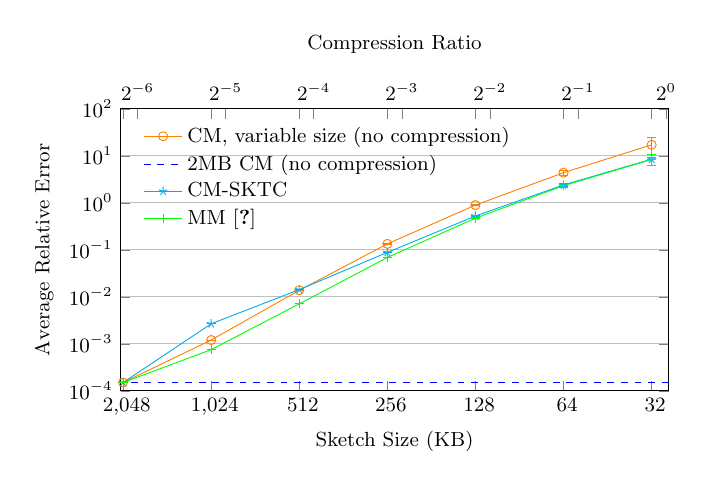
\begin{tikzpicture}[font=\small, scale=\myScale]

\begin{axis}[
        scale only axis,
        xlabel={Sketch Size (KB)},
        ylabel={Average Relative Error},
        xmode=log,
        log basis x=2,
        ymode=log,
        log basis y=10,
        ytick={0.0001,0.001,0.01,0.1,1,10,100},
        % log ticks with fixed point,
        xmin=28,
        xmax=2090,
        ymin= 0.0001,
        ymax = 100,
        ymajorgrids,
        x dir=reverse,
        xticklabel={
        \pgfkeys{/pgf/fpu=true}
        \pgfmathparse{int(2^\tick)}
        \pgfmathprintnumber[fixed]{\pgfmathresult}
        },
        height = 2*0.18 \columnwidth,
        width = 2*0.35 \columnwidth,
        legend style={at={(0.38,0.97)},anchor=north, draw=none, fill=none},
        legend cell align={left}
    ]
    

    \addplot[color=orange, mark=o, error bars/.cd, y dir=both, y explicit relative] coordinates {
        (32,17.2301386655751)+=(32,0.456273716855175)-=(32,0.456273716855175)
        (64,4.39851276684124)+=(64,0.125194135451736)-=(64,0.125194135451736)
        (128,0.897817799438924)+=(128,0.0331188667190209)-=(128,0.0331188667190209)
        (256,0.134055977504855)+=(256,0.0101784884960035)-=(256,0.0101784884960035)
        (512,0.0137905579843333)+=(512,0.00258244268887848)-=(512,0.00258244268887848)
        (1024,0.00120311464471896)+=(1024,0.000617359130580432)-=(1024,0.000617359130580432)
        (2048,0.000149737707752551)+=(2048,0.000271013920590392)-=(2048,0.000271013920590392)
    };
    \addlegendentry{CM, variable size (no compression)}
    
    \addplot [color=blue, domain=28:2090, dashed] {0.000149737707752551};
    \addlegendentry{2MB CM (no compression)}
    \addplot[color=cyan, mark=star, error bars/.cd, y dir=both, y explicit relative] coordinates {
        (32,8.50763586140085)+=(32,0.260338789864091)-=(32,0.260338789864091)
        (64,2.41233720425902)+=(64,0.0811565432460121)-=(64,0.0811565432460121)
        (128,0.524980932282619)+=(128,0.0282927869416904)-=(128,0.0282927869416904)
        (256,0.0883494285351726)+=(256,0.00848242056753894)-=(256,0.00848242056753894)
        (512,0.0142551949578031)+=(512,0.00276276859634349)-=(512,0.00276276859634349)
        (1024,0.00267072482933362)+=(1024,0.00102240698590769)-=(1024,0.00102240698590769)
        (2048,0.000149737707752551)+=(2048,0.000271013920590392)-=(2048,0.000271013920590392)
    };
    \addlegendentry{CM-SKTC}

    \addplot[color=green, mark=+, error bars/.cd, y dir=both, y explicit relative] coordinates {
        (32,8.39710896896061)+=(32,0.265442012913497)-=(32,0.265442012913497)
        (64,2.32340612291331)+=(64,0.0785598660178268)-=(64,0.0785598660178268)
        (128,0.473333620715826)+=(128,0.023338511940957)-=(128,0.023338511940957)
        (256,0.0688385614051386)+=(256,0.00833248009924655)-=(256,0.00833248009924655)
        (512,0.00708697096724866)+=(512,0.00213546569353468)-=(512,0.00213546569353468)
        (1024,0.000751364202893397)+=(1024,0.000553457068376218)-=(1024,0.000553457068376218)
        (2048,0.000149737707752551)+=(2048,0.000271013920590392)-=(2048,0.000271013920590392)
    };
    \addlegendentry{MM~\cite{yang2018elastic}}
    
    
\end{axis}
\begin{axis}[
  scale only axis,
  xlabel={Compression Ratio},
    x label style={at={(axis description cs:0.5,1.29)},anchor=north},
  xmin=28/2048,xmax=2090/2048,
  xmode=log,
  log basis x=2,
  ymin= 0.001,
  ymax = 100,
  axis y line=none,
  axis x line*=top,
  %xticklabels={$1$, $1$, $1/2$, $1/4$, $1/8$, $1/16$, $1/32$, $1/64$},
  height = 2*0.18 \columnwidth,
  width = 2*0.35 \columnwidth,]
\end{axis}
\end{tikzpicture}
\caption{Single node: Compression methods comparison}\label{sktc-fig:general-method-comparison}
\end{figure}

Figure \ref{sktc-fig:general-method-comparison} compares the different compression methods for different sketch sizes. The blue-dashed baseline represents the \textit{ARE} of the 2 MB CM sketch that both compression methods initiate from. One can observe that CM-SKTC outperforms the two other methods consistently. Furthermore, as the compression ratio decreases and the summary size increases, the \textit{ARE} improves, as expected.

\begin{figure}[!htb]
\centering
% This file was created by tikzplotlib v0.8.7.
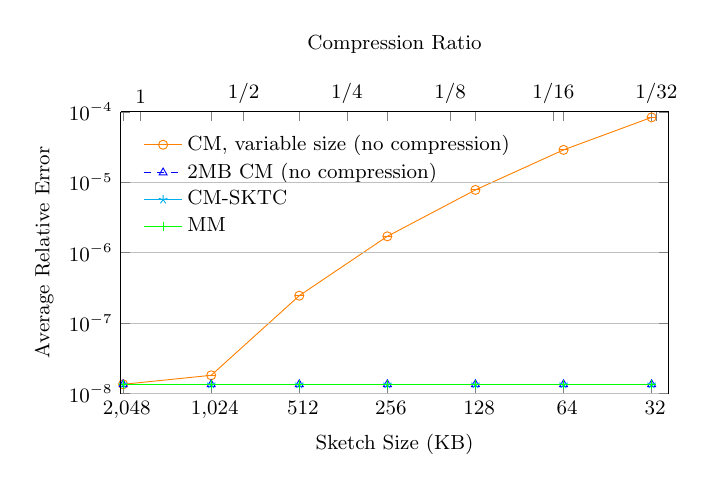
\begin{tikzpicture}[font=\small, scale=\myScale]

\begin{axis}[
        scale only axis,
        xlabel={Sketch Size (KB)},
        ylabel={Average Relative Error},
        xmode=log,
        log basis x=2,
        ymode=log,
        log basis y=10,
        xmin=28,
        xmax=2090,
        ymin= 10e-8,
        ymax = 10e-3,
        ymajorgrids,
        axis y line=none,
        log ticks with fixed point,
        x dir=reverse,
        xticklabel={
        \pgfkeys{/pgf/fpu=true}
        \pgfmathparse{int(2^\tick)}
        \pgfmathprintnumber[fixed]{\pgfmathresult}
        },
        height = 2*0.18 \columnwidth,
        width = 2*0.35 \columnwidth,
        legend style={at={(0.38,0.95)},anchor=north, draw=none, fill=none},
        legend cell align={left}
    ]
    
    %Change this line to single line without points (Also Figure 5), extend to 2048
    
    \addplot[color=orange, mark=o, error bars/.cd, y dir=both, y explicit relative] coordinates {
(32,0.00795579363029106)+=(32,0.00162895737328799)-=(32,0.00162895737328799)
(64,0.00210953168746669)+=(64,0.000599802582637658)-=(64,0.000599802582637658)
(128,0.000411176282548868)+=(128,0.000137097717563645)-=(128,0.000137097717563645)
(256,6.17486343494554E-05)+=(256,5.21386879346016E-05)-=(256,5.21386879346016E-05)
(512,5.45813819295529E-06)+=(512,1.28323308856708E-05)-=(512,1.28323308856708E-05)
(1024,2.11168238388759E-07)+=(1024,9.04130906579136E-07)-=(1024,9.04130906579136E-07)
(2048,0.000000146090104)+=(2048,5.91256371062124E-07)-=(2048,5.91256371062124E-07)
    };
    \addlegendentry{CM, variable size (no compression)}
    
    \addplot[color=blue, dashed, mark=triangle ,mark options={solid}] coordinates {
        (32,0.000000146090104) += (32,0.000271013920590392) -= (32,0.000271013920590392)
        (64,0.000000146090104) += (64,0.000271013920590392) -= (64,0.000271013920590392)
        (128,0.000000146090104) += (128,0.000271013920590392) -= (128,0.000271013920590392)
        (256,0.000000146090104) += (256,0.000271013920590392) -= (256,0.000271013920590392)
        (512,0.000000146090104) += (512,0.000271013920590392) -= (512,0.000271013920590392)
        (1024,0.000000146090104) += (1024,0.000271013920590392) -= (1024,0.000271013920590392)
        (2048,0.000000146090104) += (2048,0.000271013920590392) -= (2048,0.000271013920590392)
    };
    \addlegendentry{2MB CM (no compression)}
    
    \addplot[color=cyan, mark=star, error bars/.cd, y dir=both, y explicit relative] coordinates {
        (32,0.000000146090104) += (32,0.000271013920590392) -= (32,0.000271013920590392)
        (64,0.000000146090104) += (64,0.000271013920590392) -= (64,0.000271013920590392)
        (128,0.000000146090104) += (128,0.000271013920590392) -= (128,0.000271013920590392)
        (256,0.000000146090104) += (256,0.000271013920590392) -= (256,0.000271013920590392)
        (512,0.000000146090104) += (512,0.000271013920590392) -= (512,0.000271013920590392)
        (1024,0.000000146090104) += (1024,0.000271013920590392) -= (1024,0.000271013920590392)
        (2048,0.000000146090104) += (2048,0.000271013920590392) -= (2048,0.000271013920590392)
    };
    \addlegendentry{CM-SKTC}

    \addplot[color=green, mark=+, error bars/.cd, y dir=both, y explicit relative] coordinates {
        (32,0.000000146090104) += (32,0.000271013920590392) -= (32,0.000271013920590392)
        (64,0.000000146090104) += (64,0.000271013920590392) -= (64,0.000271013920590392)
        (128,0.000000146090104) += (128,0.000271013920590392) -= (128,0.000271013920590392)
        (256,0.000000146090104) += (256,0.000271013920590392) -= (256,0.000271013920590392)
        (512,0.000000146090104) += (512,0.000271013920590392) -= (512,0.000271013920590392)
        (1024,0.000000146090104) += (1024,0.000271013920590392) -= (1024,0.000271013920590392)
        (2048,0.000000146090104) += (2048,0.000271013920590392) -= (2048,0.000271013920590392)
    };
    \addlegendentry{MM}
    
    
\end{axis}
\begin{axis}[
  scale only axis,
  xlabel={Compression Ratio},
  ylabel={Average Relative Error},
  x label style={at={(axis description cs:0.5,1.3)},anchor=north},
  xmin=28/2048,xmax=1111/2048,
  xmode=log,
  log basis x=2,
  ymode=log,
ymin= 10e-9,
ymax = 10e-5,
ymajorgrids,
  axis x line*=top,  
  xticklabels={$1$, $1$, $1/2$, $1/4$, $1/8$, $1/16$, $1/32$, $1/64$},
  ytick={0.0001,0.00001, 0.000001, 0.0000001, 0.00000001},
  height = 2*0.18 \columnwidth,
  width = 2*0.35 \columnwidth,]
\end{axis}
\end{tikzpicture}

\caption{Single node: Compression methods comparison - top 50 flows. The 2MB-CM, CM-SKTC, and MM lines coalesce.}\label{sktc-fig:top50-method-comparison}
\end{figure}

In Figure \ref{sktc-fig:top50-method-comparison} we depict the same comparison as Figure \ref{sktc-fig:general-method-comparison}; however we choose a larger sample size of flows, and only to the 50 largest flows \textit{ARE} in each trace are considered. In this graph, one can observe that the top flows \textit{ARE} is extremely low for all methods. Moreover, the MM and CM-SKTC curves are similar, and both have the same error as the 2MB sketch.


%In Table \ref{sktc-table:evaluation:running_times} we compare the time of both the compression process and the query of the MM and CM-SKTC compression.
\inblue{Note that,} the MM is more time-efficient than the CM-SKTC compression. This is due to each hash being calculated twice (for the insertion and for the compression), and therefore we expect the CM-SKTC to be roughly twice as slow as the MM. \inred{Table~\ref{sktc-table:evaluation:data-sent} shows that our compression scheme has a lower packet overhead than MM. While MM may be faster, we can reduce the bandwidth used by the sketch significantly.}

From Figures \ref{sktc-fig:general-method-comparison} and \ref{sktc-fig:top50-method-comparison}, we deduce that the CM-SKTC has two important traits: (1) CM-SKTC achieves estimations within the required error parameters using smaller summaries, and (2) For large (elephant) flows this error is negligible.

\subsection{TA-CM with two ingestion nodes ($n=2$)}
\label{sktc-ssc:eval:TA-CM:2}
We now simulate two local nodes receiving a data stream of size $N$, where the relation between the size of the data stream $N_1$ processed at the first node, and the size of the data stream $N_2$ at the second node is $k=\frac{N_1}{N_2}$. We evaluate the effect of $k$ on the \textit{ARE}. 

Figure \ref{sktc-fig:two-servers-distribution} depicts the \textit{ARE} of merging two sketches when sending different sizes over the network. We compare locally building two sketches with error $\epsilon$, such that they each have size $1$MB (meaning $2$MB of data is sent over the network), and building larger local sketches with error $\sigma \epsilon$ and compressing them. We compare the trivial compression by factor $1 / \sigma$ compared to using our optimal resize factors, for $\sqrt{k}=3,7,10$. Note that our comparison shows that the error of resizing using optimal factors falls in between the error of starting with error $\epsilon$ and trivially compressing with error $\sigma \epsilon$. Of great importance is that even in the worst case the error is less than $\epsilon$. Table \ref{sktc-table:evaluation:data-sent} compares the summaries size across the network. It follows that there is a trade-off between the accuracy and the summaries size.
Figure \ref{sktc-fig:data-sent-ratio} shows the ratio between summaries size as a function of $k$, in relation to trivial compression.

\begin{figure}[!t]
\centering
% This file was created by tikzplotlib v0.8.7.
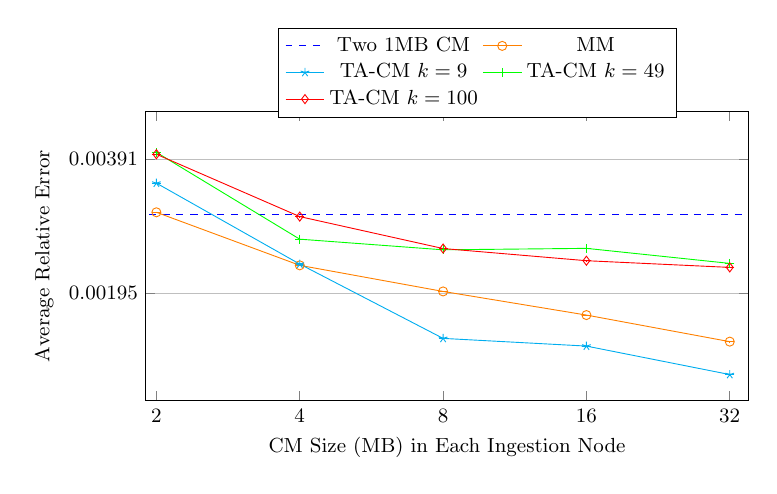
\begin{tikzpicture}[font=\small, scale=\myScale]

\begin{axis}[
        xlabel={CM Size (MB) in Each Ingestion Node},
        ylabel={Average Relative Error},
        xmode=log,
        log basis x=2,
        ymode=log,
        log basis y=2,
        log ticks with fixed point,
        xmin=1.9,
        xmax=35,
        ymin= 0,
        ymax = 0.005,
        ymajorgrids,
        height = 2*0.25 \columnwidth,
        width = 2*0.45 \columnwidth,
        legend style={at={(0.55,1.29)},anchor=north},
        legend columns = 2
        legend width = 2*0.35
        % mark repeat=5,
    ]
    
    \addplot [color=blue, domain=1:35, dashed] {0.002931419};
    \addlegendentry{Two 1MB CM}

    \addplot[color=orange, mark=o, error bars/.cd, y dir=both, y explicit relative] coordinates {
        (2,0.00296915803480048)+=(2,0.000347110578138022)-=(2,0.000347110578138022)
        (4,0.002256303092097967)+=(4,0.000358129292794643)-=(4,0.000358129292794643)
        (8,0.001971592412154686)+=(8,0.000367505249328563)-=(8,0.000367505249328563)
        (16,0.0017443431490592135)+=(16,0.000369607765498873)-=(16,0.000369607765498873)
        (32,0.001520224889699387)+=(32,0.000448184951568447)-=(32,0.000448184951568447)
    };
    \addlegendentry{MM}
    
    \addplot[color=cyan, mark=star, error bars/.cd, y dir=both, y explicit relative] coordinates {
        (2,0.0034529583824306)+=(2,0.000859556663510899)-=(2,0.000859556663510899)
        (4,0.00227091006184114)+=(4,0.00108749299593454)-=(4,0.00108749299593454)
        (8,0.00154598340803716)+=(8,0.000473362436844997)-=(8,0.000473362436844997)
        (16,0.00148559916036538)+=(16,0.000431282460768933)-=(16,0.000431282460768933)
        (32,0.00128208372348584)+=(32,0.0003850265319484)-=(32,0.0003850265319484)
    };
    \addlegendentry{TA-CM $k=9$}
    
    \addplot[color=green, mark=+, error bars/.cd, y dir=both, y explicit relative] coordinates {
        (2,0.00404911795243449)+=(2,0.000949957428845652)-=(2,0.000949957428845652)
        (4,0.00258340366490199)+=(4,0.000740916941009595)-=(4,0.000740916941009595)
        (8,0.00244495913594148)+=(8,0.00056656960414439)-=(8,0.00056656960414439)
        (16,0.00246352697587617)+=(16,0.000733011180075582)-=(16,0.000733011180075582)
        (32,0.00227907488232002)+=(32,0.000563417808543281)-=(32,0.000563417808543281)
    };
    \addlegendentry{TA-CM $k=49$}
    
    \addplot[color=red, mark=diamond, error bars/.cd, y dir=both, y explicit relative] coordinates {
(2,0.00400958809069177)+=(2,0.000782754740222883)-=(2,0.000782754740222883)
(4,0.00290372943567313)+=(4,0.000722232777089102)-=(4,0.000722232777089102)
(8,0.00246138051393235)+=(8,0.000502715484257819)-=(8,0.000502715484257819)
(16,0.00231092449094757)+=(16,0.000808776961871573)-=(16,0.000808776961871573)
(32,0.00223232953999738)+=(32,0.000394832438639461)-=(32,0.000394832438639461)
    };
    \addlegendentry{TA-CM $k=100$}
    
\end{axis}
\end{tikzpicture}

\caption{Two nodes: Compression methods comparison}\label{sktc-fig:two-servers-distribution}

\end{figure}

\begin{figure}[!t]
\centering
% This file was created by tikzplotlib v0.8.7.
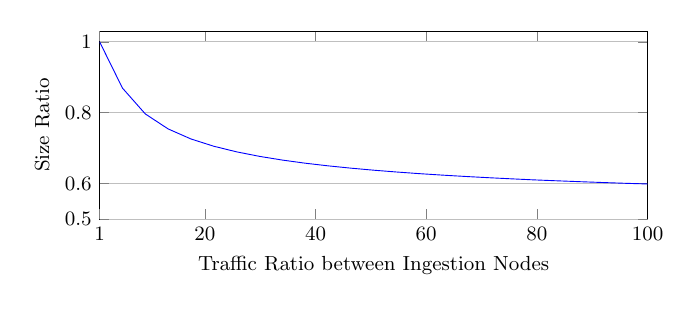
\begin{tikzpicture}[font=\small, scale=\myScale]

\begin{axis}[
        scale only axis,
        xlabel={Traffic Ratio between Ingestion Nodes},
        ylabel={Size Ratio},
        log ticks with fixed point,
        xmin=1,
        xmax=100,
        ymin= 0.5,
        ymax = 1.03,
        ymajorgrids,
        height = 0.24 \columnwidth,
        width = 2*0.35 \columnwidth,
        legend style={at={(0.8,0.6)},anchor=north, draw=none},
        extra x ticks ={1},
        extra y ticks ={0.5},
    ]
    
    \addplot+[blue, mark=none,domain=1:100] {(x^(1/2)+1)^2)/(2*(x+1)};
\end{axis}
\end{tikzpicture}
\caption{Ratio between summaries size in multiple compression methods 
}\label{sktc-fig:data-sent-ratio}
\end{figure}

\begin{table}[!t]
\caption{Compression Ratio by $k$ \label{sktc-table:evaluation:data-sent}}
    \centering
	\begin{tabular}{|c|c|}
	    \hline
		 \textbf{\shortstack{Compression \\ Method}}  & \textbf{\shortstack{Summaries Size Sent \\ (\% from max)}} \\ 
		\hline
		Maximum Merging & 2 MB (100\%)  \\ 
		\hline
		TA-CM, $k=1$ & 2 MB (100\%)  \\ 
		\hline
		TA-CM, $k=9$ & 1.6 MB (80\%)  \\ 
		\hline
		TA-CM, $k=49$ & 1.28 MB (64.3\%)  \\ 
		\hline
		TA-CM, $k=100$ & 1.18 MB (59\%)  \\ 
		\hline
	\end{tabular}
	 
%	\vspace{-6mm}
\end{table}

In Figure \ref{sktc-fig:two-servers-distribution-2MB} we show the results of compressing the same base CM sketch as in Figure \ref{sktc-fig:two-servers-distribution}. However, in this simulation, we compare the results when the total summaries size is $2$MB, i.e., the summaries account for $2$MB of network traffic. In this case, we observe that the TA-CM \textit{ARE} is better than the MM \textit{ARE}. TA-CM outperforms MM as it is traffic-aware and considers the distribution across the nodes and calculates the ratios accordingly; it helps to send the larger part of the data from the node that handled the larger chunk of the stream.

\begin{figure}[!t]
\centering
% This file was created by tikzplotlib v0.8.7.
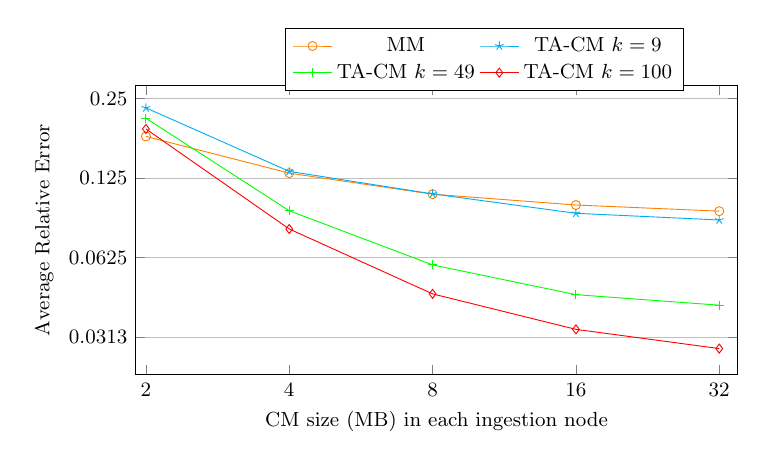
\begin{tikzpicture}[font=\small, scale=\myScale]

\begin{axis}[
        xlabel={CM size (MB) in each ingestion node},
        ylabel={Average Relative Error},
        xmode=log,
        log basis x=2,
        ymode=log,
        log basis y=2,
        log ticks with fixed point,
        xmin=1.9,
        xmax=35,
        ymin= 0,
        ymax = 0.28,
        ymajorgrids,
        height = 2*0.25 \columnwidth,
        width = 2*0.45 \columnwidth,
        legend style={at={(0.58,1.20)},anchor=north},
        legend columns = 2
        legend width = 2*0.35 \columnwidth,
        % mark repeat=5,
    ]
    
    \addplot[color=orange, mark=o] coordinates {
        (2,0.179743449)
        (4,0.130527461)
        (8,0.108661266)
        (16,0.098897622)
        (32,0.093743353)
    };
    \addlegendentry{MM}
    
    \addplot[color=cyan, mark=star] coordinates {
        (2,0.230504062225623)
        (4,0.13258234871128)
        (8,0.108942408575435)
        (16,0.0920066621666375)
        (32,0.0867979682007765)
    };
    \addlegendentry{TA-CM $k=9$}
    
    \addplot[color=green, mark=+] coordinates {
        (2,0.210633144817792)
        (4,0.0940809172884923)
        (8,0.0586891464861655)
        (16,0.0452908789372009)
        (32,0.0413224013064837)
    };
    \addlegendentry{TA-CM $k=49$}
    
    \addplot[color=red, mark=diamond] coordinates {
        (2,0.191880649575314)
        (4,0.0802466257250163)
        (8,0.0455919938550279)
        (16,0.0334732122784799)
        (32,0.0283161105139431)
    };
    \addlegendentry{TA-CM $k=100$}
    
\end{axis}
\end{tikzpicture}

\caption{Two nodes: Compression methods comparison. Allowance of $2$MB sent from ingestion nodes to centralized server.} \label{sktc-fig:two-servers-distribution-2MB}

\end{figure}

\subsection{TA-CM with $n$ ingestion nodes}
\label{sktc-ssc:eval:TA-CM:n}
\begin{figure}[!htb]
\centering

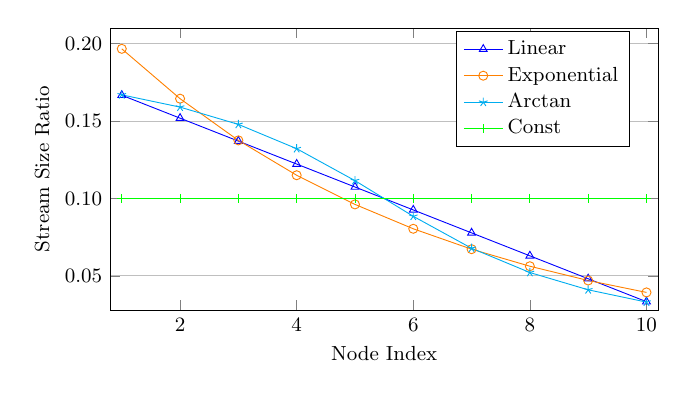
\begin{tikzpicture}[font=\small, scale=\myScale]

\begin{axis}[
        scale only axis,
        xlabel={Node Index},
        ylabel={Stream Size Ratio},
        xmin=0.8,
        xmax=10.2,
        ymin= 0.028,
        ymax = 0.21,
        ymajorgrids,
        yticklabel=\pgfkeys{/pgf/number format/.cd,fixed,precision=2,zerofill}\pgfmathprintnumber{\tick},
        height = 2*0.18 \columnwidth,
        width = 2*0.35 \columnwidth,
        legend style={at={(0.79,0.99)},anchor=north},
        legend cell align={left}
    ]
    %add ticks all x
    \addplot[color=blue, mark=triangle] coordinates {
        (1,0.166666667)
        (2,0.151851852)
        (3,0.137037037)
        (4,0.122222222)
        (5,0.107407407)
        (6,0.092592593)
        (7,0.077777778)
        (8,0.062962963)
        (9,0.048148148)
        (10,0.033333333)
    };
    \addlegendentry{Linear}

    \addplot[color=orange, mark=o] coordinates {
        (1,0.196636457)
        (2,0.16443744)
        (3,0.137510979)
        (4,0.114993698)
        (5,0.096163598)
        (6,0.080416908)
        (7,0.067248722)
        (8,0.056236813)
        (9,0.047028093)
        (10,0.039327291)
    };
    \addlegendentry{Exponential}
    
    \addplot[color=cyan, mark=star] coordinates {
        (1,0.16692565)
        (2,0.1589913)
        (3,0.14783371)
        (4,0.13215652)
        (5,0.11151949)
        (6,0.0884805)
        (7,0.06784347)
        (8,0.05216628)
        (9,0.04100869)
        (10,0.033074344)
    };
    \addlegendentry{Arctan}
    
    \addplot[color=green, mark=+] coordinates {
        (1,0.1)
        (2,0.1)
        (3,0.1)
        (4,0.1)
        (5,0.1)
        (6,0.1)
        (7,0.1)
        (8,0.1)
        (9,0.1)
        (10,0.1)
    };
    \addlegendentry{Const}
    
\end{axis}
\end{tikzpicture}
\caption{$n=10$ nodes: Stream size distribution over the nodes}\label{sktc-fig:10-servers-distribution}
\end{figure}

To evaluate TA-CM in multiple-ingestion nodes scenarios, we formulate four different types of distributions for 10 nodes (see Figure \ref{sktc-fig:10-servers-distribution}) and compare the TA-CM to MM and the non-compressed CM sketch. The distributions were chosen such that the ratio between the largest server ratio to the smallest server ratio is 5 (i.e., $N_1 / N_{10} = 5$).

The  CM sketch base size for each of the $10$ nodes is $32$KB. We compare the \textit{ARE} with multiple values of $\sigma$ (i.e., the ratio by which the ingestion node CM sizes is increased) and compressing with two methods: (1) TA-CM with ratios computed in Section \ref{sktc-sec:resize} (2) MM compression with all ratios are $1/\sigma$. As depicted in Figure~\ref{sktc-fig:10-servers-distribution-compression}, TA-CM achieves similar results in terms of \textit{ARE} to the Maximum Merging compression and improves the results of the basic non-compressed CM. However, it does so while decreasing the total summaries size.  Table \ref{sktc-table:evaluation:cr-distributions} indicates that the TA-CM saves between 7\% to 9\% of the total summaries size for chosen distributions. This saving ratio can be increased by choosing other, wider distributions of the stream (for example if the stream distributes across the ingestion nodes by Pareto distribution then TA-CM potentially saves an even higher percentage).

\begin{table}[!htb]
	\caption{Compression ratio of various distributions}

    \centering
	\begin{tabular}{|c|c|}
	    \hline
		\textbf{Distribution}  & \textbf{\shortstack{Summaries Size \\ (\% from max)}} \\ 
		\hline
		Maximum Merging & 320KB (100\%)  \\ 
		\hline
		Constant Dist. & 320KB (100\%)  \\ 
		\hline
		Exponential Dist. & $\sim$ 292KB (91.3\%)  \\ 
		\hline
		Linear Dist. & $\sim$ 298KB (93.3\%)  \\ 
		\hline
		Arctan Dist. & $\sim$ 293KB (91.6\%)  \\ 
		\hline
	\end{tabular}
	\label{sktc-table:evaluation:cr-distributions}
%	\vspace{-6mm}
\end{table}

\begin{figure}[!htb]
\centering

% This file was created by tikzplotlib v0.8.7.
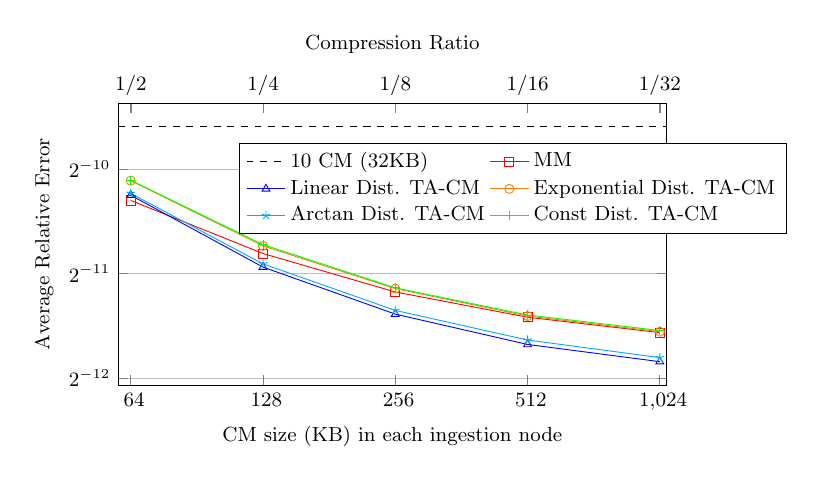
\begin{tikzpicture}[font=\small, scale=\myScale]

\begin{axis}[
        scale only axis,
        xlabel={CM size (KB) in each ingestion node},
        ylabel={Average Relative Error},
        xmode=log,
        log basis x=2,
        ymode=log,
        log basis y=2,
        xmin=60,
        xmax=1060,
        log ticks with fixed point,
        height = 2*0.18 \columnwidth,
        width = 2*0.35 \columnwidth,
        yticklabels={$2^{-13}$,$2^{-12}$, $2^{-11}$, $2^{-10}$},
        ymajorgrids,
        xticklabel={
        \pgfkeys{/pgf/fpu=true}
        \pgfmathparse{int(2^\tick)}
        \pgfmathprintnumber[fixed]{\pgfmathresult}
        },
        legend style={at={(0.72,0.86)},anchor=north},
        legend columns = 2,
        legend cell align={left}
    ]
    
    %change to fixed line
    \addplot [color=black, domain=60:1060, dashed] {0.001295165};
    \addlegendentry{10 CM (32KB)}

    \addplot[color=red, mark=square] coordinates {
        (64,0.000794505)
        (128,0.000558492)
        (256,0.000432703)
        (512,0.00036593)
        (1024,0.000330449)
    };
    \addlegendentry{MM}
    
    \addplot[color=blue, mark=triangle] coordinates {
        (64,0.000822598)
        (128,0.000510391)
        (256,0.000373544)
        (512,0.000305408)
        (1024,0.00027242)
    };
    \addlegendentry{Linear Dist. TA-CM}
    
    \addplot[color=orange, mark=o] coordinates {
        (64,0.000905932)
        (128,0.000587575)
        (256,0.000442481)
        (512,0.000368815)
        (1024,0.000332426)
    };
    \addlegendentry{Exponential Dist. TA-CM}
    
    \addplot[color=cyan, mark=star] coordinates {
        (64,0.000832502)
        (128,0.000521449)
        (256,0.000382919)
        (512,0.000314548)
        (1024,0.000279836)
    };
    \addlegendentry{Arctan Dist. TA-CM}
    
    \addplot[color=green, mark=+] coordinates {
        (64,0.000908105)
        (128,0.000592652)
        (256,0.000444668)
        (512,0.000371463)
        (1024,0.000335038)
    };
    \addlegendentry{Const Dist. TA-CM}
    
\end{axis}
\begin{axis}[
  scale only axis,
  xlabel={Compression Ratio},
    x label style={at={(axis description cs:0.5,1.27)},anchor=north},
  xmin=60/2048,xmax=1060/2048,
  xmode=log,
  log basis x=2,
  ymin= 0.001,
  ymax = 100,
  axis y line=none,
  axis x line*=top,
  xticklabels={$1$, $1/2$, $1/4$, $1/8$, $1/16$, $1/32$},
  height = 2*0.18 \columnwidth,
  width = 2*0.35 \columnwidth,]
\end{axis}

\end{tikzpicture}

\caption{$n=10$ nodes: Compression method comparison - various distributions}\label{sktc-fig:10-servers-distribution-compression}
\end{figure}

\subsection{TA-KMV with $n$ ingestion nodes}\label{sktc-subsec:eval:kmv}
%Replace the word record
%replace the word number with # in X labels
In this section, we evaluate \emph{TA-KMV}. We use the same method as in the previous section to generate the input stream. However, for this section, we use only the linear distribution. We compare our \emph{TA-KMV} with multiple compression ratios. The compression ratio is measured by \emph{Total Hash-values Sent (THS)}. To the best of our knowledge, no compression scheme is available for this sketch, and therefore we compare our method only to the baseline, i.e., each ingestion node sends $k$ hash values to the centralized server. Our measurement unit is the estimation precision rate to true cardinality. In this case, the number of hash values that are sent to the centralized server is $n \cdot k$, where $n$ is the number of ingestion nodes.

\begin{figure}[!htb]
\centering

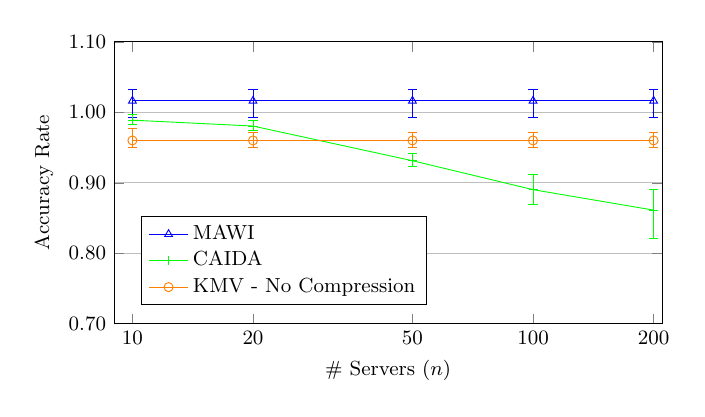
\begin{tikzpicture}[font=\small, scale=\myScale]

\begin{axis}[
        scale only axis,
        xlabel={\# Servers ($n$)},
        ylabel={Accuracy Rate},
        xmin=9,
        xmax=210,
        ymin= 0.70,
        ymajorgrids,
        ymax = 1.1,
        xmode=log,
        log ticks with fixed point,
        xtick = {5,10,20,50,100,200},
        yticklabel=\pgfkeys{/pgf/number format/.cd,fixed,precision=2,zerofill}\pgfmathprintnumber{\tick},
        height = 2*0.18 \columnwidth,
        width = 2*0.35 \columnwidth,
        legend style={at={(0.05,0.065)},anchor=south west},
        legend cell align={left}
    ]
    
    \addplot[color=blue, mark=triangle, error bars/.cd, y dir=both, y explicit relative] coordinates {
(10,1.01612079900443)  += (10,0.0157908595664422) -=(10,0.0224356127165992)
(20,1.01612079900443)  += (20,0.0162978598619865) -=(20,0.0224356127165992)
(50,1.01612079900443)  += (50,0.0162978598619865) -=(50,0.0224356127165992)
(100,1.01612079900443)  += (100,0.0162978598619865) -=(100,0.0224356127165992)
(200,1.01612079900443)  += (200,0.0162978598619865) -=(200,0.0224356127165992)
    };
    \addlegendentry{MAWI}
    
    \addplot[color=green, mark=+, error bars/.cd, y dir=both, y explicit relative] coordinates {
(10,0.988813459783557)  += (10,0.00800539555909119) -=(10,0.00595529407844508)
(20,0.980463796203664)  += (20,0.00830907805368898) -=(20,0.00658938198094061)
(50,0.931249963187018)  += (50,0.0109794749801466) -=(50,0.00797865392094566)
(100,0.890186318982447)  += (100,0.0235224353515718) -=(100,0.0234221082610149)
(200,0.861126139373611)  += (200,0.0342711777766666) -=(200,0.0462573349075841)
    };
    \addlegendentry{CAIDA}
    
    \addplot[color=orange, mark=o, error bars/.cd, y dir=both, y explicit relative] coordinates {
(10,0.960038171361342)  += (10,0.0174336347135434) -=(10,0.0110330067979534)
(20,0.960038171361342)  += (20,0.0124716598206064) -=(20,0.0110330067979534)
(50,0.960038171361342)  += (50,0.0124716598206064) -=(50,0.0110330067979534)
(100,0.960038171361342)  += (100,0.0124716598206064) -=(100,0.0110330067979534)
(200,0.960038171361342)  += (200,0.0124716598206064) -=(200,0.0110330067979534)
    };
    \addlegendentry{KMV - No Compression}
    
\end{axis}

\end{tikzpicture}



\caption{TA-KMV vs baseline for $k=1024$.} \label{sktc-fig:kmv-sktc-eval}
\end{figure}

% \begin{table}[!htb]
% 	\caption{Records sent for various compression methods}

%     \centering
% 	\begin{tabular}{|c|c|}
% 	    \hline
% 		\textbf{Plot}  & \textbf{\shortstack{THS sent for 200 ingestion nodes \\ (\% from max)}} \\ 
% 		\hline
% 		KMV - No Compression & 204800 (100\%)  \\ 
% 		\hline
% 		\emph{TA-KMV, THS}=$k\ln{k}$ & 7498 ( $\sim$ 3.6\%)  \\ 
% 		\hline
% 		\emph{TA-KMV, THS}=$2k\ln{k}$ & 14596 ( $\sim$ 7.1\%)  \\ 
% 		\hline
% 	\end{tabular}
% 	\label{sktc-table:evaluation:sktc-kmv}
% \end{table}

Figure \ref{sktc-fig:kmv-sktc-eval} depicts the impact of the number of ingestion nodes on the accuracy rate of TA-KMV, \inred{with the confidence interval}. We define the accuracy rate as $\frac{\text{Estimation}}{\text{\# Flows}}$. \inblue{The figure shows that the estimation remains fairly accurate even at $100$ nodes. The CAIDA dataset does not have many flows, therefore the aggregate ends up receiving multiples of the same hash value, and thus the \inred{accuracy begins to drop}. For example, at 200 nodes the central server receives only 300 different hash values. Contrast this with MAWI, where, due to the larger number of small flows, the central server receives all 1024 of the smallest hash values. Consider the case of $50$ nodes. The baseline sends $51200$ hash values, whereas the compressed version send around $4150$ hash values -- a $92\%$ decrease for a near negligible decrease in accuracy. This creates a clear trade-off between the accuracy rate and the total summaries size. We note that sending less than $k \ln k$ hash values in total (e.g., $k$) greatly reduced the accuracy of the estimation.}
%In Table \ref{sktc-table:evaluation:sktc-kmv} we show that  although TA-KMV accuracy slightly decreased, it saves more than 90\% of the total hash values sent over the network.
%It allows network operators to decide whether they prefer to lose some accuracy and increase the possible bandwidth over the network, or increase the accuracy and pay more in management packets.


\subsection{TA-HLL with $n$ ingestion nodes}



\label{sktc-ssc:eval:TA-HLL}
Lastly, we compare the  four methods for traffic aware cardinality estimation using compression of distributed HLL described in Section~\ref{sktc-sec:hll}. Recall that the methods are: 

\emph{(i)} (Random) Each node reports each of its counters w.p. $p$.

\emph{(ii)} (Weighted) Reporting a counter value $c$ w.p. $p_c$.

\emph{(iii)} (Largest) Each node reports its  $\beta \cdot m$ largest counters.

\emph{(iv)} (Threshold) Each node reports all its counters with values of at least a threshold $c_T$.

We evaluate the results of these four methods with an HLL array with size 128, using the CAIDA and MAWAI datasets. We evaluate all the four methods through two metrics for accuracy: The first metric is the centralized node Array Recovery Rate given as the percentage of cells in the centralized node recovered array that are identical to the corresponding cells in a HLL sketch that could be computed over all network traffic. The second evaluated metric is the relative error: For a distributed HLL estimation $C$, and real stream cardinality $F$,  the relative error is $RE = \frac{|F-C|}{F}$. We first consider 10 ingestion nodes (and later vary their number).

\begin{figure}[t!]
\centering

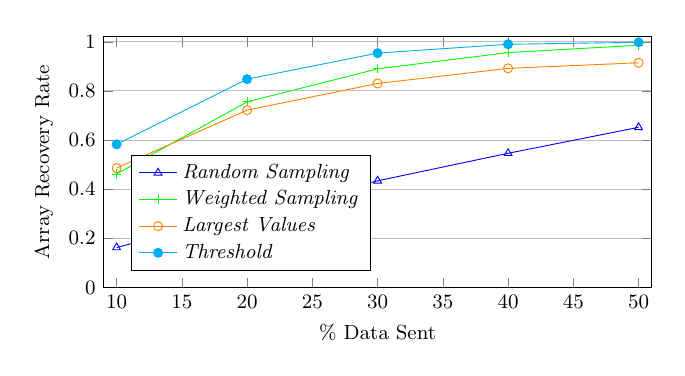
\begin{tikzpicture}[font=\small, scale=\myScale]

\begin{axis}[
        scale only axis,
        xlabel={\% Data Sent},
        ylabel={Array Recovery Rate},
        xmin=9,
        xmax=51,
        ymin= 0,
        ymajorgrids,
        ymax = 1.02,
        height = 2*0.16 \columnwidth,
        width = 2*0.35 \columnwidth,
        legend style={at={(0.05,0.065)},anchor=south west},
        legend cell align={left}
    ]
    
    \addplot[color=blue, mark=triangle, error bars/.cd, y dir=both, y explicit relative] coordinates {
        (10,0.162523674242424)
        (20,0.302260890151515)
        (30,0.434067234848485)
        (40,0.546223958333333)
        (50,0.651811079545455)
    };
    \addlegendentry{\emph{Random Sampling}}
    
    \addplot[color=green, mark=+, error bars/.cd, y dir=both, y explicit relative] coordinates {
        (10,0.46194365530303)
        (20,0.755563446969697)
        (30,0.889973958333333)
        (40,0.956143465909091)
        (50,0.986032196969697)
    };
    \addlegendentry{\emph{Weighted Sampling}}
    
    \addplot[color=orange, mark=o, error bars/.cd, y dir=both, y explicit relative] coordinates {
        (10,0.486100852272727)
        (20,0.721960227272727)
        (30,0.830331439393939)
        (40,0.89188446969697)
        (50,0.914670928030303)
    };
    \addlegendentry{\emph{Largest Values}}
    
    \addplot[color=cyan, mark=*, error bars/.cd, y dir=both, y explicit relative] coordinates {
        (10,0.582682291666667)
        (20,0.848070549242424)
        (30,0.953953598484849)
        (40,0.990056818181818)
        (50,0.998046875)
    };
    \addlegendentry{\emph{Threshold}}
    
\end{axis}

\end{tikzpicture}

\caption{TA-HLL Array Recovery Rate in CAIDA -- 10 ingestion nodes} \label{sktc-fig:eval-hll-arr}
\end{figure}

\begin{figure}[t!]
\centering

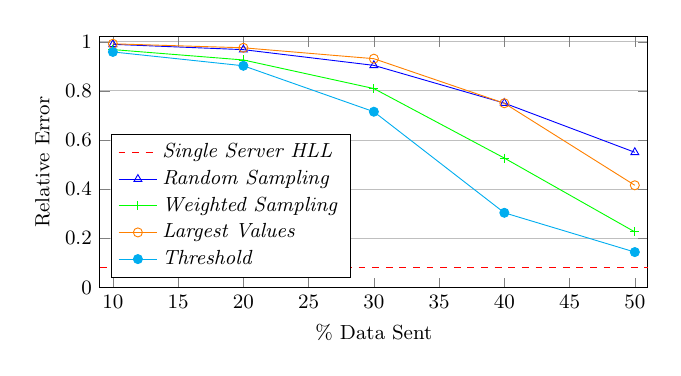
\begin{tikzpicture}[font=\small, scale=\myScale]

\begin{axis}[
        scale only axis,
        xlabel={\% Data Sent},
        ylabel={Relative Error},
        xmin=9,
        xmax=51,
        ymin= 0,
        ymajorgrids,
        ymax = 1.02,
        height = 2*0.16 \columnwidth,
        width = 2*0.35 \columnwidth,
        legend style={at={(0.02,0.04)},anchor=south west},
        legend cell align={left}
    ]
    
    \addplot [color=red, domain=9:210, dashed] {0.081807084};
    \addlegendentry{\emph{Single Server HLL}}
    
    \addplot[color=blue, mark=triangle, error bars/.cd, y dir=both, y explicit relative] coordinates {
        (10,0.989818001815833)
        (20,0.968150415942164)
        (30,0.904137272470303)
        (40,0.750498757765852)
        (50,0.550173699201597)
    };
    \addlegendentry{\emph{Random Sampling}}
    
    \addplot[color=green, mark=+, error bars/.cd, y dir=both, y explicit relative] coordinates {
        (10,0.968407356663112)
        (20,0.926128690744725)
        (30,0.809747424055189)
        (40,0.526700142191625)
        (50,0.226103519616794)
    };
    \addlegendentry{\emph{Weighted Sampling}}
    
    \addplot[color=orange, mark=o, error bars/.cd, y dir=both, y explicit relative] coordinates {
        (10,0.991935446090819)
        (20,0.975726704254263)
        (30,0.931307572956268)
        (40,0.749948665319353)
        (50,0.415925436754393)
    };
    \addlegendentry{\emph{Largest Values}}
    
    \addplot[color=cyan, mark=*, error bars/.cd, y dir=both, y explicit relative] coordinates {
        (10,0.958849167188452)
        (20,0.902461336487268)
        (30,0.715378351707372)
        (40,0.303923157641182)
        (50,0.144018817238216)
    };
    \addlegendentry{\emph{Threshold}}
    
\end{axis}

\end{tikzpicture}



\caption{TA-HLL Relative Error in CAIDA -- 10 ingestion nodes} \label{sktc-fig:eval-hll-re}
\end{figure}





Figure \ref{sktc-fig:eval-hll-arr} shows the Array Recovery Rate for  the four methods, as a function of percentage of data sent across the network as part of all ingestion nodes HLL array sizes. Here, with 10 ingestion nodes and HLL array size of 128, the total size is 1280. 
For instance, 20\% means sending a total of 256 values to the centralized server. 
We can see that methods Weighted sampling (ii) and Threshold (iv) that require an iterative process with the centralized server achieve higher accuracy. 

\begin{figure}[b!]
\centering

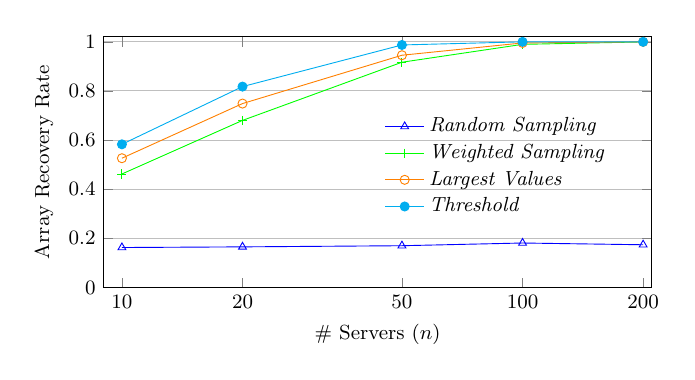
\begin{tikzpicture}[font=\small, scale=\myScale]

\begin{axis}[
        scale only axis,
        xlabel={\# Servers ($n$)},
        ylabel={Array Recovery Rate},
        xmin=9,
        xmax=210,
        ymin= 0,
        ymajorgrids,
        ymax = 1.02,
        xmode=log,
        log ticks with fixed point,
        xtick = {5,10,20,50,100,200},
        height = 2*0.16 \columnwidth,
        width = 2*0.35 \columnwidth,
        legend style={at={(0.5,0.25)},anchor=south west, draw=none, opacity=1, fill=none},
        legend cell align={left}
    ]
    
    \addplot[color=blue, mark=triangle, error bars/.cd, y dir=both, y explicit relative] coordinates {
        (10,0.162523674242424)
        (20,0.165187026515152)
        (50,0.169862689393939)
        (100,0.180871212121212)
        (200,0.173768939393939)
    };
    \addlegendentry{\emph{Random Sampling}}
    
    \addplot[color=green, mark=+, error bars/.cd, y dir=both, y explicit relative] coordinates {
        (10,0.46194365530303)
        (20,0.680101799242424)
        (50,0.916903409090909)
        (100,0.989701704545455)
        (200,0.999585700757576)
    };
    \addlegendentry{\emph{Weighted Sampling}}
    
    \addplot[color=orange, mark=o, error bars/.cd, y dir=both, y explicit relative] coordinates {
        (10,0.526100852272727)
        (20,0.748579545454545)
        (50,0.945371685606061)
        (100,0.995442708333333)
        (200,0.999881628787879)
    };
    \addlegendentry{\emph{Largest Values}}
    
    \addplot[color=cyan, mark=*, error bars/.cd, y dir=both, y explicit relative] coordinates {
        (10,0.582682291666667)
        (20,0.817708333333333)
        (50,0.987215909090909)
        (100,0.999940814393939)
        (200,1)
    };
    \addlegendentry{\emph{Threshold}}
    
\end{axis}

\end{tikzpicture}



\caption{TA-HLL Array Recovery Rate in CAIDA  -- 10\% data sent} \label{sktc-fig:eval-hll-in-arr}
\end{figure}

\begin{figure}[b!]
\centering

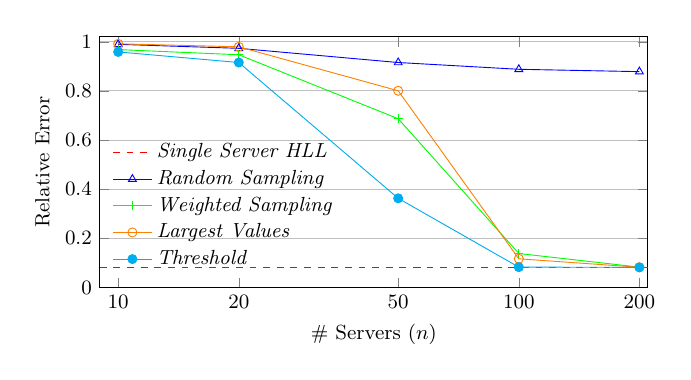
\begin{tikzpicture}[font=\small,scale=\myScale]

\begin{axis}[
        scale only axis,
        xlabel={\# Servers ($n$)},
        ylabel={Relative Error},
        xmin=9,
        xmax=210,
        ymin= 0,
        ymajorgrids,
        ymax = 1.02,
        xmode=log,
        log ticks with fixed point,
        xtick = {5,10,20,50,100,200},
        height = 2*0.16 \columnwidth,
        width = 2*0.35 \columnwidth,
        legend style={at={(0.01,0.04)},anchor=south west, draw=none, opacity=1, fill=none},
        legend cell align={left}
    ]
    
    \addplot [color=red, domain=9:210, dashed] {0.081807084};
    \addlegendentry{\emph{Single Server HLL}}
    
    \addplot[color=blue, mark=triangle, error bars/.cd, y dir=both, y explicit relative] coordinates {
        (10,0.989818001815833)
        (20,0.973515139894837)
        (50,0.91574909464158)
        (100,0.888143415446563)
        (200,0.87856880423703)
    };
    \addlegendentry{\emph{Random Sampling}}
    
    \addplot[color=green, mark=+, error bars/.cd, y dir=both, y explicit relative] coordinates {
        (10,0.968407356663112)
        (20,0.947318190605346)
        (50,0.686897917425959)
        (100,0.138120889057764)
        (200,0.0827054662824469)
    };
    \addlegendentry{\emph{Weighted Sampling}}
    
    \addplot[color=orange, mark=o, error bars/.cd, y dir=both, y explicit relative] coordinates {
        (10,0.991935446090819)
        (20,0.979722025039235)
        (50,0.800648090848471)
        (100,0.116603690823036)
        (200,0.0821491851664647)
    };
    \addlegendentry{\emph{Largest Values}}
    
    \addplot[color=cyan, mark=*, error bars/.cd, y dir=both, y explicit relative] coordinates {
        (10,0.958849167188452)
        (20,0.91577629304402)
        (50,0.36283955355022)
        (100,0.0827209569907977)
        (200,0.081807083923316)
    };
    \addlegendentry{\emph{Threshold}}
    
\end{axis}

\end{tikzpicture}



\caption{TA-HLL Relative Error in CAIDA - 10\% data sent} \label{sktc-fig:eval-hll-in-re}
\end{figure}

\begin{figure}[b!]
\centering

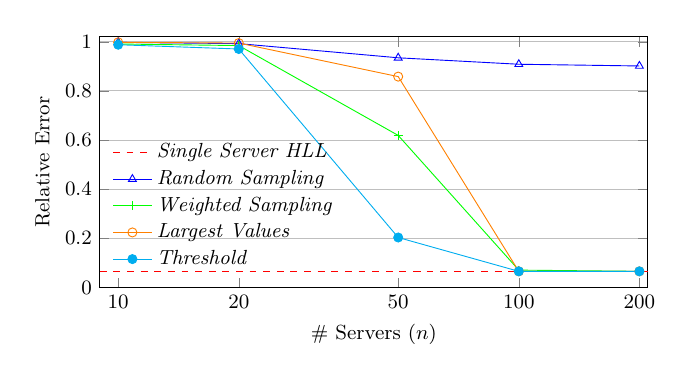
\begin{tikzpicture}[font=\small,scale=\myScale]

\begin{axis}[
        scale only axis,
        xlabel={\# Servers ($n$)},
        ylabel={Relative Error},
        xmin=9,
        xmax=210,
        ymin= 0,
        ymajorgrids,
        ymax = 1.02,
        xmode=log,
        log ticks with fixed point,
        xtick = {5,10,20,50,100,200},
        height = 2*0.16 \columnwidth,
        width = 2*0.35 \columnwidth,
        legend style={at={(0.01,0.04)},anchor=south west, draw=none, opacity=1, fill=none},
        legend cell align={left}
    ]
    
    \addplot [color=red, domain=9:210, dashed] {0.065548765};
    \addlegendentry{\emph{Single Server HLL}}
    
    \addplot[color=blue, mark=triangle, error bars/.cd, y dir=both, y explicit relative] coordinates {
        (10,0.997791172)
        (20,0.992680167)
        (50,0.934956428)
        (100,0.90867773)
        (200,0.901680999)
    };
    \addlegendentry{\emph{Random Sampling}}
    
    \addplot[color=green, mark=+, error bars/.cd, y dir=both, y explicit relative] coordinates {
        (10,0.991108609)
        (20,0.984747064)
        (50,0.61894103)
        (100,0.070554953)
        (200,0.065548765)
    };
    \addlegendentry{\emph{Weighted Sampling}}
    
    \addplot[color=orange, mark=o, error bars/.cd, y dir=both, y explicit relative] coordinates {
        (10,0.998044631)
        (20,0.99495585)
        (50,0.85833174)
        (100,0.065548765)
        (200,0.065548765)
    };
    \addlegendentry{\emph{Largest Values}}
    
    \addplot[color=cyan, mark=*, error bars/.cd, y dir=both, y explicit relative] coordinates {
        (10,0.988117335)
        (20,0.970737772)
        (50,0.203320455)
        (100,0.065548765)
        (200,0.065548765)
    };
    \addlegendentry{\emph{Threshold}}
    
\end{axis}

\end{tikzpicture}

\caption{\inblue{TA-HLL Relative Error in MAWI - 10\% data sent}} \label{sktc-fig:eval-hll-in-re-mawi}
\end{figure}

Figure \ref{sktc-fig:eval-hll-re} presents the relative error of the same scenario, and as one could assume, the two graphs show coordinated results, i.e., the best method in terms of Array Recovery Rate (Threshold) allows lower Relative Error.  
Note that computing the particular threshold values for each node might require a relatively complicated iterative process with the centralized server with potential tradeoff between the number of iterations and communication overhead.
%However, In our simulations we ignored the communication that is needed to find the threshold value to be the correct percentile, in contrary to the Weighted Sampling method, in which we did not ignore the data that sent to the centralized node before the probability calculations. Which means that in realistic scenarios the Weighted Sampling method is possibly better than Threshold method.




In Figures \ref{sktc-fig:eval-hll-in-arr}-\ref{sktc-fig:eval-hll-in-re-mawi}, we present the impact of the number of ingestion nodes across the network on accuracy. We used the same settings as described in previous figures, with only 10\% of the data sent to the centralized node and varied the number of ingestion nodes across the network. Once again the two methods with an iterative process with the centralized server are more accurate than the other two methods. Another observation is that as the number of ingestion nodes increases, the performance improves, that is because the total number of reports that arrive to the centralized node is increasing and as such, the probability to receive per each cell a value identical to that computed for the complete traffic is increasing as well.

\section{Conclusion}\label{sktc-sec:conclusion}
In this paper, we presented the problem of merging data from multiple measurement points to one centralized server, described a distributed traffic-aware sketching scheme, and applied it to three unique sketches. 
We presented the CM-SKTC sketch as a simple, yet efficient method for compressing the CM sketch to any desired size, then used this method to generate \emph{TA-CM}, a new scheme for flow-size measurements that 
%performs as well as previously presented methods 
provides high accuracy 
and  decreases the total summaries size sent to the centralized server by considering the traffic of each node. 
This method is important in today's network design because when the traffic congestion in the network is high the need to successfully measure the network load is higher. In such situations, the extra load created by sending the summaries can worsen network congestion. 

Moreover, we generalized this approach for cardinality estimation and introduced new traffic-aware designs of the KMV sketch as well as of the HLL sketch. They both send fewer values while retaining high accuracy cardinality estimation. 
Finally, we analyzed these sketches under multiple network settings and examined the trade-off between the accuracy and the size of summaries.

Several directions can be the focus in future work.  
%There are some topics we did not address and can be focused on in future work. 
A straightforward extension is developing compression algorithms for additional kinds of sketches %; there are many other types of sketches that 
allowing different measurement tasks (e.g., Quantiles for rank estimation~\cite{agarwal2013mergeable}).  
%Likewise, calculating the TA-KMV compression ratios only takes into account the estimated cardinality at ingestion nodes. It would be interesting to suggest other heuristics for deciding how many (and which) elements to send as part of the summary. For example, we can consider storing the element frequencies alongside the hashes -- as the frequency rises the less likely a node needs to send the specific hash as another node probably has the same element and will send it.
%Moreover, each of the presented compression schemes refers to a sketch supporting a single task such as flow size estimation or cardinality estimation. It is interesting to generalize the approach towards generic sketches such as UnivMon~\cite{liu2016one} and 
%NitroSketch~\cite{NitroSketch} supporting multiple tasks. This might involve definitions for ideal resize factors that refer jointly to multiple tasks, observing different types of errors with potential heterogeneous balance among the required size of summaries for the various nodes.
%Another interesting addition to this paper can be studying the impact of interleaving the ingestion nodes such that streams observed by the nodes might not be disjoint. This problem raises multiple questions related to duplicate handling of the system which we currently ignore by assuming that the ingestion nodes are separate. 
Likewise, we wish to design further compression of sketches 
by leveraging existing generic compression techniques such as Huffman codes, LZ77 or gzip~\cite{huffman1952method, ziv1977universal, deutsch1996gzip}. 


% \chapter{A main chapter}
\label{chap:firstchap}

\section{Introduction}

You might have a per-chapter mini-intro, possibly tying in to the relevant part of the general intro.

\section{A section}

\lipsum[1]

Let's cite a source: \cite{Yao1977}. And now,  let's introduce a (numbered) equation...
\begin{align}
\label{eq:emc2}
e &= mc^2
\end{align}

\begin{note}
	Are you seeing a problem with the equation numbering? In some TeX processors and on some platforms, there may be a layout error, so that instead of ``(3.1)'' you get ``)3.1)'' or some other flipping of directions. Specifically, \url{http://overleaf.com} suffers from this problem (at least until 2020). Please make sure and use an appropriate TeX distribution that's up-to-date. Specifically, recent TeXLive versions work fine. On Overleaf, you can switch TeXLive versions using the main menu.
\end{note}

In \autoref{sec:thm-like} below, we will state some theorems.

\section{Results... and theorem-like environments}
\label{sec:thm-like}

What's so special about the theorem-like environments used here? There are several packages which offer the capability of defining these, mainly \texttt{amsthm}, \texttt{ntheorem} and also \texttt{thmtools}. (The last is probably also the most feature-full and versatile, but I'm not familiar with it and the first two are the popular ones.) Many people writing a Technion thesis start with \texttt{amsthm}, only to find out it has conflicts with Hebrew... also, there's the issue of aliasing (same counter for lemmata and theorems, but having \texttt{{\textbackslash}autoref} and similar commands know what they're referencing.) This is all neatly resolved in \texttt{iitthesis-extra.sty} with \texttt{amsthm}-like-looking environments actually done with nthrerom.

\begin{theorem}
\label{thm:first}
This is the first numbered theorem in this thesis.
\end{theorem}

And we can refer to it using \texttt{ref}: \ref{thm:first} and get the number, or use hypertex's \texttt{autoref}: \autoref{thm:first}.

\begin{corollary}
\label{cor:first}
There are no lemmata appearing before theorems in this thesis.
\end{corollary}

\begin{theorem*}
This is the second theorem, unnumbered.
\end{theorem*}

\begin{theorem*}[\protect{\cite[Theorem 2]{Knuth1973}}]
This is an unnumbered theorem cited from elsewhere. \qbfox{1} ... and it was Knuth's dog.
\end{theorem*}

\begin{note}
This is a note environment.  \qbfox{2}
\end{note}

\begin{definition}
\label{def:first}
An \emph{quick brown fox} is a fox which is not only fast and agile but is also characterized by brown fur. Such foxes sometimes tend to jump over lazy dogs.
\end{definition}

\begin{lemma}
\label{lem:first}
This is a lemma. \qbfox{2}
\end{lemma}

Even though \autoref{lem:first} and \autoref{def:first} share the ``same'' counter, when referring to them, their names are used automagically.

Here's a proof of the lemma:
\begin{proof}%[lem:natural:blowups-preserve-distance-on-average]
\lipsum[2]
It's common to conclude proofs with a ``quod erat demonstratum'' (QED) symbol. The command will be \verb|\qed| (although you can arrange for this symbol to be appended automatically to all proofs with some \LaTeX{} trickey). \qed
\end{proof}


And here's a proof of \autoref{thm:first} using the \verb|proofof| environment.
\begin{proofof}[thm:first]
\lipsum[3]
\end{proofof}

\begin{proposition}
\label{prop:first}
A proposition environment. \qbfox{2}
\end{proposition}

\begin{observation}
\label{obs:first}
The moon revolves around the earth.
\end{observation}

There are several other theorem-like environments, of various kinds, defined in \texttt{iitthesis-extra.sty}.

\subsection{A subsection}

We've started a subsection. Here is a reference to another chapter: \autoref{chap:prelims} --- realized with the \verb|\autoref| command. If you've used \texttt{iitthesis-extra.sty}, it should ensure the environment name produced by \verb|\autoref| is capitalized (``Chapter'' rather than ``chapter'').

\begin{algorithm}
\caption{A nice algorithm}
\label{alg:first}
\begin{algorithmic}[1]
\FOR{$n$ times}
  \STATE{Do something.}
  \STATE{Do something else.}
\ENDFOR
\STATE{And do one last thing.}
\end{algorithmic}
\end{algorithm}

It is recommended to use \texttt{algorithmicx} over \texttt{algorithmic} for algorithms, like in \autoref{alg:first}, as it has less conflicts with Hebrew babel (regardless of whether you have Hebrew in your algorithms or not). Also, \texttt{iitthesis-extra.sty} provides it with a necessary workaround.

\subsection{A second subsection}

In this subsection we'll have a figure. Remember that the {\LaTeX} compiler can place figures a little before or after where they are defined, according to the placement option choice and depending on the flow of the rest of the text.

\begin{figure}[htb]
  \centering
  \ifpdf
    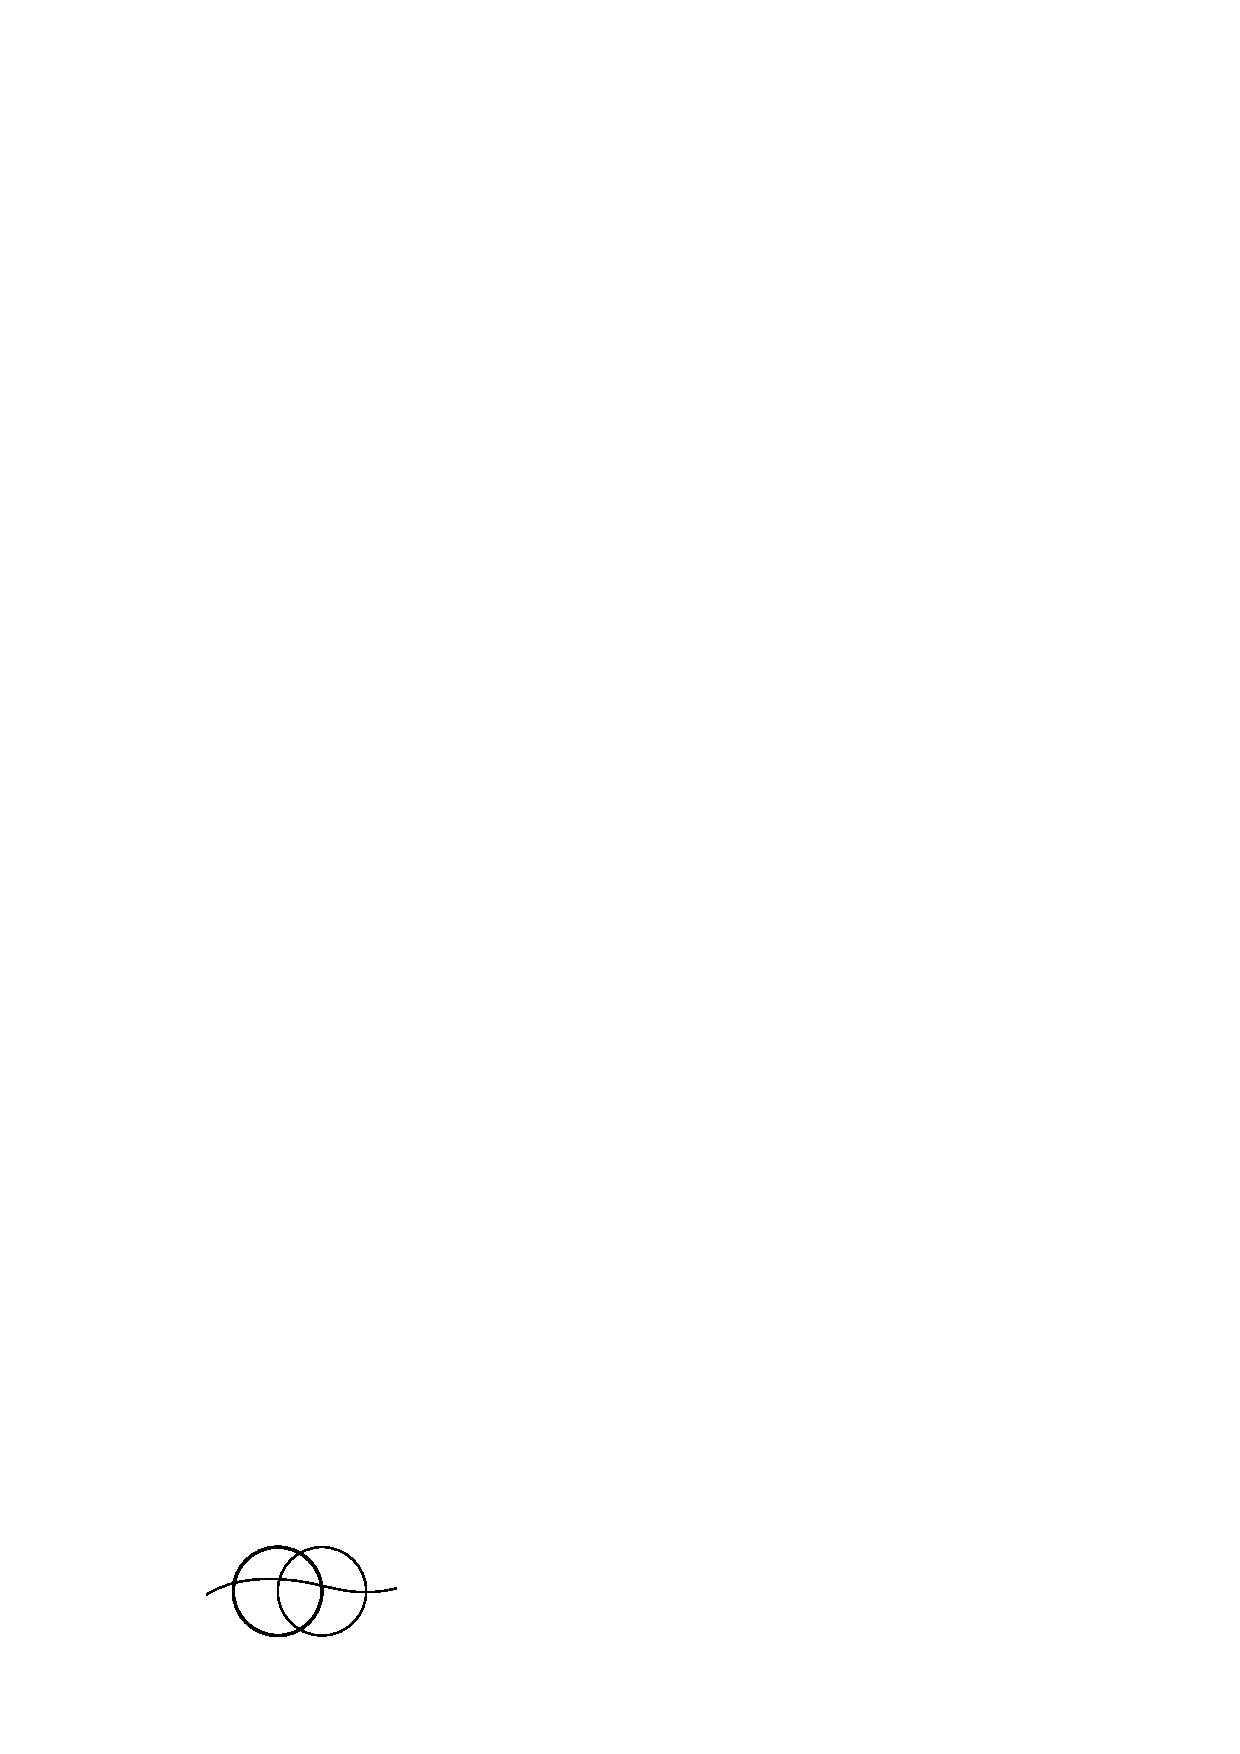
\includegraphics{graphics/mygraphic1.pdf}
  \else
    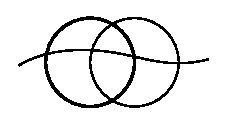
\includegraphics{graphics/mygraphic1-for-ps.eps}
  \fi
  \caption{Two circles and a wavy line.}
\end{figure}



\chapter{Conclusion and open questions}
\label{chap:conclusion}

This kind of chapter can include may different things (or only some of them):
\begin{itemize}
\item Discussion of results
\item Conclusions from the results or from the process in general
\item Open questions for future research, resulting from the research performed or from the results obtained
\end{itemize}

But not things like the bibliography or other back matter which is generated outside of this chapter.


\section{Some conclusion}

Here is what I conclude.

\section{Some open questions}

\paragraph{A question in brief.} In \autoref{chap:firstchap} we explored a certain subject, but what about this-or-that idea? Perhaps it is worth exploring. Can one produce interesting results?

\paragraph{A second question in brief.} A broader exposition of the question and indications of directions or ideas regarding its resolution.


%
% Add any appendices here; they must come _before_ the bibliography
%
\appendix
%\noappendicestocpagenum
%\addappheadtotoc

\chapter{Some sort of an appendix}
\label{appendix:somesort}

You may want to include appendices of your own volition. Also, if you've developed any computer software, that needs to go in as an appendix as well.

\section{A section}

Some appendix content here. And something nice to finish things off:

\begin{figure}[htb]
  \centering
  \ifpdf
    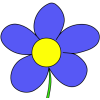
\includegraphics[width=0.3\textwidth]{graphics/mygraphic2.png}
  \else
    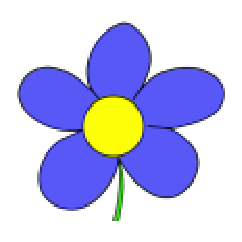
\includegraphics[width=0.3\textwidth]{graphics/mygraphic2-for-ps.eps}
  \fi
  \caption{A Flower.}
\end{figure}



% Back Matter
% ------------

% The following command will typeset the bibliography,
% then typeset the Hebrew part of the thesis:
% - Cover page
% - Title page
% - Acknowledgements page
%  (NO table of contents or list of figures in Hebrew)
% - (Extended) abstract (1000-2000 words)
%
% based on information you've provided in the thesis-fields file
% (including the relative paths to your bib files). The Hebrew
% content will be typeset in _reverse_page_order_, i.e. first
% in the file will be the last page of the abstract, and the
% Hebrew cover page will be the last page of the file.
%
\makebackmatter

% The resulting PDF can be printed and taken straight to binding,
% i.e. you do not need to flip any pages anywhere. Of course,
% mind the LaTeX error and warning messages, overfull hboxes etc.

\end{document}

